% Options for packages loaded elsewhere
\PassOptionsToPackage{unicode}{hyperref}
\PassOptionsToPackage{hyphens}{url}
%
\documentclass[
]{book}
\title{Tools for Estimating, Measuring and Working with Migration Data in R}
\author{Guy J. Abel, James Raymer, Ellen Kraly}
\date{2021-10-18}

\usepackage{amsmath,amssymb}
\usepackage{lmodern}
\usepackage{iftex}
\ifPDFTeX
  \usepackage[T1]{fontenc}
  \usepackage[utf8]{inputenc}
  \usepackage{textcomp} % provide euro and other symbols
\else % if luatex or xetex
  \usepackage{unicode-math}
  \defaultfontfeatures{Scale=MatchLowercase}
  \defaultfontfeatures[\rmfamily]{Ligatures=TeX,Scale=1}
\fi
% Use upquote if available, for straight quotes in verbatim environments
\IfFileExists{upquote.sty}{\usepackage{upquote}}{}
\IfFileExists{microtype.sty}{% use microtype if available
  \usepackage[]{microtype}
  \UseMicrotypeSet[protrusion]{basicmath} % disable protrusion for tt fonts
}{}
\makeatletter
\@ifundefined{KOMAClassName}{% if non-KOMA class
  \IfFileExists{parskip.sty}{%
    \usepackage{parskip}
  }{% else
    \setlength{\parindent}{0pt}
    \setlength{\parskip}{6pt plus 2pt minus 1pt}}
}{% if KOMA class
  \KOMAoptions{parskip=half}}
\makeatother
\usepackage{xcolor}
\IfFileExists{xurl.sty}{\usepackage{xurl}}{} % add URL line breaks if available
\IfFileExists{bookmark.sty}{\usepackage{bookmark}}{\usepackage{hyperref}}
\hypersetup{
  pdftitle={Tools for Estimating, Measuring and Working with Migration Data in R},
  pdfauthor={Guy J. Abel, James Raymer, Ellen Kraly},
  hidelinks,
  pdfcreator={LaTeX via pandoc}}
\urlstyle{same} % disable monospaced font for URLs
\usepackage{color}
\usepackage{fancyvrb}
\newcommand{\VerbBar}{|}
\newcommand{\VERB}{\Verb[commandchars=\\\{\}]}
\DefineVerbatimEnvironment{Highlighting}{Verbatim}{commandchars=\\\{\}}
% Add ',fontsize=\small' for more characters per line
\usepackage{framed}
\definecolor{shadecolor}{RGB}{248,248,248}
\newenvironment{Shaded}{\begin{snugshade}}{\end{snugshade}}
\newcommand{\AlertTok}[1]{\textcolor[rgb]{0.94,0.16,0.16}{#1}}
\newcommand{\AnnotationTok}[1]{\textcolor[rgb]{0.56,0.35,0.01}{\textbf{\textit{#1}}}}
\newcommand{\AttributeTok}[1]{\textcolor[rgb]{0.77,0.63,0.00}{#1}}
\newcommand{\BaseNTok}[1]{\textcolor[rgb]{0.00,0.00,0.81}{#1}}
\newcommand{\BuiltInTok}[1]{#1}
\newcommand{\CharTok}[1]{\textcolor[rgb]{0.31,0.60,0.02}{#1}}
\newcommand{\CommentTok}[1]{\textcolor[rgb]{0.56,0.35,0.01}{\textit{#1}}}
\newcommand{\CommentVarTok}[1]{\textcolor[rgb]{0.56,0.35,0.01}{\textbf{\textit{#1}}}}
\newcommand{\ConstantTok}[1]{\textcolor[rgb]{0.00,0.00,0.00}{#1}}
\newcommand{\ControlFlowTok}[1]{\textcolor[rgb]{0.13,0.29,0.53}{\textbf{#1}}}
\newcommand{\DataTypeTok}[1]{\textcolor[rgb]{0.13,0.29,0.53}{#1}}
\newcommand{\DecValTok}[1]{\textcolor[rgb]{0.00,0.00,0.81}{#1}}
\newcommand{\DocumentationTok}[1]{\textcolor[rgb]{0.56,0.35,0.01}{\textbf{\textit{#1}}}}
\newcommand{\ErrorTok}[1]{\textcolor[rgb]{0.64,0.00,0.00}{\textbf{#1}}}
\newcommand{\ExtensionTok}[1]{#1}
\newcommand{\FloatTok}[1]{\textcolor[rgb]{0.00,0.00,0.81}{#1}}
\newcommand{\FunctionTok}[1]{\textcolor[rgb]{0.00,0.00,0.00}{#1}}
\newcommand{\ImportTok}[1]{#1}
\newcommand{\InformationTok}[1]{\textcolor[rgb]{0.56,0.35,0.01}{\textbf{\textit{#1}}}}
\newcommand{\KeywordTok}[1]{\textcolor[rgb]{0.13,0.29,0.53}{\textbf{#1}}}
\newcommand{\NormalTok}[1]{#1}
\newcommand{\OperatorTok}[1]{\textcolor[rgb]{0.81,0.36,0.00}{\textbf{#1}}}
\newcommand{\OtherTok}[1]{\textcolor[rgb]{0.56,0.35,0.01}{#1}}
\newcommand{\PreprocessorTok}[1]{\textcolor[rgb]{0.56,0.35,0.01}{\textit{#1}}}
\newcommand{\RegionMarkerTok}[1]{#1}
\newcommand{\SpecialCharTok}[1]{\textcolor[rgb]{0.00,0.00,0.00}{#1}}
\newcommand{\SpecialStringTok}[1]{\textcolor[rgb]{0.31,0.60,0.02}{#1}}
\newcommand{\StringTok}[1]{\textcolor[rgb]{0.31,0.60,0.02}{#1}}
\newcommand{\VariableTok}[1]{\textcolor[rgb]{0.00,0.00,0.00}{#1}}
\newcommand{\VerbatimStringTok}[1]{\textcolor[rgb]{0.31,0.60,0.02}{#1}}
\newcommand{\WarningTok}[1]{\textcolor[rgb]{0.56,0.35,0.01}{\textbf{\textit{#1}}}}
\usepackage{longtable,booktabs,array}
\usepackage{calc} % for calculating minipage widths
% Correct order of tables after \paragraph or \subparagraph
\usepackage{etoolbox}
\makeatletter
\patchcmd\longtable{\par}{\if@noskipsec\mbox{}\fi\par}{}{}
\makeatother
% Allow footnotes in longtable head/foot
\IfFileExists{footnotehyper.sty}{\usepackage{footnotehyper}}{\usepackage{footnote}}
\makesavenoteenv{longtable}
\usepackage{graphicx}
\makeatletter
\def\maxwidth{\ifdim\Gin@nat@width>\linewidth\linewidth\else\Gin@nat@width\fi}
\def\maxheight{\ifdim\Gin@nat@height>\textheight\textheight\else\Gin@nat@height\fi}
\makeatother
% Scale images if necessary, so that they will not overflow the page
% margins by default, and it is still possible to overwrite the defaults
% using explicit options in \includegraphics[width, height, ...]{}
\setkeys{Gin}{width=\maxwidth,height=\maxheight,keepaspectratio}
% Set default figure placement to htbp
\makeatletter
\def\fps@figure{htbp}
\makeatother
\setlength{\emergencystretch}{3em} % prevent overfull lines
\providecommand{\tightlist}{%
  \setlength{\itemsep}{0pt}\setlength{\parskip}{0pt}}
\setcounter{secnumdepth}{5}
\usepackage{booktabs}
\usepackage{multirow}
\ifLuaTeX
  \usepackage{selnolig}  % disable illegal ligatures
\fi
\usepackage[]{natbib}
\bibliographystyle{plainnat}

\begin{document}
\maketitle

{
\setcounter{tocdepth}{1}
\tableofcontents
}
\hypertarget{section}{%
\chapter{.}\label{section}}

\hypertarget{outline}{%
\chapter{Outline}\label{outline}}

\hypertarget{workshop-on-migration-estimation}{%
\section{Workshop on Migration Estimation}\label{workshop-on-migration-estimation}}

\begin{itemize}
\tightlist
\item
  Course outline

  \begin{itemize}
  \tightlist
  \item
    Part 1: Migration data and concepts
  \item
    Part 2: Handling migration data in R
  \item
    Part 3: Summary migration indices
  \item
    Part 4: Estimating net migration
  \item
    Part 5: Describing and estimating migration age structure
  \item
    Part 6: Describing bilateral migration data
  \item
    Part 7: Estimating bilateral migration
  \item
    Part 8: Chord diagrams for visualising bilateral migration
  \item
    Part 9: Sankey plots for visualising bilateral migration
  \end{itemize}
\item
  Folder with slides, code in slides, exercises and exercise solutions on dropbox

  \begin{itemize}
  \tightlist
  \item
    \texttt{http://bit.ly/kostat2021mig}
  \end{itemize}
\item
  The \texttt{slides-code} folder contains the R functions in the PDF's of each slide

  \begin{itemize}
  \tightlist
  \item
    Ignore the first few lines (with \texttt{knitr} functions) - they are by-product of using Rmarkdown to create the slide PDFs
  \end{itemize}
\end{itemize}

\hypertarget{general-points}{%
\section{General Points}\label{general-points}}

\begin{enumerate}
\def\labelenumi{\arabic{enumi}.}
\tightlist
\item
  Please be patient. Teaching classes that involve R is never smooth.

  \begin{itemize}
  \tightlist
  \item
    Everyone has different computers, R versions, package versions
  \item
    Remote learning and getting used to Zoom
  \end{itemize}
\item
  I am assuming you have some knowledge on using R, especially the \emph{tidyverse} set of packages. If you do not, then try working your way through an online course to get up to speed:

  \begin{itemize}
  \tightlist
  \item
    \texttt{https://r-bootcamp.netlify.app/} (free)
  \end{itemize}
\item
  Throughout the course we will work on some exercises. You might get stuck, especially if you are new to R. Be patient and remember that the frustration is a normal part of learning a programming language.
\item
  The exercise solutions are provided. If you do not have time to complete the exercises in class, spend some extra time to keep working on the exercises.

  \begin{itemize}
  \tightlist
  \item
    Some days we will not have time to finish all the exercises
  \end{itemize}
\item
  If you having trouble installing R, RStudio or the packages I have set up an RStudio cloud project where everything is installed for you:

  \begin{itemize}
  \tightlist
  \item
    \texttt{https://rstudio.cloud/project/1593361}
  \item
    Need to create a RStudio account
  \item
    Save changes using button on top right
  \end{itemize}
\end{enumerate}

\hypertarget{migration-concepts}{%
\chapter{Migration Concepts}\label{migration-concepts}}

\begin{itemize}
\tightlist
\item
  Migration involves a change in place of abode, or place of ``usual'' residence-a taking-up of life in a new or different place - \citet{UnitedNations1983}
\item
  Could apply to a range of demographic units, such as a person, a family or a household
\item
  Tend to excludes nomads, movement of population groups with no fixed place of residence, seasonal movements of persons who live in two or more places during the course of a year.
\item
  Both a spatial (place) and temporal (change) dimension are required in the definition of migration
\end{itemize}

\hypertarget{spatial}{%
\section{Spatial}\label{spatial}}

\hypertarget{place-of-residence}{%
\subsection{Place of Residence}\label{place-of-residence}}

The \emph{Principles and Recommendations for Population and Housing Censuses} (UN Statistics Division 2008: 102, para. 1.463) defines usual residence as follows:

``It is recommended that countries apply a threshold of 12 months when considering place of usual residence according to one of the following two criteria:

\begin{enumerate}
\def\labelenumi{\arabic{enumi}.}
\item
  The place at which the person has lived continuously for most of the last 12 months (that is, for at least six months and one day), not including temporary absences for holidays or work assignments, or intends to live for at least six months
\item
  The place at which the person has lived continuously for at least the last 12 months, not including temporary absences for holidays or work assignments, or intends to live for at least 12 months.''
\end{enumerate}

\hypertarget{place-of-residence-1}{%
\subsection{Place of Residence}\label{place-of-residence-1}}

\begin{itemize}
\tightlist
\item
  Typically no restriction is placed on the distance involved in a relocation - see \citet{Lee1966}.

  \begin{itemize}
  \tightlist
  \item
    Could include move from one apartment to another in the same building, or it may be a move to another country.
  \end{itemize}
\item
  In the past, some researchers have drawn a distinction between moves between local communities (cities, labour markets) and moves within local communities

  \begin{itemize}
  \tightlist
  \item
    Labelled as `migration' and `local mobility'.
  \item
    Many have argued that this distinction is problematic and no spatial constraints on the definition of migration should be used.
  \end{itemize}
\end{itemize}

\hypertarget{place-of-residence-2}{%
\subsection{Place of Residence}\label{place-of-residence-2}}

\begin{itemize}
\tightlist
\item
  If address information on points of origin and points of destination, the tabulation of moves by distance covered could be obtained.

  \begin{itemize}
  \tightlist
  \item
    Usually, not possible in countries without population registers
  \item
    Time consuming and of little policy relevance
  \end{itemize}
\item
  Census or survey results are necessarily tabulated for the administrative or political units into which the country is divided.
\item
  A migration is then operationally defined as a change of residence from one civil division to another, and the volume of migration is to a considerable degree a function of the size of areas chosen for compilation.
\end{itemize}

\hypertarget{courgeau-1979}{%
\subsection{Courgeau (1979)}\label{courgeau-1979}}

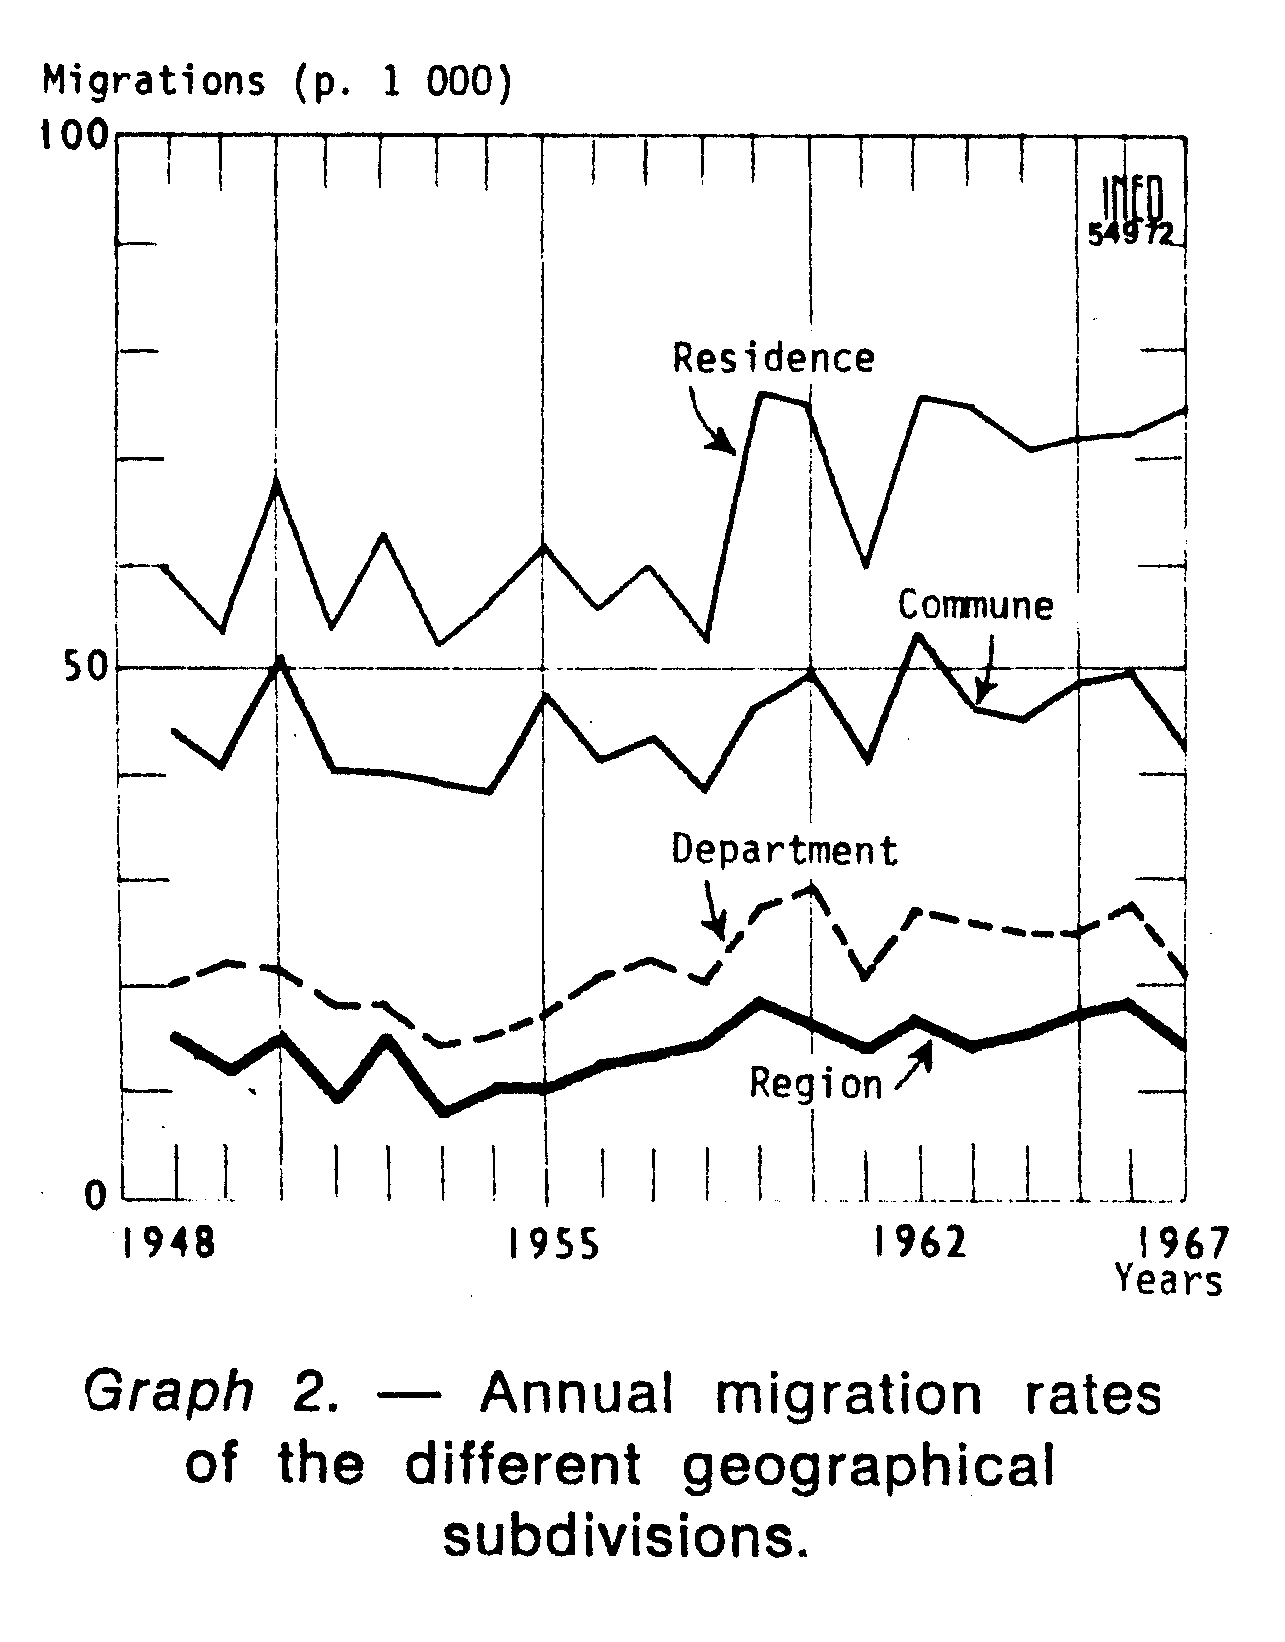
\includegraphics[width=0.5\linewidth]{img/courgeau-1979-area}

\hypertarget{place-of-origin}{%
\subsection{Place of Origin}\label{place-of-origin}}

\begin{itemize}
\tightlist
\item
  Typologies of migration data can be stratified by differing places of origin. Most commonly used:
\end{itemize}

\begin{longtable}[]{@{}ll@{}}
\toprule
Origin & Data Type \\
\midrule
\endhead
Previous place of residence & Migration event (movement) data \\
Place of residence \(n\) years ago & Migrant transition data \\
\bottomrule
\end{longtable}

\begin{itemize}
\tightlist
\item
  Lifetime migration data could be considered as a form of transition data where \(n\) changes based on the age of each individual

  \begin{itemize}
  \tightlist
  \item
    Migrant stock data are an aggregation over all persons lifetime migration flow.
  \item
    Given at specific point of time without an interval.
  \item
    Migration data literature often distinguishes between stock and flow data.
  \end{itemize}
\item
  Other types of migration data occasionally collected are

  \begin{itemize}
  \tightlist
  \item
    Duration at residence (combined with place of previous residence can derive a migration transitions)
  \item
    Number of moves over a given interval (event data)
  \item
    Country of citizenship (sometimes used as a proxy for place of birth)
  \end{itemize}
\end{itemize}

\hypertarget{migrant-transition-data}{%
\subsection{Migrant Transition Data}\label{migrant-transition-data}}

\begin{itemize}
\tightlist
\item
  Migrant transition data are typical collected in national censuses which identify migrants by comparing their place of usual residence at the time of enumeration (\(t\)) with that at a specified earlier date (\(t-n\)).

  \begin{itemize}
  \tightlist
  \item
    Time period is usually either 1 year (e.g.~UK) or 5 years (e.g.~USA)
  \item
    Some countries have time periods as the interval between current and last census or significant time point in countries history.
  \end{itemize}
\item
  Transition data fail to identify multiple and return moves, and migrants who are born or who die during the measurement period.
\end{itemize}

\hypertarget{migrant-transition-data---rees-1970}{%
\subsection{Migrant Transition Data - Rees 1970}\label{migrant-transition-data---rees-1970}}

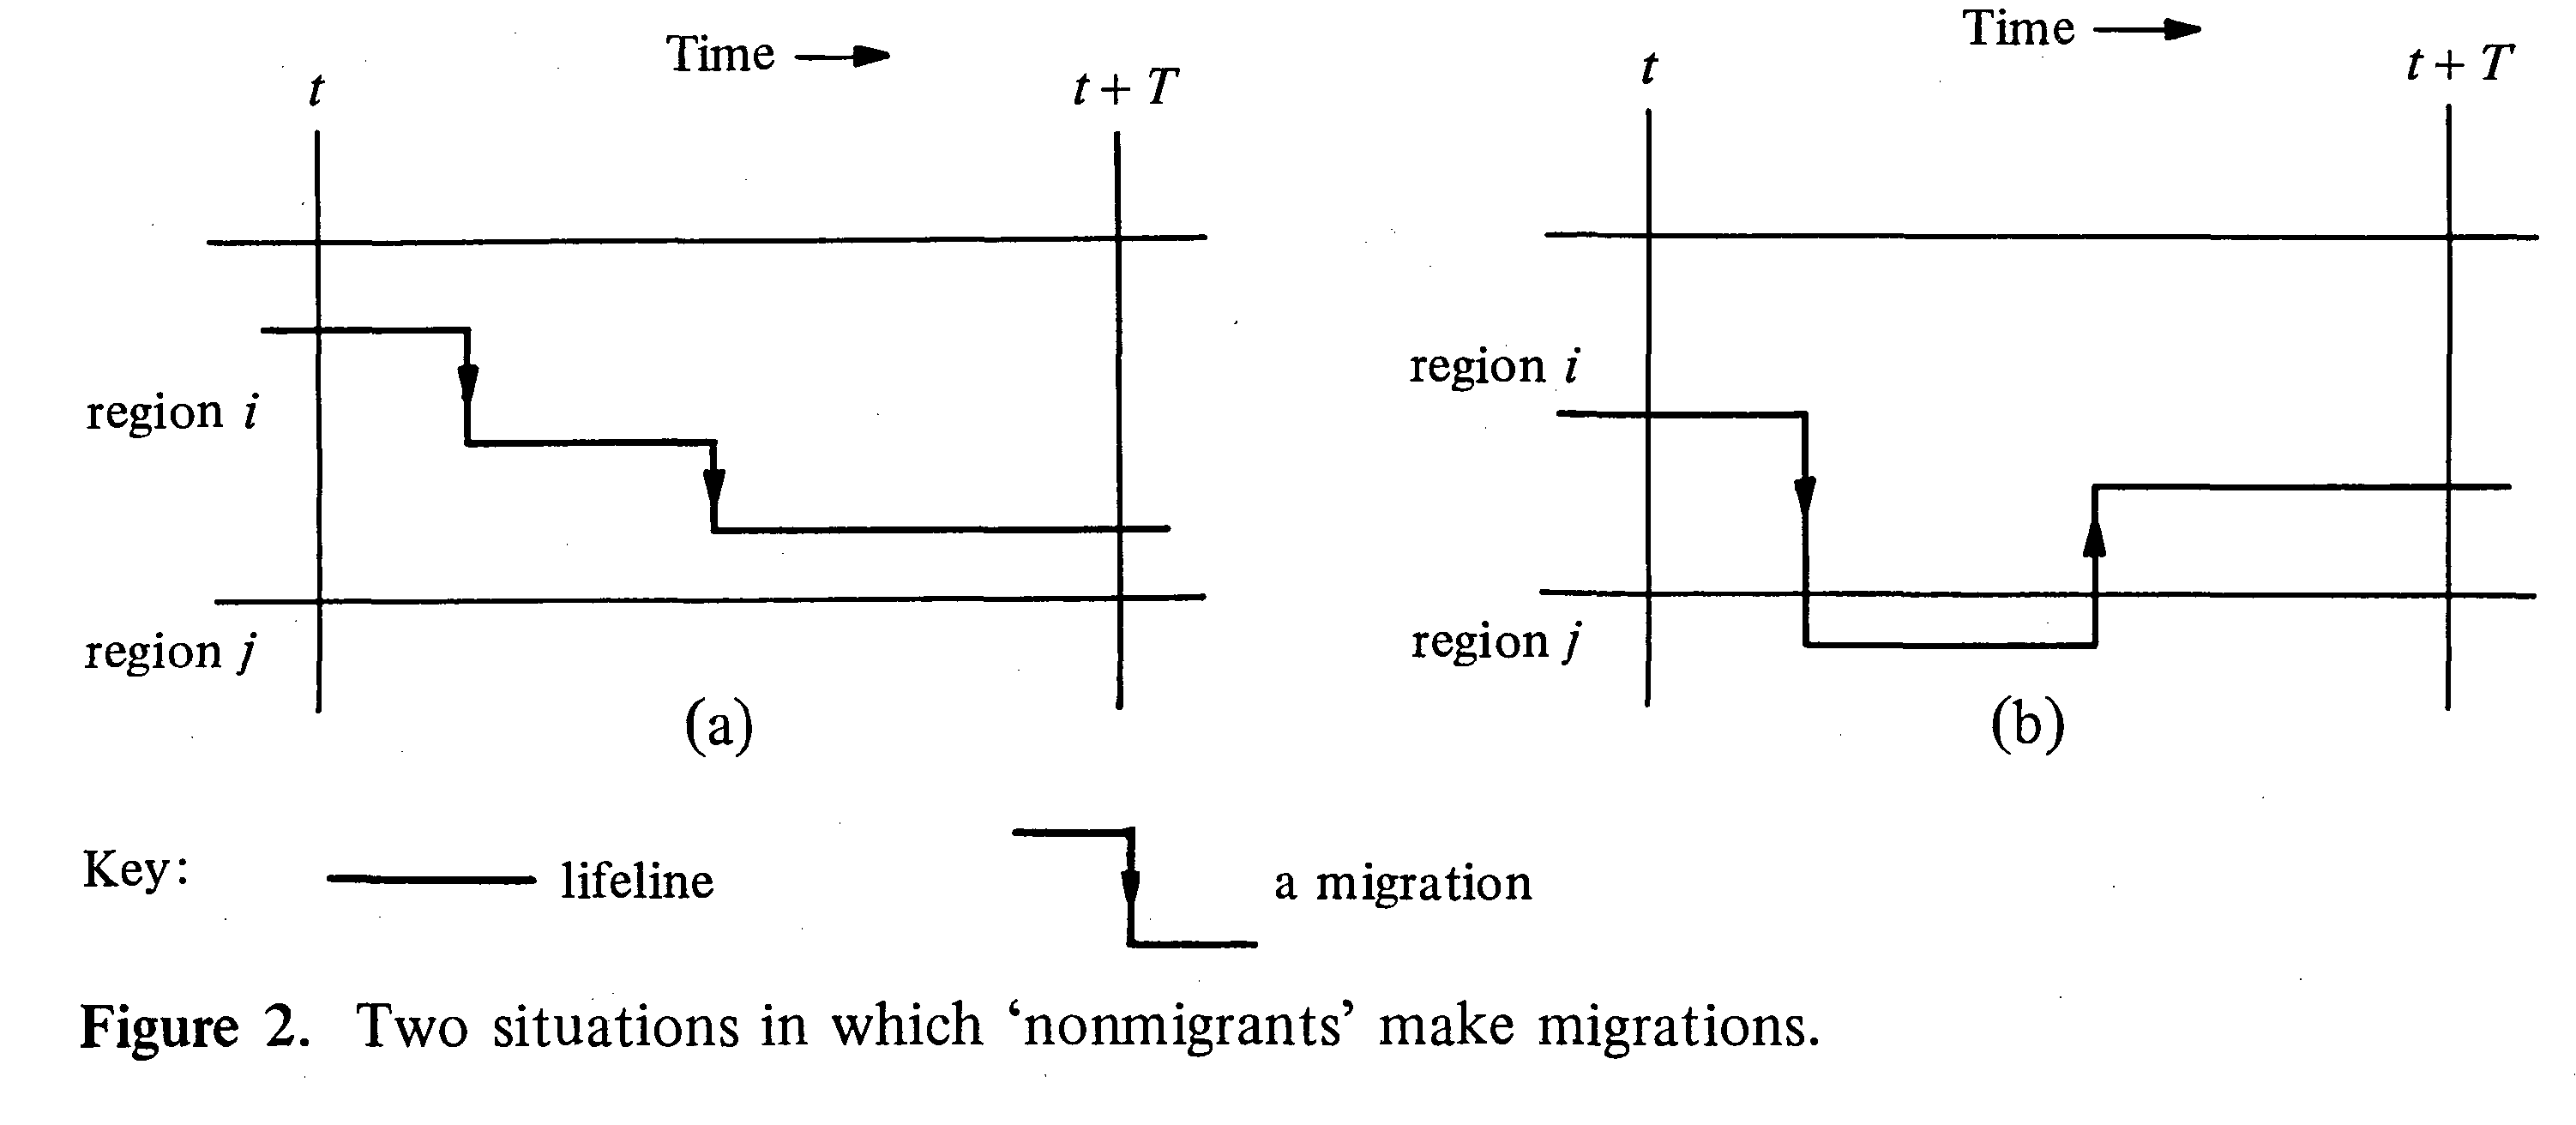
\includegraphics[width=1\linewidth]{img/rees-1977-non-migration}

\hypertarget{migrants-and-migration}{%
\subsection{Migrants and Migration}\label{migrants-and-migration}}

\begin{itemize}
\tightlist
\item
  Transition data are counts of migrants
\item
  A migrant is a person who has in some specified period in the past experienced one or more migrations.
\item
  Persons who moved during the interval and died before its end should, strictly speaking, be counted as migrants and their moves should be counted as migrations.

  \begin{itemize}
  \tightlist
  \item
    Likely to be excluded as information on migrants is usually obtained after the end of the interval and with reference to persons still living at that time.
  \end{itemize}
\end{itemize}

\hypertarget{migration-event-data}{%
\subsection{Migration Event Data}\label{migration-event-data}}

\begin{itemize}
\tightlist
\item
  Event data record every move that is made by each individual

  \begin{itemize}
  \tightlist
  \item
    Include multiple and return migrations as well as moves by the newborn and those immediately before death.
  \item
    Typically collected in population registers
  \item
    Represent a more complete record of migration over time
  \end{itemize}
\item
  Geographical units for which the data are available are generally coarser and registers often fail to capture information on within-region moves.
\item
  Less information about characteristics of migrants is usually available

  \begin{itemize}
  \tightlist
  \item
    Some groups may be omitted from altogether (e.g.~prisoners, military personnel)
  \end{itemize}
\end{itemize}

\hypertarget{migration-event-data-1}{%
\subsection{Migration Event Data}\label{migration-event-data-1}}

\begin{itemize}
\tightlist
\item
  There are important distinctions between the play (migration) and the actor (migrant).
\item
  For a given migration interval, the number of migrants is rarely, if ever, as large as the number of migrations.

  \begin{itemize}
  \tightlist
  \item
    Unless the interval is very short (a day, or perhaps a week) some persons are certain to move more than once.
  \item
    The longer the migration interval the more the count of migrants will understate the amount of migration.
  \item
    Conversely, the shorter the migration interval, the count of migrants will approach the number of migrations.
  \end{itemize}
\item
  Shown by \citet{Courgeau1979} \ldots{}
\end{itemize}

\hypertarget{migration-event-data---courgeau-1979}{%
\subsection{Migration Event Data - Courgeau (1979)}\label{migration-event-data---courgeau-1979}}

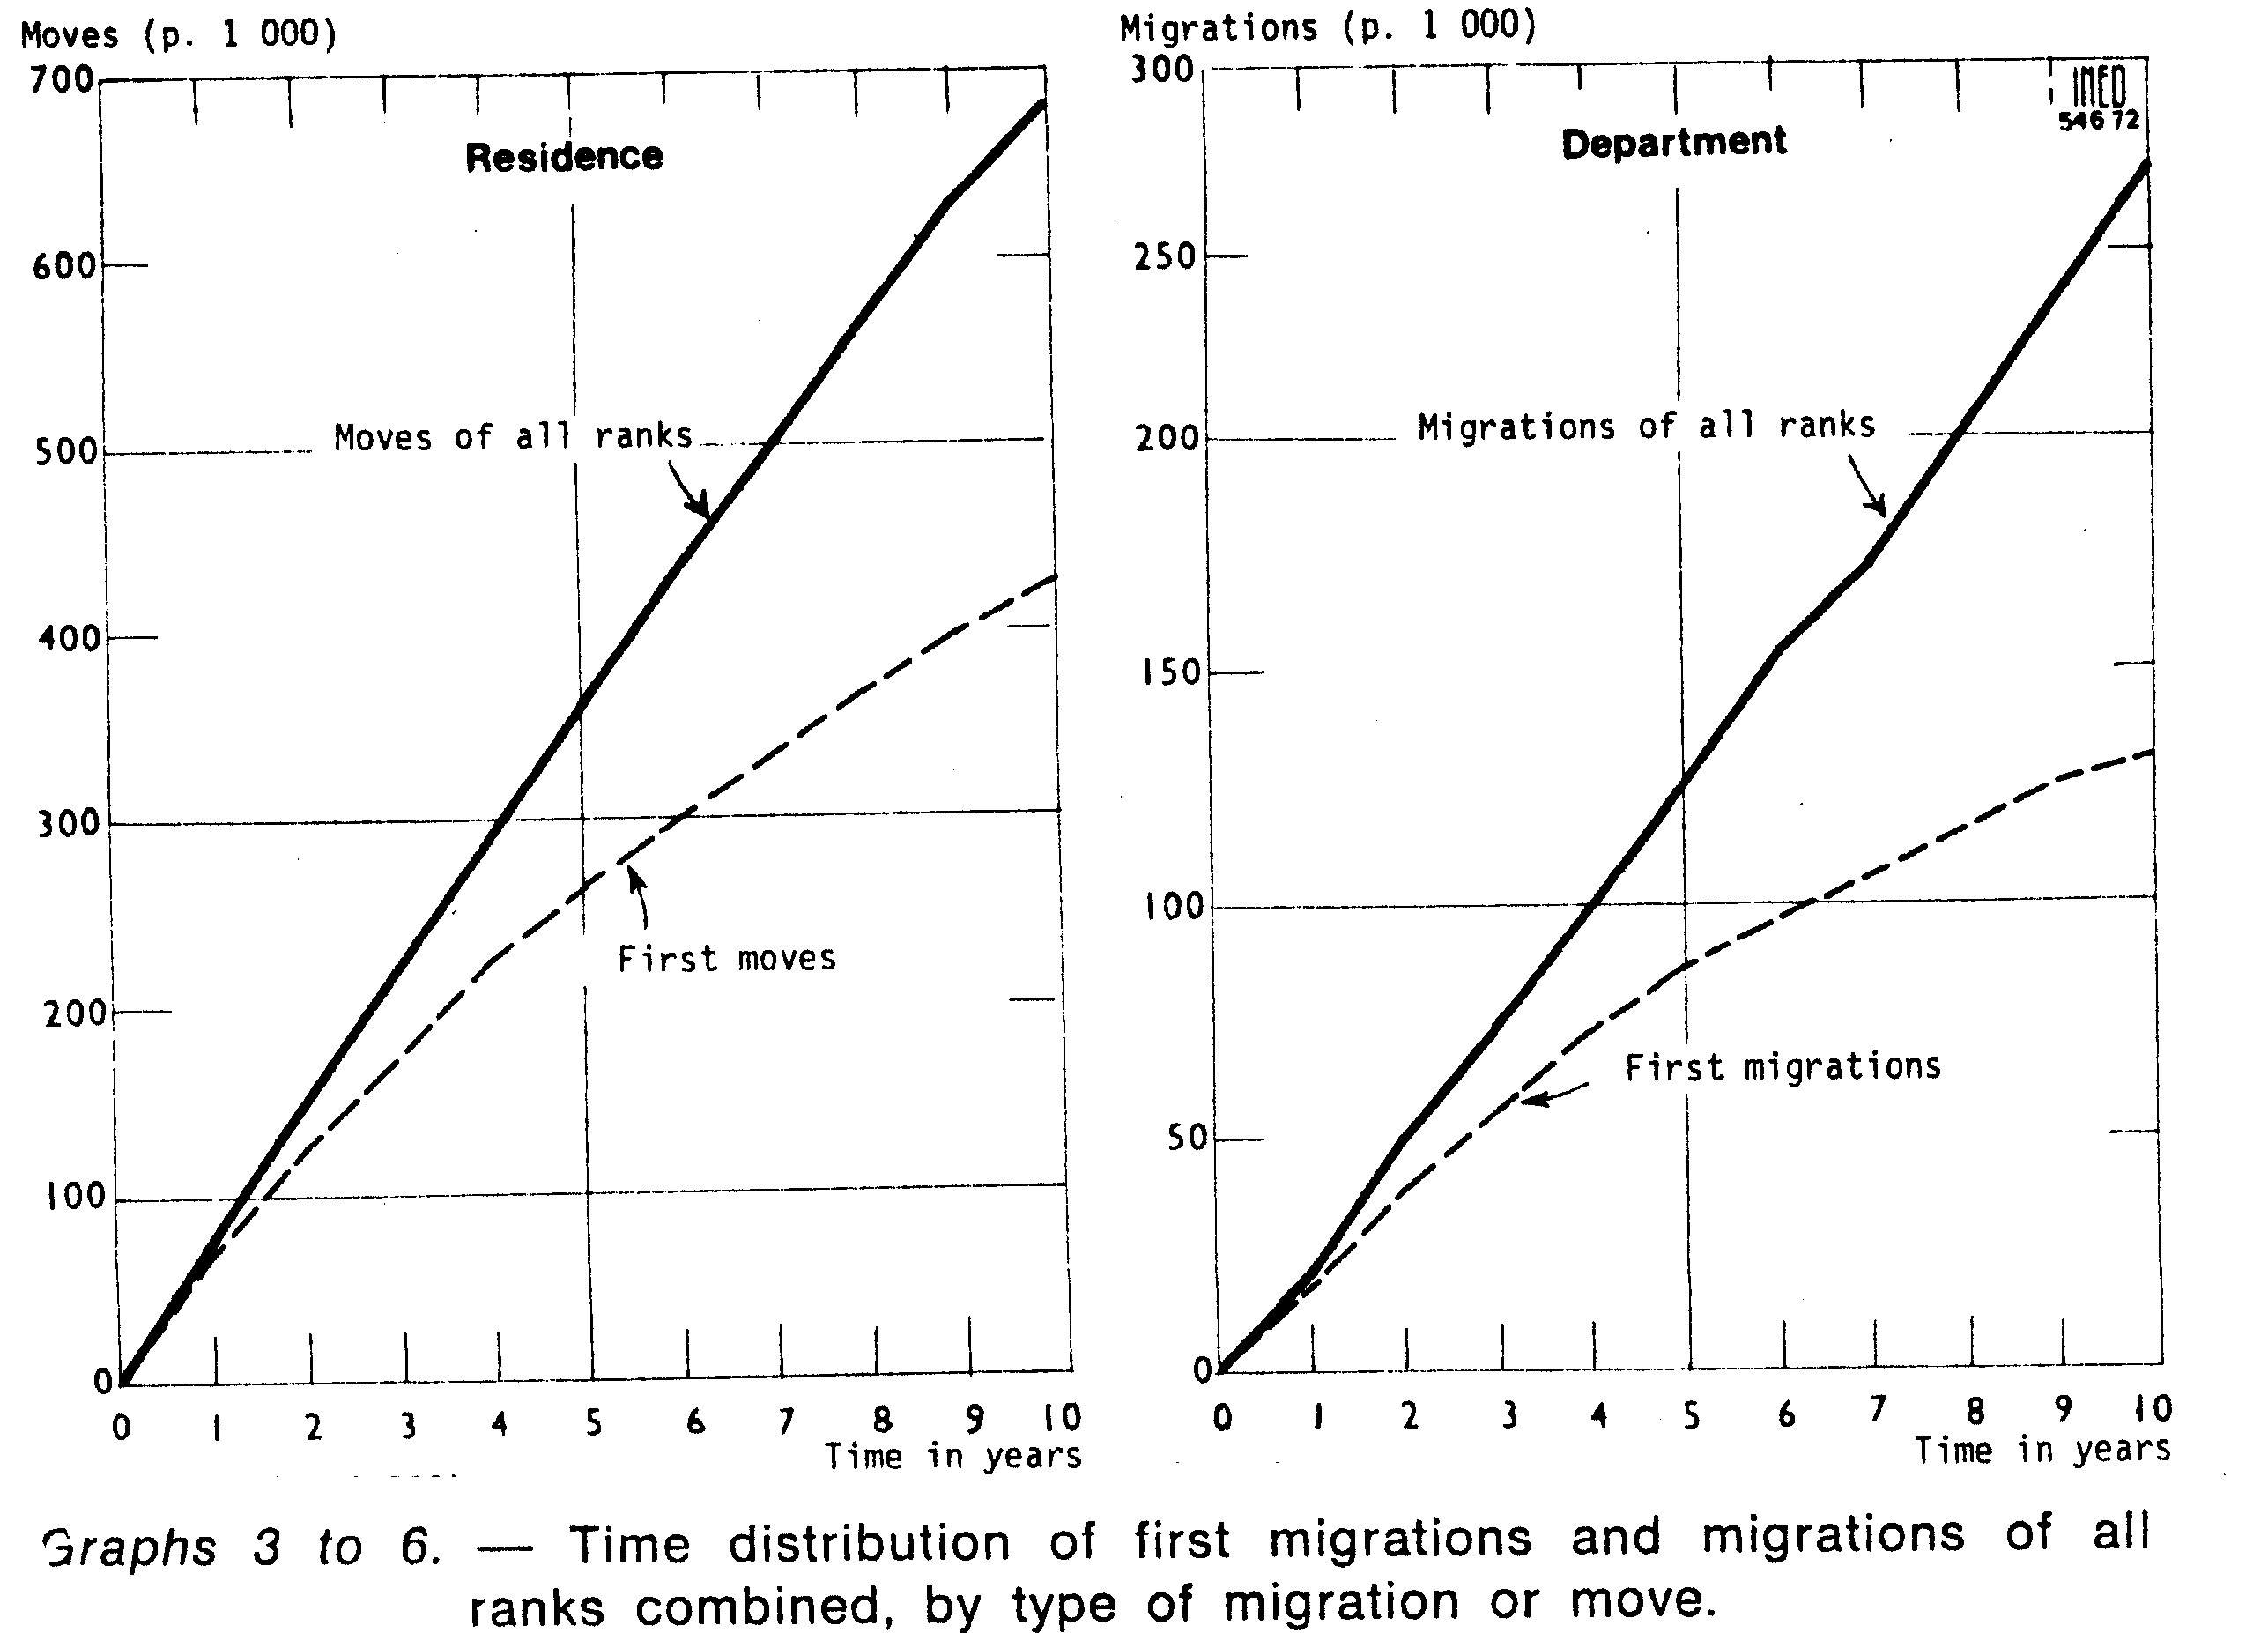
\includegraphics[width=0.9\linewidth]{img/courgeau-1979-period-a}

\hypertarget{migration-event-data-2}{%
\subsection{Migration Event Data}\label{migration-event-data-2}}

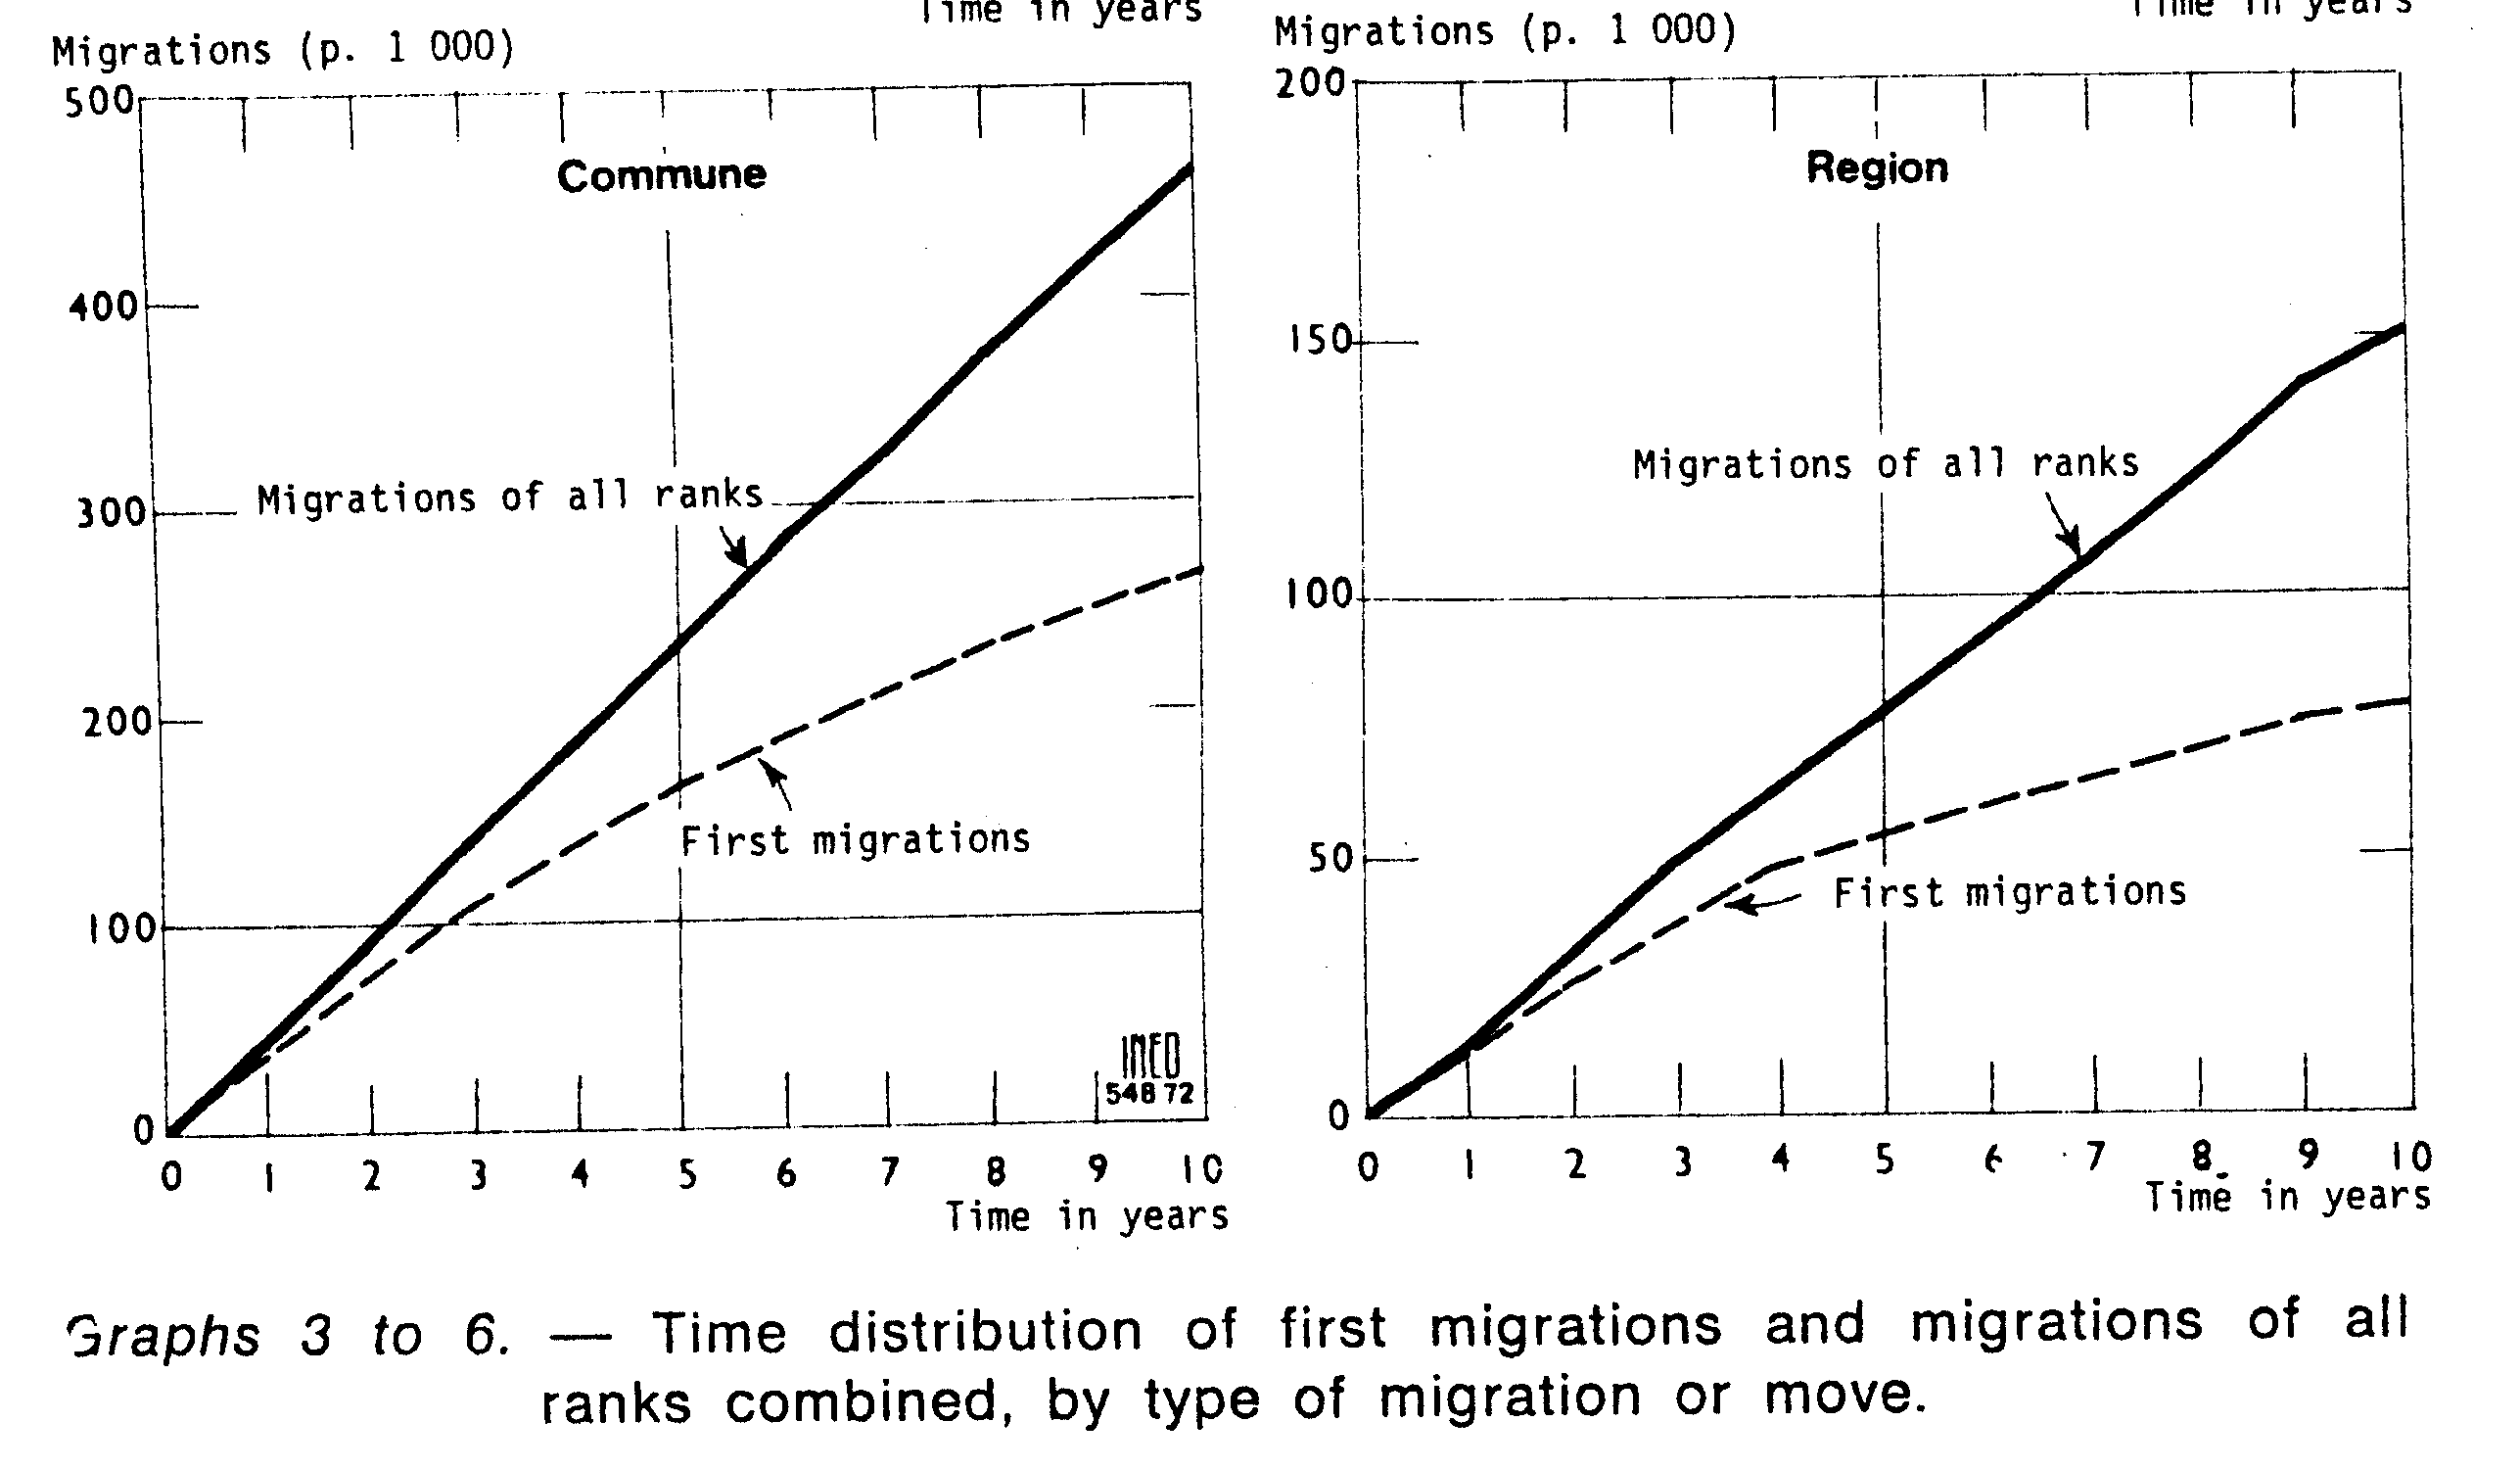
\includegraphics[width=0.9\linewidth]{img/courgeau-1979-period-b}

\hypertarget{temporal}{%
\section{Temporal}\label{temporal}}

\hypertarget{migration-interval}{%
\subsection{Migration Interval}\label{migration-interval}}

\begin{itemize}
\tightlist
\item
  Migration occurs continuously over time. In order to study its incidence, data have to be compiled
  with reference to specified periods of time.
\item
  The interval can be

  \begin{itemize}
  \tightlist
  \item
    Definite, e.g., one year, five years, ten years, the intercensal period
  \item
    Indefinite, e.g., the lifetime of the population alive at a given date.
  \end{itemize}
\item
  Definite interval data typically called fixed-term or period migration (or surviving migrants in the example on the next slide)
\item
  Lifetime migration or data based on place of last residence lack a definite time reference.
\end{itemize}

\hypertarget{migration-interval---rees-1977}{%
\subsection{Migration Interval - Rees (1977)}\label{migration-interval---rees-1977}}

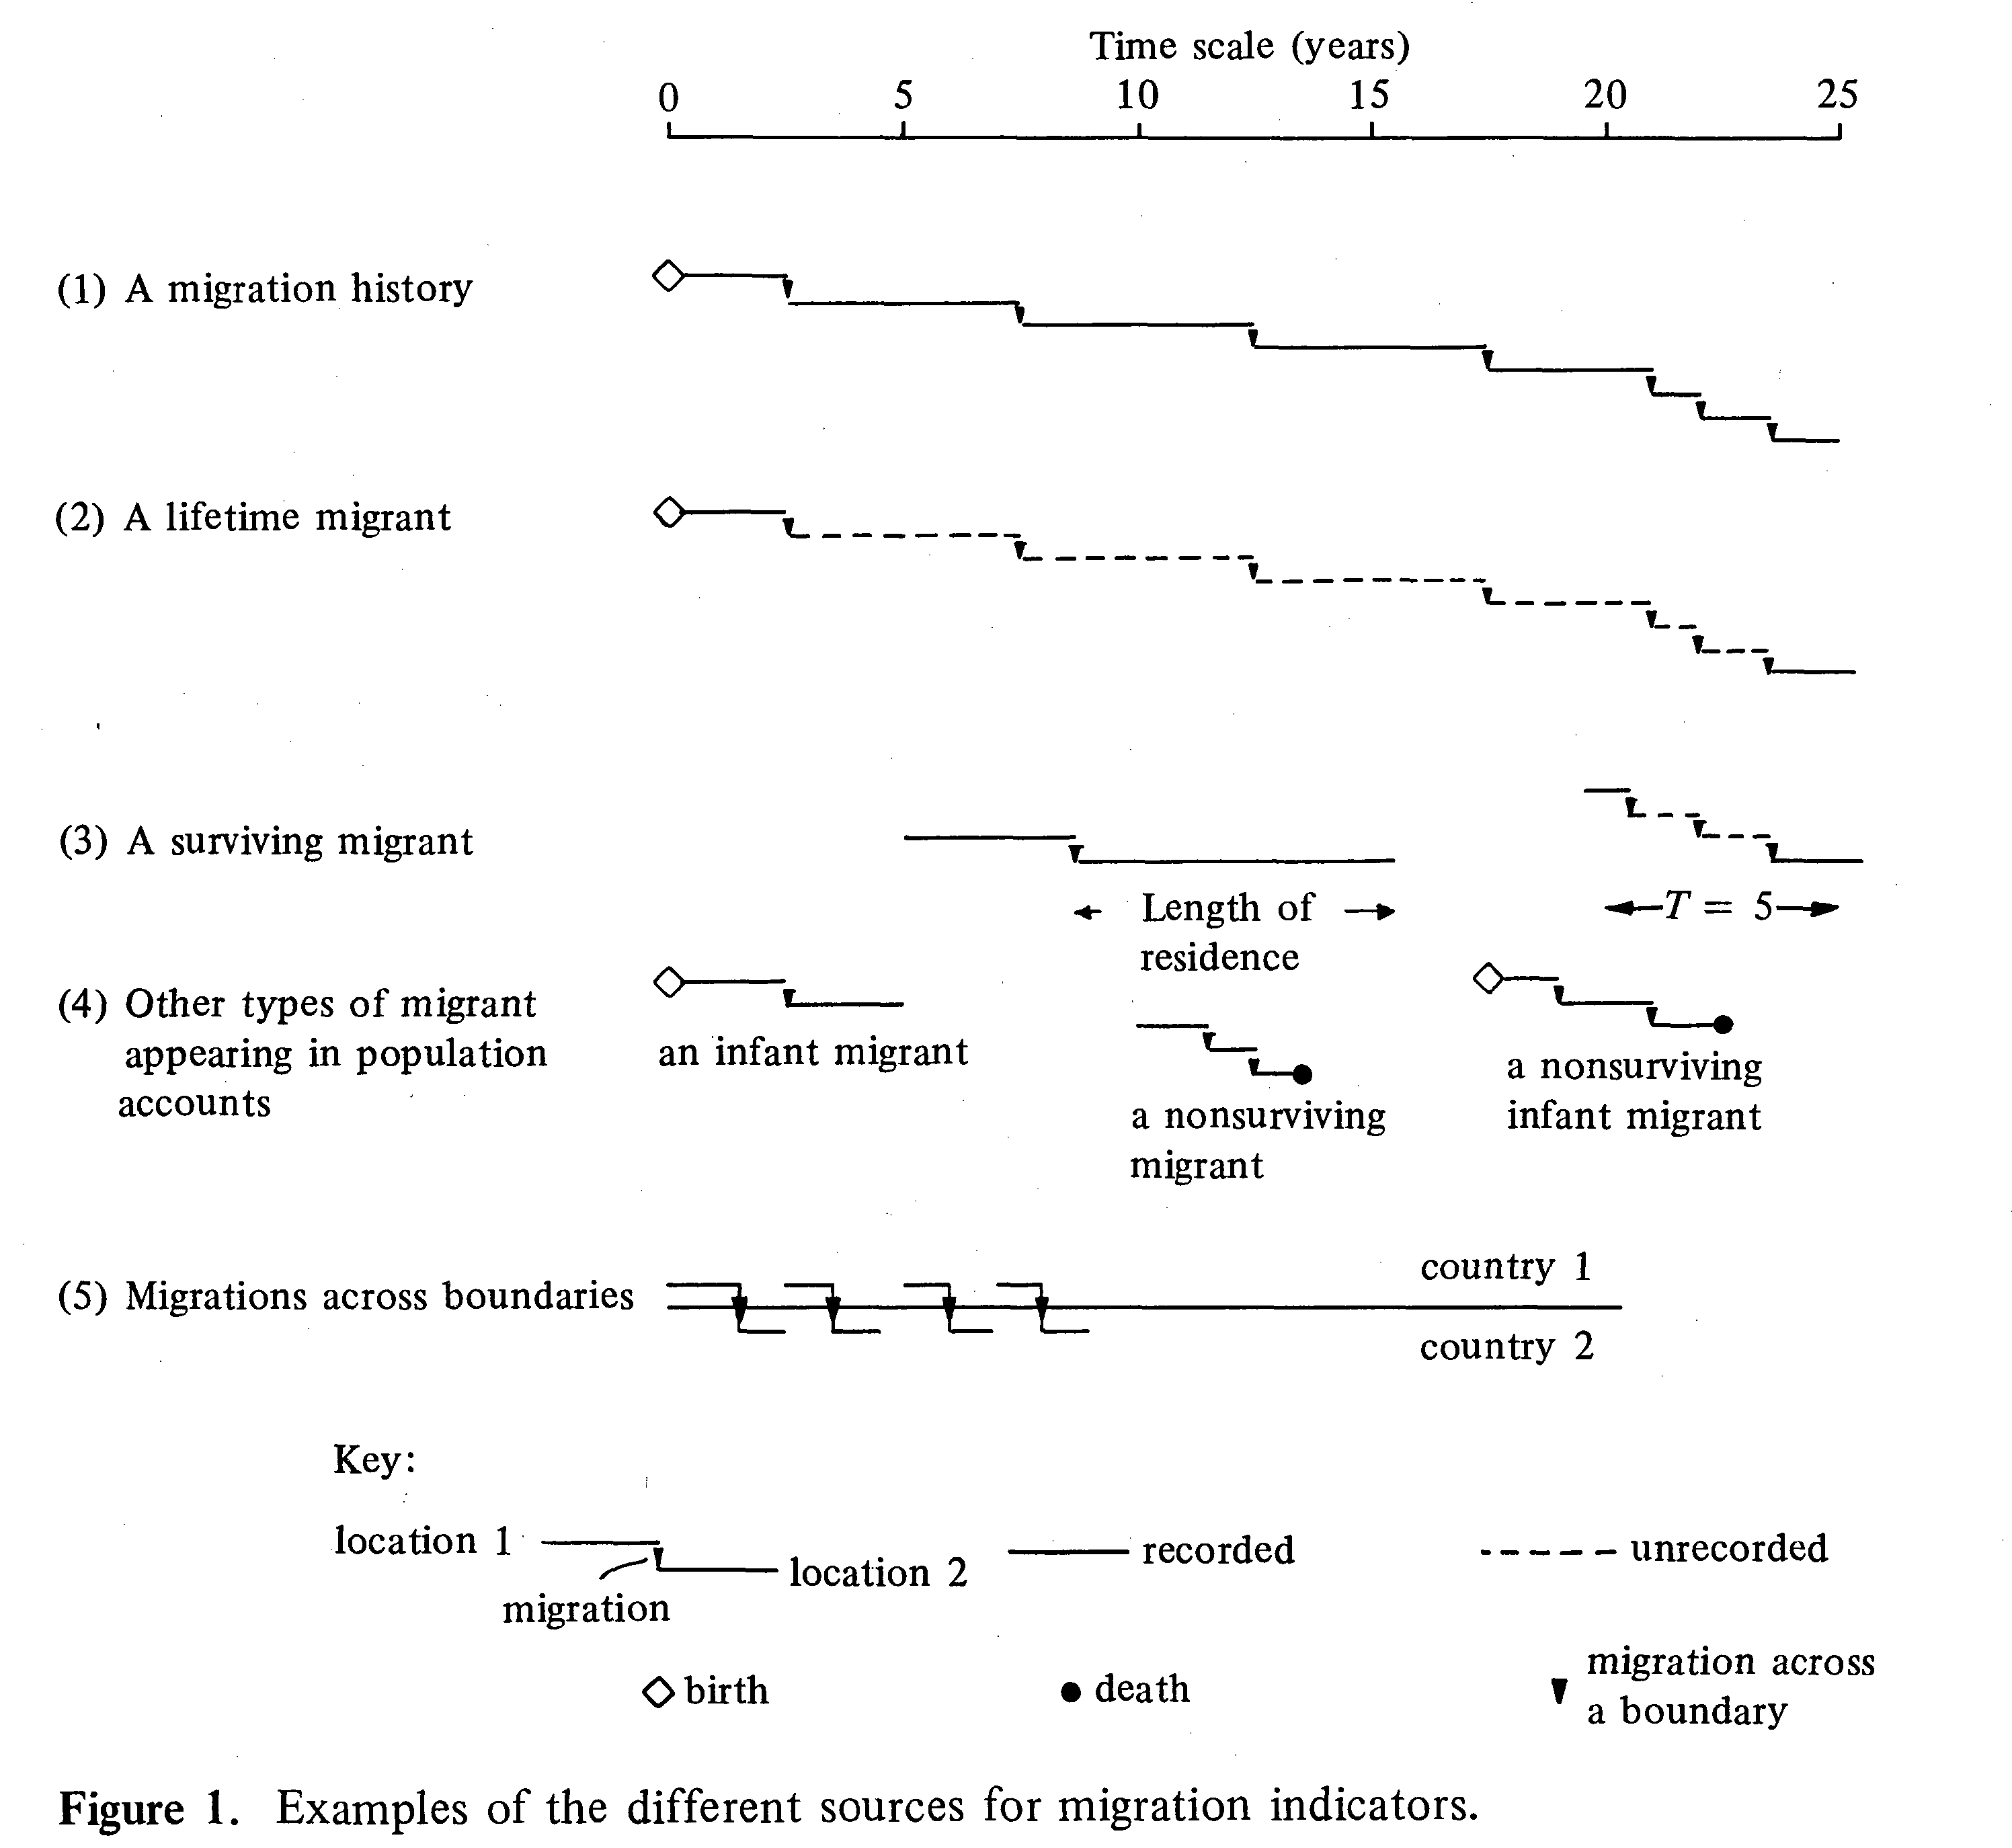
\includegraphics[width=0.75\linewidth]{img/rees-1977-types}

\hypertarget{one-year-five-year-problem}{%
\subsection{One-Year Five-Year Problem}\label{one-year-five-year-problem}}

\begin{itemize}
\tightlist
\item
  Migration data is commonly collected over a one or five year interval.
\item
  In places where both intervals are used, the number of migrants recorded over a five-year interval is far less than five times the number recorded over a one-year interval

  \begin{itemize}
  \tightlist
  \item
    Seen in Courgeau (1979) plots or Rees(1970) tables - see next slides
  \end{itemize}
\item
  \citet{Rogerson1990} no straightforward algebraic solution to comparing one-year and five-year migration probabilities.
\item
  Event data has similar patterns to transition data for the same period, however

  \begin{itemize}
  \tightlist
  \item
    Width of the interval influences the intensity of migration and also the geographic pattern of captured migration flows.
  \end{itemize}
\end{itemize}

\hypertarget{one-year-five-year-problem---rees-1970}{%
\subsection{One-Year Five-Year Problem - Rees 1970}\label{one-year-five-year-problem---rees-1970}}

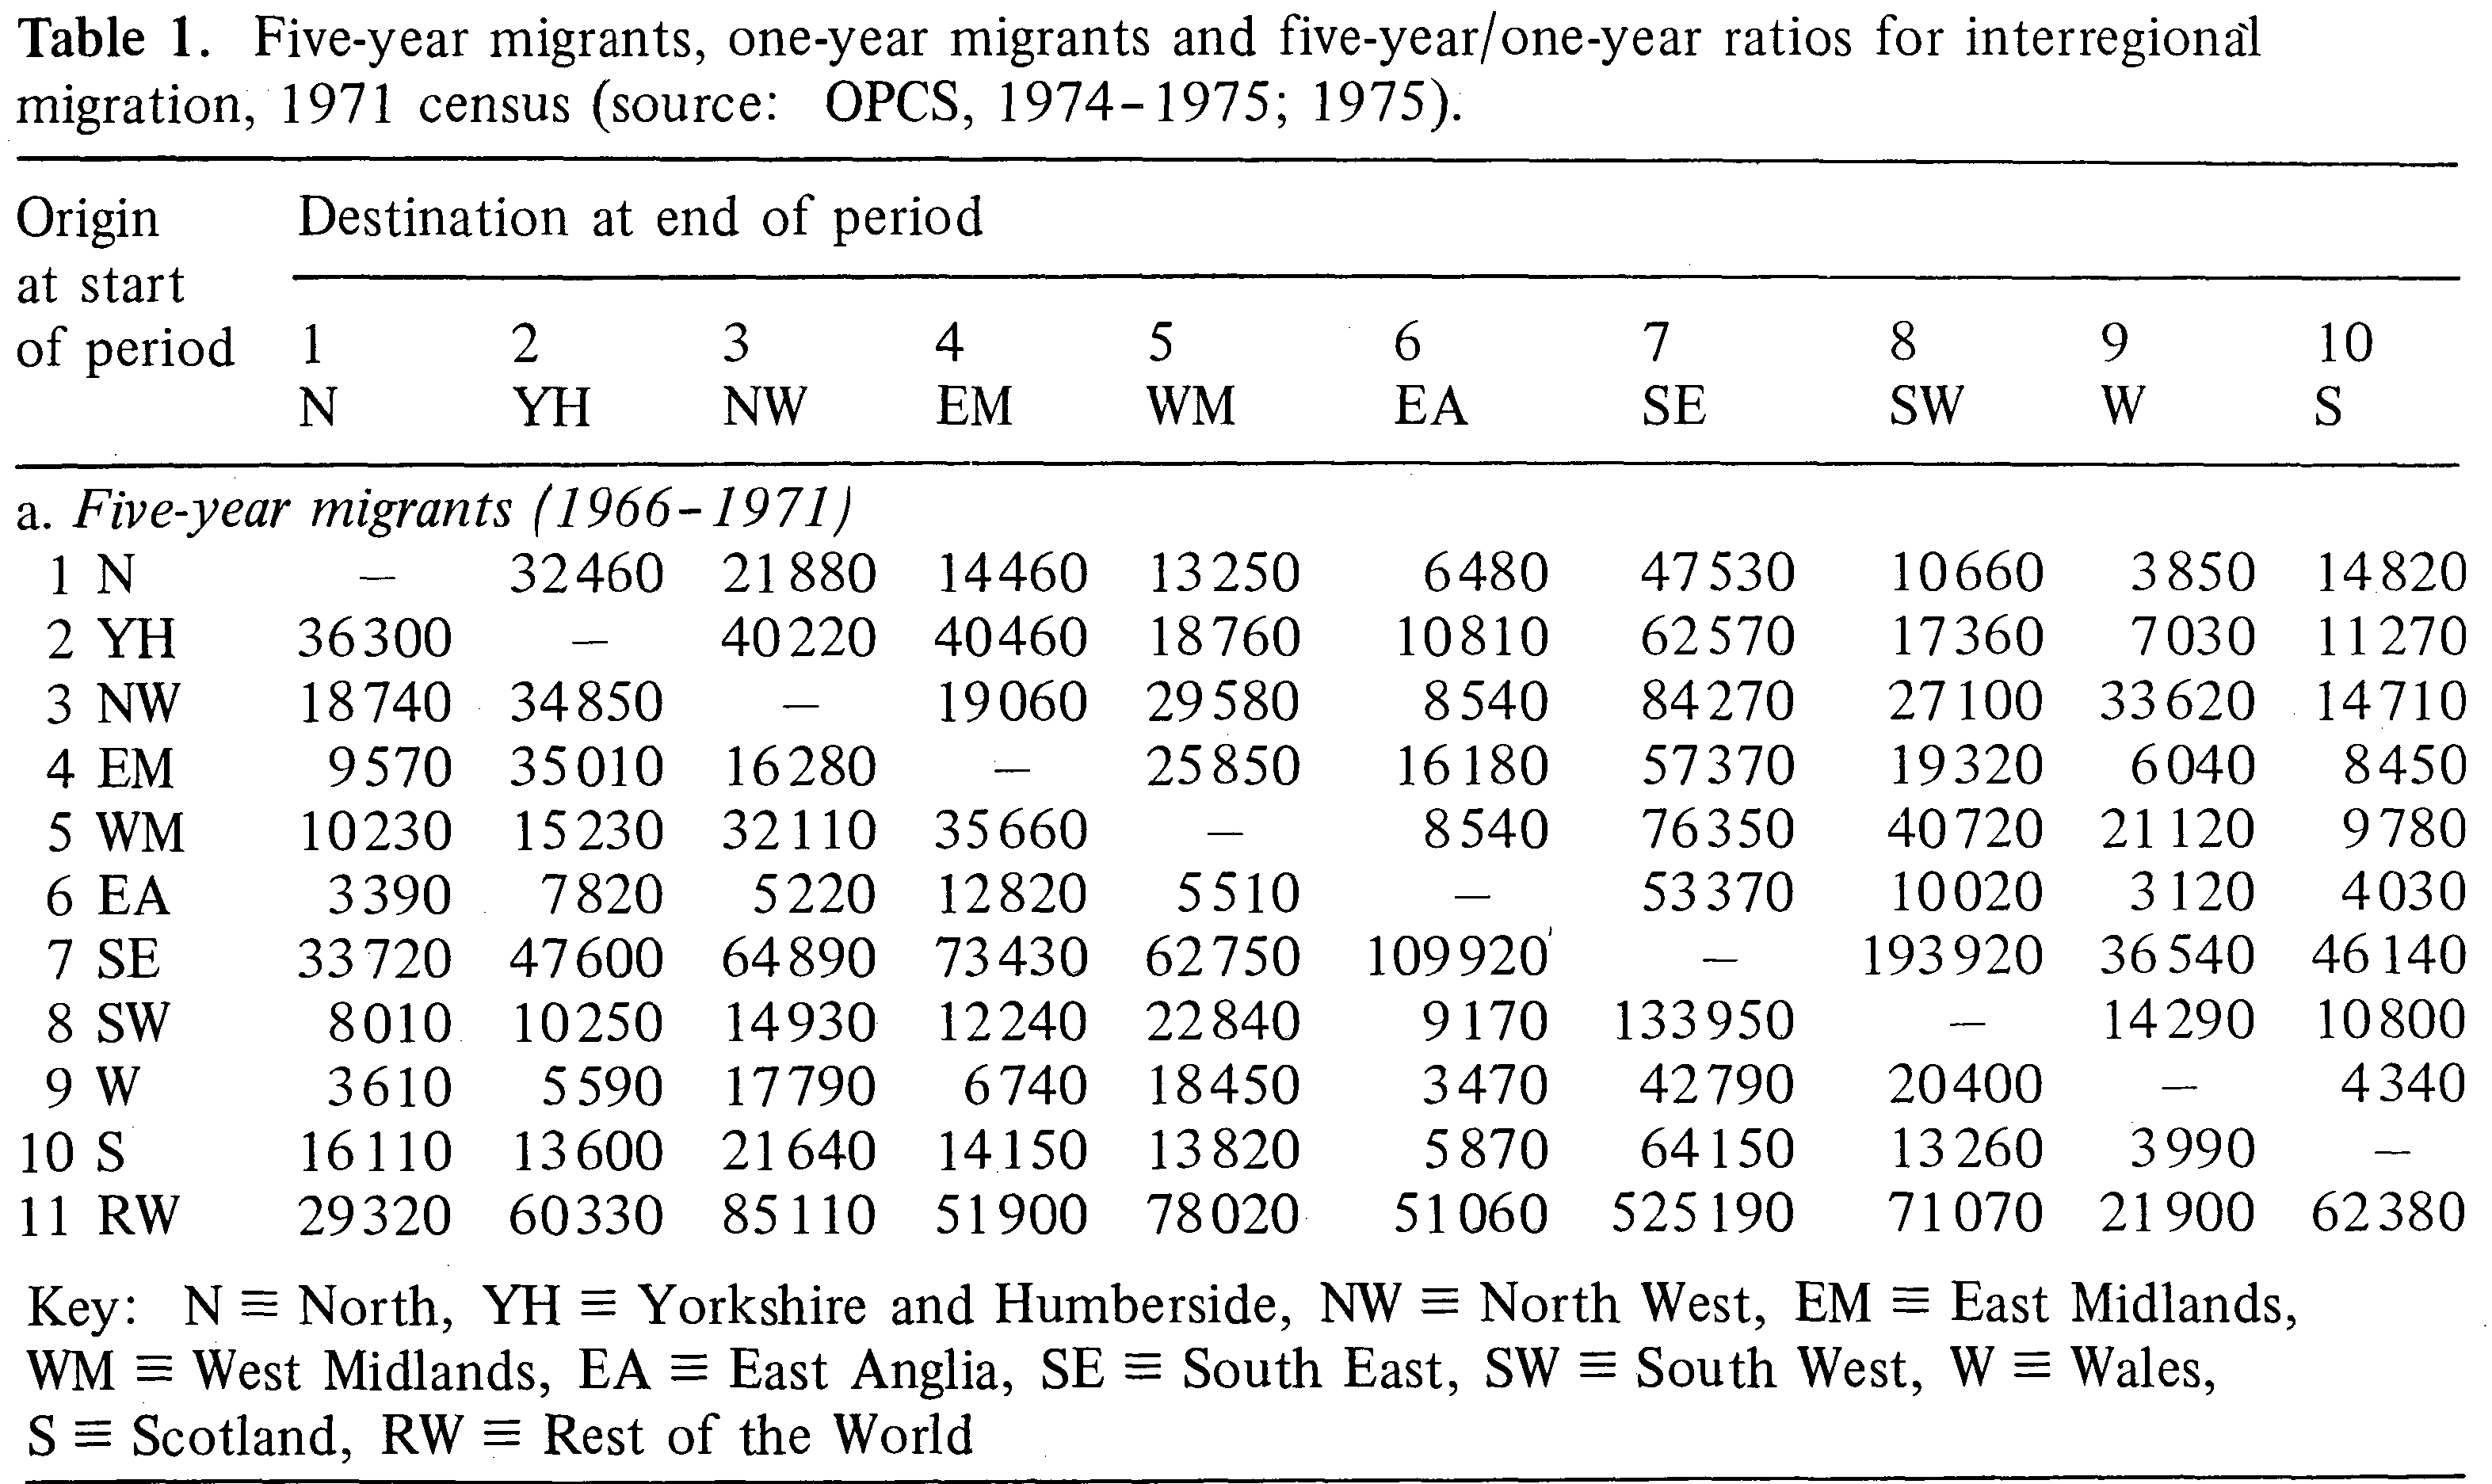
\includegraphics[width=1\linewidth]{img/rees-1977-one-five-a}

\hypertarget{one-year-five-year-problem---rees-1970-1}{%
\subsection{One-Year Five-Year Problem - Rees 1970}\label{one-year-five-year-problem---rees-1970-1}}

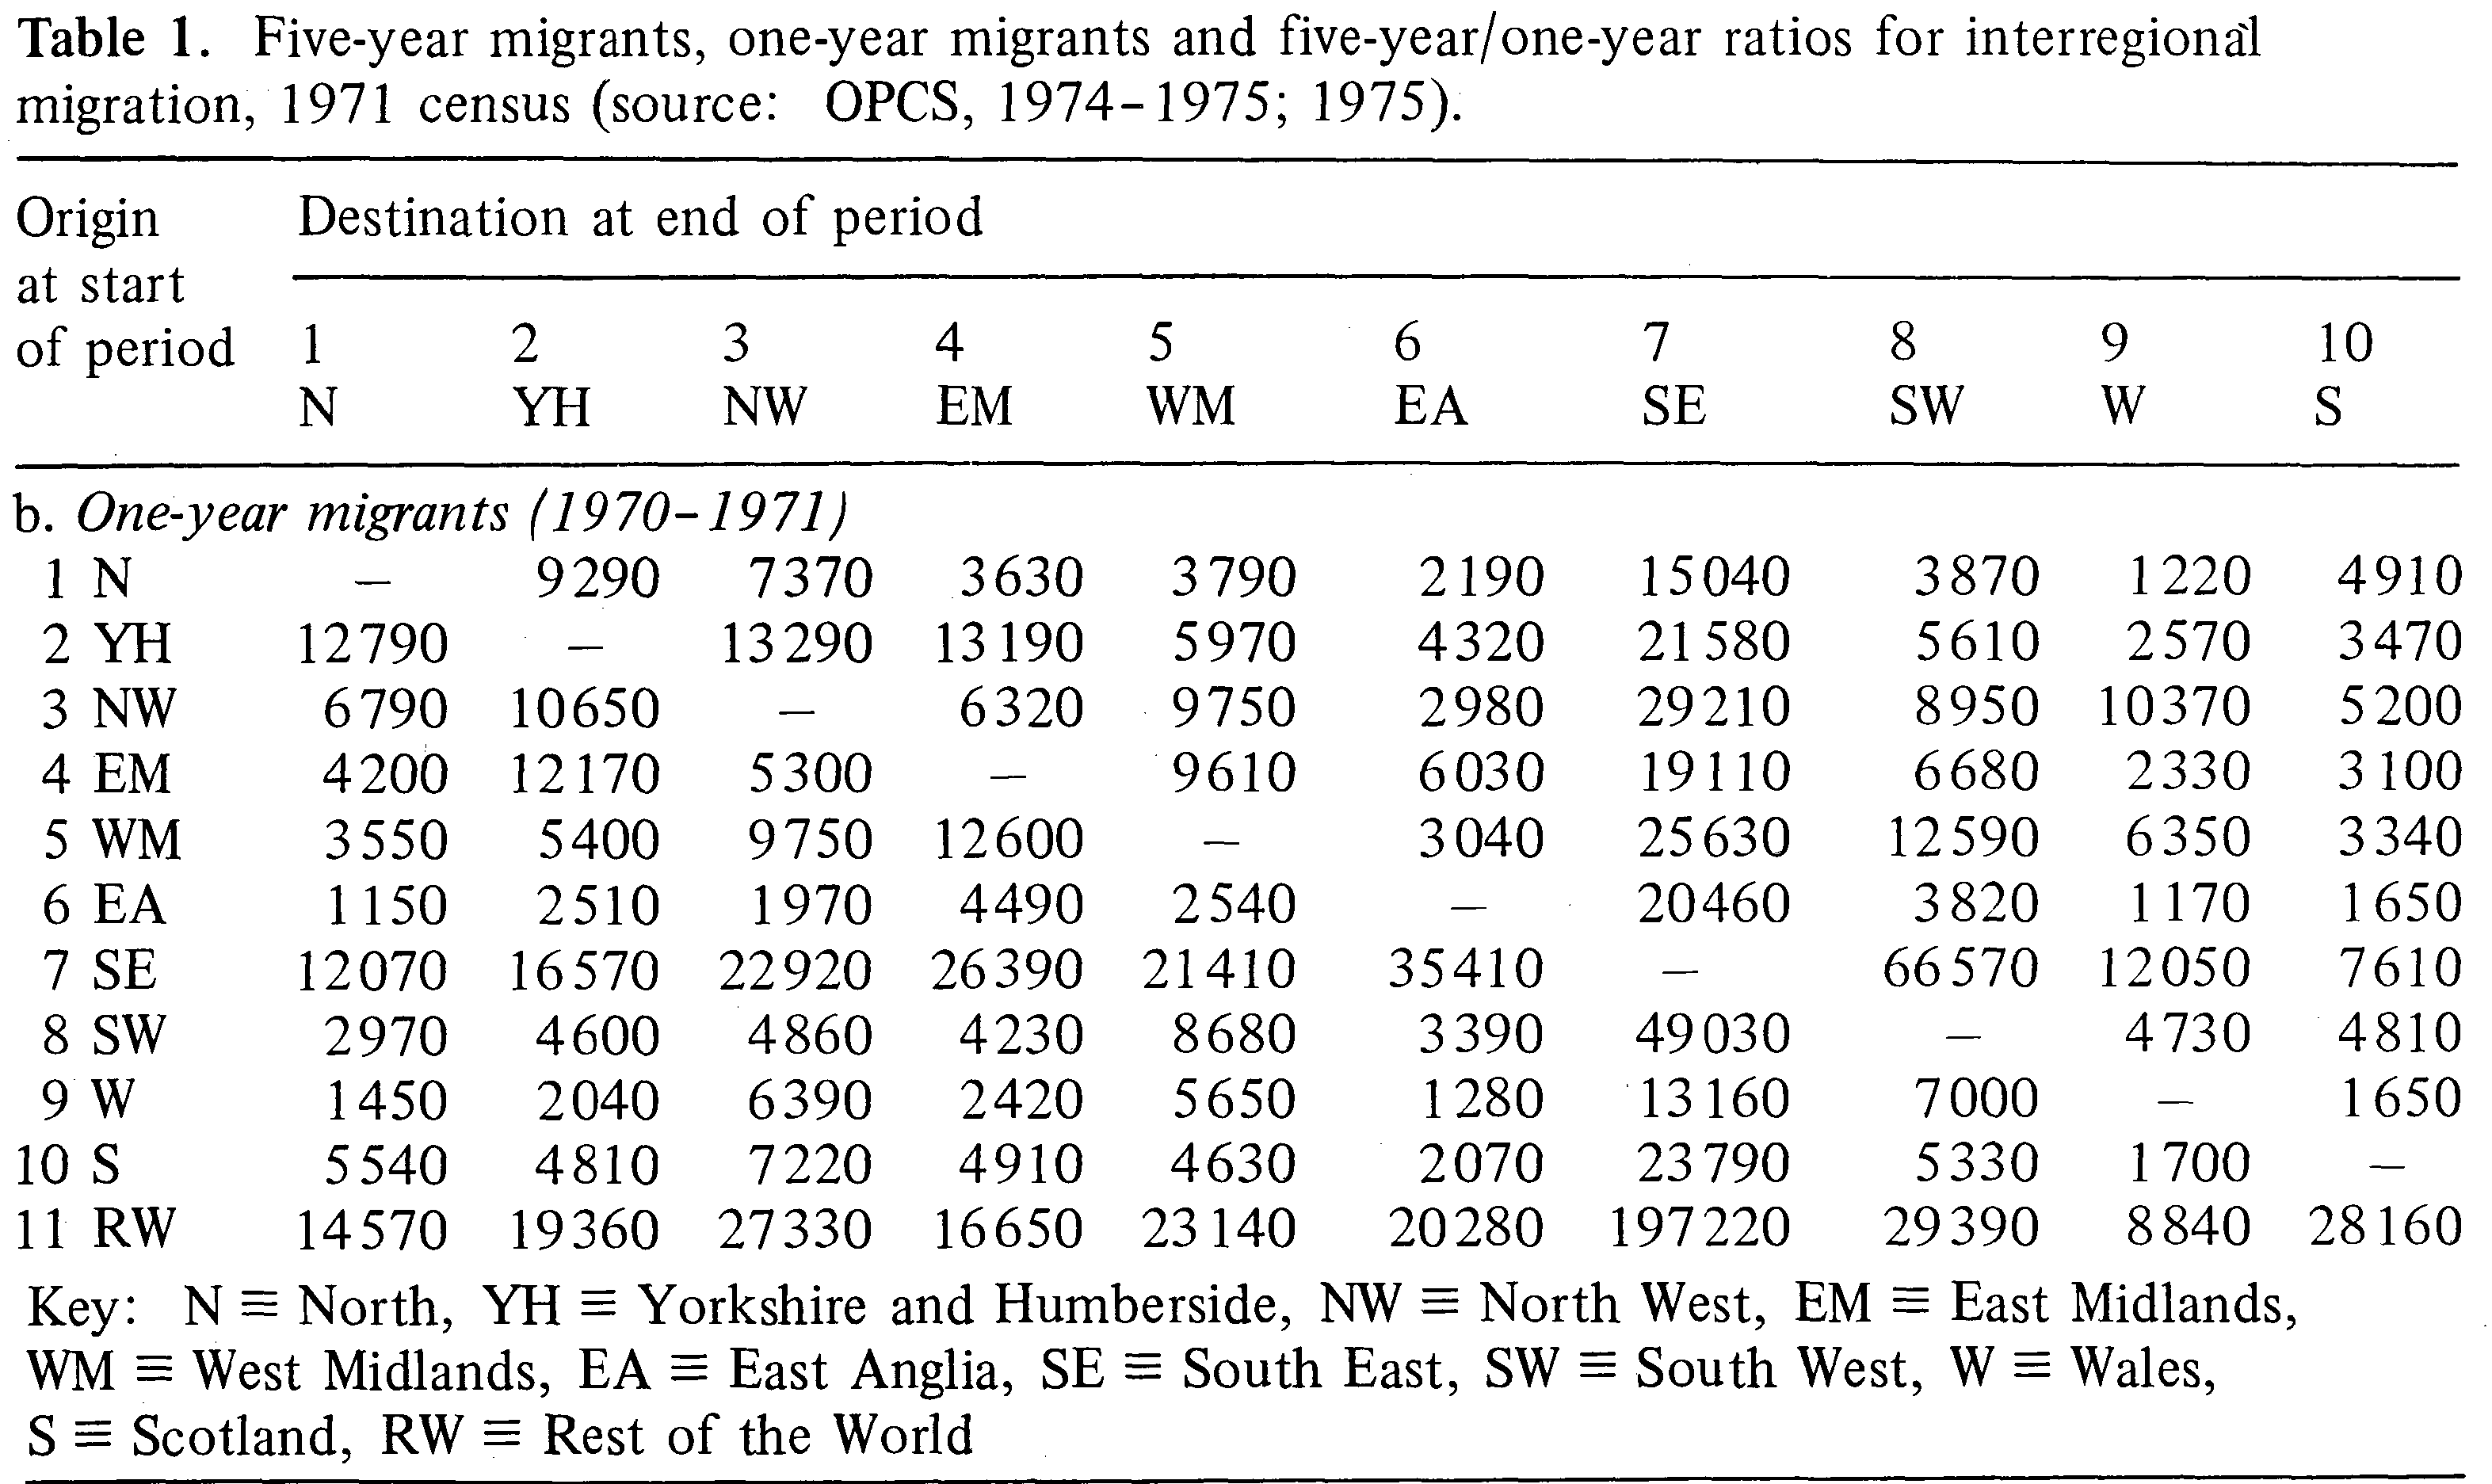
\includegraphics[width=1\linewidth]{img/rees-1977-one-five-b}

\hypertarget{one-year-five-year-problem---rees-1970-2}{%
\subsection{One-Year Five-Year Problem - Rees 1970}\label{one-year-five-year-problem---rees-1970-2}}

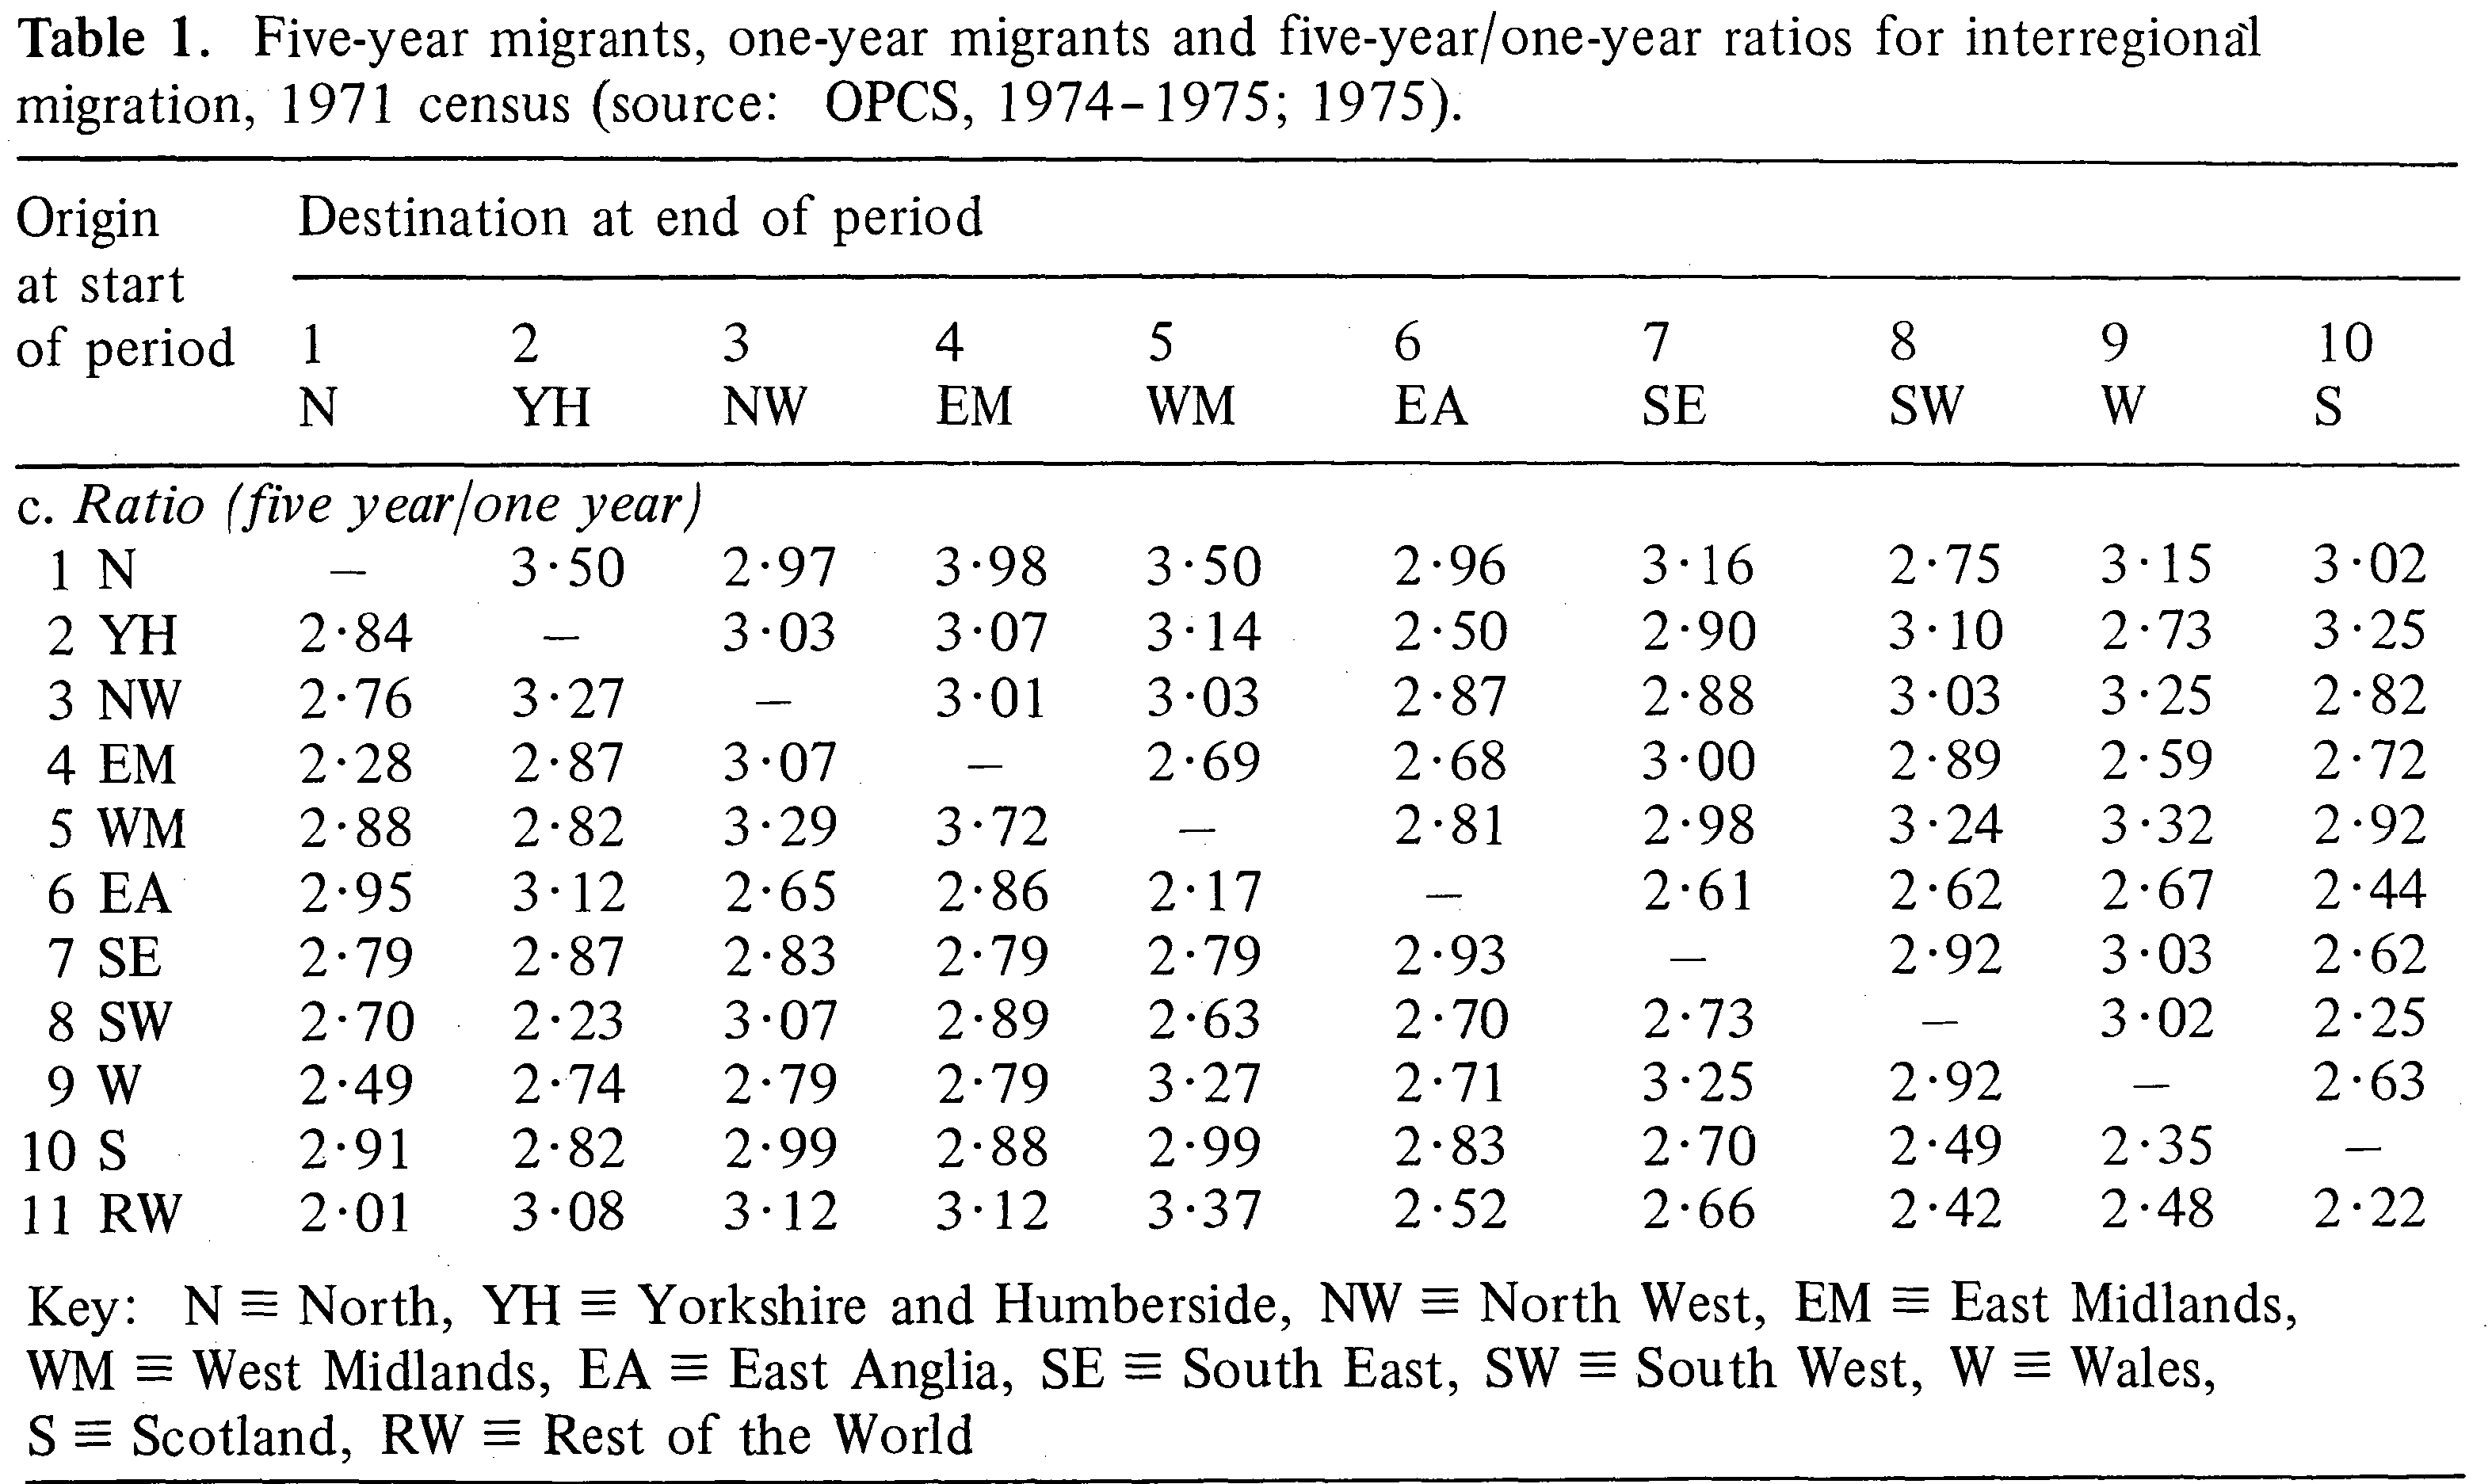
\includegraphics[width=1\linewidth]{img/rees-1977-one-five-c}

\hypertarget{measures}{%
\section{Measures}\label{measures}}

\hypertarget{migration-measures}{%
\subsection{Migration measures}\label{migration-measures}}

\begin{itemize}
\tightlist
\item
  There are a range of migration measures over differing levels of details

  \begin{itemize}
  \tightlist
  \item
    Region to region
  \item
    Region totals
  \item
    System totals (or index measures)
  \end{itemize}
\item
  Measure might have multiple interchangeable names for the same terms.
\end{itemize}

\hypertarget{region-to-region-measures}{%
\subsection{Region to region measures}\label{region-to-region-measures}}

\begin{itemize}
\tightlist
\item
  \emph{Streams} or \emph{bilateral flow} or \emph{origin-destination flow} is the total number of moves made during a given migration interval that have a common area of origin and a common area of destination.
\item
  Data on migrations, or migrants, can be cross-classified by area of origin and area of destination.

  \begin{itemize}
  \tightlist
  \item
    Forms matrix of \(n \times (n-1)\) streams, from area \(i\) to area \(j\) usually written as \(m_{ij}\)
  \end{itemize}
\item
  Contains a set of \(\frac{n(n -1)}{2}\) pairs of streams, each pair representing movements in opposite directions (\(m_{ij}\) and \(m_{ji}\))
\end{itemize}

\hypertarget{region-to-region-measures-1}{%
\subsection{Region to region measures}\label{region-to-region-measures-1}}

\begin{itemize}
\tightlist
\item
  For a pair of streams that are of unequal size there exists a \emph{dominant} streams and \emph{counter-stream} or \emph{reverse} stream
\item
  Sum of the two members of a pair of streams is called \emph{gross interchange}
\item
  Differences between streams and counter-streams for individual pairs of streams, the balances are \emph{net streams}.
\end{itemize}

\hypertarget{region-totals}{%
\subsection{Region totals}\label{region-totals}}

\begin{itemize}
\item
  Every move is an out-migration (emigration) with respect to the area of origin and an in-migration (immigration) with respect to the area of destination.
\item
  Places of origin and destination dictate how describe migrants and migration
\end{itemize}

\begin{longtable}[]{@{}llll@{}}
\toprule
Scale & Area & Event Term & Migrant Term \\
\midrule
\endhead
Internal & Origin & out-migration & out-migrant \\
& Destination & in-migration & in-migrant \\
International & Origin & emigration & emigrant \\
& Destination & immigration & immigrant \\
\bottomrule
\end{longtable}

\hypertarget{region-totals-1}{%
\subsection{Region totals}\label{region-totals-1}}

\begin{itemize}
\tightlist
\item
  Typically in- or out-migration are evaluated for each region
\item
  Data collected or aggregated without reference to place of origin for in-migration totals, or destination for out-migration totals
\item
  Beyond gross migration totals for each region other measures, other summary measures can also be derived
\end{itemize}

\begin{longtable}[]{@{}
  >{\raggedright\arraybackslash}p{(\columnwidth - 2\tabcolsep) * \real{0.38}}
  >{\raggedright\arraybackslash}p{(\columnwidth - 2\tabcolsep) * \real{0.62}}@{}}
\toprule
\begin{minipage}[b]{\linewidth}\raggedright
Term
\end{minipage} & \begin{minipage}[b]{\linewidth}\raggedright
Definition
\end{minipage} \\
\midrule
\endhead
\emph{Gross} migration & All moves or all migrants \\
\emph{Turnover} & Sum of in-migration and out-migration, or of in-migrants and out-migrants. \\
\emph{Net} migration & Balance of movements in opposing directions from difference between in-migration and out-migration for a specific area \\
\bottomrule
\end{longtable}

\hypertarget{region-totals-2}{%
\subsection{Region totals}\label{region-totals-2}}

\begin{itemize}
\tightlist
\item
  Never met a net-migrant
\item
  \citet{rogers1990rnm} \emph{Requiem for net migration}

  \begin{itemize}
  \tightlist
  \item
    Net migration mis-specifies the spatial dynamics generating observed settlement patterns.
  \item
    Obscure regularities in age profiles of migration
  \item
    Net migration rates confound changing migration propensities with changing population stocks.
  \end{itemize}
\end{itemize}

\hypertarget{rate-measures}{%
\subsection{Rate measures}\label{rate-measures}}

\begin{itemize}
\tightlist
\item
  Out-migration or emigration rates calculated by dividing events in a period by exposure population:
  \[
  e^{[t, t +1]} = \frac{E^{[t, t +1]}}{P}k
  \]
  where \(e^{[t, t +1]}\) is the out or emigration rate, \(E\) is the number of out-migrants or emigrants during the period, \(P\) is the population exposed to the likelihood of migration during the period and \(k\) is a constant, usually 1000.
\item
  Exposure population is typically either the

  \begin{itemize}
  \tightlist
  \item
    Population at the mid-interval, under the assumption that migration is uniformly distributed across the interval.
  \item
    Population at the start or end of the interval under the assumption that migration has a negligible effect on population change.
  \end{itemize}
\item
  Can be decomposed by a subset of the population such age and/or sex\\
  \[
  e^{[t, t +1]}_{i} = \frac{E_{i}^{[t, t +1]}}{P_{i}}k
  \]
\end{itemize}

\hypertarget{rates}{%
\subsection{Rates}\label{rates}}

\begin{itemize}
\item
  In-migration or immigration, the population exposed to the risk of migrating into a region is the entire population of the world living elsewhere.
\item
  However, rates calculated by dividing events by the exposure time of the current residents (the population group \textbf{not} exposed to risk).
  \[
  i^{[t, t +1]} = \frac{I^{[t, t +1]}}{P}k
  \]
\item
  Net migration rates, like in-migration rates, are calculated by dividing events by the exposure time of the current residents (the population group \textbf{not} exposed to risk).
  \[
  m^{[t, t +1]} = \frac{M^{[t, t +1]}}{P}k
  \]
\end{itemize}

\hypertarget{rates-1}{%
\subsection{Rates}\label{rates-1}}

\begin{itemize}
\tightlist
\item
  In-migration and net migration rates are unlike other demographic rates.

  \begin{itemize}
  \tightlist
  \item
    Not using the true population at risk in the denominator
  \end{itemize}
\item
  However, using the resident population satisfies the needs of the demographic balancing equation, since rates of gain and loss are measured relative to the same population.
  \[
  \begin{aligned}
  P^{t+1} &=  P^{t} + B^{[t, t +1]} - D^{[t, t +1]} +  M^{[t, t +1]} \\
  P^{t+1} &=  P^{t} \left(1 + b^{[t, t +1]} - d^{[t, t +1]} +  m^{[t, t +1]} \right)\\
  &= P^{t} \left(1 + b^{[t, t +1]} - d^{[t, t +1]} +  i^{[t, t +1]} - e^{[t, t +1]} \right)
  \end{aligned}
  \]
  where we can substitute net migration \(M^{[t, t +1]}\) with difference of in- and out-migration over the period (\(I^{[t, t +1]} - O^{[t, t +1]}\))
  \[
  \begin{aligned}
  P^{t+1}&= P^{t} + B^{[t, t +1]} - D^{[t, t +1]} +  I^{[t, t +1]} - O^{[t, t +1]} \\
  &= P^{t} \left(1 + b^{[t, t +1]} - d^{[t, t +1]} +  i^{[t, t +1]} - o^{[t, t +1]} \right)
  \end{aligned}
  \]
\end{itemize}

\hypertarget{handling-migration-data-in-r}{%
\chapter{Handling Migration Data in R}\label{handling-migration-data-in-r}}

\hypertarget{contingency-table}{%
\section{Contingency Table}\label{contingency-table}}

\hypertarget{contingency-table-1}{%
\subsection{Contingency Table}\label{contingency-table-1}}

\begin{itemize}
\tightlist
\item
  Bilateral migration flow data are commonly represented in square tables.
\item
  Values in non-diagonal cells represent a origin-destination count of migration between a specified set of regions.
\item
  Values in diagonal cells represent some form of non-moving population, or those that move within a region, which are typically not presented.
\end{itemize}

\emph{Origin}

\emph{Destination}

A

B

C

D

Sum

A

100

30

70

200

B

50

45

5

100

C

60

35

40

135

D

20

25

20

65

Sum

130

160

95

115

500

\hypertarget{contingency-table-2}{%
\subsection{Contingency Table}\label{contingency-table-2}}

\begin{itemize}
\tightlist
\item
  Often denoted as \(m_{ij}\)

  \begin{itemize}
  \tightlist
  \item
    Row totals, the out-migration counts: \(\sum_j m_{ij} = m_{i+}\)
  \item
    Column totals, the in-migration counts: \(\sum_i m_{ij} = m_{+j}\)
  \item
    Net migration totals: \(m_{i+} - m_{i+}\)
  \item
    Total migration: \(m_{++}\)
  \end{itemize}
\end{itemize}

\hypertarget{data-manipulation}{%
\section{Data Manipulation}\label{data-manipulation}}

\hypertarget{r-matrix-and-array}{%
\subsection{\texorpdfstring{R \texttt{matrix} and \texttt{array}}{R matrix and array}}\label{r-matrix-and-array}}

\begin{itemize}
\tightlist
\item
  Some functions for describing and estimating migration in R require flow tables as \texttt{matrix} or \texttt{array} type objects
\item
  Create a \texttt{matrix} in R using the \texttt{matrix()} function

  \begin{itemize}
  \tightlist
  \item
    Data read in by column. Change change using \texttt{byrow\ =\ FALSE}
  \item
    Use the \texttt{dimnames} argument to supply region names
  \end{itemize}
\end{itemize}

\begin{Shaded}
\begin{Highlighting}[]
\CommentTok{\# create region labels}
\NormalTok{r }\OtherTok{\textless{}{-}}\NormalTok{ LETTERS[}\DecValTok{1}\SpecialCharTok{:}\DecValTok{4}\NormalTok{]}
\NormalTok{r}
\end{Highlighting}
\end{Shaded}

\begin{verbatim}
## [1] "A" "B" "C" "D"
\end{verbatim}

\begin{Shaded}
\begin{Highlighting}[]
\CommentTok{\# create matrix}
\NormalTok{m0 }\OtherTok{\textless{}{-}} \FunctionTok{matrix}\NormalTok{(}\AttributeTok{data =} \FunctionTok{c}\NormalTok{(}\DecValTok{0}\NormalTok{, }\DecValTok{100}\NormalTok{, }\DecValTok{30}\NormalTok{, }\DecValTok{70}\NormalTok{, }\DecValTok{50}\NormalTok{, }\DecValTok{0}\NormalTok{, }\DecValTok{45}\NormalTok{, }\DecValTok{5}\NormalTok{, }\DecValTok{60}\NormalTok{, }\DecValTok{35}\NormalTok{, }\DecValTok{0}\NormalTok{, }\DecValTok{40}\NormalTok{, }\DecValTok{20}\NormalTok{, }\DecValTok{25}\NormalTok{, }\DecValTok{20}\NormalTok{, }\DecValTok{0}\NormalTok{), }
             \AttributeTok{nrow =} \DecValTok{4}\NormalTok{, }\AttributeTok{ncol =} \DecValTok{4}\NormalTok{, }\AttributeTok{byrow =} \ConstantTok{TRUE}\NormalTok{,}
             \AttributeTok{dimnames =} \FunctionTok{list}\NormalTok{(}\AttributeTok{orig =}\NormalTok{ r, }\AttributeTok{dest =}\NormalTok{ r))}
\NormalTok{m0}
\end{Highlighting}
\end{Shaded}

\begin{verbatim}
##     dest
## orig  A   B  C  D
##    A  0 100 30 70
##    B 50   0 45  5
##    C 60  35  0 40
##    D 20  25 20  0
\end{verbatim}

\hypertarget{r-matrix-and-array-1}{%
\subsection{\texorpdfstring{R \texttt{matrix} and \texttt{array}}{R matrix and array}}\label{r-matrix-and-array-1}}

\begin{itemize}
\tightlist
\item
  Create an \texttt{array} in R using the \texttt{array()} function
\end{itemize}

\begin{Shaded}
\begin{Highlighting}[]
\NormalTok{m1 }\OtherTok{\textless{}{-}} \FunctionTok{array}\NormalTok{(}\AttributeTok{data =} \FunctionTok{sample}\NormalTok{(}\AttributeTok{x =} \DecValTok{1}\SpecialCharTok{:}\DecValTok{100}\NormalTok{, }\AttributeTok{size =} \DecValTok{32}\NormalTok{), }
            \AttributeTok{dim =} \FunctionTok{c}\NormalTok{(}\DecValTok{4}\NormalTok{, }\DecValTok{4}\NormalTok{, }\DecValTok{2}\NormalTok{), }
            \AttributeTok{dimnames =} \FunctionTok{list}\NormalTok{(}\AttributeTok{orig =}\NormalTok{ r, }\AttributeTok{dest =}\NormalTok{ r, }\AttributeTok{sex =} \FunctionTok{c}\NormalTok{(}\StringTok{"female"}\NormalTok{, }\StringTok{"male"}\NormalTok{)))}
\NormalTok{m1}
\end{Highlighting}
\end{Shaded}

\begin{verbatim}
## , , sex = female
## 
##     dest
## orig  A  B  C  D
##    A 88 66 58 75
##    B 33 45 10  5
##    C 24 74 79 29
##    D 77 56 94 37
## 
## , , sex = male
## 
##     dest
## orig  A  B  C  D
##    A 86 16 87 46
##    B 65 54 14  8
##    C 95 63 43 71
##    D 38 91 68 70
\end{verbatim}

\hypertarget{show-totals}{%
\subsection{Show totals}\label{show-totals}}

\begin{itemize}
\tightlist
\item
  The \texttt{addmargins()} functions adds extra row, column and tables to display the dimension sums.
\end{itemize}

\begin{Shaded}
\begin{Highlighting}[]
\FunctionTok{addmargins}\NormalTok{(}\AttributeTok{A =}\NormalTok{ m0)}
\end{Highlighting}
\end{Shaded}

\begin{verbatim}
##      dest
## orig    A   B  C   D Sum
##   A     0 100 30  70 200
##   B    50   0 45   5 100
##   C    60  35  0  40 135
##   D    20  25 20   0  65
##   Sum 130 160 95 115 500
\end{verbatim}

\hypertarget{convert-to-matrix}{%
\subsection{Convert to matrix}\label{convert-to-matrix}}

\begin{itemize}
\tightlist
\item
  Data will not always come as an \texttt{matrix} or an \texttt{array}.
\item
  There a couple of useful functions in R to convert data to when working with migration tables in R
\item
  The \texttt{xtab()} function converts data frames into a \texttt{matrix} or \texttt{array}

  \begin{itemize}
  \tightlist
  \item
    \texttt{formula} column names with

    \begin{itemize}
    \tightlist
    \item
      left hand side the column name to fill the \texttt{matrix} or \texttt{array}
    \item
      a \texttt{\textasciitilde{}} to separate the left and right hand side
    \item
      right hand side the columns to cross-classifying the left hand variable (separated by \texttt{+}).
    \end{itemize}
  \item
    \texttt{data} containing the variables for \texttt{formula}
  \end{itemize}
\item
  The \texttt{as.data.frame.table()} function takes a \texttt{matrix} or \texttt{array} and converts it to a \texttt{data.frame} based on the array dimension names.

  \begin{itemize}
  \tightlist
  \item
    \texttt{responseName} to set the column name of based on the cells of the \texttt{matrix} or \texttt{array}
  \end{itemize}
\end{itemize}

\hypertarget{convert-to-matrix-1}{%
\subsection{Convert to matrix}\label{convert-to-matrix-1}}

\begin{Shaded}
\begin{Highlighting}[]
\CommentTok{\# tidy migration data}
\NormalTok{d0}
\end{Highlighting}
\end{Shaded}

\begin{verbatim}
## # A tibble: 16 x 3
##    orig  dest   flow
##    <chr> <chr> <int>
##  1 A     A         1
##  2 A     B         2
##  3 A     C         3
##  4 A     D         4
##  5 B     A         5
##  6 B     B         6
##  7 B     C         7
##  8 B     D         8
##  9 C     A         9
## 10 C     B        10
## 11 C     C        11
## 12 C     D        12
## 13 D     A        13
## 14 D     B        14
## 15 D     C        15
## 16 D     D        16
\end{verbatim}

\hypertarget{convert-to-matrix-2}{%
\subsection{Convert to matrix}\label{convert-to-matrix-2}}

\begin{Shaded}
\begin{Highlighting}[]
\CommentTok{\# convert to matrix}
\NormalTok{m2 }\OtherTok{\textless{}{-}} \FunctionTok{xtabs}\NormalTok{(}\AttributeTok{formula =}\NormalTok{ flow }\SpecialCharTok{\textasciitilde{}}\NormalTok{ orig }\SpecialCharTok{+}\NormalTok{ dest, }\AttributeTok{data =}\NormalTok{ d0)}
\NormalTok{m2}
\end{Highlighting}
\end{Shaded}

\begin{verbatim}
##     dest
## orig  A  B  C  D
##    A  1  2  3  4
##    B  5  6  7  8
##    C  9 10 11 12
##    D 13 14 15 16
\end{verbatim}

\hypertarget{convert-to-data-frame}{%
\subsection{Convert to data frame}\label{convert-to-data-frame}}

\begin{Shaded}
\begin{Highlighting}[]
\CommentTok{\# convert back to tibble}
\NormalTok{m2 }\SpecialCharTok{\%\textgreater{}\%}
  \FunctionTok{as.data.frame.table}\NormalTok{(}\AttributeTok{responseName =} \StringTok{"flow"}\NormalTok{) }\SpecialCharTok{\%\textgreater{}\%}
  \FunctionTok{as\_tibble}\NormalTok{()}
\end{Highlighting}
\end{Shaded}

\begin{verbatim}
## # A tibble: 16 x 3
##    orig  dest   flow
##    <fct> <fct> <int>
##  1 A     A         1
##  2 B     A         5
##  3 C     A         9
##  4 D     A        13
##  5 A     B         2
##  6 B     B         6
##  7 C     B        10
##  8 D     B        14
##  9 A     C         3
## 10 B     C         7
## 11 C     C        11
## 12 D     C        15
## 13 A     D         4
## 14 B     D         8
## 15 C     D        12
## 16 D     D        16
\end{verbatim}

\hypertarget{convert-to-data-frame-1}{%
\subsection{Convert to data frame}\label{convert-to-data-frame-1}}

\begin{Shaded}
\begin{Highlighting}[]
\CommentTok{\# convert array to tibble}
\NormalTok{d1 }\OtherTok{\textless{}{-}}\NormalTok{ m1 }\SpecialCharTok{\%\textgreater{}\%}
  \FunctionTok{as.data.frame.table}\NormalTok{(}\AttributeTok{responseName =} \StringTok{"flow"}\NormalTok{) }\SpecialCharTok{\%\textgreater{}\%}
  \FunctionTok{as\_tibble}\NormalTok{()}
\NormalTok{d1}
\end{Highlighting}
\end{Shaded}

\begin{verbatim}
## # A tibble: 32 x 4
##    orig  dest  sex     flow
##    <fct> <fct> <fct>  <int>
##  1 A     A     female    88
##  2 B     A     female    33
##  3 C     A     female    24
##  4 D     A     female    77
##  5 A     B     female    66
##  6 B     B     female    45
##  7 C     B     female    74
##  8 D     B     female    56
##  9 A     C     female    58
## 10 B     C     female    10
## # ... with 22 more rows
\end{verbatim}

\hypertarget{matrix-operations}{%
\section{Matrix Operations}\label{matrix-operations}}

\hypertarget{displaying-migration-matrics}{%
\subsection{Displaying migration matrics}\label{displaying-migration-matrics}}

\begin{itemize}
\tightlist
\item
  When dealing with migration \texttt{matrix} objects in R, they often are difficult to view

  \begin{itemize}
  \tightlist
  \item
    Lengthy dimension names,
  \item
    Unit size
  \item
    Diagonal terms included but not of interest
  \end{itemize}
\item
  Some helpful R functions to adapt objects for easier viewing
\item
  Demonstrate with the \texttt{uar\_1960} object in the \emph{migest} package

  \begin{itemize}
  \tightlist
  \item
    Lifetime migration matrix for Governorates of United Arab Republic in 1960 used in the manual of \citet{UnitedNations1983}
  \end{itemize}
\end{itemize}

\hypertarget{displaying-migration-matrics-1}{%
\subsection{Displaying migration matrics}\label{displaying-migration-matrics-1}}

\begin{Shaded}
\begin{Highlighting}[]
\FunctionTok{library}\NormalTok{(migest)}
\NormalTok{uar\_1960}
\end{Highlighting}
\end{Shaded}

\begin{verbatim}
##             dest
## orig           Cairo Alexandria Port-Said Ismailia Kalyubia Gharbia Menoufia
##   Cairo      2079434      31049      5293     9813    23837   10034     7038
##   Alexandria   47220    1085602      2641     2625     2135    4921     1505
##   Port-Said     9464       2562    168046     6461      496     817      323
##   Ismailia      9518       1395      3490   171297      718     910      306
##   Kalyubia     90668       4730       758     3182   886464    3727     3523
##   Gharbia      99179      39953      1742     3347     7870 1604851     6313
##   Menoufia    216764      46781      1640     3338     2918   29580  1308283
##   Giza         64584       4899       513     2013     2887    1503     2161
##   Assyiut     100305      25497      1738     2522      122    2245      636
##   Souhag      100100      63712     12087     9436      295    2791     1095
##   All others  456464     177476     43898    66973    49816   47315    12179
##             dest
## orig            Giza Assyiut  Souhag All others
##   Cairo        88543    4951    2569      58476
##   Alexandria    6910    1355    1467      29534
##   Port-Said     1505     326     454      11184
##   Ismailia      1593     319     263      10269
##   Kalyubia     10279     340     128      18076
##   Gharbia      14529     848     491      64140
##   Menoufia     30915     567     401      47843
##   Giza       1040179     540     433      13518
##   Assyiut      13153 1290255    5955      35157
##   Souhag       17958   11608 1540020      53224
##   All others   94577   14690   22375   11900302
\end{verbatim}

\hypertarget{abbriviate-names}{%
\subsection{Abbriviate names}\label{abbriviate-names}}

\begin{itemize}
\tightlist
\item
  View and alter the \texttt{matrix} dimension names using \texttt{rownames()} and \texttt{colnames()} or \texttt{dimnames()}
\item
  The \texttt{abbreviate()} function applies an algorithm to shorten names
\end{itemize}

\begin{Shaded}
\begin{Highlighting}[]
\FunctionTok{dimnames}\NormalTok{(uar\_1960)}
\end{Highlighting}
\end{Shaded}

\begin{verbatim}
## $orig
##  [1] "Cairo"      "Alexandria" "Port-Said"  "Ismailia"   "Kalyubia"  
##  [6] "Gharbia"    "Menoufia"   "Giza"       "Assyiut"    "Souhag"    
## [11] "All others"
## 
## $dest
##  [1] "Cairo"      "Alexandria" "Port-Said"  "Ismailia"   "Kalyubia"  
##  [6] "Gharbia"    "Menoufia"   "Giza"       "Assyiut"    "Souhag"    
## [11] "All others"
\end{verbatim}

\begin{Shaded}
\begin{Highlighting}[]
\CommentTok{\# make a copy}
\NormalTok{u0 }\OtherTok{\textless{}{-}}\NormalTok{ uar\_1960}
\CommentTok{\# new abbreviated region names}
\NormalTok{r }\OtherTok{\textless{}{-}} \FunctionTok{list}\NormalTok{(}\AttributeTok{orig =}\NormalTok{ uar\_1960 }\SpecialCharTok{\%\textgreater{}\%}
            \FunctionTok{rownames}\NormalTok{() }\SpecialCharTok{\%\textgreater{}\%}
            \FunctionTok{abbreviate}\NormalTok{(),}
          \AttributeTok{dest =}\NormalTok{ uar\_1960 }\SpecialCharTok{\%\textgreater{}\%}
            \FunctionTok{colnames}\NormalTok{() }\SpecialCharTok{\%\textgreater{}\%}
            \FunctionTok{abbreviate}\NormalTok{())}
\end{Highlighting}
\end{Shaded}

\hypertarget{abbriviate-names-1}{%
\subsection{Abbriviate names}\label{abbriviate-names-1}}

\begin{Shaded}
\begin{Highlighting}[]
\NormalTok{r}
\end{Highlighting}
\end{Shaded}

\begin{verbatim}
## $orig
##      Cairo Alexandria  Port-Said   Ismailia   Kalyubia    Gharbia   Menoufia 
##     "Cair"     "Alxn"     "Pr-S"     "Isml"     "Klyb"     "Ghrb"     "Menf" 
##       Giza    Assyiut     Souhag All others 
##     "Giza"     "Assy"     "Sohg"     "Allo" 
## 
## $dest
##      Cairo Alexandria  Port-Said   Ismailia   Kalyubia    Gharbia   Menoufia 
##     "Cair"     "Alxn"     "Pr-S"     "Isml"     "Klyb"     "Ghrb"     "Menf" 
##       Giza    Assyiut     Souhag All others 
##     "Giza"     "Assy"     "Sohg"     "Allo"
\end{verbatim}

\begin{Shaded}
\begin{Highlighting}[]
\CommentTok{\# apply the abbreviated region names}
\FunctionTok{dimnames}\NormalTok{(u0) }\OtherTok{\textless{}{-}}\NormalTok{ r}
\end{Highlighting}
\end{Shaded}

\hypertarget{abbriviate-names-2}{%
\subsection{Abbriviate names}\label{abbriviate-names-2}}

\begin{Shaded}
\begin{Highlighting}[]
\NormalTok{u0}
\end{Highlighting}
\end{Shaded}

\begin{verbatim}
##       dest
## orig      Cair    Alxn   Pr-S   Isml   Klyb    Ghrb    Menf    Giza    Assy
##   Cair 2079434   31049   5293   9813  23837   10034    7038   88543    4951
##   Alxn   47220 1085602   2641   2625   2135    4921    1505    6910    1355
##   Pr-S    9464    2562 168046   6461    496     817     323    1505     326
##   Isml    9518    1395   3490 171297    718     910     306    1593     319
##   Klyb   90668    4730    758   3182 886464    3727    3523   10279     340
##   Ghrb   99179   39953   1742   3347   7870 1604851    6313   14529     848
##   Menf  216764   46781   1640   3338   2918   29580 1308283   30915     567
##   Giza   64584    4899    513   2013   2887    1503    2161 1040179     540
##   Assy  100305   25497   1738   2522    122    2245     636   13153 1290255
##   Sohg  100100   63712  12087   9436    295    2791    1095   17958   11608
##   Allo  456464  177476  43898  66973  49816   47315   12179   94577   14690
##       dest
## orig      Sohg     Allo
##   Cair    2569    58476
##   Alxn    1467    29534
##   Pr-S     454    11184
##   Isml     263    10269
##   Klyb     128    18076
##   Ghrb     491    64140
##   Menf     401    47843
##   Giza     433    13518
##   Assy    5955    35157
##   Sohg 1540020    53224
##   Allo   22375 11900302
\end{verbatim}

\hypertarget{data-scaling}{%
\subsection{Data scaling}\label{data-scaling}}

\begin{itemize}
\tightlist
\item
  Basic arithmetic operators to scale the data to an appropriate level
\item
  The \texttt{round()} function to specify precision of numbers
\end{itemize}

\begin{Shaded}
\begin{Highlighting}[]
\NormalTok{u1 }\OtherTok{\textless{}{-}} \FunctionTok{round}\NormalTok{(}\AttributeTok{x =}\NormalTok{ u0}\SpecialCharTok{/}\DecValTok{1000}\NormalTok{, }\AttributeTok{digits =} \DecValTok{1}\NormalTok{)}
\NormalTok{u1}
\end{Highlighting}
\end{Shaded}

\begin{verbatim}
##       dest
## orig     Cair   Alxn  Pr-S  Isml  Klyb   Ghrb   Menf   Giza   Assy   Sohg
##   Cair 2079.4   31.0   5.3   9.8  23.8   10.0    7.0   88.5    5.0    2.6
##   Alxn   47.2 1085.6   2.6   2.6   2.1    4.9    1.5    6.9    1.4    1.5
##   Pr-S    9.5    2.6 168.0   6.5   0.5    0.8    0.3    1.5    0.3    0.5
##   Isml    9.5    1.4   3.5 171.3   0.7    0.9    0.3    1.6    0.3    0.3
##   Klyb   90.7    4.7   0.8   3.2 886.5    3.7    3.5   10.3    0.3    0.1
##   Ghrb   99.2   40.0   1.7   3.3   7.9 1604.9    6.3   14.5    0.8    0.5
##   Menf  216.8   46.8   1.6   3.3   2.9   29.6 1308.3   30.9    0.6    0.4
##   Giza   64.6    4.9   0.5   2.0   2.9    1.5    2.2 1040.2    0.5    0.4
##   Assy  100.3   25.5   1.7   2.5   0.1    2.2    0.6   13.2 1290.3    6.0
##   Sohg  100.1   63.7  12.1   9.4   0.3    2.8    1.1   18.0   11.6 1540.0
##   Allo  456.5  177.5  43.9  67.0  49.8   47.3   12.2   94.6   14.7   22.4
##       dest
## orig      Allo
##   Cair    58.5
##   Alxn    29.5
##   Pr-S    11.2
##   Isml    10.3
##   Klyb    18.1
##   Ghrb    64.1
##   Menf    47.8
##   Giza    13.5
##   Assy    35.2
##   Sohg    53.2
##   Allo 11900.3
\end{verbatim}

\hypertarget{diagonal-elements}{%
\subsection{Diagonal elements}\label{diagonal-elements}}

\begin{itemize}
\tightlist
\item
  Set diagonal terms (non-movers) to zero using the \texttt{diag()} function
\end{itemize}

\begin{Shaded}
\begin{Highlighting}[]
\NormalTok{u2 }\OtherTok{\textless{}{-}}\NormalTok{ u0}
\FunctionTok{diag}\NormalTok{(u2) }\OtherTok{\textless{}{-}} \DecValTok{0}
\NormalTok{u2}
\end{Highlighting}
\end{Shaded}

\begin{verbatim}
##       dest
## orig     Cair   Alxn  Pr-S  Isml  Klyb  Ghrb  Menf  Giza  Assy  Sohg  Allo
##   Cair      0  31049  5293  9813 23837 10034  7038 88543  4951  2569 58476
##   Alxn  47220      0  2641  2625  2135  4921  1505  6910  1355  1467 29534
##   Pr-S   9464   2562     0  6461   496   817   323  1505   326   454 11184
##   Isml   9518   1395  3490     0   718   910   306  1593   319   263 10269
##   Klyb  90668   4730   758  3182     0  3727  3523 10279   340   128 18076
##   Ghrb  99179  39953  1742  3347  7870     0  6313 14529   848   491 64140
##   Menf 216764  46781  1640  3338  2918 29580     0 30915   567   401 47843
##   Giza  64584   4899   513  2013  2887  1503  2161     0   540   433 13518
##   Assy 100305  25497  1738  2522   122  2245   636 13153     0  5955 35157
##   Sohg 100100  63712 12087  9436   295  2791  1095 17958 11608     0 53224
##   Allo 456464 177476 43898 66973 49816 47315 12179 94577 14690 22375     0
\end{verbatim}

\hypertarget{summaries}{%
\section{Summaries}\label{summaries}}

\hypertarget{net-flows-and-counterflows}{%
\subsection{Net flows and counterflows}\label{net-flows-and-counterflows}}

\begin{itemize}
\tightlist
\item
  The \emph{migest} package contains a number of functions to provide summaries of origin-destination migration data
\item
  The \texttt{counter()} function calculates the counter flow and net flow

  \begin{itemize}
  \tightlist
  \item
    Accepts \texttt{matrix} or \texttt{data.frame} (or \texttt{tibble}) inputs
  \end{itemize}
\end{itemize}

\begin{Shaded}
\begin{Highlighting}[]
\FunctionTok{counter}\NormalTok{(m0)}
\end{Highlighting}
\end{Shaded}

\begin{verbatim}
## # A tibble: 12 x 7
##    orig  dest  corridor pair   flow counter_flow net_flow
##    <chr> <chr> <chr>    <chr> <dbl>        <dbl>    <dbl>
##  1 B     A     B -> A   A - B    50          100      -50
##  2 C     A     C -> A   A - C    60           30       30
##  3 D     A     D -> A   A - D    20           70      -50
##  4 A     B     A -> B   A - B   100           50       50
##  5 C     B     C -> B   B - C    35           45      -10
##  6 D     B     D -> B   B - D    25            5       20
##  7 A     C     A -> C   A - C    30           60      -30
##  8 B     C     B -> C   B - C    45           35       10
##  9 D     C     D -> C   C - D    20           40      -20
## 10 A     D     A -> D   A - D    70           20       50
## 11 B     D     B -> D   B - D     5           25      -20
## 12 C     D     C -> D   C - D    40           20       20
\end{verbatim}

\hypertarget{net-flows-and-counterflows-1}{%
\subsection{Net flows and counterflows}\label{net-flows-and-counterflows-1}}

\begin{Shaded}
\begin{Highlighting}[]
\NormalTok{d1 }\SpecialCharTok{\%\textgreater{}\%}
  \FunctionTok{group\_by}\NormalTok{(sex) }\SpecialCharTok{\%\textgreater{}\%}
  \FunctionTok{counter}\NormalTok{()}
\end{Highlighting}
\end{Shaded}

\begin{verbatim}
## # A tibble: 24 x 8
## # Groups:   sex [2]
##    orig  dest  corridor pair  sex     flow counter_flow net_flow
##    <chr> <chr> <chr>    <chr> <fct>  <int>        <int>    <int>
##  1 B     A     B -> A   A - B female    33           66      -33
##  2 C     A     C -> A   A - C female    24           58      -34
##  3 D     A     D -> A   A - D female    77           75        2
##  4 A     B     A -> B   A - B female    66           33       33
##  5 C     B     C -> B   B - C female    74           10       64
##  6 D     B     D -> B   B - D female    56            5       51
##  7 A     C     A -> C   A - C female    58           24       34
##  8 B     C     B -> C   B - C female    10           74      -64
##  9 D     C     D -> C   C - D female    94           29       65
## 10 A     D     A -> D   A - D female    75           77       -2
## # ... with 14 more rows
\end{verbatim}

\hypertarget{totals}{%
\subsection{Totals}\label{totals}}

\begin{itemize}
\tightlist
\item
  The \texttt{sum\_turnover()} provides summary in-migration, out-migration, net-migration and turnover totals for each region

  \begin{itemize}
  \tightlist
  \item
    Accepts \texttt{matrix} or \texttt{data.frame} (or \texttt{tibble}) inputs
  \item
    Setting \texttt{type\ =\ "international"} to change labels in outputs
  \end{itemize}
\end{itemize}

\begin{Shaded}
\begin{Highlighting}[]
\FunctionTok{sum\_turnover}\NormalTok{(m0)}
\end{Highlighting}
\end{Shaded}

\begin{verbatim}
## # A tibble: 4 x 5
##   region in_mig out_mig  turn   net
##   <chr>   <dbl>   <dbl> <dbl> <dbl>
## 1 A         130     200   330   -70
## 2 B         160     100   260    60
## 3 C          95     135   230   -40
## 4 D         115      65   180    50
\end{verbatim}

\hypertarget{totals-1}{%
\subsection{Totals}\label{totals-1}}

\begin{Shaded}
\begin{Highlighting}[]
\FunctionTok{sum\_turnover}\NormalTok{(}\AttributeTok{m =}\NormalTok{ d0, }\AttributeTok{type =} \StringTok{"international"}\NormalTok{)}
\end{Highlighting}
\end{Shaded}

\begin{verbatim}
## # A tibble: 4 x 5
##   country   imm   emi  turn   net
##   <chr>   <dbl> <dbl> <dbl> <dbl>
## 1 A          27     9    36    18
## 2 B          26    20    46     6
## 3 C          25    31    56    -6
## 4 D          24    42    66   -18
\end{verbatim}

\hypertarget{totals-2}{%
\subsection{Totals}\label{totals-2}}

\begin{itemize}
\tightlist
\item
  The \texttt{sum\_turnover()} function can be applied with to large data sets spanning multiple years (groups)
\item
  Demonstrate using international flow estimates of \citet{Abel2019}
\end{itemize}

\begin{Shaded}
\begin{Highlighting}[]
\CommentTok{\# read data from web depository}
\NormalTok{f }\OtherTok{\textless{}{-}} \FunctionTok{read\_csv}\NormalTok{(}\StringTok{"https://ndownloader.figshare.com/files/26239945"}\NormalTok{)}
\NormalTok{f}
\end{Highlighting}
\end{Shaded}

\begin{verbatim}
## # A tibble: 235,236 x 9
##    year0 orig  dest  sd_drop_neg sd_rev_neg mig_rate da_min_open da_min_closed
##    <dbl> <chr> <chr>       <dbl>      <dbl>    <dbl>       <dbl>         <dbl>
##  1  1990 BDI   BDI             0          0        0           0             0
##  2  1990 COM   BDI             0          0        0           0             0
##  3  1990 DJI   BDI             0          0        0           0             0
##  4  1990 ERI   BDI             0          0        0           0             0
##  5  1990 ETH   BDI             0          0        0           0             0
##  6  1990 KEN   BDI            30         30       69          45            29
##  7  1990 MDG   BDI             0          0        0           0             0
##  8  1990 MWI   BDI             0          0        0           0             0
##  9  1990 MUS   BDI             0          0        0           0             1
## 10  1990 MYT   BDI             0          0        0           0             0
## # ... with 235,226 more rows, and 1 more variable: da_pb_closed <dbl>
\end{verbatim}

\hypertarget{totals-3}{%
\subsection{Totals}\label{totals-3}}

\begin{Shaded}
\begin{Highlighting}[]
\CommentTok{\# single period}
\NormalTok{f }\SpecialCharTok{\%\textgreater{}\%} 
  \FunctionTok{filter}\NormalTok{(year0 }\SpecialCharTok{==} \DecValTok{1990}\NormalTok{) }\SpecialCharTok{\%\textgreater{}\%}
  \FunctionTok{sum\_turnover}\NormalTok{(}\AttributeTok{flow\_col =} \StringTok{"da\_pb\_closed"}\NormalTok{, }\AttributeTok{type =} \StringTok{"international"}\NormalTok{)}
\end{Highlighting}
\end{Shaded}

\begin{verbatim}
## # A tibble: 197 x 5
##    country     imm    emi    turn     net
##    <chr>     <dbl>  <dbl>   <dbl>   <dbl>
##  1 BDI       61630 381611  443241 -319981
##  2 COM        9009  12011   21020   -3002
##  3 DJI       10949  55945   66894  -44996
##  4 ERI       14633 329383  344016 -314750
##  5 ETH     1635513 177334 1812847 1458179
##  6 KEN      306517  84833  391350  221684
##  7 MDG        9706  19159   28865   -9453
##  8 MWI      112416 974278 1086694 -861862
##  9 MUS       16862  22475   39337   -5613
## 10 MYT       13763   3021   16784   10742
## # ... with 187 more rows
\end{verbatim}

\hypertarget{totals-4}{%
\subsection{Totals}\label{totals-4}}

\begin{Shaded}
\begin{Highlighting}[]
\CommentTok{\# all periods using group\_by}
\NormalTok{f }\SpecialCharTok{\%\textgreater{}\%} 
  \FunctionTok{group\_by}\NormalTok{(year0) }\SpecialCharTok{\%\textgreater{}\%}
  \FunctionTok{sum\_turnover}\NormalTok{(}\AttributeTok{flow\_col =} \StringTok{"da\_pb\_closed"}\NormalTok{, }\AttributeTok{type =} \StringTok{"international"}\NormalTok{) }\SpecialCharTok{\%\textgreater{}\%}
  \FunctionTok{arrange}\NormalTok{(country)}
\end{Highlighting}
\end{Shaded}

\begin{verbatim}
## Adding missing grouping variables: `year0`
\end{verbatim}

\begin{verbatim}
## # A tibble: 1,188 x 6
## # Groups:   year0 [6]
##    year0 country     imm     emi    turn      net
##    <dbl> <chr>     <dbl>   <dbl>   <dbl>    <dbl>
##  1  1990 ABW       15874    1662   17536    14212
##  2  1995 ABW       10945    4007   14952     6938
##  3  2000 ABW       10064    3814   13878     6250
##  4  2005 ABW        7124    7544   14668     -420
##  5  2010 ABW        9910    8654   18564     1256
##  6  2015 ABW       17316   16306   33622     1010
##  7  1990 AFG     3421712  345255 3766967  3076457
##  8  1995 AFG      418906 1286436 1705342  -867530
##  9  2000 AFG     1178865  434706 1613571   744159
## 10  2005 AFG      457339 1500149 1957488 -1042810
## # ... with 1,178 more rows
\end{verbatim}

\hypertarget{rest-of-categroies}{%
\subsection{Rest of categroies}\label{rest-of-categroies}}

\begin{itemize}
\tightlist
\item
  The \texttt{sum\_lump()} function can be used to aggregate up smaller regions.

  \begin{itemize}
  \tightlist
  \item
    Specify the the desired level of small flows using the \texttt{threshold} argument
  \item
    Specify the \texttt{lump} argument to apply the \texttt{threshold} argument to either the \texttt{flow} values or the \texttt{in} and \texttt{out} totals.
  \end{itemize}
\end{itemize}

\begin{Shaded}
\begin{Highlighting}[]
\NormalTok{m0}
\end{Highlighting}
\end{Shaded}

\begin{verbatim}
##     dest
## orig  A   B  C  D
##    A  0 100 30 70
##    B 50   0 45  5
##    C 60  35  0 40
##    D 20  25 20  0
\end{verbatim}

\begin{Shaded}
\begin{Highlighting}[]
\CommentTok{\# threshold on flows (default)}
\FunctionTok{sum\_lump}\NormalTok{(m0, }\AttributeTok{threshold =} \DecValTok{50}\NormalTok{)}
\end{Highlighting}
\end{Shaded}

\begin{verbatim}
## # A tibble: 5 x 3
##   orig  dest   flow
##   <chr> <chr> <dbl>
## 1 A     B       100
## 2 A     D        70
## 3 B     A        50
## 4 C     A        60
## 5 other other   220
\end{verbatim}

\hypertarget{rest-of-categroies-1}{%
\subsection{Rest of categroies}\label{rest-of-categroies-1}}

\begin{Shaded}
\begin{Highlighting}[]
\FunctionTok{addmargins}\NormalTok{(m0)}
\end{Highlighting}
\end{Shaded}

\begin{verbatim}
##      dest
## orig    A   B  C   D Sum
##   A     0 100 30  70 200
##   B    50   0 45   5 100
##   C    60  35  0  40 135
##   D    20  25 20   0  65
##   Sum 130 160 95 115 500
\end{verbatim}

\begin{Shaded}
\begin{Highlighting}[]
\CommentTok{\# threshold on in and out totals}
\FunctionTok{sum\_lump}\NormalTok{(m0, }\AttributeTok{threshold =} \DecValTok{120}\NormalTok{, }\AttributeTok{lump =} \FunctionTok{c}\NormalTok{(}\StringTok{"in"}\NormalTok{, }\StringTok{"out"}\NormalTok{))}
\end{Highlighting}
\end{Shaded}

\begin{verbatim}
## # A tibble: 9 x 3
##   orig  dest   flow
##   <chr> <chr> <dbl>
## 1 A     A         0
## 2 A     C        30
## 3 A     other   170
## 4 B     A        50
## 5 B     C        45
## 6 B     other     5
## 7 other A        80
## 8 other C        20
## 9 other other   100
\end{verbatim}

\hypertarget{rest-of-categroies-2}{%
\subsection{Rest of categroies}\label{rest-of-categroies-2}}

\begin{itemize}
\tightlist
\item
  Useful to reduce the number of corridors when plotting large data sets:
\end{itemize}

\begin{Shaded}
\begin{Highlighting}[]
\CommentTok{\# add continental regions to the global flow data set}
\FunctionTok{library}\NormalTok{(countrycode)}
\NormalTok{d }\OtherTok{\textless{}{-}}\NormalTok{ f }\SpecialCharTok{\%\textgreater{}\%} 
  \FunctionTok{filter}\NormalTok{(year0 }\SpecialCharTok{==} \DecValTok{2015}\NormalTok{) }\SpecialCharTok{\%\textgreater{}\%}
  \FunctionTok{mutate}\NormalTok{(}
    \AttributeTok{orig\_reg =} 
      \FunctionTok{countrycode}\NormalTok{(}\AttributeTok{sourcevar =}\NormalTok{ orig, }\AttributeTok{origin =} \StringTok{"iso3c"}\NormalTok{, }\AttributeTok{dest =} \StringTok{"un.region.name"}\NormalTok{),}
    \AttributeTok{dest\_reg =} 
      \FunctionTok{countrycode}\NormalTok{(}\AttributeTok{sourcevar =}\NormalTok{ dest, }\AttributeTok{origin =} \StringTok{"iso3c"}\NormalTok{, }\AttributeTok{dest =} \StringTok{"un.region.name"}\NormalTok{)) }\SpecialCharTok{\%\textgreater{}\%}
  \FunctionTok{relocate}\NormalTok{(}\FunctionTok{contains}\NormalTok{(}\StringTok{"orig"}\NormalTok{), }\FunctionTok{contains}\NormalTok{(}\StringTok{"dest"}\NormalTok{))}
\NormalTok{d}
\end{Highlighting}
\end{Shaded}

\begin{verbatim}
## # A tibble: 40,000 x 11
##    orig  orig_reg dest  dest_reg year0 sd_drop_neg sd_rev_neg mig_rate
##    <chr> <chr>    <chr> <chr>    <dbl>       <dbl>      <dbl>    <dbl>
##  1 BDI   Africa   BDI   Africa    2015           0          0        0
##  2 COM   Africa   BDI   Africa    2015           0          0        0
##  3 DJI   Africa   BDI   Africa    2015           0          0        0
##  4 ERI   Africa   BDI   Africa    2015           0        131        0
##  5 ETH   Africa   BDI   Africa    2015           0         14        0
##  6 KEN   Africa   BDI   Africa    2015         194        194      211
##  7 MDG   Africa   BDI   Africa    2015           0          0        0
##  8 MWI   Africa   BDI   Africa    2015           0          0        0
##  9 MUS   Africa   BDI   Africa    2015           0          0        0
## 10 MYT   Africa   BDI   Africa    2015           0          0        0
## # ... with 39,990 more rows, and 3 more variables: da_min_open <dbl>,
## #   da_min_closed <dbl>, da_pb_closed <dbl>
\end{verbatim}

\hypertarget{rest-of-categroies-3}{%
\subsection{Rest of categroies}\label{rest-of-categroies-3}}

\begin{itemize}
\tightlist
\item
  Apply the \texttt{sum\_lump()} function to lump together smaller flows (less than 100,000) within and between continents.
\end{itemize}

\begin{Shaded}
\begin{Highlighting}[]
\NormalTok{d }\SpecialCharTok{\%\textgreater{}\%}
  \FunctionTok{group\_by}\NormalTok{(orig\_reg, dest\_reg) }\SpecialCharTok{\%\textgreater{}\%}
  \FunctionTok{sum\_lump}\NormalTok{(}\AttributeTok{threshold =} \FloatTok{1e5}\NormalTok{, }\AttributeTok{flow\_col =} \StringTok{"da\_pb\_closed"}\NormalTok{)}
\end{Highlighting}
\end{Shaded}

\begin{verbatim}
## # A tibble: 221 x 5
## # Groups:   orig_reg, dest_reg [36]
##    orig_reg dest_reg orig  dest     flow
##    <chr>    <chr>    <chr> <chr>   <dbl>
##  1 Africa   Africa   BFA   CIV    329531
##  2 Africa   Africa   CAF   COD    163440
##  3 Africa   Africa   CIV   BFA    260320
##  4 Africa   Africa   CIV   MLI    107902
##  5 Africa   Africa   COD   UGA    111439
##  6 Africa   Africa   MLI   CIV    138475
##  7 Africa   Africa   MOZ   ZAF    112554
##  8 Africa   Africa   other other 5091888
##  9 Africa   Africa   SDN   SSD    380532
## 10 Africa   Africa   SDN   TCD    121964
## # ... with 211 more rows
\end{verbatim}

\hypertarget{exercise-ex2.r}{%
\subsection{Exercise (ex2.R)}\label{exercise-ex2.r}}

\begin{Shaded}
\begin{Highlighting}[]
\CommentTok{\# 0.  a) Load the KOSTAT2021.Rproj file. }
\CommentTok{\#     Run the getwd() below. It should print the directory where the }
\CommentTok{\#     KOSTAT2021.Rproj file is located.}
\FunctionTok{getwd}\NormalTok{()}
\CommentTok{\#     b) Load the packages used in this exercise}
\FunctionTok{library}\NormalTok{(tidyverse)}
\FunctionTok{library}\NormalTok{(migest)}
\DocumentationTok{\#\#}
\DocumentationTok{\#\#}
\DocumentationTok{\#\#}
\CommentTok{\# 1. Run the code below to read in the bilateral data in uk\_census\_2011\_tidy.csv }
\CommentTok{\#    from the ONS 2011 British Census}
\NormalTok{uk }\OtherTok{\textless{}{-}} \FunctionTok{read\_csv}\NormalTok{(}\StringTok{"./data/uk\_census\_2011\_tidy.csv"}\NormalTok{)}
\NormalTok{uk}
\CommentTok{\# 2. Create a 12 by 12 origin{-}destination matrix m based on the bilateral flows}
\CommentTok{\#    given in data frame uk}
\NormalTok{m }\OtherTok{\textless{}{-}} \DocumentationTok{\#\#\#\#\#(formula = flow \textasciitilde{} orig + \#\#\#\#\#, data = \#\#\#\#\#)}
\NormalTok{m}
\CommentTok{\# 3. Print the matrix m again, this time include the in{-} and out{-}migration }
\CommentTok{\#    sum totals}
\DocumentationTok{\#\#\#\#\#(m1)}
\CommentTok{\# 4. Create a 12 by 12 by 2 sex{-}specific origin{-}destination array based on the}
\CommentTok{\#    bilateral flows given in data frame uk}
\NormalTok{s }\OtherTok{\textless{}{-}} \DocumentationTok{\#\#\#\#\#(formula = \#\#\#\#\# \textasciitilde{} \#\#\#\#\# + dest + \#\#\#\#\#, data = uk)}
\NormalTok{s}
\CommentTok{\# 5. Run the code below to check that s has 12 x 12 x 2 dimensions}
\FunctionTok{dim}\NormalTok{(s)}
\CommentTok{\# 6. Convert object s from above into a tibble with four columns, orig, dest, }
\CommentTok{\#    sex and flow}
\NormalTok{d }\OtherTok{\textless{}{-}}\NormalTok{ s }\SpecialCharTok{\%\textgreater{}\%}
  \DocumentationTok{\#\#\#\#\#(responseName = "\#\#\#\#\#") \%\textgreater{}\%}
  \DocumentationTok{\#\#\#\#\#()}
\NormalTok{d}
\CommentTok{\# 7. Calculate the counter{-}flow and net{-}flow for each migration pair in the }
\CommentTok{\#    matrix m. Use the arrange() function to show the top 10 migration corridors}
\CommentTok{\#    with biggest net losses }
\NormalTok{m }\SpecialCharTok{\%\textgreater{}\%}
  \DocumentationTok{\#\#\#\#\#() \%\textgreater{}\%}
  \FunctionTok{arrange}\NormalTok{(net\_flow)}
\CommentTok{\# 8. Calculate the sex{-}specific in{-}migration, out{-}migration, turnover and net }
\CommentTok{\#    migration totals for each origin in s. Arrange the results by the smallest}
\CommentTok{\#    turnover totals}
\NormalTok{s }\SpecialCharTok{\%\textgreater{}\%}
  \DocumentationTok{\#\#\#\#\#(responseName = "flow") \%\textgreater{}\%}
  \FunctionTok{group\_by}\NormalTok{(}\DocumentationTok{\#\#\#\#\#) \%\textgreater{}\%}
  \DocumentationTok{\#\#\#\#\#() \%\textgreater{}\%}
  \FunctionTok{arrange}\NormalTok{(turn)}
\end{Highlighting}
\end{Shaded}

\hypertarget{summary-migration-indices}{%
\chapter{Summary Migration Indices}\label{summary-migration-indices}}

\hypertarget{background}{%
\section{Background}\label{background}}

\hypertarget{background-1}{%
\subsection{Background}\label{background-1}}

\begin{itemize}
\tightlist
\item
  Compared with fertility and mortality, little attention given to the way that internal or domestic migration varies between nations.
\item
  Comparisons of migration over time or between spatial units is complicated by many factors including:

  \begin{itemize}
  \tightlist
  \item
    Different or changing definitions of migration
  \item
    Different or changing collection systems for migration
  \item
    Different sizes of regions
  \item
    Different or changing number of regions
  \item
    Different ways of measuring distances
  \item
    Different and changing underlying population sizes and structures
  \end{itemize}
\item
  \citet{Bell2002} brought together and proposed a number of summary measures to enable better comparisons

  \begin{itemize}
  \tightlist
  \item
    A number of these incorporated into the IMAGE software for comparisons of internal migration between many countries; \citet{Bell2015}, \citet{Bell2015a}, \citet{Stillwell2016}, \citet{Rees2016}, \citet{Bernard2014}
  \end{itemize}
\end{itemize}

\hypertarget{background-2}{%
\subsection{Background}\label{background-2}}

\begin{itemize}
\tightlist
\item
  \citet{Bell2002} identified four main groups of migration indices:

  \begin{itemize}
  \tightlist
  \item
    Intensity of migration
  \item
    Distance of migration
  \item
    Migration connectivity
  \item
    Effect of migration on the redistribution of populations
  \end{itemize}
\end{itemize}

\hypertarget{intensity}{%
\section{Intensity}\label{intensity}}

\hypertarget{migration-intensity}{%
\subsection{Migration intensity}\label{migration-intensity}}

\begin{itemize}
\tightlist
\item
  Migration intensity measures attempt to capture the overall level, or incidence, of mobility.
\item
  Provide a single measure for comparison of migration intensities over time or space
\item
  Some indices based on age-specific migration data

  \begin{itemize}
  \tightlist
  \item
    Will discuss later in the age-schedule section
  \end{itemize}
\end{itemize}

\hypertarget{crude-migration-probability}{%
\subsection{Crude migration probability}\label{crude-migration-probability}}

\begin{itemize}
\tightlist
\item
  Crude migration intensity is a simple measure of the overall propensity to migrate

  \begin{itemize}
  \tightlist
  \item
    Similar to crude birth or death rate
  \end{itemize}
\item
  If using migration transition data, the crude migration probability (CMP) is
  \[
  \texttt{CMP} = 100 M/P
  \]
  where \(M\) is the total number of migrants in a given time period and \(P\) is the population at risk
\end{itemize}

\hypertarget{migration-intensity-1}{%
\subsection{Migration intensity}\label{migration-intensity-1}}

\begin{itemize}
\tightlist
\item
  \citet{Courgeau1973} discussed how the intensity of migration is directly related to the number of regions \(n\) in the country
  \[
  \texttt{CMP} = k \log (n^2)
  \]
\item
  No intrinsic meaning to a single Courgeau's \(k\) , but can be used to compare migration intensity that cannot be seen from the raw data because of differences in their zonal systems.
\item
  Higher the value of \(k\), greater the intensity of migration
\end{itemize}

\hypertarget{migration-intensity-2}{%
\subsection{Migration intensity}\label{migration-intensity-2}}

\begin{itemize}
\tightlist
\item
  The \texttt{index\_intensity()} function in the \emph{migest} package calculates both intensity measures, given a migration and population data
\item
  The \emph{migest} package also contains a data set on Korean internal migration and populations of first level administrative districts

  \begin{itemize}
  \tightlist
  \item
    Data originally downloaded from \texttt{https://kosis.kr/eng}
  \end{itemize}
\end{itemize}

\begin{Shaded}
\begin{Highlighting}[]
\FunctionTok{library}\NormalTok{(tidyverse)}
\FunctionTok{library}\NormalTok{(migest)}
\NormalTok{korea\_reg}
\end{Highlighting}
\end{Shaded}

\begin{verbatim}
## # A tibble: 2,601 x 4
##    orig  dest         year    flow
##    <fct> <fct>       <int>   <int>
##  1 Seoul Seoul        2012 1069300
##  2 Seoul Busan        2012   21437
##  3 Seoul Daegu        2012   13838
##  4 Seoul Incheon      2012   32216
##  5 Seoul Gwangju      2012   11811
##  6 Seoul Daejeon      2012   14570
##  7 Seoul Ulsan        2012    6799
##  8 Seoul Sejong       2012    1015
##  9 Seoul Gyeonggi-do  2012  254175
## 10 Seoul Gangwon-do   2012   21324
## # ... with 2,591 more rows
\end{verbatim}

\hypertarget{migration-intensity-3}{%
\subsection{Migration intensity}\label{migration-intensity-3}}

\begin{itemize}
\tightlist
\item
  The \texttt{korea\_pop} contains the resident population in each region and year
\end{itemize}

\begin{Shaded}
\begin{Highlighting}[]
\NormalTok{korea\_pop}
\end{Highlighting}
\end{Shaded}

\begin{verbatim}
## # A tibble: 153 x 3
##    region  year population
##    <chr>  <int>      <dbl>
##  1 Seoul   2012   10195318
##  2 Seoul   2013   10143645
##  3 Seoul   2014   10103233
##  4 Seoul   2015   10022181
##  5 Seoul   2016    9930616
##  6 Seoul   2017    9857426
##  7 Seoul   2018    9765623
##  8 Seoul   2019    9729107
##  9 Seoul   2020    9668465
## 10 Busan   2012    3538484
## # ... with 143 more rows
\end{verbatim}

\hypertarget{migration-intensity-4}{%
\subsection{Migration intensity}\label{migration-intensity-4}}

\begin{itemize}
\tightlist
\item
  Calculate migration and population totals in 2020
\end{itemize}

\begin{Shaded}
\begin{Highlighting}[]
\NormalTok{m }\OtherTok{\textless{}{-}}\NormalTok{ korea\_reg }\SpecialCharTok{\%\textgreater{}\%}
  \FunctionTok{filter}\NormalTok{(year }\SpecialCharTok{==} \DecValTok{2020}\NormalTok{,}
\NormalTok{         orig }\SpecialCharTok{!=}\NormalTok{ dest) }\SpecialCharTok{\%\textgreater{}\%}
  \FunctionTok{pull}\NormalTok{(flow) }\SpecialCharTok{\%\textgreater{}\%}
  \FunctionTok{sum}\NormalTok{()}
\NormalTok{m}
\end{Highlighting}
\end{Shaded}

\begin{verbatim}
## [1] 2534114
\end{verbatim}

\begin{Shaded}
\begin{Highlighting}[]
\NormalTok{p }\OtherTok{\textless{}{-}}\NormalTok{ korea\_pop }\SpecialCharTok{\%\textgreater{}\%}
  \FunctionTok{filter}\NormalTok{(year }\SpecialCharTok{==} \DecValTok{2020}\NormalTok{) }\SpecialCharTok{\%\textgreater{}\%}
  \FunctionTok{pull}\NormalTok{(population) }\SpecialCharTok{\%\textgreater{}\%}
  \FunctionTok{sum}\NormalTok{()}
\NormalTok{p}
\end{Highlighting}
\end{Shaded}

\begin{verbatim}
## [1] 51829023
\end{verbatim}

\begin{Shaded}
\begin{Highlighting}[]
\FunctionTok{index\_intensity}\NormalTok{(}\AttributeTok{mig\_total =}\NormalTok{ m, }\AttributeTok{pop\_total =}\NormalTok{ p,}
                \AttributeTok{n =} \FunctionTok{n\_distinct}\NormalTok{(korea\_pop}\SpecialCharTok{$}\NormalTok{region))}
\end{Highlighting}
\end{Shaded}

\begin{verbatim}
## # A tibble: 2 x 2
##   measure    value
##   <chr>      <dbl>
## 1 cmp        4.89 
## 2 courgeau_k 0.863
\end{verbatim}

\hypertarget{migration-intensity-5}{%
\subsection{Migration intensity}\label{migration-intensity-5}}

\begin{Shaded}
\begin{Highlighting}[]
\NormalTok{mm }\OtherTok{\textless{}{-}}\NormalTok{ korea\_reg }\SpecialCharTok{\%\textgreater{}\%}
  \FunctionTok{group\_by}\NormalTok{(year) }\SpecialCharTok{\%\textgreater{}\%}
  \FunctionTok{filter}\NormalTok{(orig }\SpecialCharTok{!=}\NormalTok{ dest) }\SpecialCharTok{\%\textgreater{}\%}
  \FunctionTok{summarise}\NormalTok{(}\AttributeTok{m =} \FunctionTok{sum}\NormalTok{(flow))}
\NormalTok{mm}
\end{Highlighting}
\end{Shaded}

\begin{verbatim}
## # A tibble: 9 x 2
##    year       m
##   <int>   <int>
## 1  2012 2512740
## 2  2013 2423429
## 3  2014 2507796
## 4  2015 2551424
## 5  2016 2453342
## 6  2017 2410930
## 7  2018 2429184
## 8  2019 2384948
## 9  2020 2534114
\end{verbatim}

\hypertarget{migration-intensity-6}{%
\subsection{Migration intensity}\label{migration-intensity-6}}

\begin{Shaded}
\begin{Highlighting}[]
\NormalTok{pp }\OtherTok{\textless{}{-}}\NormalTok{ korea\_pop }\SpecialCharTok{\%\textgreater{}\%}
  \FunctionTok{group\_by}\NormalTok{(year) }\SpecialCharTok{\%\textgreater{}\%}
  \FunctionTok{summarise}\NormalTok{(}\AttributeTok{p =} \FunctionTok{sum}\NormalTok{(population))}
\NormalTok{pp}
\end{Highlighting}
\end{Shaded}

\begin{verbatim}
## # A tibble: 9 x 2
##    year        p
##   <int>    <dbl>
## 1  2012 50948272
## 2  2013 51141463
## 3  2014 51327916
## 4  2015 51529338
## 5  2016 51696216
## 6  2017 51778544
## 7  2018 51826059
## 8  2019 51849861
## 9  2020 51829023
\end{verbatim}

\hypertarget{migration-intensity-7}{%
\subsection{Migration intensity}\label{migration-intensity-7}}

\begin{itemize}
\tightlist
\item
  Passing the vectors of migration and population totals can lead to confusing output
\end{itemize}

\begin{Shaded}
\begin{Highlighting}[]
\NormalTok{d }\OtherTok{\textless{}{-}}\NormalTok{ mm }\SpecialCharTok{\%\textgreater{}\%}
  \FunctionTok{left\_join}\NormalTok{(pp)}
\NormalTok{d}
\end{Highlighting}
\end{Shaded}

\begin{verbatim}
## # A tibble: 9 x 3
##    year       m        p
##   <int>   <int>    <dbl>
## 1  2012 2512740 50948272
## 2  2013 2423429 51141463
## 3  2014 2507796 51327916
## 4  2015 2551424 51529338
## 5  2016 2453342 51696216
## 6  2017 2410930 51778544
## 7  2018 2429184 51826059
## 8  2019 2384948 51849861
## 9  2020 2534114 51829023
\end{verbatim}

\hypertarget{migration-intensity-8}{%
\subsection{Migration intensity}\label{migration-intensity-8}}

\begin{Shaded}
\begin{Highlighting}[]
\FunctionTok{index\_intensity}\NormalTok{(}\AttributeTok{mig\_total =}\NormalTok{ d}\SpecialCharTok{$}\NormalTok{m, }\AttributeTok{pop\_total =}\NormalTok{ d}\SpecialCharTok{$}\NormalTok{p,}
                \AttributeTok{n =} \FunctionTok{n\_distinct}\NormalTok{(korea\_pop}\SpecialCharTok{$}\NormalTok{region))}
\end{Highlighting}
\end{Shaded}

\begin{verbatim}
## # A tibble: 18 x 2
##    measure    value
##    <chr>      <dbl>
##  1 cmp        4.93 
##  2 courgeau_k 0.870
##  3 cmp        4.74 
##  4 courgeau_k 0.836
##  5 cmp        4.89 
##  6 courgeau_k 0.862
##  7 cmp        4.95 
##  8 courgeau_k 0.874
##  9 cmp        4.75 
## 10 courgeau_k 0.838
## 11 cmp        4.66 
## 12 courgeau_k 0.822
## 13 cmp        4.69 
## 14 courgeau_k 0.827
## 15 cmp        4.60 
## 16 courgeau_k 0.812
## 17 cmp        4.89 
## 18 courgeau_k 0.863
\end{verbatim}

\hypertarget{migration-intensity-9}{%
\subsection{Migration intensity}\label{migration-intensity-9}}

\begin{itemize}
\tightlist
\item
  Set \texttt{long\ =\ FALSE} to put each indicator in their own column
\end{itemize}

\begin{Shaded}
\begin{Highlighting}[]
\FunctionTok{index\_intensity}\NormalTok{(}\AttributeTok{mig\_total =}\NormalTok{ d}\SpecialCharTok{$}\NormalTok{m, }\AttributeTok{pop\_total =}\NormalTok{ d}\SpecialCharTok{$}\NormalTok{p,}
                \AttributeTok{n =} \FunctionTok{n\_distinct}\NormalTok{(korea\_pop}\SpecialCharTok{$}\NormalTok{region), }\AttributeTok{long =} \ConstantTok{FALSE}\NormalTok{)}
\end{Highlighting}
\end{Shaded}

\begin{verbatim}
## # A tibble: 9 x 2
##     cmp courgeau_k
##   <dbl>      <dbl>
## 1  4.93      0.870
## 2  4.74      0.836
## 3  4.89      0.862
## 4  4.95      0.874
## 5  4.75      0.838
## 6  4.66      0.822
## 7  4.69      0.827
## 8  4.60      0.812
## 9  4.89      0.863
\end{verbatim}

\hypertarget{migration-intensity-10}{%
\subsection{Migration intensity}\label{migration-intensity-10}}

\begin{itemize}
\tightlist
\item
  Use the \texttt{map2()} function in \emph{purrr} to apply the function to subsets of the data

  \begin{itemize}
  \tightlist
  \item
    Provides results alongside the \texttt{year}
  \end{itemize}
\item
  Code below produces a nested list \texttt{i} containing the intensity measures for each year
\end{itemize}

\begin{Shaded}
\begin{Highlighting}[]
\NormalTok{d }\OtherTok{\textless{}{-}}\NormalTok{ mm }\SpecialCharTok{\%\textgreater{}\%}
  \FunctionTok{left\_join}\NormalTok{(pp) }\SpecialCharTok{\%\textgreater{}\%}
  \FunctionTok{mutate}\NormalTok{(}\AttributeTok{i =} \FunctionTok{map2}\NormalTok{(}\AttributeTok{.x =}\NormalTok{ m, }\AttributeTok{.y =}\NormalTok{ p,}
                  \AttributeTok{.f =} \SpecialCharTok{\textasciitilde{}}\FunctionTok{index\_intensity}\NormalTok{(}\AttributeTok{mig\_total =}\NormalTok{ .x,}
                                        \AttributeTok{pop\_total =}\NormalTok{ .y,}
                                        \AttributeTok{n =} \FunctionTok{n\_distinct}\NormalTok{(korea\_pop}\SpecialCharTok{$}\NormalTok{region),}
                                        \AttributeTok{long =} \ConstantTok{FALSE}\NormalTok{))) }
\NormalTok{d}
\end{Highlighting}
\end{Shaded}

\begin{verbatim}
## # A tibble: 9 x 4
##    year       m        p i               
##   <int>   <int>    <dbl> <list>          
## 1  2012 2512740 50948272 <tibble [1 x 2]>
## 2  2013 2423429 51141463 <tibble [1 x 2]>
## 3  2014 2507796 51327916 <tibble [1 x 2]>
## 4  2015 2551424 51529338 <tibble [1 x 2]>
## 5  2016 2453342 51696216 <tibble [1 x 2]>
## 6  2017 2410930 51778544 <tibble [1 x 2]>
## 7  2018 2429184 51826059 <tibble [1 x 2]>
## 8  2019 2384948 51849861 <tibble [1 x 2]>
## 9  2020 2534114 51829023 <tibble [1 x 2]>
\end{verbatim}

\hypertarget{migration-intensity-11}{%
\subsection{Migration intensity}\label{migration-intensity-11}}

\begin{itemize}
\tightlist
\item
  The \texttt{unnest()} function in the \emph{tidyr} package binds each component of column \texttt{i} on top of each other

  \begin{itemize}
  \tightlist
  \item
    Easier to see changes over time
  \end{itemize}
\end{itemize}

\begin{Shaded}
\begin{Highlighting}[]
\FunctionTok{unnest}\NormalTok{(d, }\AttributeTok{cols =}\NormalTok{ i)}
\end{Highlighting}
\end{Shaded}

\begin{verbatim}
## # A tibble: 9 x 5
##    year       m        p   cmp courgeau_k
##   <int>   <int>    <dbl> <dbl>      <dbl>
## 1  2012 2512740 50948272  4.93      0.870
## 2  2013 2423429 51141463  4.74      0.836
## 3  2014 2507796 51327916  4.89      0.862
## 4  2015 2551424 51529338  4.95      0.874
## 5  2016 2453342 51696216  4.75      0.838
## 6  2017 2410930 51778544  4.66      0.822
## 7  2018 2429184 51826059  4.69      0.827
## 8  2019 2384948 51849861  4.60      0.812
## 9  2020 2534114 51829023  4.89      0.863
\end{verbatim}

\hypertarget{distance}{%
\section{Distance}\label{distance}}

\hypertarget{migration-distance}{%
\subsection{Migration distance}\label{migration-distance}}

\begin{itemize}
\tightlist
\item
  As migration is a spatial activity, based on movements between two locations, comparisons should take account of the way that intensities of movement vary across space.
\item
  There are a number of measures that summarize the effects of distance across a migration system
\item
  The distance measure between each region is not straightforward

  \begin{itemize}
  \tightlist
  \item
    Ideally measure the typical distance that migrants travel.
  \item
    Straight line distance between population-weighted centroids of each region provide a good approximation
  \end{itemize}
\item
  The costs faced by a migrant may not be represented well by the inter-centroid distance.

  \begin{itemize}
  \tightlist
  \item
    Locations in different regions might be very close to a border, so centroids will exaggerate the distance
  \item
    Areas can take many shapes and sizes
  \item
    Doughnut shaped regions might have centroids not in region
  \item
    Indented coastlines might make regions look closer than they might be (culturally, travel cost)
  \item
    Distance measures for within region moves cause another set of problems
  \end{itemize}
\end{itemize}

\hypertarget{average-migration-distance}{%
\subsection{Average migration distance}\label{average-migration-distance}}

\begin{itemize}
\tightlist
\item
  Summary of the average migration distance can be calculated by taking a weighted average of the migration counts, where the corresponding distances are the weights
\item
  \citet{Bell2002} note a median average as clearly preferable to a mean average as the distribution of distances is negatively skewed, reflecting the strong distance decay effect which consistently occurs
\item
  Comparison with the mean average distance provides a guide to the skewness
\end{itemize}

\hypertarget{distance-decay}{%
\subsection{Distance decay}\label{distance-decay}}

\begin{itemize}
\tightlist
\item
  A more complete method to account for the skewness in migration distances is to fit a model to predict migration counts using the distances between each regions and extract the distance parameter
\item
  Different models could be potentially used, but tend to be based on a \texttt{log(distance)} terms with categorical control variables for the origin and destination
\item
  The distance decay parameter (\(\beta_3\)) in a Poisson log-linear model;
  \[
  \log(m_{ij}) = \beta_0 + \beta_{1i} \texttt{origin} + \beta_{2j} \texttt{destination} + \beta_{3} \log(\texttt{distance})
  \]
\item
  The distance decay parameter of interest (\(\beta_3\) in the equation above) is almost always negative, indicating an increase in migration leads to fewer predicted migrations.

  \begin{itemize}
  \tightlist
  \item
    The set of \(\beta_{1i}\) and \(\beta_{2j}\) represent some form of push and pull factors for each region (\(i\) and \(j\))
  \end{itemize}
\end{itemize}

\hypertarget{migration-distance-1}{%
\subsection{Migration distance}\label{migration-distance-1}}

\begin{itemize}
\tightlist
\item
  The \texttt{korea\_dist} matrix provides estimates of the 2020 population weighted distances in kilometers between the 17 first level administrative districts in Korea

  \begin{itemize}
  \tightlist
  \item
    Data based on WorldPop estimates of \citet{Edwards2021}
  \end{itemize}
\end{itemize}

\begin{Shaded}
\begin{Highlighting}[]
\NormalTok{korea\_dist}
\end{Highlighting}
\end{Shaded}

\begin{verbatim}
##                    dest
## orig                Busan Chungcheongbuk-do Chungcheongnam-do Daegu Daejeon
##   Busan                 0               216               255    88     201
##   Chungcheongbuk-do   216                 0                58   130      45
##   Chungcheongnam-do   255                58                 0   174      54
##   Daegu                88               130               174     0     122
##   Daejeon             201                45                54   122       0
##   Gangwon-do          286               122               159   203     166
##   Gwangju             202               184               170   175     139
##   Gyeonggi-do         312                96                83   225     125
##   Gyeongsangbuk-do    107               125               176    32     128
##   Gyeongsangnam-do     43               190               222    72     168
##   Incheon             328               111                85   242     134
##   Jeju                306               381               368   333     337
##   Jeollabuk-do        201               111                96   143      66
##   Jeollanam-do        190               205               197   177     162
##   Sejong              222                37                34   141      22
##   Seoul               324               108                95   236     138
##   Ulsan                47               203               250    76     198
##                    dest
## orig                Gangwon-do Gwangju Gyeonggi-do Gyeongsangbuk-do
##   Busan                    286     202         312              107
##   Chungcheongbuk-do        122     184          96              125
##   Chungcheongnam-do        159     170          83              176
##   Daegu                    203     175         225               32
##   Daejeon                  166     139         125              128
##   Gangwon-do                 0     305         114              179
##   Gwangju                  305       0         252              202
##   Gyeonggi-do              114     252           0              215
##   Gyeongsangbuk-do         179     202         215                0
##   Gyeongsangnam-do         275     159         285              101
##   Incheon                  137     253          24              234
##   Jeju                     500     199         451              365
##   Jeollabuk-do             232      75         178              161
##   Jeollanam-do             325      31         279              207
##   Sejong                   155     155         104              143
##   Seoul                    113     265          13              226
##   Ulsan                    255     229         296               81
##                    dest
## orig                Gyeongsangnam-do Incheon Jeju Jeollabuk-do Jeollanam-do
##   Busan                           43     328  306          201          190
##   Chungcheongbuk-do              190     111  381          111          205
##   Chungcheongnam-do              222      85  368           96          197
##   Daegu                           72     242  333          143          177
##   Daejeon                        168     134  337           66          162
##   Gangwon-do                     275     137  500          232          325
##   Gwangju                        159     253  199           75           31
##   Gyeonggi-do                    285      24  451          178          279
##   Gyeongsangbuk-do               101     234  365          161          207
##   Gyeongsangnam-do                 0     299  277          160          148
##   Incheon                        299       0  450          180          281
##   Jeju                           277     450    0          275          176
##   Jeollabuk-do                   160     180  275            0          101
##   Jeollanam-do                   148     281  176          101            0
##   Sejong                         190     112  353           79          179
##   Seoul                          298      25  464          191          292
##   Ulsan                           76     314  351          212          222
##                    dest
## orig                Sejong Seoul Ulsan
##   Busan                222   324    47
##   Chungcheongbuk-do     37   108   203
##   Chungcheongnam-do     34    95   250
##   Daegu                141   236    76
##   Daejeon               22   138   198
##   Gangwon-do           155   113   255
##   Gwangju              155   265   229
##   Gyeonggi-do          104    13   296
##   Gyeongsangbuk-do     143   226    81
##   Gyeongsangnam-do     190   298    76
##   Incheon              112    25   314
##   Jeju                 353   464   351
##   Jeollabuk-do          79   191   212
##   Jeollanam-do         179   292   222
##   Sejong                 0   117   216
##   Seoul                117     0   307
##   Ulsan                216   307     0
\end{verbatim}

\hypertarget{migration-distance-2}{%
\subsection{Migration distance}\label{migration-distance-2}}

\begin{itemize}
\tightlist
\item
  The \texttt{index\_distance()} function in the \emph{migest} package provides three summary distance measures given a set of migration and distance measures between each origin and destination.
\item
  The origin-destination migration flows can be given as a matrix to \texttt{m} or as a data frame, where the column names are assumed to be \texttt{orig}, \texttt{dest} and \texttt{flow}.

  \begin{itemize}
  \tightlist
  \item
    Can change using \texttt{orig\_col}, \texttt{dest\_col} and \texttt{flow\_col} arguments
  \end{itemize}
\item
  The distance values can also be given as a matrix to \texttt{d} or as a data frame, where the column names are assumed to be \texttt{orig}, \texttt{dest} and \texttt{dist}.
\item
  Origin and destination names in \texttt{m} and \texttt{dist} must match
\item
  Removes all within migration moves from calculations
\end{itemize}

\begin{Shaded}
\begin{Highlighting}[]
\CommentTok{\# single year}
\FunctionTok{index\_distance}\NormalTok{(}\AttributeTok{m =} \FunctionTok{filter}\NormalTok{(korea\_reg, year }\SpecialCharTok{==} \DecValTok{2020}\NormalTok{),}
               \AttributeTok{d =}\NormalTok{ korea\_dist)}
\end{Highlighting}
\end{Shaded}

\begin{verbatim}
## # A tibble: 3 x 2
##   measure   value
##   <chr>     <dbl>
## 1 mean    105.   
## 2 median   68.7  
## 3 decay    -0.852
\end{verbatim}

\hypertarget{migration-distance-3}{%
\subsection{Migration distance}\label{migration-distance-3}}

\begin{Shaded}
\begin{Highlighting}[]
\NormalTok{korea\_reg }\SpecialCharTok{\%\textgreater{}\%}
  \FunctionTok{nest}\NormalTok{(}\AttributeTok{m =} \FunctionTok{c}\NormalTok{(orig, dest, flow)) }\SpecialCharTok{\%\textgreater{}\%}
  \FunctionTok{mutate}\NormalTok{(}\AttributeTok{d =} \FunctionTok{list}\NormalTok{(korea\_dist)) }\SpecialCharTok{\%\textgreater{}\%}
  \FunctionTok{mutate}\NormalTok{(}\AttributeTok{i =} \FunctionTok{map2}\NormalTok{(}\AttributeTok{.x =}\NormalTok{ m, }\AttributeTok{.y =}\NormalTok{ d,}
                  \AttributeTok{.f =} \SpecialCharTok{\textasciitilde{}}\FunctionTok{index\_distance}\NormalTok{(}\AttributeTok{m =}\NormalTok{ .x, }\AttributeTok{d =}\NormalTok{ .y, }\AttributeTok{long =} \ConstantTok{FALSE}\NormalTok{))) }\SpecialCharTok{\%\textgreater{}\%}
  \FunctionTok{unnest}\NormalTok{(i)}
\end{Highlighting}
\end{Shaded}

\begin{verbatim}
## # A tibble: 9 x 6
##    year m                  d                mean median  decay
##   <int> <list>             <list>          <dbl>  <dbl>  <dbl>
## 1  2012 <tibble [289 x 3]> <dbl [17 x 17]>  108.   76   -0.784
## 2  2013 <tibble [289 x 3]> <dbl [17 x 17]>  107.   76   -0.795
## 3  2014 <tibble [289 x 3]> <dbl [17 x 17]>  108.   76   -0.816
## 4  2015 <tibble [289 x 3]> <dbl [17 x 17]>  108.   76   -0.828
## 5  2016 <tibble [289 x 3]> <dbl [17 x 17]>  107.   76   -0.820
## 6  2017 <tibble [289 x 3]> <dbl [17 x 17]>  108.   75.8 -0.839
## 7  2018 <tibble [289 x 3]> <dbl [17 x 17]>  107.   74.8 -0.839
## 8  2019 <tibble [289 x 3]> <dbl [17 x 17]>  107.   75.8 -0.836
## 9  2020 <tibble [289 x 3]> <dbl [17 x 17]>  105.   68.7 -0.852
\end{verbatim}

\hypertarget{calculating-distances}{%
\subsection{Calculating distances}\label{calculating-distances}}

\begin{itemize}
\tightlist
\item
  There are a number of functions to a calculate distance matrices in R
\item
  Require a set of longitude and latitudes
\item
  If population weighted centriods are not available from national statistics offices, a number of research centers provide estimates

  \begin{itemize}
  \tightlist
  \item
    POPGRID Data Collaborative \texttt{https://www.popgrid.org/}
  \end{itemize}
\item
  Example for Ghana using WorldPop 2020 population weighted centroids

  \begin{itemize}
  \tightlist
  \item
    CSV from \texttt{https://www.worldpop.org/doi/10.5258/SOTON/WP00703}
  \end{itemize}
\end{itemize}

\begin{Shaded}
\begin{Highlighting}[]
\NormalTok{g }\OtherTok{\textless{}{-}} \FunctionTok{read\_csv}\NormalTok{(}\StringTok{"data/PWD\_2020\_sub\_national\_100m.csv"}\NormalTok{) }\SpecialCharTok{\%\textgreater{}\%}
  \FunctionTok{filter}\NormalTok{(ISO }\SpecialCharTok{==} \StringTok{"GHA"}\NormalTok{)}
\NormalTok{g}
\end{Highlighting}
\end{Shaded}

\begin{verbatim}
## # A tibble: 10 x 25
##     year ISO   ISO_No Country_N Adm_N GID_1 HASC  PWC_Lat PWC_Lon    Pop Density
##    <dbl> <chr>  <dbl> <chr>     <chr> <chr> <chr>   <dbl>   <dbl>  <dbl>   <dbl>
##  1  2020 GHA      288 Ghana     Asha~ GHA.~ GH.AH    6.69  -1.60  6.43e6   258. 
##  2  2020 GHA      288 Ghana     Bron~ GHA.~ GH.BA    7.50  -2.04  2.73e6    70.6
##  3  2020 GHA      288 Ghana     Cent~ GHA.~ GH.CP    5.47  -0.986 2.87e6   296. 
##  4  2020 GHA      288 Ghana     East~ GHA.~ GH.EP    6.21  -0.517 3.12e6   188. 
##  5  2020 GHA      288 Ghana     Grea~ GHA.~ GH.AA    5.64  -0.159 5.18e6  1414. 
##  6  2020 GHA      288 Ghana     Nort~ GHA.~ GH.NP    9.48  -0.569 3.25e6    47  
##  7  2020 GHA      288 Ghana     Uppe~ GHA.~ GH.UE   10.9   -0.680 1.11e6   129. 
##  8  2020 GHA      288 Ghana     Uppe~ GHA.~ GH.UW   10.4   -2.44  8.02e5    42.2
##  9  2020 GHA      288 Ghana     Volta GHA.~ GH.TV    6.90   0.504 2.66e6   144. 
## 10  2020 GHA      288 Ghana     West~ GHA.~ GH.WP    5.45  -2.16  2.92e6   118. 
## # ... with 14 more variables: Area <dbl>, PWD_A <dbl>, PWD_G <dbl>,
## #   PWD_M <dbl>, PWD_D1 <dbl>, PWD_D2 <dbl>, PWD_D3 <dbl>, PWD_D4 <dbl>,
## #   PWD_D5 <dbl>, PWD_D6 <dbl>, PWD_D7 <dbl>, PWD_D8 <dbl>, PWD_D9 <dbl>,
## #   PWD_D10 <dbl>
\end{verbatim}

\hypertarget{calculating-distances-1}{%
\subsection{Calculating distances}\label{calculating-distances-1}}

\begin{Shaded}
\begin{Highlighting}[]
\NormalTok{g }\OtherTok{\textless{}{-}}\NormalTok{ g }\SpecialCharTok{\%\textgreater{}\%}
  \FunctionTok{filter}\NormalTok{(ISO }\SpecialCharTok{==} \StringTok{"GHA"}\NormalTok{) }\SpecialCharTok{\%\textgreater{}\%}
  \FunctionTok{select}\NormalTok{(Adm\_N, PWC\_Lon, PWC\_Lat)}
\NormalTok{g}
\end{Highlighting}
\end{Shaded}

\begin{verbatim}
## # A tibble: 10 x 3
##    Adm_N         PWC_Lon PWC_Lat
##    <chr>           <dbl>   <dbl>
##  1 Ashanti        -1.60     6.69
##  2 Brong Ahafo    -2.04     7.50
##  3 Central        -0.986    5.47
##  4 Eastern        -0.517    6.21
##  5 Greater Accra  -0.159    5.64
##  6 Northern       -0.569    9.48
##  7 Upper East     -0.680   10.9 
##  8 Upper West     -2.44    10.4 
##  9 Volta           0.504    6.90
## 10 Western        -2.16     5.45
\end{verbatim}

\hypertarget{calculating-distances-2}{%
\subsection{Calculating distances}\label{calculating-distances-2}}

\begin{itemize}
\tightlist
\item
  The \texttt{distm()} function in the \emph{geosphere} package provides great circle distance estimates in meters between centroids
\end{itemize}

\begin{Shaded}
\begin{Highlighting}[]
\FunctionTok{library}\NormalTok{(geosphere)}
\NormalTok{ghana\_dist }\OtherTok{\textless{}{-}}\NormalTok{ g }\SpecialCharTok{\%\textgreater{}\%}
  \FunctionTok{select}\NormalTok{(PWC\_Lon, PWC\_Lat) }\SpecialCharTok{\%\textgreater{}\%}
  \FunctionTok{distm}\NormalTok{()}

\NormalTok{ghana\_dist}
\end{Highlighting}
\end{Shaded}

\begin{verbatim}
##           [,1]     [,2]      [,3]      [,4]      [,5]     [,6]     [,7]
##  [1,]      0.0 102992.7 151088.53 130977.06 197276.08 329699.1 471774.1
##  [2,] 102992.7      0.0 254060.16 221397.05 293464.70 272448.3 399289.5
##  [3,] 151088.5 254060.2      0.00  97220.64  93573.16 446740.6 596619.3
##  [4,] 130977.1 221397.1  97220.64      0.00  74652.44 362233.8 513803.4
##  [5,] 197276.1 293464.7  93573.16  74652.44      0.00 427847.5 579597.5
##  [6,] 329699.1 272448.3 446740.58 362233.78 427847.51      0.0 151789.3
##  [7,] 471774.1 399289.5 596619.34 513803.44 579597.52 151789.3      0.0
##  [8,] 422969.2 325054.7 570615.97 511378.47 585433.81 229629.3 198393.6
##  [9,] 233944.5 289137.3 229081.18 136579.93 158124.96 308917.8 455693.6
## [10,] 149904.5 227534.2 130136.28 200358.81 222698.68 479309.9 619145.3
##           [,8]     [,9]    [,10]
##  [1,] 422969.2 233944.5 149904.5
##  [2,] 325054.7 289137.3 227534.2
##  [3,] 570616.0 229081.2 130136.3
##  [4,] 511378.5 136579.9 200358.8
##  [5,] 585433.8 158125.0 222698.7
##  [6,] 229629.3 308917.8 479309.9
##  [7,] 198393.6 455693.6 619145.3
##  [8,]      0.0 505963.2 550152.0
##  [9,] 505963.2      0.0 335790.5
## [10,] 550152.0 335790.5      0.0
\end{verbatim}

\hypertarget{calculating-distances-3}{%
\subsection{Calculating distances}\label{calculating-distances-3}}

\begin{itemize}
\tightlist
\item
  Add the origin and destination names to the \texttt{matrix} row and columns using \texttt{dimnames()}
\item
  Allows to combine with migration data
\item
  Divide by 1000 to get to kilometers
\end{itemize}

\begin{Shaded}
\begin{Highlighting}[]
\FunctionTok{dimnames}\NormalTok{(ghana\_dist) }\OtherTok{\textless{}{-}} \FunctionTok{list}\NormalTok{(}\AttributeTok{orig =}\NormalTok{ g}\SpecialCharTok{$}\NormalTok{Adm\_N, }\AttributeTok{dest =}\NormalTok{ g}\SpecialCharTok{$}\NormalTok{Adm\_N)}
\FunctionTok{round}\NormalTok{(ghana\_dist}\SpecialCharTok{/}\DecValTok{1000}\NormalTok{)}
\end{Highlighting}
\end{Shaded}

\begin{verbatim}
##                dest
## orig            Ashanti Brong Ahafo Central Eastern Greater Accra Northern
##   Ashanti             0         103     151     131           197      330
##   Brong Ahafo       103           0     254     221           293      272
##   Central           151         254       0      97            94      447
##   Eastern           131         221      97       0            75      362
##   Greater Accra     197         293      94      75             0      428
##   Northern          330         272     447     362           428        0
##   Upper East        472         399     597     514           580      152
##   Upper West        423         325     571     511           585      230
##   Volta             234         289     229     137           158      309
##   Western           150         228     130     200           223      479
##                dest
## orig            Upper East Upper West Volta Western
##   Ashanti              472        423   234     150
##   Brong Ahafo          399        325   289     228
##   Central              597        571   229     130
##   Eastern              514        511   137     200
##   Greater Accra        580        585   158     223
##   Northern             152        230   309     479
##   Upper East             0        198   456     619
##   Upper West           198          0   506     550
##   Volta                456        506     0     336
##   Western              619        550   336       0
\end{verbatim}

\hypertarget{connectivity}{%
\section{Connectivity}\label{connectivity}}

\hypertarget{migration-connectivity}{%
\subsection{Migration connectivity}\label{migration-connectivity}}

\begin{itemize}
\tightlist
\item
  The size of migration flows in different migration corridors vary due to many reasons other than population sizes and distance.

  \begin{itemize}
  \tightlist
  \item
    Also reflect the strength of many other factors linking regions such as the strength of historical, cultural, social and economic ties, between regions.
  \end{itemize}
\item
  \citet{Bell2002} note a fragmentation in the literature on measures of connections in a migration system and the use of a range of terms including \emph{spatial connectivity}, \emph{spatial concentration}, \emph{spatial inequality} and \emph{spatial focusing}
\item
  There are many indices on migration connectivity. See the \emph{migration.indices} package for example.
\item
  The \texttt{index\_connectivity()} function provides 12 different measures, that can broadly be placed into 5 groups.

  \begin{itemize}
  \tightlist
  \item
    Requires a matrix or data frame of migration flows
  \item
    When providing a data frame, function is assuming flows are in a column with name \texttt{flow}; change with \texttt{flow\_col} if not.
  \end{itemize}
\end{itemize}

\hypertarget{migration-connectivity-1}{%
\subsection{Migration connectivity}\label{migration-connectivity-1}}

\begin{Shaded}
\begin{Highlighting}[]
\NormalTok{korea\_reg }\SpecialCharTok{\%\textgreater{}\%}
  \FunctionTok{filter}\NormalTok{(year }\SpecialCharTok{==} \DecValTok{2020}\NormalTok{) }\SpecialCharTok{\%\textgreater{}\%}
  \FunctionTok{index\_connectivity}\NormalTok{()}
\end{Highlighting}
\end{Shaded}

\begin{verbatim}
## # A tibble: 11 x 2
##    name                     value
##    <chr>                    <dbl>
##  1 connectivity            1     
##  2 inequality_equal        0.541 
##  3 inequality_sim          0.281 
##  4 gini_total              0.709 
##  5 gini_orig_standardized  0.0493
##  6 gini_dest_standardized  0.0517
##  7 mwg_orig                0.0370
##  8 mwg_dest                0.0389
##  9 mwg_mean                0.0379
## 10 cv                     17.9   
## 11 acv                     3.43
\end{verbatim}

\hypertarget{connectivity-and-inequality}{%
\subsection{Connectivity and Inequality}\label{connectivity-and-inequality}}

\begin{itemize}
\tightlist
\item
  The \texttt{connectivity} measure evaluates the proportion of the flows (excluding within region flows) that are non-zeros

  \begin{itemize}
  \tightlist
  \item
    More useful when many regions where populations are smaller
  \end{itemize}
\item
  \citet{Bell2002} inequality measures are based on a distributions of flows compared to distributions of expected flows

  \begin{itemize}
  \tightlist
  \item
    \texttt{inequality\_equal} measures the distance of the observed flows to an expected distribution where all flows are equal
  \item
    \texttt{inequality\_sim} measures the distance of the observed flows to an expected distribution from a spatial interaction model equivalent to a Poisson regression mode for an independence fit
    \[
    \widehat{\log(m_{ij})} = \beta_0 + \beta_{1i} \texttt{origin} + \beta_{2j} \texttt{destination}
    \]
  \end{itemize}
\item
  In both cases, a value of 0 shows the observed flows match the expected values (some form of equality) and 1 shows the maximum distance between the observed flows and the expected flows, i.e.~maximum inequality.
\end{itemize}

\hypertarget{gini-measures}{%
\subsection{Gini measures}\label{gini-measures}}

\begin{itemize}
\tightlist
\item
  The Gini measures provide a value for the spatial focusing in a set of migration flow - i.e.~how much of the migration is focused on a particular set of migration corridors
\item
  Compares each flow with every other flow in the migration matrix.
\item
  A \texttt{gini\_total} value of zero indicates all flows are of equal size (no spatial focusing) to 1, only one single flow (maximum focusing).
\item
  The \texttt{gini\_orig\_standardized} values provide a similar measure but compare every outflow from each origin with every other outflow from that origin.

  \begin{itemize}
  \tightlist
  \item
    Measures the extent to which the destination choices of out-migrants are spatially focused.
  \item
    The \texttt{gini\_dest\_standardized} does the same but for the spatial focusing of origins of in-migrants.
  \item
    The standardized values ensure a range of 0 and 1 - zero is no focusing
  \end{itemize}
\end{itemize}

\hypertarget{migration-totals-gini-and-coefficient-of-variation}{%
\subsection{Migration totals Gini and Coefficient of Variation}\label{migration-totals-gini-and-coefficient-of-variation}}

\begin{itemize}
\tightlist
\item
  The migration weighted Gini indexes provide a measure of the focusing for the in-migration and out-migration totals (\texttt{mwg\_orig} and \texttt{mwg\_dest})
\item
  The \texttt{mwg\_mean} is a simple average of \texttt{mwg\_orig} and \texttt{mwg\_dest} to provide a system wide measure of focusing for all migration totals.

  \begin{itemize}
  \tightlist
  \item
    As with the \texttt{gini\_} measures from \texttt{index\_connectivity()} values vary between zero (no focusing) and 1 (all migration goes through a single origin or destination)
  \end{itemize}
\item
  \citet{Rogers1998} proposed a coefficient of variation, provided by \texttt{cv} which compares the mean of the flows to the standard deviation of the flows.

  \begin{itemize}
  \tightlist
  \item
    Is not limited to 0 and 1
  \end{itemize}
\item
  The \texttt{acv} provides a similar measures of variation but based on the aggregate of coefficient of variations of in- and out-migration totals (based on the means and standard deviations of in- and out-migration totals)

  \begin{itemize}
  \tightlist
  \item
    Again, not limited to 0 and 1, but useful for comparisons across time or countries, where rising \texttt{cv} or \texttt{acv} would indicate greater inequality in migration flows or flow totals
  \end{itemize}
\end{itemize}

\hypertarget{impact}{%
\section{Impact}\label{impact}}

\hypertarget{migration-impact}{%
\subsection{Migration impact}\label{migration-impact}}

\begin{itemize}
\tightlist
\item
  The impact of migration measures the extent to which migration acts to transform the pattern of human settlement
\item
  Migration is already or becoming predominant mechanism leading to the redistribution of population in many regions of the world
\item
  Descriptive studies tend to focus on regional net migration patterns
\item
  Additional measures exist that summarize the overall effect of migration in redistributing a population across the entire system of regions
\end{itemize}

\hypertarget{migration-effectiveness-index}{%
\subsection{Migration effectiveness index}\label{migration-effectiveness-index}}

\begin{itemize}
\tightlist
\item
  The migration effectiveness index (MEI) of \citet{Shryock1976} compares the sum of net migration as a proportion of migration turnover, measuring the amount asymmetry or equilibrium in the migration network
  \[
  \texttt{MEI} = 100 \frac{\sum_{i} | \texttt{net} |}{\sum_{i} \texttt{turnover}_i} = 100 \frac{\sum_{i} | m_{+i} - m_{i+}|}{\sum_{i} m_{+i} + m_{i+}}
  \]
\item
  MEI range between 0 and 100.
\item
  High values indicate migration is an efficient mechanism of population redistribution, based on large net totals for the given turnover.
\item
  Values closer to zero are generated from more balanced migration systems with less population redistribution
\end{itemize}

\hypertarget{aggregate-net-migration-rate}{%
\subsection{Aggregate net migration rate}\label{aggregate-net-migration-rate}}

\begin{itemize}
\tightlist
\item
  The aggregate net migration rate (ANMR) of \citet{Bell2002} attempts to measure the overall effect of migration on the population settlement patterns by replacing the denominator of \(MEI\) with the each regions population \(P_i\)
\item
  Index measures the net shift of population between regions per 100 residents in the country

  \begin{itemize}
  \tightlist
  \item
    No upper limit
    \[
    \texttt{ANMR} = 100 \frac{1}{2} \frac{\sum_{i} |\texttt{net}_i|}{\sum_{i} P_i} = 100 \frac{1}{2} \frac{\sum_{i} | m_{+i} - m_{i+} |}{\sum_{i} P_i}
    \]
  \end{itemize}
\item
  Product of the CMI and MEI
\end{itemize}

\hypertarget{preference-and-velocity}{%
\subsection{Preference and velocity}\label{preference-and-velocity}}

\begin{itemize}
\tightlist
\item
  The manual by \citet{UnitedNations1983} provides two other impact measures, that seem to have fallen out of favor
\item
  The preference index is based on an expected model of migration intestines based on population shares and the overall level of migration \(M \frac{p_{i}}{P}\frac{p_{j}}{P}\), where \(M\) is the total migration flow and \(P\) is the total population based on the sum of populations in each region (\(p_{i}\))
\item
  Index compares the observed flows to an expected model where migration rates in all populations are the same

  \begin{itemize}
  \tightlist
  \item
    No upper limit
    \[
    \texttt{preference} = \sum_{ij}{\frac{m_{ij}}{M \frac{p_{i}}{P}\frac{p_{j}}{P}}}
    \]
  \end{itemize}
\item
  The velocity index is based on a migration velocity measure \(\frac{m_{ij}}{p_{i} p_{j}}\), multiplied by the total population and summed
\item
  Index compares observed flows to an expected models where flows sizes are determined by population sizes alone

  \begin{itemize}
  \tightlist
  \item
    No upper limit
    \[
    \texttt{velocity}  = \sum_{ij}{\frac{m_{ij}}{p_{i} p_{j}}{P}}
    \]
  \end{itemize}
\end{itemize}

\hypertarget{migration-impact-1}{%
\subsection{Migration impact}\label{migration-impact-1}}

\begin{itemize}
\tightlist
\item
  The \texttt{index\_impact()} function in \emph{migest} calculates all four measures given a set of migration flows and population sizes in each region

  \begin{itemize}
  \tightlist
  \item
    The \texttt{p} parameters assumes column names \texttt{region} and \texttt{pop} for region and population. Change from defaults using \texttt{reg\_col} and \texttt{pop\_col}
  \end{itemize}
\end{itemize}

\begin{Shaded}
\begin{Highlighting}[]
\FunctionTok{index\_impact}\NormalTok{(}
  \AttributeTok{m =} \FunctionTok{subset}\NormalTok{(korea\_reg, year }\SpecialCharTok{==} \DecValTok{2020}\NormalTok{),}
  \AttributeTok{p =} \FunctionTok{subset}\NormalTok{(korea\_pop, year }\SpecialCharTok{==} \DecValTok{2020}\NormalTok{),}
  \AttributeTok{pop\_col =} \StringTok{"population"}
\NormalTok{)}
\end{Highlighting}
\end{Shaded}

\begin{verbatim}
## # A tibble: 4 x 2
##   measure        value
##   <chr>          <dbl>
## 1 effectivness   7.67 
## 2 anmr           0.375
## 3 preference   375.   
## 4 velocity      18.3
\end{verbatim}

\hypertarget{migration-impact-2}{%
\subsection{Migration impact}\label{migration-impact-2}}

\begin{itemize}
\tightlist
\item
  Multiple years require nesting the migration and population data bases besides each other
\end{itemize}

\begin{Shaded}
\begin{Highlighting}[]
\NormalTok{d }\OtherTok{\textless{}{-}}\NormalTok{ korea\_reg }\SpecialCharTok{\%\textgreater{}\%}
  \FunctionTok{nest}\NormalTok{(}\AttributeTok{m =} \FunctionTok{c}\NormalTok{(orig, dest, flow)) }\SpecialCharTok{\%\textgreater{}\%}
  \FunctionTok{left\_join}\NormalTok{(korea\_pop) }\SpecialCharTok{\%\textgreater{}\%}
  \FunctionTok{nest}\NormalTok{(}\AttributeTok{p =} \FunctionTok{c}\NormalTok{(region, population))}
\end{Highlighting}
\end{Shaded}

\begin{verbatim}
## Joining, by = "year"
\end{verbatim}

\begin{Shaded}
\begin{Highlighting}[]
\NormalTok{d}
\end{Highlighting}
\end{Shaded}

\begin{verbatim}
## # A tibble: 9 x 3
##    year m                  p                
##   <int> <list>             <list>           
## 1  2012 <tibble [289 x 3]> <tibble [17 x 2]>
## 2  2013 <tibble [289 x 3]> <tibble [17 x 2]>
## 3  2014 <tibble [289 x 3]> <tibble [17 x 2]>
## 4  2015 <tibble [289 x 3]> <tibble [17 x 2]>
## 5  2016 <tibble [289 x 3]> <tibble [17 x 2]>
## 6  2017 <tibble [289 x 3]> <tibble [17 x 2]>
## 7  2018 <tibble [289 x 3]> <tibble [17 x 2]>
## 8  2019 <tibble [289 x 3]> <tibble [17 x 2]>
## 9  2020 <tibble [289 x 3]> <tibble [17 x 2]>
\end{verbatim}

\hypertarget{migration-impact-3}{%
\subsection{Migration impact}\label{migration-impact-3}}

\begin{itemize}
\tightlist
\item
  Apply the \texttt{index\_impact()} function to each row and unnest
\end{itemize}

\begin{Shaded}
\begin{Highlighting}[]
\NormalTok{d }\SpecialCharTok{\%\textgreater{}\%}
  \FunctionTok{mutate}\NormalTok{(}\AttributeTok{i =} \FunctionTok{map2}\NormalTok{(}\AttributeTok{.x =}\NormalTok{ m, }\AttributeTok{.y =}\NormalTok{ p, }
                  \AttributeTok{.f =} \SpecialCharTok{\textasciitilde{}}\FunctionTok{index\_impact}\NormalTok{(}\AttributeTok{m =}\NormalTok{ .x, }\AttributeTok{p =}\NormalTok{ .y, }
                                     \AttributeTok{pop\_col =} \StringTok{"population"}\NormalTok{,}
                                     \AttributeTok{long =} \ConstantTok{FALSE}\NormalTok{))) }\SpecialCharTok{\%\textgreater{}\%}
  \FunctionTok{unnest}\NormalTok{(i)}
\end{Highlighting}
\end{Shaded}

\begin{verbatim}
## # A tibble: 9 x 7
##    year m                  p                 effectivness  anmr preference velocity
##   <int> <list>             <list>                   <dbl> <dbl>      <dbl>    <dbl>
## 1  2012 <tibble [289 x 3]> <tibble [17 x 2]>         6.07 0.300       409.     20.2
## 2  2013 <tibble [289 x 3]> <tibble [17 x 2]>         5.72 0.271       371.     17.6
## 3  2014 <tibble [289 x 3]> <tibble [17 x 2]>         5.36 0.262       434.     21.2
## 4  2015 <tibble [289 x 3]> <tibble [17 x 2]>         7.73 0.383       459.     22.7
## 5  2016 <tibble [289 x 3]> <tibble [17 x 2]>         8.47 0.402       401.     19.0
## 6  2017 <tibble [289 x 3]> <tibble [17 x 2]>         7.99 0.372       417.     19.4
## 7  2018 <tibble [289 x 3]> <tibble [17 x 2]>         9.29 0.435       398.     18.7
## 8  2019 <tibble [289 x 3]> <tibble [17 x 2]>         6.94 0.319       391.     18.0
## 9  2020 <tibble [289 x 3]> <tibble [17 x 2]>         7.67 0.375       375.     18.3
\end{verbatim}

\hypertarget{exercise-ex3.r}{%
\subsection{Exercise (ex3.R)}\label{exercise-ex3.r}}

\begin{Shaded}
\begin{Highlighting}[]
\CommentTok{\# 0.  a) Load the KOSTAT2021.Rproj file. }
\CommentTok{\#     Run the getwd() below. It should print the directory where the }
\CommentTok{\#     KOSTAT2021.Rproj file is located.}
\FunctionTok{getwd}\NormalTok{()}
\CommentTok{\#     b) Load the packages used in this exercise}
\FunctionTok{library}\NormalTok{(tidyverse)}
\FunctionTok{library}\NormalTok{(migest)}
\FunctionTok{library}\NormalTok{(geosphere)}
\DocumentationTok{\#\#}
\DocumentationTok{\#\#}
\DocumentationTok{\#\#}
\CommentTok{\# 1. Run the code below to read in the bilateral data in brazil\_census\_tidy.csv }
\CommentTok{\#    from the 1991, 2000 and 2010 Brazilian censuses}
\NormalTok{br }\OtherTok{\textless{}{-}} \FunctionTok{read\_csv}\NormalTok{(}\StringTok{"./data/brazil\_census\_tidy.csv"}\NormalTok{)}
\NormalTok{br}
\CommentTok{\# 2. Run the code below to read in the WorldPop population data for Brazil in }
\CommentTok{\#    2000 and check that the orig and dest names in the br migration data match }
\CommentTok{\#    the region names in br\_pop}
\NormalTok{br\_pop }\OtherTok{\textless{}{-}} \FunctionTok{read\_csv}\NormalTok{(}\StringTok{"./data/PWD\_2000\_sub\_national\_100m.csv"}\NormalTok{,}
                   \AttributeTok{locale =}\NormalTok{ readr}\SpecialCharTok{::}\FunctionTok{locale}\NormalTok{(}\AttributeTok{encoding =} \StringTok{"latin1"}\NormalTok{)) }\SpecialCharTok{\%\textgreater{}\%}
  \FunctionTok{filter}\NormalTok{(ISO }\SpecialCharTok{==} \StringTok{"BRA"}\NormalTok{) }\SpecialCharTok{\%\textgreater{}\%}
  \FunctionTok{select}\NormalTok{(Adm\_N, }\FunctionTok{contains}\NormalTok{(}\StringTok{"PWC"}\NormalTok{), Pop) }
\NormalTok{br\_pop}
\CommentTok{\# check names match}
\FunctionTok{unique}\NormalTok{(br}\SpecialCharTok{$}\NormalTok{orig) }\SpecialCharTok{\%in\%}\NormalTok{ br\_pop}\SpecialCharTok{$}\NormalTok{Adm\_N}
\FunctionTok{unique}\NormalTok{(br}\SpecialCharTok{$}\NormalTok{dest) }\SpecialCharTok{\%in\%}\NormalTok{ br\_pop}\SpecialCharTok{$}\NormalTok{Adm\_N  }
\CommentTok{\# 3. Calculate the migration intensity indices for Brazil in 2000}
\NormalTok{m }\OtherTok{\textless{}{-}}\NormalTok{ br }\SpecialCharTok{\%\textgreater{}\%}
  \DocumentationTok{\#\#\#\#\#(year == 2000) \%\textgreater{}\%}
  \FunctionTok{pull}\NormalTok{(flow) }\SpecialCharTok{\%\textgreater{}\%}
  \FunctionTok{sum}\NormalTok{()}
\NormalTok{m }
\NormalTok{p }\OtherTok{\textless{}{-}}\NormalTok{ br\_pop }\SpecialCharTok{\%\textgreater{}\%}
  \FunctionTok{pull}\NormalTok{(Pop) }\SpecialCharTok{\%\textgreater{}\%}
  \DocumentationTok{\#\#\#\#\#()}
\DocumentationTok{\#\#\#\#\#(mig\_total = \#\#\#\#\#, }
\NormalTok{                pop\_total }\OtherTok{=}\NormalTok{ p,      }
\NormalTok{                n }\OtherTok{=} \FunctionTok{n\_distinct}\NormalTok{(br\_pop}\SpecialCharTok{$}\DocumentationTok{\#\#\#\#\#))}
\CommentTok{\# 3. Calculate the migration connectivity indices for Brazil in 1991}
\NormalTok{br }\SpecialCharTok{\%\textgreater{}\%}
  \FunctionTok{filter}\NormalTok{(year }\SpecialCharTok{==} \DecValTok{1991}\NormalTok{) }\SpecialCharTok{\%\textgreater{}\%}
  \DocumentationTok{\#\#\#\#\#()}
\CommentTok{\# 4. Create a distance matrix using the population weighted centrods in br\_pop}
\NormalTok{br\_dist }\OtherTok{\textless{}{-}}\NormalTok{ br\_pop }\SpecialCharTok{\%\textgreater{}\%}
  \FunctionTok{select}\NormalTok{(PWC\_Lon, }\DocumentationTok{\#\#\#\#\#) \%\textgreater{}\%}
  \DocumentationTok{\#\#\#\#\#() }
\NormalTok{br\_dist}
\CommentTok{\# 5. Adapt the br\_dist matrix object to}
\CommentTok{\#    a. Include the relevant row and column names    }
\CommentTok{\#    b. Scaled to kilometers}
\DocumentationTok{\#\#\#\#\#(br\_dist) \textless{}{-} list(orig = br\_pop$Adm\_N, dest = br\_pop$Adm\_N)}
\NormalTok{br\_dist }\OtherTok{\textless{}{-}} \FunctionTok{round}\NormalTok{(}\DocumentationTok{\#\#\#\#\#/1000)}
\CommentTok{\# 6. Calculate the migration distance indices for Brazil in 200, using the }
\CommentTok{\#    br\_dist object}
\NormalTok{br }\SpecialCharTok{\%\textgreater{}\%}
  \FunctionTok{filter}\NormalTok{(year }\SpecialCharTok{==} \DecValTok{2000}\NormalTok{) }\SpecialCharTok{\%\textgreater{}\%}
  \DocumentationTok{\#\#\#\#\#(d = br\_dist)}
\end{Highlighting}
\end{Shaded}

\hypertarget{estimating-net-migration}{%
\chapter{Estimating Net Migration}\label{estimating-net-migration}}

\hypertarget{net-migration}{%
\section{Net Migration}\label{net-migration}}

\hypertarget{net-migration-1}{%
\subsection{Net migration}\label{net-migration-1}}

\begin{itemize}
\tightlist
\item
  At the most basic level demographers are typically interested in the net balance of migration as a component of population change.
\item
  Might not have an interest in the complexities involved in the different scales of migration to and from each region.
\item
  Net migration tends to be used as it is readily available.

  \begin{itemize}
  \tightlist
  \item
    Data for in- and out-migration require specialized migration question in surveys or censuses.
  \item
    Net migration does not require any questions on migration.
  \end{itemize}
\item
  Most censuses measure population changes accurately enough in order to develop a good estimate of net migration.
\item
  Net migration has many weaknesses for the study of migration patterns, migration trends and population projections \citet{rogers1990rnm}

  \begin{itemize}
  \tightlist
  \item
    Net migrants do not exist
  \end{itemize}
\end{itemize}

\hypertarget{net-migration-estimation}{%
\subsection{Net migration estimation}\label{net-migration-estimation}}

\begin{itemize}
\item
  Three groups of methods to derive net migration
\item
  First two are residual methods

  \begin{enumerate}
  \def\labelenumi{\arabic{enumi}.}
  \tightlist
  \item
    Vital statistics based on population change and natural increase data
  \item
    Survival methods based on population change data
  \item
    Place of birth methods based on changes in migrant stock data.
  \end{enumerate}
\item
  \citet{UnitedNations1983} provides a nice discussion on the relative merits of each method
\end{itemize}

\hypertarget{vital-statstics}{%
\section{Vital Statstics}\label{vital-statstics}}

\hypertarget{vital-statsitics}{%
\subsection{Vital statsitics}\label{vital-statsitics}}

\begin{itemize}
\tightlist
\item
  The most elementary method to estimate net migration is using the demographic accounting equation
  \[
  M = P^{t+n} - P^{t} - B + D
  \]
\item
  Simple to calculate.
\item
  Careful data preparation is required.
\item
  Commonly applied to estimate net migration by sub-groups of populations where (e.g.~sex)
\item
  Less commonly applied to estimate net migration by age
  \[
  M(x) = P^{t+n}(x+n) - P^{t}(x) + D(x)
  \] where parenthesis represent age groups \(x\) of size \(n\)
\item
  Not easy to accurately estimate age-specific death counts that align to period between censuses
\end{itemize}

\hypertarget{vital-statsitics-1}{%
\subsection{Vital statsitics}\label{vital-statsitics-1}}

\begin{itemize}
\tightlist
\item
  The \emph{migest} package has a \texttt{net\_vs()} function to help obtain net migration estimates using vital statistics.
\item
  Demonstrate using the \texttt{alabama\_1970} data set in migest

  \begin{itemize}
  \tightlist
  \item
    Births are given in the under 10 age groups for \texttt{pop\_1960}
  \end{itemize}
\end{itemize}

\begin{Shaded}
\begin{Highlighting}[]
\FunctionTok{library}\NormalTok{(tidyverse)}
\FunctionTok{library}\NormalTok{(migest)}
\NormalTok{alabama\_1970}
\end{Highlighting}
\end{Shaded}

\begin{verbatim}
## # A tibble: 68 x 6
##    age_1970 sex    race  pop_1960 pop_1970 us_census_sr
##    <fct>    <chr>  <chr>    <dbl>    <dbl>        <dbl>
##  1 0-4      female white   104556   100224        0.965
##  2 5-9      female white   119478   115269        0.956
##  3 10-14    female white   120463   121922        0.997
##  4 15-19    female white   114627   115128        1.01 
##  5 20-24    female white   113551   107480        0.998
##  6 25-29    female white    93665    87706        0.989
##  7 30-34    female white    76348    77285        0.996
##  8 35-39    female white    74278    75115        0.994
##  9 40-44    female white    79572    78924        0.989
## 10 45-49    female white    80719    78284        0.968
## # ... with 58 more rows
\end{verbatim}

\hypertarget{vital-statsitics-2}{%
\subsection{Vital statsitics}\label{vital-statsitics-2}}

\begin{itemize}
\tightlist
\item
  Obtain race and sex population totals
\item
  Need to remove those not born in the original population \texttt{pop\_1960}.
\end{itemize}

\begin{Shaded}
\begin{Highlighting}[]
\NormalTok{d }\OtherTok{\textless{}{-}}\NormalTok{ alabama\_1970 }\SpecialCharTok{\%\textgreater{}\%}
  \FunctionTok{group\_by}\NormalTok{(race, sex) }\SpecialCharTok{\%\textgreater{}\%}
  \FunctionTok{summarise}\NormalTok{(}\AttributeTok{births =} \FunctionTok{sum}\NormalTok{(pop\_1960[}\DecValTok{1}\SpecialCharTok{:}\DecValTok{2}\NormalTok{]),}
            \AttributeTok{pop\_1960 =} \FunctionTok{sum}\NormalTok{(pop\_1960) }\SpecialCharTok{{-}}\NormalTok{ births,}
            \AttributeTok{pop\_1970 =} \FunctionTok{sum}\NormalTok{(pop\_1970)) }\SpecialCharTok{\%\textgreater{}\%}
  \FunctionTok{ungroup}\NormalTok{()}
\end{Highlighting}
\end{Shaded}

\begin{verbatim}
## `summarise()` has grouped output by 'race'. You can override using the `.groups` argument.
\end{verbatim}

\begin{Shaded}
\begin{Highlighting}[]
\NormalTok{d}
\end{Highlighting}
\end{Shaded}

\begin{verbatim}
## # A tibble: 4 x 5
##   race      sex    births pop_1960 pop_1970
##   <chr>     <chr>   <dbl>    <dbl>    <dbl>
## 1 non-white female 126886   515483   483882
## 2 non-white male   131767   467648   426452
## 3 white     female 224034  1159548  1298342
## 4 white     male   236481  1124061  1235489
\end{verbatim}

\hypertarget{vital-statsitics-3}{%
\subsection{Vital statsitics}\label{vital-statsitics-3}}

\begin{itemize}
\tightlist
\item
  Given the vital statistics \texttt{net\_vs()} estimate net migration and returns three additional columns

  \begin{itemize}
  \tightlist
  \item
    \texttt{pop\_change} for the population difference
  \item
    \texttt{natural\_inc} for the difference in births and deaths
  \item
    \texttt{net} for the net migration based on the two previous columns
  \end{itemize}
\item
  The \texttt{net\_vs()} function assumes \texttt{births\_col\ =\ "births"} and \texttt{deaths\_col\ =\ "deaths"}.

  \begin{itemize}
  \tightlist
  \item
    Can alter from default if not the case
  \end{itemize}
\end{itemize}

\begin{Shaded}
\begin{Highlighting}[]
\NormalTok{d }\SpecialCharTok{\%\textgreater{}\%}
  \FunctionTok{mutate}\NormalTok{(}\AttributeTok{deaths =} \FunctionTok{c}\NormalTok{(}\DecValTok{51449}\NormalTok{, }\DecValTok{58845}\NormalTok{, }\DecValTok{86880}\NormalTok{, }\DecValTok{123220}\NormalTok{)) }\SpecialCharTok{\%\textgreater{}\%}
  \FunctionTok{net\_vs}\NormalTok{(}\AttributeTok{pop0\_col =} \StringTok{"pop\_1960"}\NormalTok{, }\AttributeTok{pop1\_col =} \StringTok{"pop\_1970"}\NormalTok{)}
\end{Highlighting}
\end{Shaded}

\begin{verbatim}
## # A tibble: 4 x 9
##   race      sex    births pop_1960 pop_1970 deaths pop_change natural_inc     net
##   <chr>     <chr>   <dbl>    <dbl>    <dbl>  <dbl>      <dbl>       <dbl>   <dbl>
## 1 non-white female 126886   515483   483882  51449     -31601       75437 -107038
## 2 non-white male   131767   467648   426452  58845     -41196       72922 -114118
## 3 white     female 224034  1159548  1298342  86880     138794      137154    1640
## 4 white     male   236481  1124061  1235489 123220     111428      113261   -1833
\end{verbatim}

\hypertarget{difficulties}{%
\subsection{Difficulties}\label{difficulties}}

\begin{itemize}
\tightlist
\item
  Strictly speaking should refer to net migration estimates as a mixture of net migration and net balance of errors from the other data sources
\item
  Assumes international migration is nil or negligible.
\item
  \citet{Bogue1982} list six difficulties with the vital statistics methods, most of which are due to the estimate is a residual from the combination of other data sources
\end{itemize}

\begin{enumerate}
\def\labelenumi{\arabic{enumi}.}
\item
  Requires a stable administrative geography, where regions or countries do not change or at least enumerate population, births and deaths for the same units throughout the interval.
\item
  Adjustments will be required if there has been a big change in the method to collect census, for example switching from \emph{de jure} to \emph{de facto} for defining place of residence
\item
  Adjustments will be required if the birth and death periods do not align with the census dates. Typically vital statistics are annual measures starting from 1st January where as census dates are not usually on 1st January.
\end{enumerate}

\hypertarget{difficulties-1}{%
\subsection{Difficulties}\label{difficulties-1}}

\begin{enumerate}
\def\labelenumi{\arabic{enumi}.}
\setcounter{enumi}{3}
\item
  Births need to be tabulated or adjusted to mothers place of residence and deaths need to be tabulated or adjusted to place of residence or deceased. If place of occurrence is used for either then additional potential for error is created
\item
  Births and deaths need to be corrected for under-registration if it is known to exist.
\item
  Adjustments might be required to include/exclude population groups such as military or students - depending on how each are counted in the censuses and vital statistics registrations.
\end{enumerate}

\hypertarget{survival-methods}{%
\section{Survival Methods}\label{survival-methods}}

\hypertarget{survival-methods-1}{%
\subsection{Survival methods}\label{survival-methods-1}}

\begin{itemize}
\tightlist
\item
  Survival ratios can be used to compute mortality over the period, to then determine net migration as a residual.
\item
  Survival ratios are an estimate of what proportion of a hypothetically closed population would be present at the end of the period.

  \begin{itemize}
  \tightlist
  \item
    Survival measures the force of mortality, rather than an overall population change
  \end{itemize}
\item
  Methods can be applied to total population or age-specific populations
\item
  Preferred for age-specific net migration estimates as does not require age-specific death counts.
\item
  Three related approaches using:

  \begin{itemize}
  \tightlist
  \item
    Forward survival ratios
  \item
    Reverse survival ratios
  \item
    Average survival ratios
  \end{itemize}
\end{itemize}

\hypertarget{forward-survival-ratios}{%
\subsection{Forward survival ratios}\label{forward-survival-ratios}}

\begin{itemize}
\tightlist
\item
  Difference between the surviving expected population and observed population at the end of the period is an estimate of net migration during the interval
  \[
  M'(x) = P^{t+n}(x+n) - s(x)P^{t}(x) 
  \] where:

  \begin{itemize}
  \tightlist
  \item
    \(M'(x)\) is the net migration for between \(t\) and \(t+n\) for age group \(x\)
  \item
    \(P^{t+n}(x+n)\) is the observed population at the end of the period (\(t+n\)) for age group \(x\)
  \item
    \(s(x)\) is survival rate between \(t\) and \(t+1\) for age group \(x\)
  \item
    \(P^{t}(x)\) is the observed population at the start of the period (\(t\)) for age group \(x\)
  \end{itemize}
\end{itemize}

\hypertarget{reverse-survival-ratios}{%
\subsection{Reverse survival ratios}\label{reverse-survival-ratios}}

\begin{itemize}
\tightlist
\item
  An alternative method is based on the reverse of the previous method
\item
  Estimate the number of persons that would have been \(x\) years of age at the earlier census from the number who are enumerated as \(x+n\) years old in the second census by applying \emph{reverse survival ratios}
\end{itemize}

\[
M''(x) = \frac{1}{s(x)}P^{t+n}(x+n) - P^{t}(x) 
\]

\hypertarget{average-survival-ratios}{%
\subsection{Average survival ratios}\label{average-survival-ratios}}

\begin{itemize}
\tightlist
\item
  The average survival ratios averages the net migration estimates form the forward and reverse survival ratios
\end{itemize}

\[
\bar{M}(x) = \frac{1}{2}(M'(x) + M''(x) )
\]

\begin{itemize}
\tightlist
\item
  \citet{Siegel1952} found the average survival ratio method provides the most exact approximation under normal circumstances
\item
  Summary of assumptions for deaths:

  \begin{itemize}
  \tightlist
  \item
    Forward method: all deaths of migrants are not counted as migrants, equivalent to assuming that they all died at the place of origin.
  \item
    Reverse method: the opposite is assumed. All migrants that die are counted as migrants, as are as those that would have moved had they survived the interval.
  \item
    Average method: only those that died after moving are counted as migrants (approximately).
  \end{itemize}
\end{itemize}

\hypertarget{survival-methods-in-r}{%
\subsection{Survival methods in R}\label{survival-methods-in-r}}

\begin{itemize}
\tightlist
\item
  The \emph{migest} package contains the \texttt{net\_sr()} function to calculate all three survival ratio estimates of net migration.
\item
  Demonstrate using the \texttt{bombay\_1951} data

  \begin{itemize}
  \tightlist
  \item
    Survival ratios come from a UN model life table
  \end{itemize}
\end{itemize}

\begin{Shaded}
\begin{Highlighting}[]
\NormalTok{bombay\_1951}
\end{Highlighting}
\end{Shaded}

\begin{verbatim}
## # A tibble: 13 x 5
##    age_1941 age_1951 pop_1941 pop_1951    sr
##    <fct>    <fct>       <dbl>    <dbl> <dbl>
##  1 0-4      10-14       77135   132870 0.909
##  2 5-9      15-19       85434   170227 0.957
##  3 10-14    20-24       79185   263971 0.947
##  4 15-19    25-29       82603   253964 0.931
##  5 20-24    30-34      126247   195373 0.922
##  6 25-29    35-39      155344   151259 0.916
##  7 30-34    40-44      138843   118383 0.905
##  8 35-39    45-49      109356    76421 0.885
##  9 40-44    50-54       81626    65897 0.855
## 10 45-49    55-59       47062    32265 0.812
## 11 50-54    60-64       36908    22248 0.754
## 12 55-59    65-69       15134     9655 0.673
## 13 60+      70+         25094    10100 0.387
\end{verbatim}

\hypertarget{survival-methods-in-r-1}{%
\subsection{Survival methods in R}\label{survival-methods-in-r-1}}

\begin{Shaded}
\begin{Highlighting}[]
\FunctionTok{net\_sr}\NormalTok{(bombay\_1951, }\AttributeTok{pop0\_col =} \StringTok{"pop\_1941"}\NormalTok{, }\AttributeTok{pop1\_col =} \StringTok{"pop\_1951"}\NormalTok{)}
\end{Highlighting}
\end{Shaded}

\begin{verbatim}
## # A tibble: 13 x 10
##    age_1941 age_1951 pop_1941 pop_1951    sr net_forward net_reverse net_average
##    <fct>    <fct>       <dbl>    <dbl> <dbl>       <dbl>       <dbl>       <dbl>
##  1 0-4      10-14       77135   132870 0.909      62777.      69085.      65931.
##  2 5-9      15-19       85434   170227 0.957      88441.      92386.      90413.
##  3 10-14    20-24       79185   263971 0.947     188975.     199530.     194252.
##  4 15-19    25-29       82603   253964 0.931     177077.     190242.     183659.
##  5 20-24    30-34      126247   195373 0.922      78935.      85585.      82260.
##  6 25-29    35-39      155344   151259 0.916       8948.       9768.       9358.
##  7 30-34    40-44      138843   118383 0.905      -7228.      -7990.      -7609.
##  8 35-39    45-49      109356    76421 0.885     -20359.     -23005.     -21682.
##  9 40-44    50-54       81626    65897 0.855      -3877.      -4535.      -4206.
## 10 45-49    55-59       47062    32265 0.812      -5959.      -7337.      -6648.
## 11 50-54    60-64       36908    22248 0.754      -5562.      -7382.      -6472.
## 12 55-59    65-69       15134     9655 0.673       -524.       -779.       -652.
## 13 60+      70+         25094    10100 0.387        399.       1031.        715.
## # ... with 2 more variables: pop1_forward <dbl>, pop0_reverse <dbl>
\end{verbatim}

\hypertarget{survival-methods-in-r-2}{%
\subsection{Survival methods in R}\label{survival-methods-in-r-2}}

\begin{itemize}
\tightlist
\item
  Second example using \texttt{manila\_1970} where survivor ratios come from census life tables for all of the Philippines
\item
  Births and survival rates of children are unknown
\end{itemize}

\begin{Shaded}
\begin{Highlighting}[]
\NormalTok{manila\_1970}
\end{Highlighting}
\end{Shaded}

\begin{verbatim}
## # A tibble: 16 x 4
##    age_1970 pop_1960 pop_1970 phl_census_sr
##    <fct>       <dbl>    <dbl>         <dbl>
##  1 0-4            NA    85870        NA    
##  2 5-9            NA    83054        NA    
##  3 10-14       80275    79489         1.12 
##  4 15-19       70875   101410         0.992
##  5 20-24       63250    90410         0.973
##  6 25-29       85618    56055         0.889
##  7 30-34       75793    44648         0.841
##  8 35-39       60037    36963         0.957
##  9 40-44       34813    28873         0.951
## 10 45-49       31927    23678         0.904
## 11 50-54       24297    19063         0.930
## 12 55-59       20207    14484         0.797
## 13 60-64       13714    10205         0.877
## 14 65-69        9366     6405         0.835
## 15 70-74        7921     3746         0.712
## 16 75+         11114     4779         0.562
\end{verbatim}

\hypertarget{survival-methods-in-r-3}{%
\subsection{Survival methods in R}\label{survival-methods-in-r-3}}

\begin{itemize}
\tightlist
\item
  Estimate age-specific net migration for all ages, except children
\end{itemize}

\begin{Shaded}
\begin{Highlighting}[]
\FunctionTok{net\_sr}\NormalTok{(manila\_1970, }\AttributeTok{pop0\_col =} \StringTok{"pop\_1960"}\NormalTok{, }\AttributeTok{pop1\_col =} \StringTok{"pop\_1970"}\NormalTok{,}
       \AttributeTok{survival\_ratio\_col =} \StringTok{"phl\_census\_sr"}\NormalTok{)}
\end{Highlighting}
\end{Shaded}

\begin{verbatim}
## # A tibble: 16 x 9
##    age_1970 pop_1960 pop_1970 phl_census_sr net_forward net_reverse net_average
##    <fct>       <dbl>    <dbl>         <dbl>       <dbl>       <dbl>       <dbl>
##  1 0-4            NA    85870        NA              0           0           0 
##  2 5-9            NA    83054        NA              0           0           0 
##  3 10-14       80275    79489         1.12      -10196.      -9126.      -9661.
##  4 15-19       70875   101410         0.992      31134.      31400.      31267.
##  5 20-24       63250    90410         0.973      28877.      29683.      29280.
##  6 25-29       85618    56055         0.889     -20082.     -22582.     -21332.
##  7 30-34       75793    44648         0.841     -19117.     -22723.     -20920.
##  8 35-39       60037    36963         0.957     -20497.     -21416.     -20957.
##  9 40-44       34813    28873         0.951      -4244.      -4462.      -4353.
## 10 45-49       31927    23678         0.904      -5189.      -5739.      -5464.
## 11 50-54       24297    19063         0.930      -3521.      -3788.      -3655.
## 12 55-59       20207    14484         0.797      -1613.      -2025.      -1819.
## 13 60-64       13714    10205         0.877      -1822.      -2078.      -1950.
## 14 65-69        9366     6405         0.835      -1417.      -1697.      -1557.
## 15 70-74        7921     3746         0.712      -1890.      -2657.      -2274.
## 16 75+         11114     4779         0.562      -1472.      -2617.      -2045.
## # ... with 2 more variables: pop1_forward <dbl>, pop0_reverse <dbl>
\end{verbatim}

\hypertarget{survival-methods-in-r-4}{%
\subsection{Survival methods in R}\label{survival-methods-in-r-4}}

\begin{itemize}
\tightlist
\item
  Estimate children net migration setting \texttt{net\_children\ =\ TRUE}.
\item
  Uses method of \citet[p381]{Shryock1976}

  \begin{itemize}
  \tightlist
  \item
    Age 0-4: 1/4 (ratio of 0-4 population to 15-44 female population) times net migration for females aged 15-44
  \item
    Age 5-9: 3/4 (ratio of 5-9 population to 20-49 female population) times net migration for females aged 20-49.
  \end{itemize}
\item
  Can alter weights in \texttt{maternal\_exposure} argument

  \begin{itemize}
  \tightlist
  \item
    default is \texttt{c(0.25,\ 0.75)}
  \end{itemize}
\end{itemize}

\begin{Shaded}
\begin{Highlighting}[]
\FunctionTok{net\_sr}\NormalTok{(manila\_1970, }\AttributeTok{pop0\_col =} \StringTok{"pop\_1960"}\NormalTok{, }\AttributeTok{pop1\_col =} \StringTok{"pop\_1970"}\NormalTok{,}
       \AttributeTok{survival\_ratio\_col =} \StringTok{"phl\_census\_sr"}\NormalTok{, }\AttributeTok{net\_children =} \ConstantTok{TRUE}\NormalTok{)}
\end{Highlighting}
\end{Shaded}

\begin{verbatim}
## # A tibble: 16 x 9
##    age_1970 pop_1960 pop_1970 phl_census_sr net_forward net_reverse net_average
##    <fct>       <dbl>    <dbl>         <dbl>       <dbl>       <dbl>       <dbl>
##  1 0-4            NA    85870        NA           -235.       -605.       -420.
##  2 5-9            NA    83054        NA          -8935.     -10486.      -9710.
##  3 10-14       80275    79489         1.12      -10196.      -9126.      -9661.
##  4 15-19       70875   101410         0.992      31134.      31400.      31267.
##  5 20-24       63250    90410         0.973      28877.      29683.      29280.
##  6 25-29       85618    56055         0.889     -20082.     -22582.     -21332.
##  7 30-34       75793    44648         0.841     -19117.     -22723.     -20920.
##  8 35-39       60037    36963         0.957     -20497.     -21416.     -20957.
##  9 40-44       34813    28873         0.951      -4244.      -4462.      -4353.
## 10 45-49       31927    23678         0.904      -5189.      -5739.      -5464.
## 11 50-54       24297    19063         0.930      -3521.      -3788.      -3655.
## 12 55-59       20207    14484         0.797      -1613.      -2025.      -1819.
## 13 60-64       13714    10205         0.877      -1822.      -2078.      -1950.
## 14 65-69        9366     6405         0.835      -1417.      -1697.      -1557.
## 15 70-74        7921     3746         0.712      -1890.      -2657.      -2274.
## 16 75+         11114     4779         0.562      -1472.      -2617.      -2045.
## # ... with 2 more variables: pop1_forward <dbl>, pop0_reverse <dbl>
\end{verbatim}

\hypertarget{survival-ratios}{%
\subsection{Survival ratios}\label{survival-ratios}}

\begin{itemize}
\tightlist
\item
  The success of the above methods depend on the survival ratios.
\item
  Ratios can be obtained from

  \begin{itemize}
  \tightlist
  \item
    Life table survival ratios (LTSR) as in \texttt{bombay\_1951} example
  \item
    Census survival ratios (CSR) as in \texttt{manila\_1970} example
  \end{itemize}
\item
  Life table survival ratios are derived from the \(L_x\) columns of the life table; the ratio of persons in stationary population at age group \(x\) that are alive in comparisons to a previous age group \(x-n\).
  \[
  s_n(x) = \frac{L(x+n)}{L(x)}
  \]
\item
  Can also be derived from mortality rates, if known.
\end{itemize}

\hypertarget{life-table-survival-ratios}{%
\subsection{Life table survival ratios}\label{life-table-survival-ratios}}

\begin{itemize}
\tightlist
\item
  For an accurate net migration estimate, \(s_n(x)\) should

  \begin{itemize}
  \tightlist
  \item
    Measure the average mortality conditions of the period
  \item
    Reasonably applicable to the area and population for which migration estimates are required.
  \end{itemize}
\item
  Age data to derive life tables may be inaccurate. Errors will impact the net migration estimates.
\end{itemize}

\hypertarget{census-survival-ratios}{%
\subsection{Census survival ratios}\label{census-survival-ratios}}

\begin{itemize}
\tightlist
\item
  Where appropriate life tables are not available or not appropriate, survival ratios can be computed from census age distributions
\item
  A census survival ratio (CSR) is the ratio of the population aged \(x+n\) at a given census to the population aged \(x\) at the census \(n\) years earlier.
\item
  Computed for a nation as a whole assuming a ``closed'' population.

  \begin{itemize}
  \tightlist
  \item
    Adjust data for international migration before calculating CSR if international migration is a influential part of population change for a given area or group.
  \end{itemize}
\end{itemize}

\hypertarget{age-specfic-birthplace-data}{%
\subsection{Age-specfic birthplace data}\label{age-specfic-birthplace-data}}

\begin{itemize}
\tightlist
\item
  Example to derive the birthplace-age-specific survival ratios from the 1950 and 1960 census data, given in \texttt{usa\_1960}
\end{itemize}

\begin{Shaded}
\begin{Highlighting}[]
\NormalTok{usa\_1960}
\end{Highlighting}
\end{Shaded}

\begin{verbatim}
## # A tibble: 288 x 7
##    birthplace  race      sex    age_1950 age_1960 pop_1950 pop_1960
##    <fct>       <fct>     <fct>  <fct>    <fct>       <dbl>    <dbl>
##  1 New England white     male   0-4      10-14      465097   467291
##  2 New England white     female 0-4      10-14      445100   450248
##  3 New England non-white male   0-4      10-14        8419     8927
##  4 New England non-white female 0-4      10-14        8205     8896
##  5 New England white     male   5-9      15-19      378265   368524
##  6 New England white     female 5-9      15-19      361845   359141
##  7 New England non-white male   5-9      15-19        5421     5475
##  8 New England non-white female 5-9      15-19        5501     5977
##  9 New England white     male   10-19    20-29      606335   567349
## 10 New England white     female 10-19    20-29      591111   582993
## # ... with 278 more rows
\end{verbatim}

\hypertarget{age-specfic-birthplace-data-1}{%
\subsection{Age-specfic birthplace data}\label{age-specfic-birthplace-data-1}}

\begin{itemize}
\tightlist
\item
  Focus on white males for example later on
\end{itemize}

\begin{Shaded}
\begin{Highlighting}[]
\NormalTok{s }\OtherTok{\textless{}{-}}\NormalTok{ usa\_1960 }\SpecialCharTok{\%\textgreater{}\%}
  \FunctionTok{filter}\NormalTok{(sex }\SpecialCharTok{==} \StringTok{"male"}\NormalTok{,}
\NormalTok{         race }\SpecialCharTok{==} \StringTok{"white"}\NormalTok{) }\SpecialCharTok{\%\textgreater{}\%}
  \FunctionTok{mutate}\NormalTok{(}\AttributeTok{sr =}\NormalTok{ pop\_1960}\SpecialCharTok{/}\NormalTok{pop\_1950) }\SpecialCharTok{\%\textgreater{}\%}
  \FunctionTok{select}\NormalTok{(}\SpecialCharTok{{-}}\FunctionTok{contains}\NormalTok{(}\StringTok{"pop"}\NormalTok{))}
\NormalTok{s}
\end{Highlighting}
\end{Shaded}

\begin{verbatim}
## # A tibble: 72 x 6
##    birthplace      race  sex   age_1950 age_1960    sr
##    <fct>           <fct> <fct> <fct>    <fct>    <dbl>
##  1 New England     white male  0-4      10-14    1.00 
##  2 New England     white male  5-9      15-19    0.974
##  3 New England     white male  10-19    20-29    0.936
##  4 New England     white male  20-29    30-39    1.00 
##  5 New England     white male  30-39    40-49    0.996
##  6 New England     white male  40-49    50-59    0.946
##  7 New England     white male  50-59    60-69    0.825
##  8 New England     white male  60+      70+      0.488
##  9 Middle Atlantic white male  0-4      10-14    1.01 
## 10 Middle Atlantic white male  5-9      15-19    0.975
## # ... with 62 more rows
\end{verbatim}

\hypertarget{census-survival-ratios-1}{%
\subsection{Census survival ratios}\label{census-survival-ratios-1}}

\begin{itemize}
\tightlist
\item
  The CSR method tends to correct for systematic errors in the age data.

  \begin{itemize}
  \tightlist
  \item
    For example, get \(s_n(x)\) in adolescent years greater than one as larger under-registration in 0-4 compared to 5-9 or 10-14 age groups.
  \end{itemize}
\item
  Systematic errors in the censuses might lead to survivor ratios to incorporate net census errors, that might lead to better estimate of net migration compared to LTSR.
\item
  CSR tend to be less smooth than LTSR,

  \begin{itemize}
  \tightlist
  \item
    Perhaps more realistic age-patterns of net migration.
  \end{itemize}
\end{itemize}

\hypertarget{limitations-of-census-survival-ratios}{%
\subsection{Limitations of census survival ratios}\label{limitations-of-census-survival-ratios}}

A number of weaknesses for CSR

\begin{itemize}
\tightlist
\item
  Assumes a closed population, so data must be adjusted for international migration before calculating CSR.

  \begin{itemize}
  \tightlist
  \item
    Good data on international migration data not always available
  \end{itemize}
\item
  Mortality may vary greatly in each region, so using a CSR based on national level data not always appropriate.

  \begin{itemize}
  \tightlist
  \item
    Build in regional correction factors
  \end{itemize}
\item
  Census enumeration may vary greatly in each region.

  \begin{itemize}
  \tightlist
  \item
    Build in regional correction factors
  \end{itemize}
\item
  A single census can not provide CSR for children.

  \begin{itemize}
  \tightlist
  \item
    Use birth statistics to approximate new born population for CSR calculation
  \item
    If birth statistics are not reliable, use an approximation method using the ratio of women to children and female estimated net migration
  \end{itemize}
\end{itemize}

\hypertarget{birthplace}{%
\section{Birthplace}\label{birthplace}}

\hypertarget{birthplace-1}{%
\subsection{Birthplace}\label{birthplace-1}}

\begin{itemize}
\tightlist
\item
  If data on lifetime migration at the start and end of the period are available, net migration can be estimated for each migrant group.
\item
  Different procedure can be applied, depending on the availability of data

  \begin{enumerate}
  \def\labelenumi{\arabic{enumi}.}
  \tightlist
  \item
    Lifetime migration totals without age characteristics
  \item
    Lifetime migration data with age characteristics
  \end{enumerate}
\item
  Both rely on a survival approach

  \begin{itemize}
  \tightlist
  \item
    Survival ratios are calculated by birthplace (and possibly other factors)
  \end{itemize}
\item
  If you view birthplace as just another dimension (such as sex) then the method is near identical to the survival ratio methods.

  \begin{itemize}
  \tightlist
  \item
    Can use the \texttt{net\_sr()} function in migest once data is in correct format
  \end{itemize}
\end{itemize}

\hypertarget{birthplace-totals}{%
\subsection{Birthplace totals}\label{birthplace-totals}}

\begin{itemize}
\tightlist
\item
  To demonstrate arranging birthplace totals with no age dimension and the application of \texttt{net\_sv()} we use the \texttt{indian\_sub} data in the \emph{migest} package.
\end{itemize}

\begin{Shaded}
\begin{Highlighting}[]
\NormalTok{indian\_sub}
\end{Highlighting}
\end{Shaded}

\begin{verbatim}
## # A tibble: 164 x 7
##    zone             state      sex    year in_migrants out_migrants net_migrants
##    <chr>            <chr>      <chr> <int>       <dbl>        <dbl>        <dbl>
##  1 United Provinces United Pr~ male   1901      259836       878864      -619028
##  2 East Zone        East Zone  male   1901      883052       529216       353836
##  3 East Zone        Bihar-Ori~ male   1901      466126       498082       -31956
##  4 East Zone        Assam      male   1901      416926        31134       385792
##  5 Burma            Burma      male   1901      352924         4489       348435
##  6 South Zone       South Zone male   1901      347416       509163      -161747
##  7 South Zone       Madras     male   1901      115290       450068      -334778
##  8 South Zone       Travancor~ male   1901       42927         8515        34412
##  9 South Zone       Mysore     male   1901      189199        50580       138619
## 10 Bombay           Bombay     male   1901      311720       248149        63571
## # ... with 154 more rows
\end{verbatim}

\hypertarget{birthplace-totals-1}{%
\subsection{Birthplace totals}\label{birthplace-totals-1}}

\begin{itemize}
\tightlist
\item
  Separate columns for populations depending on birthplace

  \begin{itemize}
  \tightlist
  \item
    In state of birth or out of the state of birth.
  \end{itemize}
\item
  Rearrange data using \texttt{pivot\_longer()} and \texttt{pivot\_wider()} in the \emph{tidyr} package

  \begin{itemize}
  \tightlist
  \item
    Location in its own column
  \item
    Populations in each year in own columns
  \item
    Work with male populations between 1921 and 1931 for those born in four selected states
  \item
    Drop \texttt{net\_migrants}, \texttt{sex} and \texttt{zone} columns
  \end{itemize}
\end{itemize}

\begin{Shaded}
\begin{Highlighting}[]
\NormalTok{d }\OtherTok{\textless{}{-}}\NormalTok{ indian\_sub }\SpecialCharTok{\%\textgreater{}\%}
  \FunctionTok{filter}\NormalTok{(}\FunctionTok{between}\NormalTok{(year, }\DecValTok{1921}\NormalTok{, }\DecValTok{1931}\NormalTok{),}
\NormalTok{                 sex }\SpecialCharTok{==} \StringTok{"male"}\NormalTok{,}
\NormalTok{                 state }\SpecialCharTok{\%in\%} \FunctionTok{c}\NormalTok{(}\StringTok{"Assam"}\NormalTok{, }\StringTok{"Madras"}\NormalTok{, }\StringTok{"Mysore"}\NormalTok{, }\StringTok{"Bombay"}\NormalTok{)) }\SpecialCharTok{\%\textgreater{}\%}
  \FunctionTok{select}\NormalTok{(}\SpecialCharTok{{-}}\NormalTok{net\_migrants, }\SpecialCharTok{{-}}\NormalTok{zone, }\SpecialCharTok{{-}}\NormalTok{sex) }\SpecialCharTok{\%\textgreater{}\%}
  \FunctionTok{pivot\_longer}\NormalTok{(}\AttributeTok{cols =} \FunctionTok{contains}\NormalTok{(}\StringTok{"migrants"}\NormalTok{), }\AttributeTok{names\_to =}  \StringTok{"location"}\NormalTok{,}
               \AttributeTok{values\_to =} \StringTok{"pop"}\NormalTok{) }\SpecialCharTok{\%\textgreater{}\%}
  \FunctionTok{rename}\NormalTok{(}\AttributeTok{birthplace =}\NormalTok{ state)}
\end{Highlighting}
\end{Shaded}

\hypertarget{birthplace-totals-2}{%
\subsection{Birthplace totals}\label{birthplace-totals-2}}

\begin{Shaded}
\begin{Highlighting}[]
\NormalTok{d}
\end{Highlighting}
\end{Shaded}

\begin{verbatim}
## # A tibble: 16 x 4
##    birthplace  year location        pop
##    <chr>      <int> <chr>         <dbl>
##  1 Assam       1921 in_migrants  671195
##  2 Assam       1921 out_migrants  44136
##  3 Madras      1921 in_migrants   97105
##  4 Madras      1921 out_migrants 580136
##  5 Mysore      1921 in_migrants  187000
##  6 Mysore      1921 out_migrants  45349
##  7 Bombay      1921 in_migrants  474553
##  8 Bombay      1921 out_migrants 197593
##  9 Assam       1931 in_migrants  754821
## 10 Assam       1931 out_migrants  41785
## 11 Madras      1931 in_migrants  119621
## 12 Madras      1931 out_migrants 723755
## 13 Mysore      1931 in_migrants  204260
## 14 Mysore      1931 out_migrants  54410
## 15 Bombay      1931 in_migrants  480557
## 16 Bombay      1931 out_migrants 202197
\end{verbatim}

\hypertarget{birthplace-totals-3}{%
\subsection{Birthplace totals}\label{birthplace-totals-3}}

\begin{Shaded}
\begin{Highlighting}[]
\NormalTok{d }\OtherTok{\textless{}{-}}\NormalTok{ d }\SpecialCharTok{\%\textgreater{}\%}
  \FunctionTok{mutate}\NormalTok{(}\AttributeTok{location =} \FunctionTok{case\_when}\NormalTok{(}
\NormalTok{    location }\SpecialCharTok{==} \StringTok{"in\_migrants"} \SpecialCharTok{\textasciitilde{}} \StringTok{"in{-}state"}\NormalTok{,}
\NormalTok{    location }\SpecialCharTok{==} \StringTok{"out\_migrants"} \SpecialCharTok{\textasciitilde{}} \StringTok{"out{-}of{-}state"}
\NormalTok{  )) }\SpecialCharTok{\%\textgreater{}\%}
  \FunctionTok{pivot\_wider}\NormalTok{(}\AttributeTok{names\_from =}\NormalTok{ year, }\AttributeTok{values\_from =}\NormalTok{ pop, }\AttributeTok{names\_prefix =} \StringTok{"pop\_"}\NormalTok{)}
\NormalTok{d}
\end{Highlighting}
\end{Shaded}

\begin{verbatim}
## # A tibble: 8 x 4
##   birthplace location     pop_1921 pop_1931
##   <chr>      <chr>           <dbl>    <dbl>
## 1 Assam      in-state       671195   754821
## 2 Assam      out-of-state    44136    41785
## 3 Madras     in-state        97105   119621
## 4 Madras     out-of-state   580136   723755
## 5 Mysore     in-state       187000   204260
## 6 Mysore     out-of-state    45349    54410
## 7 Bombay     in-state       474553   480557
## 8 Bombay     out-of-state   197593   202197
\end{verbatim}

\hypertarget{birthplace-totals-4}{%
\subsection{Birthplace totals}\label{birthplace-totals-4}}

\begin{itemize}
\tightlist
\item
  Can now apply survival ratios to estimate net migration over a period
\item
  Use a censuses survival ratio of 0.81 for both in migrants and out migrants
\end{itemize}

\begin{Shaded}
\begin{Highlighting}[]
\NormalTok{d }\OtherTok{\textless{}{-}}\NormalTok{ d }\SpecialCharTok{\%\textgreater{}\%}
  \FunctionTok{mutate}\NormalTok{(}\AttributeTok{sr =} \FloatTok{0.81}\NormalTok{) }\SpecialCharTok{\%\textgreater{}\%}
  \FunctionTok{net\_sr}\NormalTok{(}\AttributeTok{pop0\_col =} \StringTok{"pop\_1921"}\NormalTok{, }\AttributeTok{pop1\_col =} \StringTok{"pop\_1931"}\NormalTok{)}
\NormalTok{d}
\end{Highlighting}
\end{Shaded}

\begin{verbatim}
## # A tibble: 8 x 10
##   birthplace location     pop_1921 pop_1931    sr net_forward net_reverse
##   <chr>      <chr>           <dbl>    <dbl> <dbl>       <dbl>       <dbl>
## 1 Assam      in-state       671195   754821  0.81     211153.     260683.
## 2 Assam      out-of-state    44136    41785  0.81       6035.       7450.
## 3 Madras     in-state        97105   119621  0.81      40966.      50575.
## 4 Madras     out-of-state   580136   723755  0.81     253845.     313389.
## 5 Mysore     in-state       187000   204260  0.81      52790       65173.
## 6 Mysore     out-of-state    45349    54410  0.81      17677.      21824.
## 7 Bombay     in-state       474553   480557  0.81      96169.     118727.
## 8 Bombay     out-of-state   197593   202197  0.81      42147.      52033.
## # ... with 3 more variables: net_average <dbl>, pop1_forward <dbl>,
## #   pop0_reverse <dbl>
\end{verbatim}

\hypertarget{birthplace-totals-5}{%
\subsection{Birthplace totals}\label{birthplace-totals-5}}

\begin{itemize}
\tightlist
\item
  To derive the net migration flow estimate for each of the states we need to make one more step

  \begin{itemize}
  \tightlist
  \item
    Subtract the net migration for the out-of-state migrants from the net migration for the in-state migrants
  \end{itemize}
\end{itemize}

\begin{Shaded}
\begin{Highlighting}[]
\NormalTok{d }\SpecialCharTok{\%\textgreater{}\%}
  \FunctionTok{group\_by}\NormalTok{(birthplace) }\SpecialCharTok{\%\textgreater{}\%}
  \FunctionTok{summarise}\NormalTok{(}\AttributeTok{net =}\NormalTok{ net\_forward[location }\SpecialCharTok{==} \StringTok{"in{-}state"}\NormalTok{] }\SpecialCharTok{{-}}
\NormalTok{              net\_forward[location }\SpecialCharTok{==} \StringTok{"out{-}of{-}state"}\NormalTok{])}
\end{Highlighting}
\end{Shaded}

\begin{verbatim}
## # A tibble: 4 x 2
##   birthplace      net
##   <chr>         <dbl>
## 1 Assam       205118.
## 2 Bombay       54022.
## 3 Madras     -212879.
## 4 Mysore       35113.
\end{verbatim}

\hypertarget{age-specfic-birthplace-data-2}{%
\subsection{Age-specfic birthplace data}\label{age-specfic-birthplace-data-2}}

\begin{itemize}
\tightlist
\item
  To demonstrate arranging age-specific birthplace data and the application of \texttt{net\_sv()} we use the \texttt{new\_england\_1960} data in the \emph{migest} package.

  \begin{itemize}
  \tightlist
  \item
    New England population totals by birthplace for white males.
  \end{itemize}
\end{itemize}

\begin{Shaded}
\begin{Highlighting}[]
\NormalTok{new\_england\_1960}
\end{Highlighting}
\end{Shaded}

\begin{verbatim}
## # A tibble: 72 x 4
##    birthplace         age_1960 pop_1950 pop_1960
##    <fct>              <fct>       <dbl>    <dbl>
##  1 New England        10-14      442577   417069
##  2 Middle Atlantic    10-14        7651    17077
##  3 East North Central 10-14        1831     4376
##  4 West North Central 10-14         719     1313
##  5 South Atlantic     10-14        3451     5578
##  6 East South Central 10-14         679      960
##  7 West South Central 10-14         830     1413
##  8 Mountain States    10-14         533      819
##  9 Pacific            10-14        1730     2687
## 10 New England        15-19      354131   314048
## # ... with 62 more rows
\end{verbatim}

\hypertarget{age-specfic-birthplace-data-3}{%
\subsection{Age-specfic birthplace data}\label{age-specfic-birthplace-data-3}}

\begin{itemize}
\tightlist
\item
  Apply the age-sex-race-birthplace specific census suruviorshp rate based on the US census (see previous CSR slide)
\end{itemize}

\begin{Shaded}
\begin{Highlighting}[]
\NormalTok{d }\OtherTok{\textless{}{-}}\NormalTok{ new\_england\_1960 }\SpecialCharTok{\%\textgreater{}\%}
  \FunctionTok{left\_join}\NormalTok{(s)}
\end{Highlighting}
\end{Shaded}

\begin{verbatim}
## Joining, by = c("birthplace", "age_1960")
\end{verbatim}

\begin{Shaded}
\begin{Highlighting}[]
\NormalTok{d}
\end{Highlighting}
\end{Shaded}

\begin{verbatim}
## # A tibble: 72 x 8
##    birthplace         age_1960 pop_1950 pop_1960 race  sex   age_1950    sr
##    <fct>              <fct>       <dbl>    <dbl> <fct> <fct> <fct>    <dbl>
##  1 New England        10-14      442577   417069 white male  0-4      1.00 
##  2 Middle Atlantic    10-14        7651    17077 white male  0-4      1.01 
##  3 East North Central 10-14        1831     4376 white male  0-4      1.01 
##  4 West North Central 10-14         719     1313 white male  0-4      1.00 
##  5 South Atlantic     10-14        3451     5578 white male  0-4      1.01 
##  6 East South Central 10-14         679      960 white male  0-4      1.01 
##  7 West South Central 10-14         830     1413 white male  0-4      1.02 
##  8 Mountain States    10-14         533      819 white male  0-4      1.02 
##  9 Pacific            10-14        1730     2687 white male  0-4      1.01 
## 10 New England        15-19      354131   314048 white male  5-9      0.974
## # ... with 62 more rows
\end{verbatim}

\hypertarget{age-specfic-birthplace-data-4}{%
\subsection{Age-specfic birthplace data}\label{age-specfic-birthplace-data-4}}

\begin{itemize}
\tightlist
\item
  Use the national age-sex-race-birthplace CSR to estimate net migration by birthplace and age in New England for white males
\end{itemize}

\begin{Shaded}
\begin{Highlighting}[]
\NormalTok{d }\SpecialCharTok{\%\textgreater{}\%}
  \FunctionTok{net\_sr}\NormalTok{(}\AttributeTok{pop0\_col =} \StringTok{"pop\_1950"}\NormalTok{, }\AttributeTok{pop1\_col =} \StringTok{"pop\_1960"}\NormalTok{) }\SpecialCharTok{\%\textgreater{}\%}
  \FunctionTok{relocate}\NormalTok{(}\FunctionTok{contains}\NormalTok{(}\StringTok{"net"}\NormalTok{))}
\end{Highlighting}
\end{Shaded}

\begin{verbatim}
## # A tibble: 72 x 13
##    net_forward net_reverse net_average birthplace     age_1960 pop_1950 pop_1960
##          <dbl>       <dbl>       <dbl> <fct>          <fct>       <dbl>    <dbl>
##  1     -27596.     -27466.     -27531. New England    10-14      442577   417069
##  2       9333.       9222.       9278. Middle Atlant~ 10-14        7651    17077
##  3       2531.       2511.       2521. East North Ce~ 10-14        1831     4376
##  4        594.        593.        593. West North Ce~ 10-14         719     1313
##  5       2086.       2062.       2074. South Atlantic 10-14        3451     5578
##  6        271.        267.        269. East South Ce~ 10-14         679      960
##  7        567.        556.        562. West South Ce~ 10-14         830     1413
##  8        276.        270.        273. Mountain Stat~ 10-14         533      819
##  9        932.        918.        925. Pacific        10-14        1730     2687
## 10     -30963.     -31782.     -31373. New England    15-19      354131   314048
## # ... with 62 more rows, and 6 more variables: race <fct>, sex <fct>,
## #   age_1950 <fct>, sr <dbl>, pop1_forward <dbl>, pop0_reverse <dbl>
\end{verbatim}

\hypertarget{exercise-ex4.r}{%
\subsection{Exercise (ex4.R)}\label{exercise-ex4.r}}

\begin{Shaded}
\begin{Highlighting}[]
\CommentTok{\# 0.  a) Load the KOSTAT2021.Rproj file. }
\CommentTok{\#     Run the getwd() below. It should print the directory where the }
\CommentTok{\#     KOSTAT2021.Rproj file is located.}
\FunctionTok{getwd}\NormalTok{()}
\CommentTok{\#     b) Load the packages used in this exercise}
\FunctionTok{library}\NormalTok{(tidyverse)}
\FunctionTok{library}\NormalTok{(migest)}
\DocumentationTok{\#\#}
\DocumentationTok{\#\#}
\DocumentationTok{\#\#}
\CommentTok{\# 1. Run the code below to read in the population age structure data for Quebec }
\CommentTok{\#    and a range of survival ratios}
\NormalTok{q }\OtherTok{\textless{}{-}} \FunctionTok{read\_csv}\NormalTok{(}\StringTok{"./data/quebec\_1956.csv"}\NormalTok{)}
\NormalTok{q}
\CommentTok{\# 2. Estimate the age specific net migration counts based on the national census }
\CommentTok{\#    survival ratio (column national\_csr)}
\NormalTok{d1 }\OtherTok{\textless{}{-}} \DocumentationTok{\#\#\#\#\#(.data = q, }
\NormalTok{             p}\DocumentationTok{\#\#\#\#\# = "pop1951", }
\NormalTok{             pop1\_col }\OtherTok{=} \DocumentationTok{\#\#\#\#\#, }
\NormalTok{             survival\_ratio\_col }\OtherTok{=} \DocumentationTok{\#\#\#\#\#)}
\NormalTok{d1}
\CommentTok{\# 3. Find the total net migration estimates for the net\_average method for the }
\CommentTok{\#    estimates in the previous question}
\DocumentationTok{\#\#\#\#\#(d1$net\_average)}
\CommentTok{\# 4. Estimate the age specific net migration counts based on the Quebec life}
\CommentTok{\#    tables survival ratio (column quebec\_ltsr)}
\NormalTok{d2 }\OtherTok{\textless{}{-}} \FunctionTok{net\_sr}\NormalTok{(}\AttributeTok{.data =} \DocumentationTok{\#\#\#\#\#, }
             \AttributeTok{pop0\_col =} \DocumentationTok{\#\#\#\#\#, }
             \AttributeTok{pop1\_col =} \StringTok{"pop1956"}\NormalTok{, }
             \DocumentationTok{\#\#\#\#\# = \#\#\#\#\#)}
\NormalTok{d2}
\CommentTok{\# 5. Find the total net migration estimates for the net\_average method for the }
\CommentTok{\#    estimates in the previous question}
\CommentTok{\#    Note: the total should have the opposite sign, as the national survival }
\CommentTok{\#          ratios do not account for international migration and regional}
\CommentTok{\#          differences in mortality}
\FunctionTok{sum}\NormalTok{(d2}\SpecialCharTok{$}\DocumentationTok{\#\#\#\#\#)}
\CommentTok{\# 6. Run the code below to read in the population age structure data for }
\CommentTok{\#    Franklin, Ohio}
\NormalTok{f }\OtherTok{\textless{}{-}} \FunctionTok{read\_csv}\NormalTok{(}\StringTok{"./data/franklin\_1960.csv"}\NormalTok{) }
\NormalTok{f}
\CommentTok{\# 7. Run the code below to move the births into the pop1950 column}
\NormalTok{f }\OtherTok{\textless{}{-}}\NormalTok{ f }\SpecialCharTok{\%\textgreater{}\%}
  \FunctionTok{mutate}\NormalTok{(}\AttributeTok{pop1950 =} \FunctionTok{ifelse}\NormalTok{(}\FunctionTok{is.na}\NormalTok{(pop1950), births, pop1950))}
\NormalTok{f}
\CommentTok{\# 8. Estimate the age specific net migration counts based on the national census }
\CommentTok{\#    survival ratio (column national\_csr)}
\NormalTok{d3 }\OtherTok{\textless{}{-}} \FunctionTok{net\_sr}\NormalTok{(}\AttributeTok{.data =} \DocumentationTok{\#\#\#\#\#, }
             \AttributeTok{pop0\_col =} \StringTok{"pop1950"}\NormalTok{, }
             \AttributeTok{pop1\_col =} \DocumentationTok{\#\#\#\#\#, }
             \AttributeTok{survival\_ratio\_col =} \DocumentationTok{\#\#\#\#\#, }
             \AttributeTok{net\_children =} \DocumentationTok{\#\#\#\#\#)}
\CommentTok{\# 9. Compare the total net migration estimates from each method}
\NormalTok{d3 }\SpecialCharTok{\%\textgreater{}\%}
  \FunctionTok{select}\NormalTok{(}\FunctionTok{contains}\NormalTok{(}\StringTok{"\#\#\#\#\#"}\NormalTok{)) }\SpecialCharTok{\%\textgreater{}\%}
  \FunctionTok{summarise\_all}\NormalTok{(sum)}
\end{Highlighting}
\end{Shaded}

\hypertarget{describing-and-estimating-migration-age-structures}{%
\chapter{Describing and Estimating Migration Age Structures}\label{describing-and-estimating-migration-age-structures}}

\hypertarget{rogers-castro}{%
\section{Rogers Castro}\label{rogers-castro}}

\hypertarget{rogers-castro-migration-age-schedules}{%
\subsection{Rogers Castro migration age schedules}\label{rogers-castro-migration-age-schedules}}

\begin{itemize}
\tightlist
\item
  Populations tend to experience demographic events, such fertility, mortality and migration, with persistent regularities in the age-specific rates
\item
  Demographers have summarsied regularities in rates using mathematical expressions called model schedules.
\item
  \citet{Rogers1981} first proposed a migration model schedules via an analysis of over 500 age profiles of migration
\end{itemize}

\hypertarget{rogers-castro-migration-age-schedules-1}{%
\subsection{Rogers Castro migration age schedules}\label{rogers-castro-migration-age-schedules-1}}

Composed of curves based on migration of different life stages:

\begin{enumerate}
\def\labelenumi{\arabic{enumi}.}
\tightlist
\item
  Pre-labor force
\item
  Labor force
\item
  Post-labor force
\item
  Post-retirement
\item
  A constant term
\end{enumerate}

\[
\begin{aligned}
m(x) =& a_1 \exp(-\alpha_1 x)  \\
&+a_2 \exp(-\alpha_2(x - \mu_2) - \exp(\lambda_2(x - \mu_2)))  \\
&+a_3 \exp(-\alpha_3(x - \mu_3) - \exp(\lambda_3(x - \mu_3)))  \\
&+a_4 \exp(\lambda_4x)\\
&+ c
\end{aligned}
\]

\hypertarget{rogers-castro-migration-age-schedules-2}{%
\subsection{Rogers Castro migration age schedules}\label{rogers-castro-migration-age-schedules-2}}

\centering

\includegraphics[width=0.9\textwidth]{"./img/rc"}

\hypertarget{rogers-castro-migration-age-schedules-3}{%
\subsection{Rogers Castro migration age schedules}\label{rogers-castro-migration-age-schedules-3}}

\begin{itemize}
\tightlist
\item
  Most migration age patterns have a pre-labor force downward slope and labor force peak (and a constant)

  \begin{itemize}
  \tightlist
  \item
    7-parameter model schedule
  \end{itemize}
\item
  In specific areas (in Western countries) migration age patterns have an additional retirement peak component

  \begin{itemize}
  \tightlist
  \item
    11-parameter model schedule
  \end{itemize}
\item
  In other areas, instead of a retirement peak, age profiles have an upward slope at the end of life

  \begin{itemize}
  \tightlist
  \item
    9-parameter model schedule
  \end{itemize}
\item
  In even fewer cases, some instances of both a retirement peak and a post-retirement upward slope \citet{Rogers1987a}

  \begin{itemize}
  \tightlist
  \item
    13-parameter model schedule
  \end{itemize}
\item
  \citet{Wilson2010} introduced a 17-parameter model to incorporate a student peak before the labour force peak.
\end{itemize}

\hypertarget{rogers-castro-migration-age-schedules-4}{%
\subsection{Rogers Castro migration age schedules}\label{rogers-castro-migration-age-schedules-4}}

\begin{itemize}
\tightlist
\item
  The \texttt{mig\_calculate\_rc()} function in either the \emph{DemoTools} package by Tim Riffe et. al.~or the \emph{rcbayes} package by Monica Alexander et. al.~provide a quick method to calculate migration age schedules for a given parameter set

  \begin{itemize}
  \tightlist
  \item
    Same functions by same authors. Both packages currently not on CRAN. Availability might change.
  \end{itemize}
\end{itemize}

\begin{Shaded}
\begin{Highlighting}[]
\CommentTok{\# install from github}
\CommentTok{\# install.packages("devtools")}
\FunctionTok{library}\NormalTok{(devtools)}

\CommentTok{\# might need to specify download.file.method}
\CommentTok{\# options(download.file.method = "libcurl")}

\FunctionTok{install\_github}\NormalTok{(}\StringTok{"timriffe/DemoTools"}\NormalTok{)}
\CommentTok{\# and/or }
\FunctionTok{install\_github}\NormalTok{(}\StringTok{"jessieyeung/rcbayes"}\NormalTok{)}
\end{Highlighting}
\end{Shaded}

\hypertarget{rogers-castro-migration-age-schedules-5}{%
\subsection{Rogers Castro migration age schedules}\label{rogers-castro-migration-age-schedules-5}}

\begin{Shaded}
\begin{Highlighting}[]
\FunctionTok{library}\NormalTok{(DemoTools)}
\end{Highlighting}
\end{Shaded}

\begin{verbatim}
## Loading required package: Rcpp
\end{verbatim}

\begin{Shaded}
\begin{Highlighting}[]
\CommentTok{\# define 11 parameters}
\NormalTok{p }\OtherTok{\textless{}{-}} \FunctionTok{c}\NormalTok{(}\AttributeTok{a1 =} \FloatTok{0.1}\NormalTok{, }\AttributeTok{alpha1 =} \FloatTok{0.1}\NormalTok{, }
       \AttributeTok{a2 =} \FloatTok{0.2}\NormalTok{, }\AttributeTok{alpha2 =} \FloatTok{0.1}\NormalTok{, }\AttributeTok{mu2 =} \DecValTok{20}\NormalTok{, }\AttributeTok{lambda2 =} \FloatTok{0.5}\NormalTok{, }
       \AttributeTok{a3 =} \FloatTok{0.05}\NormalTok{, }\AttributeTok{alpha3 =} \FloatTok{0.2}\NormalTok{, }\AttributeTok{mu3 =} \DecValTok{60}\NormalTok{, }\AttributeTok{lambda3 =} \FloatTok{0.1}\NormalTok{, }
       \AttributeTok{c =} \FloatTok{0.01}\NormalTok{)}

\CommentTok{\# calculate model migration schedule with 11 parameters}
\NormalTok{mx }\OtherTok{\textless{}{-}} \FunctionTok{mig\_calculate\_rc}\NormalTok{(}\AttributeTok{ages =} \DecValTok{1}\SpecialCharTok{:}\DecValTok{100}\NormalTok{, }\AttributeTok{pars =}\NormalTok{ p)}
\NormalTok{mx}
\end{Highlighting}
\end{Shaded}

\begin{verbatim}
##   [1] 0.10048374 0.09187308 0.08408182 0.07703200 0.07065307 0.06488116
##   [7] 0.05965853 0.05493290 0.05065697 0.04678794 0.04328711 0.04011942
##  [13] 0.03725318 0.03465970 0.03231470 0.03037404 0.03132289 0.04264948
##  [19] 0.06746077 0.09710942 0.12091621 0.13442550 0.13855839 0.13616639
##  [25] 0.12995494 0.12185875 0.11308333 0.10431583 0.09591794 0.08806055
##  [31] 0.08080783 0.07416691 0.06811661 0.06262465 0.05765908 0.05319728
##  [37] 0.04923336 0.04578295 0.04288297 0.04058442 0.03893812 0.03797602
##  [43] 0.03769285 0.03803360 0.03889051 0.04011081 0.04151310 0.04290860
##  [49] 0.04412234 0.04501067 0.04547234 0.04545269 0.04494158 0.04396660
##  [55] 0.04258384 0.04086761 0.03890096 0.03676762 0.03454596 0.03230498
##  [61] 0.03010206 0.02798231 0.02597892 0.02411422 0.02240126 0.02084543
##  [67] 0.01944616 0.01819839 0.01709398 0.01612274 0.01527339 0.01453424
##  [73] 0.01389365 0.01334046 0.01286417 0.01245512 0.01210453 0.01180452
##  [79] 0.01154811 0.01132916 0.01114229 0.01098283 0.01084676 0.01073060
##  [85] 0.01063138 0.01054657 0.01047399 0.01041181 0.01035847 0.01031264
##  [91] 0.01027319 0.01023918 0.01020981 0.01018438 0.01016234 0.01014319
##  [97] 0.01012651 0.01011196 0.01009924 0.01008810
\end{verbatim}

\hypertarget{rogers-castro-migration-age-schedules-6}{%
\subsection{Rogers Castro migration age schedules}\label{rogers-castro-migration-age-schedules-6}}

\begin{Shaded}
\begin{Highlighting}[]
\FunctionTok{library}\NormalTok{(tidyverse)}
\FunctionTok{tibble}\NormalTok{(}\AttributeTok{x =} \DecValTok{1}\SpecialCharTok{:}\DecValTok{100}\NormalTok{, }
       \AttributeTok{mx =}\NormalTok{ mx) }\SpecialCharTok{\%\textgreater{}\%}
  \FunctionTok{ggplot}\NormalTok{(}\AttributeTok{mapping =} \FunctionTok{aes}\NormalTok{(}\AttributeTok{x =}\NormalTok{ x, }\AttributeTok{y =}\NormalTok{ mx)) }\SpecialCharTok{+}
  \FunctionTok{geom\_line}\NormalTok{()}
\end{Highlighting}
\end{Shaded}

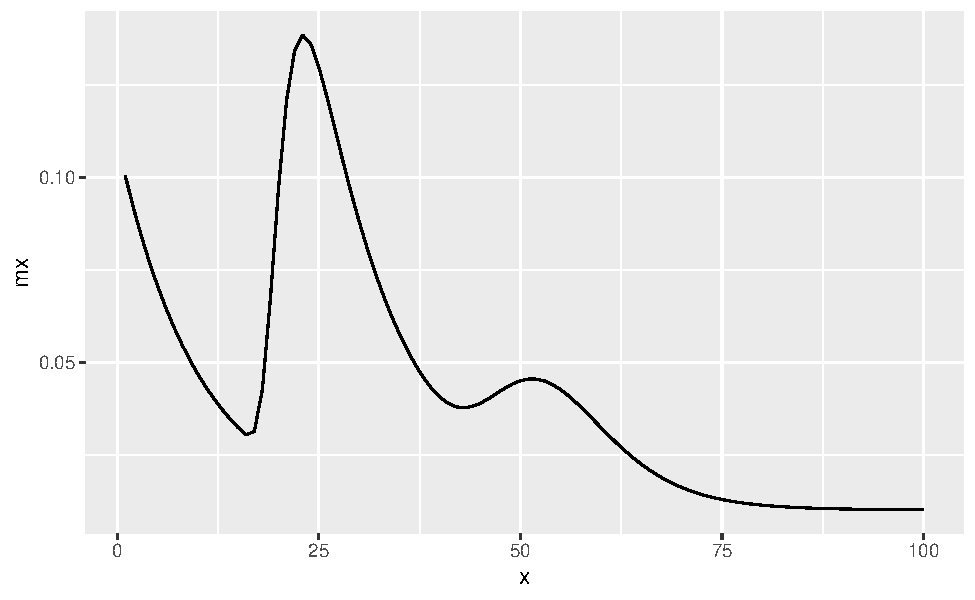
\includegraphics{_main_files/figure-latex/unnamed-chunk-80-1.pdf}

\hypertarget{model-schedules}{%
\section{Model schedules}\label{model-schedules}}

\hypertarget{model-migration-age-schedules}{%
\subsection{Model migration age schedules}\label{model-migration-age-schedules}}

\begin{itemize}
\tightlist
\item
  The \emph{migest} package contains two sets of parameters for model migration schedules.
\item
  The \texttt{rc\_model\_fund} are the set of fundamental parameters proposed by Rogers and Castro to represent a typical migration age pattern, based on their analysis of over 500 migration flows
\end{itemize}

\begin{Shaded}
\begin{Highlighting}[]
\FunctionTok{library}\NormalTok{(migest)}
\NormalTok{rc\_model\_fund}
\end{Highlighting}
\end{Shaded}

\begin{verbatim}
## # A tibble: 7 x 2
##   param    value
##   <chr>    <dbl>
## 1 a1       0.02 
## 2 alpha1   0.1  
## 3 a2       0.06 
## 4 alpha2   0.1  
## 5 mu2     20    
## 6 lambda2  0.4  
## 7 c        0.003
\end{verbatim}

\hypertarget{model-migration-age-schedules-1}{%
\subsection{Model migration age schedules}\label{model-migration-age-schedules-1}}

\begin{itemize}
\tightlist
\item
  Plot of model age schedule based on fundamental parameters
\end{itemize}

\begin{Shaded}
\begin{Highlighting}[]
\CommentTok{\# convert data frame to named vector}
\NormalTok{p }\OtherTok{\textless{}{-}} \FunctionTok{deframe}\NormalTok{(rc\_model\_fund)}
\NormalTok{p}
\end{Highlighting}
\end{Shaded}

\begin{verbatim}
##      a1  alpha1      a2  alpha2     mu2 lambda2       c 
##   2e-02   1e-01   6e-02   1e-01   2e+01   4e-01   3e-03
\end{verbatim}

\begin{Shaded}
\begin{Highlighting}[]
\FunctionTok{tibble}\NormalTok{(}\AttributeTok{x =} \DecValTok{1}\SpecialCharTok{:}\DecValTok{100}\NormalTok{, }
       \AttributeTok{mx =} \FunctionTok{mig\_calculate\_rc}\NormalTok{(}\AttributeTok{ages =}\NormalTok{ x, }\AttributeTok{pars =}\NormalTok{ p)) }\SpecialCharTok{\%\textgreater{}\%}
  \FunctionTok{ggplot}\NormalTok{(}\AttributeTok{mapping =} \FunctionTok{aes}\NormalTok{(}\AttributeTok{x =}\NormalTok{ x, }\AttributeTok{y =}\NormalTok{ mx)) }\SpecialCharTok{+}
  \FunctionTok{geom\_line}\NormalTok{()}
\end{Highlighting}
\end{Shaded}

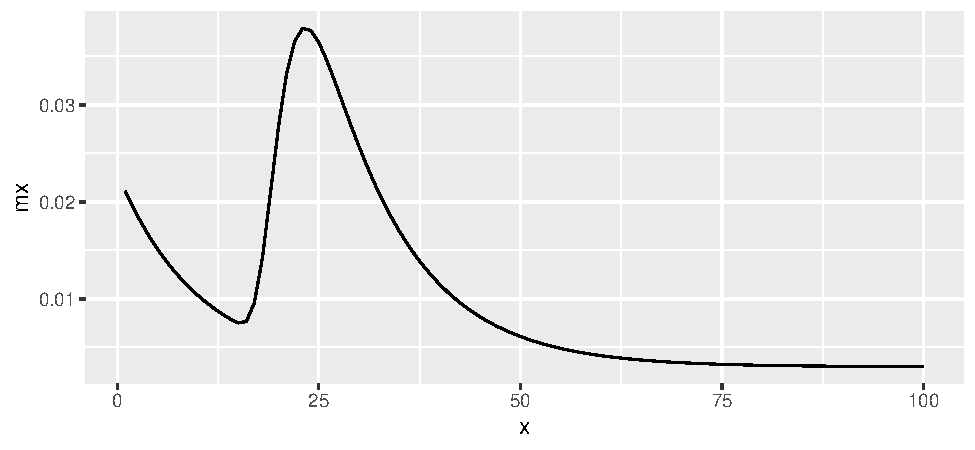
\includegraphics{_main_files/figure-latex/unnamed-chunk-82-1.pdf}

\hypertarget{model-migration-age-schedules-2}{%
\subsection{Model migration age schedules}\label{model-migration-age-schedules-2}}

\begin{itemize}
\tightlist
\item
  Rogers and Castro describe the nice properties in the parameters and their relationships
\item
  Peaking: early versus late peaking (\(\mu_2\))

  \begin{itemize}
  \tightlist
  \item
    \(\mu_2 = 20\) in the fundamental parameters
  \end{itemize}
\item
  Dominance: \(\gamma_{12} = a_1/a_2\) as the index of child dependency, and \(1/\gamma_{12}\) as index of labor dominance

  \begin{itemize}
  \tightlist
  \item
    \(\gamma_{12} = 1/3\) in fundamental parameters
  \end{itemize}
\item
  Labor asymmetry: \(\sigma_2 = \lambda_2/\alpha_2\)

  \begin{itemize}
  \tightlist
  \item
    \(\sigma_{2} = 4\) in fundamental parameters
  \end{itemize}
\item
  Regularity: \(\beta_{12} = \alpha_1/\alpha_2\) how the migration rates of children match to the migration rates of parents

  \begin{itemize}
  \tightlist
  \item
    \(\beta_{12} = 1\) in fundamental parameters
  \end{itemize}
\item
  Users can focus on these four measures (peaking, dominance, labor asymmetry and regularity) when describing or deriving their own model schedules
\end{itemize}

\hypertarget{model-migration-age-schedules-3}{%
\subsection{Model migration age schedules}\label{model-migration-age-schedules-3}}

\begin{itemize}
\tightlist
\item
  The \texttt{index\_age\_rc()} function in the migest package returns these ratios given a named vector of the parameters
\end{itemize}

\begin{Shaded}
\begin{Highlighting}[]
\NormalTok{rc\_model\_fund }\SpecialCharTok{\%\textgreater{}\%}
  \FunctionTok{deframe}\NormalTok{() }\SpecialCharTok{\%\textgreater{}\%}
  \FunctionTok{index\_age\_rc}\NormalTok{()}
\end{Highlighting}
\end{Shaded}

\begin{verbatim}
## # A tibble: 5 x 2
##   measure           value
##   <chr>             <dbl>
## 1 peaking          20    
## 2 child_dependency  0.333
## 3 labor_dependency  3    
## 4 labor_asymmetry   4    
## 5 regularity        1
\end{verbatim}

\hypertarget{model-migration-age-schedules-4}{%
\subsection{Model migration age schedules}\label{model-migration-age-schedules-4}}

\begin{itemize}
\tightlist
\item
  The \texttt{rc\_model\_un} are the set of fundamental parameters proposed in \citet{UnitedNations1992} for estimating age-specific migration flows in different contexts
\end{itemize}

\begin{Shaded}
\begin{Highlighting}[]
\NormalTok{rc\_model\_un}
\end{Highlighting}
\end{Shaded}

\begin{verbatim}
## # A tibble: 84 x 5
##    schedule         schedule_abb sex   param     value
##    <chr>            <chr>        <chr> <chr>     <dbl>
##  1 Western standard ws           male  a1       0.0215
##  2 Western standard ws           male  alpha1   0.105 
##  3 Western standard ws           male  a2       0.0694
##  4 Western standard ws           male  alpha2   0.112 
##  5 Western standard ws           male  mu2     20.0   
##  6 Western standard ws           male  lambda2  0.391 
##  7 Western standard ws           male  c        0.0028
##  8 Low dependency   ld           male  a1       0.0128
##  9 Low dependency   ld           male  alpha1   0.105 
## 10 Low dependency   ld           male  a2       0.0804
## # ... with 74 more rows
\end{verbatim}

\hypertarget{model-migration-age-schedules-5}{%
\subsection{Model migration age schedules}\label{model-migration-age-schedules-5}}

\begin{itemize}
\tightlist
\item
  To calculate model schedules we can use

  \begin{itemize}
  \tightlist
  \item
    \texttt{nest()} to group together the parameters
  \item
    \texttt{map()} to apply the parameters to the \texttt{mig\_calculate\_rc()} function for each group
  \end{itemize}
\end{itemize}

\begin{Shaded}
\begin{Highlighting}[]
\NormalTok{d }\OtherTok{\textless{}{-}}\NormalTok{ rc\_model\_un }\SpecialCharTok{\%\textgreater{}\%}
  \FunctionTok{select}\NormalTok{(}\SpecialCharTok{{-}}\NormalTok{schedule\_abb) }\SpecialCharTok{\%\textgreater{}\%}
  \FunctionTok{nest}\NormalTok{(}\AttributeTok{rc\_param =} \FunctionTok{c}\NormalTok{(param, value)) }\SpecialCharTok{\%\textgreater{}\%}
  \FunctionTok{mutate}\NormalTok{(}\AttributeTok{p =} \FunctionTok{map}\NormalTok{(}\AttributeTok{.x =}\NormalTok{ rc\_param, }\AttributeTok{.f =} \SpecialCharTok{\textasciitilde{}}\FunctionTok{deframe}\NormalTok{(.x)),}
         \AttributeTok{mx =} \FunctionTok{map}\NormalTok{(}\AttributeTok{.x =}\NormalTok{ p, }
                  \AttributeTok{.f =} \SpecialCharTok{\textasciitilde{}}\FunctionTok{mig\_calculate\_rc}\NormalTok{(}\AttributeTok{ages =} \DecValTok{1}\SpecialCharTok{:}\DecValTok{80}\NormalTok{, }\AttributeTok{pars =}\NormalTok{ .x)),}
         \AttributeTok{age =} \FunctionTok{list}\NormalTok{(}\DecValTok{1}\SpecialCharTok{:}\DecValTok{80}\NormalTok{))}
\NormalTok{d}
\end{Highlighting}
\end{Shaded}

\begin{verbatim}
## # A tibble: 12 x 6
##    schedule                              sex    rc_param    p      mx     age   
##    <chr>                                 <chr>  <list>      <list> <list> <list>
##  1 Western standard                      male   <tibble [7~ <dbl ~ <dbl ~ <int ~
##  2 Low dependency                        male   <tibble [7~ <dbl ~ <dbl ~ <int ~
##  3 High dependency                       male   <tibble [7~ <dbl ~ <dbl ~ <int ~
##  4 Young labour force entry              male   <tibble [7~ <dbl ~ <dbl ~ <int ~
##  5 Old labour force entry                male   <tibble [7~ <dbl ~ <dbl ~ <int ~
##  6 Low dependency low labour force entry male   <tibble [7~ <dbl ~ <dbl ~ <int ~
##  7 Western standard                      female <tibble [7~ <dbl ~ <dbl ~ <int ~
##  8 Low dependency                        female <tibble [7~ <dbl ~ <dbl ~ <int ~
##  9 High dependency                       female <tibble [7~ <dbl ~ <dbl ~ <int ~
## 10 Young labour force entry              female <tibble [7~ <dbl ~ <dbl ~ <int ~
## 11 Old labour force entry                female <tibble [7~ <dbl ~ <dbl ~ <int ~
## 12 Low dependency low labour force entry female <tibble [7~ <dbl ~ <dbl ~ <int ~
\end{verbatim}

\hypertarget{model-migration-age-schedules-6}{%
\subsection{Model migration age schedules}\label{model-migration-age-schedules-6}}

\begin{Shaded}
\begin{Highlighting}[]
\CommentTok{\# first row parameters}
\NormalTok{d}\SpecialCharTok{$}\NormalTok{p[[}\DecValTok{1}\NormalTok{]]}
\end{Highlighting}
\end{Shaded}

\begin{verbatim}
##      a1  alpha1      a2  alpha2     mu2 lambda2       c 
##  0.0215  0.1050  0.0694  0.1120 20.0400  0.3910  0.0028
\end{verbatim}

\begin{Shaded}
\begin{Highlighting}[]
\CommentTok{\# data unnested}
\NormalTok{d }\SpecialCharTok{\%\textgreater{}\%}
  \FunctionTok{select}\NormalTok{(}\SpecialCharTok{{-}}\NormalTok{rc\_param, }\SpecialCharTok{{-}}\NormalTok{p) }\SpecialCharTok{\%\textgreater{}\%}
  \FunctionTok{unnest}\NormalTok{(}\FunctionTok{c}\NormalTok{(mx, age))}
\end{Highlighting}
\end{Shaded}

\begin{verbatim}
## # A tibble: 960 x 4
##    schedule         sex       mx   age
##    <chr>            <chr>  <dbl> <int>
##  1 Western standard male  0.0222     1
##  2 Western standard male  0.0202     2
##  3 Western standard male  0.0185     3
##  4 Western standard male  0.0169     4
##  5 Western standard male  0.0155     5
##  6 Western standard male  0.0143     6
##  7 Western standard male  0.0131     7
##  8 Western standard male  0.0121     8
##  9 Western standard male  0.0112     9
## 10 Western standard male  0.0103    10
## # ... with 950 more rows
\end{verbatim}

\hypertarget{model-migration-age-schedules-7}{%
\subsection{Model migration age schedules}\label{model-migration-age-schedules-7}}

\begin{itemize}
\tightlist
\item
  Use \texttt{unnest()} to create a data base varying by age for each model schedule and sex for plotting
\end{itemize}

\begin{Shaded}
\begin{Highlighting}[]
\NormalTok{d }\SpecialCharTok{\%\textgreater{}\%}
  \FunctionTok{unnest}\NormalTok{(}\FunctionTok{c}\NormalTok{(mx, age)) }\SpecialCharTok{\%\textgreater{}\%}
  \FunctionTok{mutate}\NormalTok{(}\AttributeTok{schedule =} \FunctionTok{str\_wrap}\NormalTok{(schedule, }\AttributeTok{width =} \DecValTok{20}\NormalTok{)) }\SpecialCharTok{\%\textgreater{}\%}
  \FunctionTok{ggplot}\NormalTok{(}\AttributeTok{mapping =} \FunctionTok{aes}\NormalTok{(}\AttributeTok{x =}\NormalTok{ age, }\AttributeTok{y =}\NormalTok{ mx, }\AttributeTok{colour =}\NormalTok{ schedule)) }\SpecialCharTok{+}
  \FunctionTok{geom\_line}\NormalTok{() }\SpecialCharTok{+}
  \FunctionTok{facet\_wrap}\NormalTok{(}\AttributeTok{facets =} \StringTok{"sex"}\NormalTok{, }\AttributeTok{ncol =} \DecValTok{1}\NormalTok{)}
\end{Highlighting}
\end{Shaded}

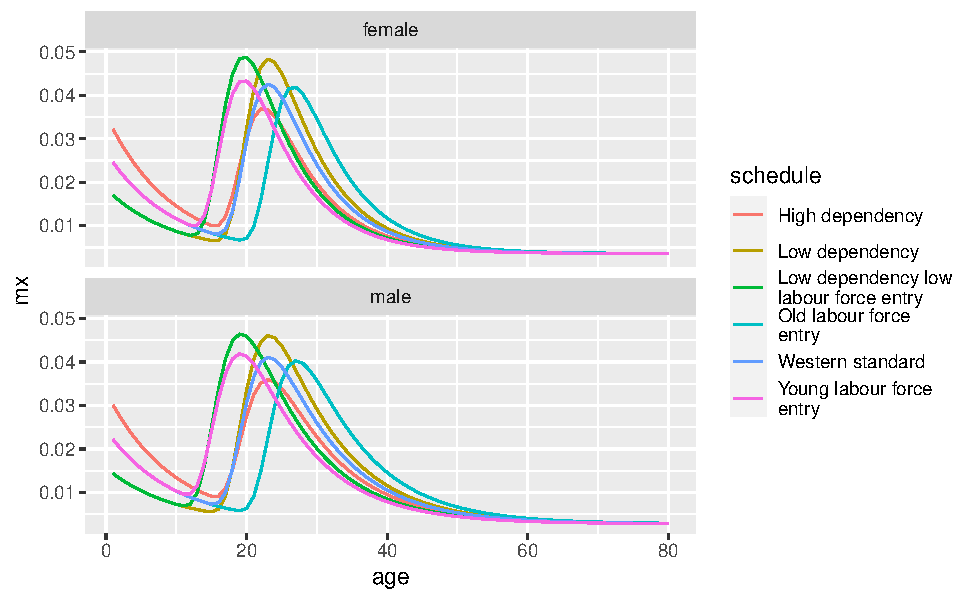
\includegraphics{_main_files/figure-latex/unnamed-chunk-87-1.pdf}

\hypertarget{model-migration-age-schedules-8}{%
\subsection{Model migration age schedules}\label{model-migration-age-schedules-8}}

\begin{itemize}
\tightlist
\item
  Model migration schedules are useful when we do not have any age information, but require an estimate of age specific migration

  \begin{itemize}
  \tightlist
  \item
    For example, in cohort component projections age specific migration rates are required but might not be available in any data source
  \end{itemize}
\item
  We may use an estimate or reported data on total migration to obtain age-specific migration

  \begin{itemize}
  \tightlist
  \item
    Design or select appropriate model age schedule based on existing knowledge of migration age patterns for the given flow.
  \end{itemize}
\end{itemize}

\begin{Shaded}
\begin{Highlighting}[]
\CommentTok{\# example for males based on young labour force entry}
\NormalTok{p }\OtherTok{\textless{}{-}}\NormalTok{ rc\_model\_un }\SpecialCharTok{\%\textgreater{}\%}
  \FunctionTok{filter}\NormalTok{(sex }\SpecialCharTok{==} \StringTok{"male"}\NormalTok{, schedule\_abb }\SpecialCharTok{==} \StringTok{"ylfe"}\NormalTok{) }\SpecialCharTok{\%\textgreater{}\%}
  \FunctionTok{select}\NormalTok{(param, value) }\SpecialCharTok{\%\textgreater{}\%}
  \FunctionTok{deframe}\NormalTok{()}
\NormalTok{p}
\end{Highlighting}
\end{Shaded}

\begin{verbatim}
##      a1  alpha1      a2  alpha2     mu2 lambda2       c 
##  0.0215  0.1050  0.0691  0.1120 16.0900  0.3910  0.0028
\end{verbatim}

\hypertarget{model-migration-age-schedules-9}{%
\subsection{Model migration age schedules}\label{model-migration-age-schedules-9}}

\begin{Shaded}
\begin{Highlighting}[]
\FunctionTok{tibble}\NormalTok{(}\AttributeTok{x =} \DecValTok{1}\SpecialCharTok{:}\DecValTok{90}\NormalTok{, }
       \AttributeTok{mx =} \FunctionTok{mig\_calculate\_rc}\NormalTok{(}\AttributeTok{ages =}\NormalTok{ x, }\AttributeTok{pars =}\NormalTok{ p),}
       \CommentTok{\# calculate number of migrants, given a total estimate of 10,000}
       \AttributeTok{Mx =} \DecValTok{10000} \SpecialCharTok{*}\NormalTok{ mx) }\SpecialCharTok{\%\textgreater{}\%}
  \FunctionTok{ggplot}\NormalTok{(}\AttributeTok{mapping =} \FunctionTok{aes}\NormalTok{(}\AttributeTok{x =}\NormalTok{ x, }\AttributeTok{y =}\NormalTok{ Mx)) }\SpecialCharTok{+}
  \FunctionTok{geom\_line}\NormalTok{()}
\end{Highlighting}
\end{Shaded}

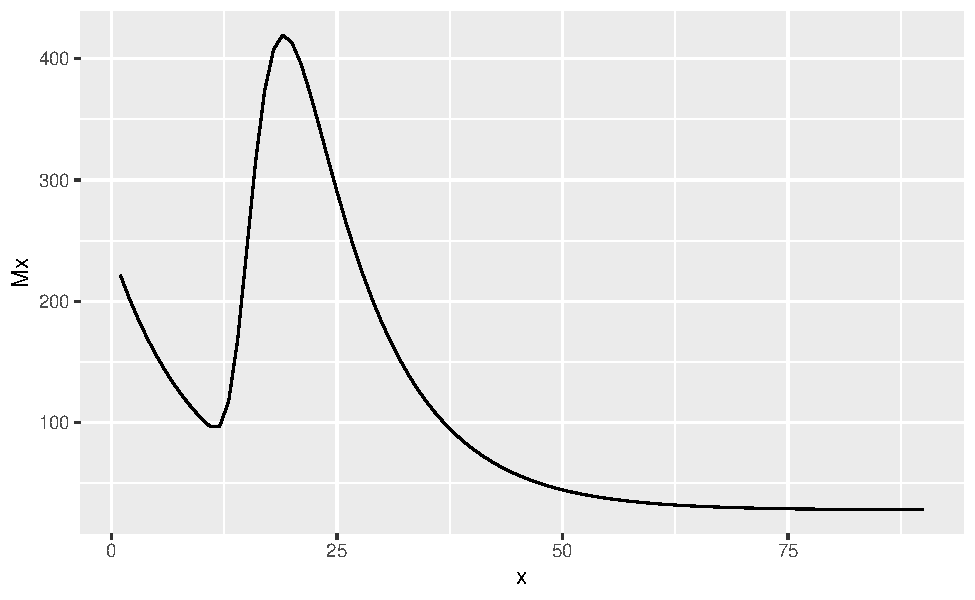
\includegraphics{_main_files/figure-latex/unnamed-chunk-89-1.pdf}

\hypertarget{fitting-schedules}{%
\section{Fitting schedules}\label{fitting-schedules}}

\hypertarget{fitting-roger-castro-migration-age-schedules}{%
\subsection{Fitting Roger Castro migration age schedules}\label{fitting-roger-castro-migration-age-schedules}}

\begin{itemize}
\tightlist
\item
  If we have age-specific migration data we might want to estimate the parameters of a Rogers Castro age schedule to

  \begin{itemize}
  \tightlist
  \item
    Smooth the data
  \item
    Analyse the parameter estimates
  \item
    Create projected age schedules based on past patterns of the age schedule parameters
  \end{itemize}
\item
  Fitting Rogers Castro migration age schedules can be difficult.

  \begin{itemize}
  \tightlist
  \item
    A number of different software has been used to fit age schedules including \citet{Rogers1994}, TableCurve 2D \citet{Rogers1999a}, MATLAB \citet{Rogers2010}, and Excel \citet{Wilson2010}.
  \end{itemize}
\item
  The \texttt{mig\_estimate\_rc()} function in DemoTools or rcbayes uses Stan, via the rstan package, a Bayesian probabilistic programming language

  \begin{itemize}
  \tightlist
  \item
    Estimation is carried out using MCMC sampling.
  \end{itemize}
\item
  Requires two arguments

  \begin{itemize}
  \tightlist
  \item
    \texttt{ages} a vector of migration ages
  \item
    \texttt{mx} a vector of standardized migration intensities for the corresponding ages
  \item
    Specify form of age schedule using the \texttt{pre\_working\_age}, \texttt{working\_age}, \texttt{retirement} and \texttt{post\_retirement} arguments - set to \texttt{TRUE} or \texttt{FALSE}
  \end{itemize}
\end{itemize}

\hypertarget{fitting-roger-castro-migration-age-schedules-1}{%
\subsection{Fitting Roger Castro migration age schedules}\label{fitting-roger-castro-migration-age-schedules-1}}

\begin{itemize}
\tightlist
\item
  Demonstrate with five-year data from the \texttt{italy\_area} data set in \emph{migest}

  \begin{itemize}
  \tightlist
  \item
    Calculate the out-migration for Islands (Sicily and Sardinia) in 1970
  \end{itemize}
\end{itemize}

\begin{Shaded}
\begin{Highlighting}[]
\CommentTok{\# include a numeric age column for mig\_estimate\_rc()}
\NormalTok{i }\OtherTok{\textless{}{-}}\NormalTok{ italy\_area }\SpecialCharTok{\%\textgreater{}\%}
  \FunctionTok{filter}\NormalTok{(year }\SpecialCharTok{==} \DecValTok{1970}\NormalTok{) }\SpecialCharTok{\%\textgreater{}\%}
  \FunctionTok{group\_by}\NormalTok{(age\_grp) }\SpecialCharTok{\%\textgreater{}\%}
  \FunctionTok{sum\_turnover}\NormalTok{() }\SpecialCharTok{\%\textgreater{}\%}
  \FunctionTok{filter}\NormalTok{(region }\SpecialCharTok{==} \StringTok{"Islands"}\NormalTok{) }\SpecialCharTok{\%\textgreater{}\%}
  \FunctionTok{separate}\NormalTok{(}\AttributeTok{col =}\NormalTok{ age\_grp, }\AttributeTok{into =} \FunctionTok{c}\NormalTok{(}\StringTok{"age\_min"}\NormalTok{, }\StringTok{"age\_max"}\NormalTok{), }
           \AttributeTok{remove =} \ConstantTok{FALSE}\NormalTok{, }\AttributeTok{convert =} \ConstantTok{TRUE}\NormalTok{)}
\end{Highlighting}
\end{Shaded}

\begin{verbatim}
## Adding missing grouping variables: `age_grp`
\end{verbatim}

\begin{Shaded}
\begin{Highlighting}[]
\NormalTok{i}
\end{Highlighting}
\end{Shaded}

\begin{verbatim}
## # A tibble: 20 x 8
## # Groups:   age_grp [20]
##    age_grp age_min age_max region  in_mig out_mig  turn   net
##    <fct>     <int>   <int> <chr>    <dbl>   <dbl> <dbl> <dbl>
##  1 0-4           0       4 Islands   4532    7876 12408 -3344
##  2 5-9           5       9 Islands   3592    7271 10863 -3679
##  3 10-14        10      14 Islands   2228    5779  8007 -3551
##  4 15-19        15      19 Islands   3064    8526 11590 -5462
##  5 20-24        20      24 Islands   6861   15629 22490 -8768
##  6 25-29        25      29 Islands   5891   11224 17115 -5333
##  7 30-34        30      34 Islands   4042    7046 11088 -3004
##  8 35-39        35      39 Islands   2480    4612  7092 -2132
##  9 40-44        40      44 Islands   1737    3634  5371 -1897
## 10 45-49        45      49 Islands   1383    2783  4166 -1400
## 11 50-54        50      54 Islands    910    1716  2626  -806
## 12 55-59        55      59 Islands    899    1587  2486  -688
## 13 60-64        60      64 Islands    789    1217  2006  -428
## 14 65-69        65      69 Islands    602     924  1526  -322
## 15 70-74        70      74 Islands    427     702  1129  -275
## 16 75-79        75      79 Islands    311     490   801  -179
## 17 80-84        80      84 Islands    158     268   426  -110
## 18 85-89        85      89 Islands     59     116   175   -57
## 19 90-94        90      94 Islands     17      35    52   -18
## 20 95+          95      NA Islands     95     137   232   -42
\end{verbatim}

\hypertarget{fitting-roger-castro-migration-age-schedules-2}{%
\subsection{Fitting Roger Castro migration age schedules}\label{fitting-roger-castro-migration-age-schedules-2}}

\begin{itemize}
\tightlist
\item
  Requires a standardized age schedule (where values sum to one)
\item
  Will take a few minutes and print out lots of messages from Stan
\end{itemize}

\begin{Shaded}
\begin{Highlighting}[]
\NormalTok{m }\OtherTok{\textless{}{-}}\NormalTok{ i}\SpecialCharTok{$}\NormalTok{out\_mig}\SpecialCharTok{/}\FunctionTok{sum}\NormalTok{(i}\SpecialCharTok{$}\NormalTok{out\_mig)}
\NormalTok{m}
\end{Highlighting}
\end{Shaded}

\begin{verbatim}
##  [1] 0.0965527387 0.0891359780 0.0708453881 0.1045211592 0.1915976070
##  [6] 0.1375962340 0.0863776786 0.0565390085 0.0445496004 0.0341170990
## [11] 0.0210366302 0.0194552052 0.0149193351 0.0113274163 0.0086058942
## [16] 0.0060069632 0.0032854411 0.0014220566 0.0004290688 0.0016794979
\end{verbatim}

\begin{Shaded}
\begin{Highlighting}[]
\NormalTok{f }\OtherTok{\textless{}{-}} \FunctionTok{mig\_estimate\_rc}\NormalTok{(}\AttributeTok{ages =}\NormalTok{ i}\SpecialCharTok{$}\NormalTok{age\_min }\SpecialCharTok{+} \FloatTok{2.5}\NormalTok{, }\AttributeTok{mx =}\NormalTok{ m,}
                     \CommentTok{\# set model components }
                     \AttributeTok{pre\_working\_age =} \ConstantTok{TRUE}\NormalTok{, }\AttributeTok{working\_age =} \ConstantTok{TRUE}\NormalTok{,}
                     \AttributeTok{retirement =} \ConstantTok{FALSE}\NormalTok{, }\AttributeTok{post\_retirement =} \ConstantTok{FALSE}\NormalTok{)}
\end{Highlighting}
\end{Shaded}

\begin{verbatim}
## 
## SAMPLING FOR MODEL 'f4d0f16f36ddb7179a67ef654e5d224a' NOW (CHAIN 1).
## Chain 1: 
## Chain 1: Gradient evaluation took 0 seconds
## Chain 1: 1000 transitions using 10 leapfrog steps per transition would take 0 seconds.
## Chain 1: Adjust your expectations accordingly!
## Chain 1: 
## Chain 1: 
## Chain 1: Iteration:    1 / 2000 [  0%]  (Warmup)
## Chain 1: Iteration:  200 / 2000 [ 10%]  (Warmup)
## Chain 1: Iteration:  400 / 2000 [ 20%]  (Warmup)
## Chain 1: Iteration:  600 / 2000 [ 30%]  (Warmup)
## Chain 1: Iteration:  800 / 2000 [ 40%]  (Warmup)
## Chain 1: Iteration: 1000 / 2000 [ 50%]  (Warmup)
## Chain 1: Iteration: 1001 / 2000 [ 50%]  (Sampling)
## Chain 1: Iteration: 1200 / 2000 [ 60%]  (Sampling)
## Chain 1: Iteration: 1400 / 2000 [ 70%]  (Sampling)
## Chain 1: Iteration: 1600 / 2000 [ 80%]  (Sampling)
## Chain 1: Iteration: 1800 / 2000 [ 90%]  (Sampling)
## Chain 1: Iteration: 2000 / 2000 [100%]  (Sampling)
## Chain 1: 
## Chain 1:  Elapsed Time: 0.695 seconds (Warm-up)
## Chain 1:                0.585 seconds (Sampling)
## Chain 1:                1.28 seconds (Total)
## Chain 1: 
## 
## SAMPLING FOR MODEL 'f4d0f16f36ddb7179a67ef654e5d224a' NOW (CHAIN 2).
## Chain 2: 
## Chain 2: Gradient evaluation took 0 seconds
## Chain 2: 1000 transitions using 10 leapfrog steps per transition would take 0 seconds.
## Chain 2: Adjust your expectations accordingly!
## Chain 2: 
## Chain 2: 
## Chain 2: Iteration:    1 / 2000 [  0%]  (Warmup)
## Chain 2: Iteration:  200 / 2000 [ 10%]  (Warmup)
## Chain 2: Iteration:  400 / 2000 [ 20%]  (Warmup)
## Chain 2: Iteration:  600 / 2000 [ 30%]  (Warmup)
## Chain 2: Iteration:  800 / 2000 [ 40%]  (Warmup)
## Chain 2: Iteration: 1000 / 2000 [ 50%]  (Warmup)
## Chain 2: Iteration: 1001 / 2000 [ 50%]  (Sampling)
## Chain 2: Iteration: 1200 / 2000 [ 60%]  (Sampling)
## Chain 2: Iteration: 1400 / 2000 [ 70%]  (Sampling)
## Chain 2: Iteration: 1600 / 2000 [ 80%]  (Sampling)
## Chain 2: Iteration: 1800 / 2000 [ 90%]  (Sampling)
## Chain 2: Iteration: 2000 / 2000 [100%]  (Sampling)
## Chain 2: 
## Chain 2:  Elapsed Time: 0.754 seconds (Warm-up)
## Chain 2:                0.617 seconds (Sampling)
## Chain 2:                1.371 seconds (Total)
## Chain 2: 
## 
## SAMPLING FOR MODEL 'f4d0f16f36ddb7179a67ef654e5d224a' NOW (CHAIN 3).
## Chain 3: 
## Chain 3: Gradient evaluation took 0 seconds
## Chain 3: 1000 transitions using 10 leapfrog steps per transition would take 0 seconds.
## Chain 3: Adjust your expectations accordingly!
## Chain 3: 
## Chain 3: 
## Chain 3: Iteration:    1 / 2000 [  0%]  (Warmup)
## Chain 3: Iteration:  200 / 2000 [ 10%]  (Warmup)
## Chain 3: Iteration:  400 / 2000 [ 20%]  (Warmup)
## Chain 3: Iteration:  600 / 2000 [ 30%]  (Warmup)
## Chain 3: Iteration:  800 / 2000 [ 40%]  (Warmup)
## Chain 3: Iteration: 1000 / 2000 [ 50%]  (Warmup)
## Chain 3: Iteration: 1001 / 2000 [ 50%]  (Sampling)
## Chain 3: Iteration: 1200 / 2000 [ 60%]  (Sampling)
## Chain 3: Iteration: 1400 / 2000 [ 70%]  (Sampling)
## Chain 3: Iteration: 1600 / 2000 [ 80%]  (Sampling)
## Chain 3: Iteration: 1800 / 2000 [ 90%]  (Sampling)
## Chain 3: Iteration: 2000 / 2000 [100%]  (Sampling)
## Chain 3: 
## Chain 3:  Elapsed Time: 0.771 seconds (Warm-up)
## Chain 3:                0.67 seconds (Sampling)
## Chain 3:                1.441 seconds (Total)
## Chain 3: 
## 
## SAMPLING FOR MODEL 'f4d0f16f36ddb7179a67ef654e5d224a' NOW (CHAIN 4).
## Chain 4: 
## Chain 4: Gradient evaluation took 0 seconds
## Chain 4: 1000 transitions using 10 leapfrog steps per transition would take 0 seconds.
## Chain 4: Adjust your expectations accordingly!
## Chain 4: 
## Chain 4: 
## Chain 4: Iteration:    1 / 2000 [  0%]  (Warmup)
## Chain 4: Iteration:  200 / 2000 [ 10%]  (Warmup)
## Chain 4: Iteration:  400 / 2000 [ 20%]  (Warmup)
## Chain 4: Iteration:  600 / 2000 [ 30%]  (Warmup)
## Chain 4: Iteration:  800 / 2000 [ 40%]  (Warmup)
## Chain 4: Iteration: 1000 / 2000 [ 50%]  (Warmup)
## Chain 4: Iteration: 1001 / 2000 [ 50%]  (Sampling)
## Chain 4: Iteration: 1200 / 2000 [ 60%]  (Sampling)
## Chain 4: Iteration: 1400 / 2000 [ 70%]  (Sampling)
## Chain 4: Iteration: 1600 / 2000 [ 80%]  (Sampling)
## Chain 4: Iteration: 1800 / 2000 [ 90%]  (Sampling)
## Chain 4: Iteration: 2000 / 2000 [100%]  (Sampling)
## Chain 4: 
## Chain 4:  Elapsed Time: 0.716 seconds (Warm-up)
## Chain 4:                0.684 seconds (Sampling)
## Chain 4:                1.4 seconds (Total)
## Chain 4:
\end{verbatim}

\hypertarget{fitting-roger-castro-migration-age-schedules-3}{%
\subsection{Fitting Roger Castro migration age schedules}\label{fitting-roger-castro-migration-age-schedules-3}}

The fitted object has two components

\begin{Shaded}
\begin{Highlighting}[]
\CommentTok{\# parameter estimates}
\NormalTok{f[[}\DecValTok{1}\NormalTok{]]}
\end{Highlighting}
\end{Shaded}

\begin{verbatim}
## # A tibble: 7 x 4
##   variable     median      lower    upper
##   <chr>         <dbl>      <dbl>    <dbl>
## 1 a1[1]       0.107    0.0943     0.118  
## 2 a2[1]       0.341    0.275      0.381  
## 3 alpha1[1]   0.0322   0.0270     0.0416 
## 4 alpha2[1]   0.227    0.152      0.301  
## 5 c           0.00157  0.0000724  0.00752
## 6 lambda2[1]  0.185    0.151      0.285  
## 7 mu2[1]     24.6     20.8       27.0
\end{verbatim}

\begin{Shaded}
\begin{Highlighting}[]
\CommentTok{\# fitted schedule}
\NormalTok{f[[}\DecValTok{2}\NormalTok{]]}
\end{Highlighting}
\end{Shaded}

\begin{verbatim}
## # A tibble: 20 x 6
##      age     data  median   lower  upper     diff_sq
##    <dbl>    <dbl>   <dbl>   <dbl>  <dbl>       <dbl>
##  1   2.5 0.0966   0.100   0.0902  0.111  0.0000152  
##  2   7.5 0.0891   0.0857  0.0775  0.0937 0.0000121  
##  3  12.5 0.0708   0.0738  0.0673  0.0804 0.00000881 
##  4  17.5 0.105    0.107   0.0935  0.120  0.00000573 
##  5  22.5 0.192    0.183   0.168   0.196  0.0000682  
##  6  27.5 0.138    0.144   0.133   0.154  0.0000459  
##  7  32.5 0.0864   0.0842  0.0725  0.0945 0.00000456 
##  8  37.5 0.0565   0.0506  0.0433  0.0587 0.0000357  
##  9  42.5 0.0445   0.0350  0.0299  0.0403 0.0000904  
## 10  47.5 0.0341   0.0272  0.0226  0.0316 0.0000483  
## 11  52.5 0.0210   0.0223  0.0178  0.0271 0.00000172 
## 12  57.5 0.0195   0.0190  0.0145  0.0237 0.000000235
## 13  62.5 0.0149   0.0163  0.0122  0.0210 0.00000203 
## 14  67.5 0.0113   0.0142  0.0102  0.0186 0.00000806 
## 15  72.5 0.00861  0.0124  0.00868 0.0167 0.0000141  
## 16  77.5 0.00601  0.0108  0.00734 0.0149 0.0000231  
## 17  82.5 0.00329  0.00949 0.00628 0.0136 0.0000385  
## 18  87.5 0.00142  0.00837 0.00537 0.0125 0.0000483  
## 19  92.5 0.000429 0.00738 0.00462 0.0115 0.0000483  
## 20  97.5 0.00168  0.00655 0.00398 0.0107 0.0000238
\end{verbatim}

\hypertarget{fitting-roger-castro-migration-age-schedules-4}{%
\subsection{Fitting Roger Castro migration age schedules}\label{fitting-roger-castro-migration-age-schedules-4}}

\begin{Shaded}
\begin{Highlighting}[]
\FunctionTok{ggplot}\NormalTok{(}\AttributeTok{data =}\NormalTok{ f[[}\DecValTok{2}\NormalTok{]], }
       \AttributeTok{mapping =} \FunctionTok{aes}\NormalTok{(}\AttributeTok{x =}\NormalTok{ age, }\AttributeTok{y =}\NormalTok{ data)) }\SpecialCharTok{+}
  \FunctionTok{geom\_ribbon}\NormalTok{(}\AttributeTok{mapping =} \FunctionTok{aes}\NormalTok{(}\AttributeTok{ymin =}\NormalTok{ lower, }\AttributeTok{ymax =}\NormalTok{ upper), }\AttributeTok{fill =} \StringTok{"lightblue"}\NormalTok{) }\SpecialCharTok{+}
  \FunctionTok{geom\_line}\NormalTok{(}\AttributeTok{mapping =} \FunctionTok{aes}\NormalTok{(}\AttributeTok{y =}\NormalTok{ median), }\AttributeTok{colour =} \StringTok{"blue"}\NormalTok{) }\SpecialCharTok{+}
  \FunctionTok{geom\_point}\NormalTok{() }
\end{Highlighting}
\end{Shaded}

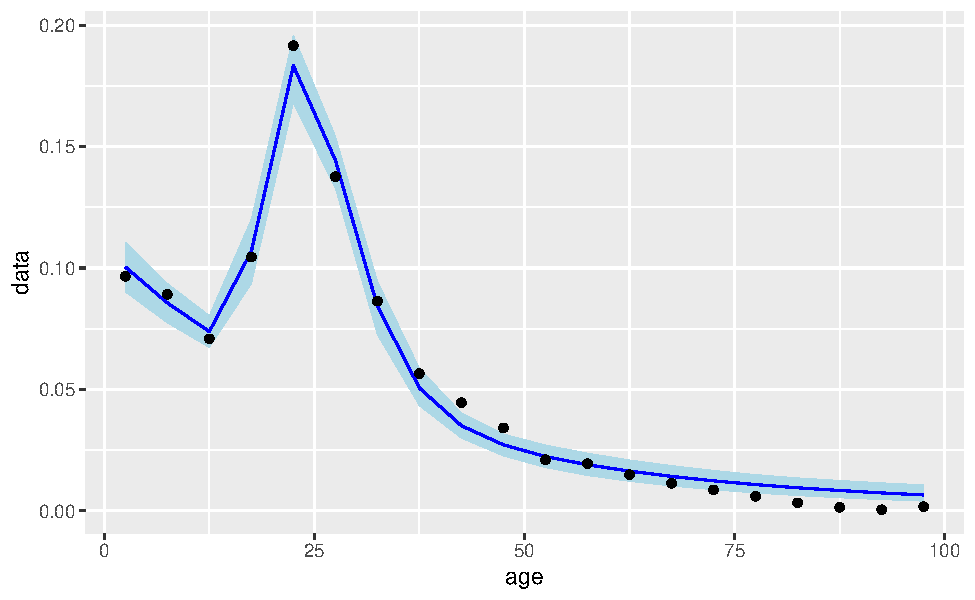
\includegraphics{_main_files/figure-latex/unnamed-chunk-93-1.pdf}

\hypertarget{fitting-roger-castro-migration-age-schedules-5}{%
\subsection{Fitting Roger Castro migration age schedules}\label{fitting-roger-castro-migration-age-schedules-5}}

\begin{itemize}
\tightlist
\item
  The \emph{migraR} package by Ruiz-Santacruz and Garcés also has functions to estimate parameters in Rogers Castro schedule

  \begin{itemize}
  \tightlist
  \item
    Also not on CRAN
  \item
    Uses an optimization procedure (non-Bayesian)
  \item
    Functions to select best form schedule
  \end{itemize}
\item
  Selecting the form of the schedule usually requires some form of visual inspection
\end{itemize}

\hypertarget{age-indices}{%
\section{Age Indices}\label{age-indices}}

\hypertarget{age-indices-1}{%
\subsection{Age Indices}\label{age-indices-1}}

\begin{itemize}
\tightlist
\item
  Number of criticisms of model age schedules for migration (\citet{Bell2002}, \citet{Bernard2014})
\item
  Not always clear how many parameters should be included in model schedule

  \begin{itemize}
  \tightlist
  \item
    Parameter estimates sensitive to the choice of model form, making comparisons difficult
  \item
    Use statistical accuracy measures to select best form, at the risk of over fitting
  \end{itemize}
\item
  Parameter estimates sensitive to initial values

  \begin{itemize}
  \tightlist
  \item
    Unlikely to be the case when using \texttt{mig\_estimate\_rc()}
  \end{itemize}
\item
  Unstable parameter estimates

  \begin{itemize}
  \tightlist
  \item
    Sensitive to measurement error in age-specific migration
  \end{itemize}
\item
  Interpretation of parameter estimates

  \begin{itemize}
  \tightlist
  \item
    The indexes in \texttt{index\_age\_rc()} have not been widely adopted, probably because of difficulty in fitting model schedules.
  \end{itemize}
\end{itemize}

\hypertarget{age-indices-2}{%
\subsection{Age Indices}\label{age-indices-2}}

\begin{itemize}
\tightlist
\item
  A number of other measures of age specific migration have been proposed that do not require fitting model age schedules.
\item
  Most a dependent on the migration intensity \(m_{as}\), the number of migrants in a age group and given time period as a percentage of the population at risk of moving.
\item
  \citet{Rogers1975} proposed a Gross Migraproduction Rate (GMR) based on the sum of age-specific (and sex-specific) migration intensities
  \[
  GMR = \sum_{as} m_{as}
  \]
\item
  \citet{Bell2002} introduced

  \begin{itemize}
  \tightlist
  \item
    Peak migration intensity, the largest age-specific migration intensity of any age-group
  \item
    Peak age, the corresponding age of the peak migration intensity
  \end{itemize}
\end{itemize}

\hypertarget{age-indices-3}{%
\subsection{Age Indices}\label{age-indices-3}}

\begin{itemize}
\tightlist
\item
  \citet{Bell2009} proposed and additional measures

  \begin{itemize}
  \tightlist
  \item
    Breadth of peak based on the sum of the peak migration intensity at the peak age and the five age-groups before and after the peak.
  \item
    Peak share based on the percentage of the normalized migration age schedule covered by the peak age and the five age-groups before and after the peak.
  \end{itemize}
\item
  \citet{Bernard2014} provide three additioanl measures

  \begin{itemize}
  \tightlist
  \item
    The Maximum Upward Rate of Change (MURC) for the largest gradient in the slope of the labour force peak before the peak age
  \item
    The Maximum Downward Rate of Change (MDRC) for the largest gradient in the slope of the labour force peak after the peak age
  \item
    The asymmetry of the labour force peak based on the ratio of MURC and MDRC
  \end{itemize}
\item
  Each of these measures area calculated in the \texttt{age\_index()} function in the \emph{migest} package
\end{itemize}

\hypertarget{age-indices-4}{%
\subsection{Age Indices}\label{age-indices-4}}

\begin{itemize}
\tightlist
\item
  To demonstrate we use the age schedule data of Brazil 2000 and France 2006 in the \texttt{ipumsi\_age} data frame of the \emph{migest} package

  \begin{itemize}
  \tightlist
  \item
    Migration based on five-year transitions between any minor (and major) administrative units.
  \end{itemize}
\end{itemize}

\begin{Shaded}
\begin{Highlighting}[]
\NormalTok{ipumsi\_age }\SpecialCharTok{\%\textgreater{}\%}
  \FunctionTok{mutate}\NormalTok{(}\AttributeTok{mi =}\NormalTok{ migrants}\SpecialCharTok{/}\NormalTok{population) }\SpecialCharTok{\%\textgreater{}\%}
  \FunctionTok{filter}\NormalTok{(age }\SpecialCharTok{\textgreater{}} \DecValTok{5}\NormalTok{) }\SpecialCharTok{\%\textgreater{}\%}
  \FunctionTok{ggplot}\NormalTok{(}\AttributeTok{mapping =} \FunctionTok{aes}\NormalTok{(}\AttributeTok{x =}\NormalTok{ age, }\AttributeTok{y =}\NormalTok{ mi)) }\SpecialCharTok{+}
  \FunctionTok{geom\_line}\NormalTok{() }\SpecialCharTok{+}
  \FunctionTok{facet\_wrap}\NormalTok{(}\AttributeTok{facets =} \StringTok{"sample"}\NormalTok{, }\AttributeTok{scales =} \StringTok{"free"}\NormalTok{)}
\end{Highlighting}
\end{Shaded}

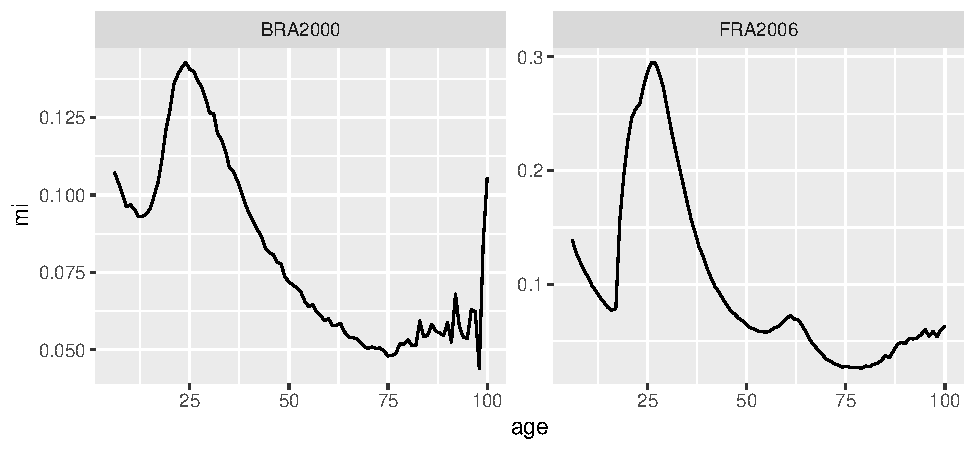
\includegraphics{_main_files/figure-latex/unnamed-chunk-94-1.pdf}

\hypertarget{age-indices-5}{%
\subsection{Age Indices}\label{age-indices-5}}

\begin{itemize}
\tightlist
\item
  \citet{Bernard2014} recommends smoothing age schedules before calculating index values

  \begin{itemize}
  \tightlist
  \item
    Get very similar results without smoothing - at least in these examples
  \end{itemize}
\item
  \texttt{index\_age()} by default ignores values above 65 (and below 5) when calculating peak index statistics\\

  \begin{itemize}
  \tightlist
  \item
    GMR still sensitive for outliers (e.g.~oldest in Brazil)
  \end{itemize}
\item
  Index values for Brazil 2000
\end{itemize}

\begin{Shaded}
\begin{Highlighting}[]
\NormalTok{ipumsi\_age }\SpecialCharTok{\%\textgreater{}\%}
  \FunctionTok{filter}\NormalTok{(sample }\SpecialCharTok{==} \StringTok{"BRA2000"}\NormalTok{) }\SpecialCharTok{\%\textgreater{}\%}
  \FunctionTok{mutate}\NormalTok{(}\AttributeTok{mi =}\NormalTok{ migrants}\SpecialCharTok{/}\NormalTok{population) }\SpecialCharTok{\%\textgreater{}\%}
  \FunctionTok{index\_age}\NormalTok{()}
\end{Highlighting}
\end{Shaded}

\begin{verbatim}
## # A tibble: 8 x 2
##   measure        value
##   <chr>          <dbl>
## 1 gmr            7.82 
## 2 peak_mi       14.3  
## 3 peak_age      24    
## 4 peak_breadth 147.   
## 5 peak_share    18.8  
## 6 murc          19    
## 7 mdrc          32    
## 8 asymmetry      0.594
\end{verbatim}

\hypertarget{age-indices-6}{%
\subsection{Age Indices}\label{age-indices-6}}

\begin{itemize}
\tightlist
\item
  Index values are most useful for comparing age-specific migration in different countries (or regions or time periods)
\end{itemize}

\begin{Shaded}
\begin{Highlighting}[]
\NormalTok{ipumsi\_age }\SpecialCharTok{\%\textgreater{}\%}
  \FunctionTok{group\_by}\NormalTok{(sample) }\SpecialCharTok{\%\textgreater{}\%}
  \FunctionTok{mutate}\NormalTok{(}\AttributeTok{mi =}\NormalTok{ migrants}\SpecialCharTok{/}\NormalTok{population) }\SpecialCharTok{\%\textgreater{}\%}
  \FunctionTok{index\_age}\NormalTok{() }\SpecialCharTok{\%\textgreater{}\%}
  \FunctionTok{pivot\_wider}\NormalTok{(}\AttributeTok{names\_from =}\NormalTok{ sample, }\AttributeTok{values\_from =}\NormalTok{ value)}
\end{Highlighting}
\end{Shaded}

\begin{verbatim}
## # A tibble: 8 x 3
##   measure      BRA2000 FRA2006
##   <chr>          <dbl>   <dbl>
## 1 gmr            7.82     9.55
## 2 peak_mi       14.3     29.5 
## 3 peak_age      24       26   
## 4 peak_breadth 147.     295.  
## 5 peak_share    18.8     30.8 
## 6 murc          19       18   
## 7 mdrc          32       30   
## 8 asymmetry      0.594    0.6
\end{verbatim}

\hypertarget{smoothing}{%
\section{Smoothing}\label{smoothing}}

\hypertarget{general-purpose-smoothing-functions}{%
\subsection{General purpose smoothing functions}\label{general-purpose-smoothing-functions}}

\begin{itemize}
\tightlist
\item
  There are many non-parametric smoothing functions in R that can be used to smooth data.
\item
  The \texttt{stats} package, which is loaded when R opens, includes

  \begin{itemize}
  \tightlist
  \item
    \texttt{ksmooth()} is a kernel regression smoother
  \item
    \texttt{loess.smooth()} is a Local Polynomial Regression Fitting method
  \item
    \texttt{smooth.spline} a cubic spline fit
  \end{itemize}
\item
  The DemoTools package contains a \texttt{smooth\_age\_5()} that is particularly useful for age-heaped data.
\end{itemize}

\hypertarget{general-purpose-smoothing-functions-1}{%
\subsection{General purpose smoothing functions}\label{general-purpose-smoothing-functions-1}}

\begin{itemize}
\tightlist
\item
  Smoothing methods perform some form of weighting data points on separate subsections (windows or bandwidths of the data)
\item
  In a migration age schedule context, this involves some form of simple local regression or averaging of migration intensities at each age, given data from nearby ages.
\item
  Careful consideration is usually required in choosing the bandwidth.

  \begin{itemize}
  \tightlist
  \item
    The default values are not always sensible for migration age schedules
  \end{itemize}
\item
  Might consider censoring the very oldest values where values can become volatile due to small numbers
\end{itemize}

\hypertarget{general-purpose-smoothing-functions-2}{%
\subsection{General purpose smoothing functions}\label{general-purpose-smoothing-functions-2}}

\begin{itemize}
\tightlist
\item
  Use Brazil 2000 IPUMS International sample data to demonstrate

  \begin{itemize}
  \tightlist
  \item
    Particularly rough at older age groups
  \end{itemize}
\end{itemize}

\begin{Shaded}
\begin{Highlighting}[]
\NormalTok{b }\OtherTok{\textless{}{-}}\NormalTok{ ipumsi\_age }\SpecialCharTok{\%\textgreater{}\%}
  \FunctionTok{filter}\NormalTok{(sample }\SpecialCharTok{==} \StringTok{"BRA2000"}\NormalTok{,}
\NormalTok{         age }\SpecialCharTok{\textgreater{}} \DecValTok{5}\NormalTok{) }\SpecialCharTok{\%\textgreater{}\%}
  \FunctionTok{mutate}\NormalTok{(}\AttributeTok{mi =}\NormalTok{ migrants}\SpecialCharTok{/}\NormalTok{population)  }

\FunctionTok{ggplot}\NormalTok{(}\AttributeTok{data =}\NormalTok{ b, }\AttributeTok{mapping =} \FunctionTok{aes}\NormalTok{(}\AttributeTok{x =}\NormalTok{ age, }\AttributeTok{y =}\NormalTok{ mi)) }\SpecialCharTok{+}
  \FunctionTok{geom\_point}\NormalTok{() }
\end{Highlighting}
\end{Shaded}

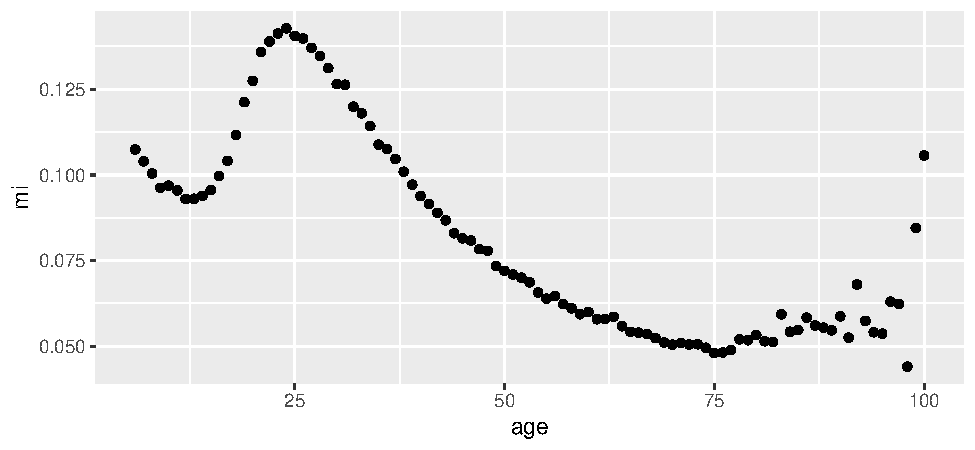
\includegraphics{_main_files/figure-latex/unnamed-chunk-97-1.pdf}

\hypertarget{general-purpose-smoothing-functions-3}{%
\subsection{General purpose smoothing functions}\label{general-purpose-smoothing-functions-3}}

\begin{itemize}
\tightlist
\item
  Most smoothing function in R require two vectors (\texttt{x} and \texttt{y})

  \begin{itemize}
  \tightlist
  \item
    Optional arguments to control the smoothness of the fit( names differ for different smoothing functions)
  \end{itemize}
\item
  Will return a list with two components (\texttt{x} and \texttt{y}), where the length of x may differ from the original vector provided

  \begin{itemize}
  \tightlist
  \item
    Set a output length argument (names differ for different smoothing functions)
  \item
    The \texttt{x} component will match age values
  \item
    Can use within \texttt{mutate()}
  \end{itemize}
\end{itemize}

\begin{Shaded}
\begin{Highlighting}[]
\NormalTok{k1 }\OtherTok{\textless{}{-}} \FunctionTok{ksmooth}\NormalTok{(}\AttributeTok{x =}\NormalTok{ b}\SpecialCharTok{$}\NormalTok{age, }\AttributeTok{y =}\NormalTok{ b}\SpecialCharTok{$}\NormalTok{mi)}
\FunctionTok{str}\NormalTok{(k1)}
\end{Highlighting}
\end{Shaded}

\begin{verbatim}
## List of 2
##  $ x: num [1:100] 6 6.95 7.9 8.85 9.8 ...
##  $ y: num [1:100] 0.1074 0.104 0.1004 0.0962 0.0969 ...
\end{verbatim}

\begin{Shaded}
\begin{Highlighting}[]
\NormalTok{k2 }\OtherTok{\textless{}{-}} \FunctionTok{ksmooth}\NormalTok{(}\AttributeTok{x =}\NormalTok{ b}\SpecialCharTok{$}\NormalTok{age, }\AttributeTok{y =}\NormalTok{ b}\SpecialCharTok{$}\NormalTok{mi, }\AttributeTok{n.points =} \FunctionTok{nrow}\NormalTok{(b))}
\FunctionTok{str}\NormalTok{(k2)}
\end{Highlighting}
\end{Shaded}

\begin{verbatim}
## List of 2
##  $ x: num [1:95] 6 7 8 9 10 11 12 13 14 15 ...
##  $ y: num [1:95] 0.1074 0.104 0.1004 0.0962 0.0969 ...
\end{verbatim}

\hypertarget{kernal-smoothing}{%
\subsection{Kernal smoothing}\label{kernal-smoothing}}

\begin{itemize}
\tightlist
\item
  The \texttt{ksmooth} function is unlikely to smooth a migration age schedule as the default bandwidth parameter is too small

  \begin{itemize}
  \tightlist
  \item
    Increase for a more suitable fit
  \end{itemize}
\end{itemize}

\begin{Shaded}
\begin{Highlighting}[]
\NormalTok{b }\OtherTok{\textless{}{-}}\NormalTok{ b }\SpecialCharTok{\%\textgreater{}\%} 
  \FunctionTok{mutate}\NormalTok{(}
    \AttributeTok{k\_default =} \FunctionTok{ksmooth}\NormalTok{(}\AttributeTok{x =}\NormalTok{ age, }\AttributeTok{y =}\NormalTok{ mi, }\AttributeTok{n.points =} \FunctionTok{n}\NormalTok{())}\SpecialCharTok{$}\NormalTok{y,}
    \AttributeTok{k\_bw5 =} \FunctionTok{ksmooth}\NormalTok{(}\AttributeTok{x =}\NormalTok{ age, }\AttributeTok{y =}\NormalTok{ mi, }\AttributeTok{n.points =} \FunctionTok{n}\NormalTok{(), }\AttributeTok{bandwidth =} \DecValTok{5}\NormalTok{)}\SpecialCharTok{$}\NormalTok{y,}
    \AttributeTok{k\_bw10 =} \FunctionTok{ksmooth}\NormalTok{(}\AttributeTok{x =}\NormalTok{ age, }\AttributeTok{y =}\NormalTok{ mi, }\AttributeTok{n.points =} \FunctionTok{n}\NormalTok{(), }\AttributeTok{bandwidth =} \DecValTok{10}\NormalTok{)}\SpecialCharTok{$}\NormalTok{y}
\NormalTok{  )}
\NormalTok{b}
\end{Highlighting}
\end{Shaded}

\begin{verbatim}
## # A tibble: 95 x 8
##    sample    age migrants population     mi k_default  k_bw5 k_bw10
##    <chr>   <dbl>    <dbl>      <dbl>  <dbl>     <dbl>  <dbl>  <dbl>
##  1 BRA2000     6  355723.   3311728. 0.107     0.107  0.104  0.100 
##  2 BRA2000     7  343852.   3307567. 0.104     0.104  0.102  0.0990
##  3 BRA2000     8  327166.   3258046. 0.100     0.100  0.101  0.0983
##  4 BRA2000     9  314905.   3272305. 0.0962    0.0962 0.0986 0.0978
##  5 BRA2000    10  324066.   3345583. 0.0969    0.0969 0.0964 0.0976
##  6 BRA2000    11  329525.   3451739. 0.0955    0.0955 0.0949 0.0978
##  7 BRA2000    12  327113.   3518160. 0.0930    0.0930 0.0944 0.0975
##  8 BRA2000    13  323180.   3473133. 0.0931    0.0931 0.0942 0.0982
##  9 BRA2000    14  334783.   3566239. 0.0939    0.0939 0.0950 0.100 
## 10 BRA2000    15  337297.   3528845. 0.0956    0.0956 0.0973 0.103 
## # ... with 85 more rows
\end{verbatim}

\hypertarget{kernal-smoothing-1}{%
\subsection{Kernal smoothing}\label{kernal-smoothing-1}}

\begin{Shaded}
\begin{Highlighting}[]
\FunctionTok{ggplot}\NormalTok{(}\AttributeTok{data =}\NormalTok{ b, }\AttributeTok{mapping =} \FunctionTok{aes}\NormalTok{(}\AttributeTok{x =}\NormalTok{ age, }\AttributeTok{y =}\NormalTok{ mi)) }\SpecialCharTok{+}
  \FunctionTok{geom\_point}\NormalTok{(}\AttributeTok{alpha =} \FloatTok{0.5}\NormalTok{) }\SpecialCharTok{+} 
  \FunctionTok{geom\_line}\NormalTok{(}\AttributeTok{mapping =} \FunctionTok{aes}\NormalTok{(}\AttributeTok{y =}\NormalTok{ k\_default), }\AttributeTok{col =} \StringTok{"darkgrey"}\NormalTok{) }\SpecialCharTok{+}
  \FunctionTok{geom\_line}\NormalTok{(}\AttributeTok{mapping =} \FunctionTok{aes}\NormalTok{(}\AttributeTok{y =}\NormalTok{ k\_bw5), }\AttributeTok{col =} \StringTok{"orange"}\NormalTok{) }\SpecialCharTok{+}
  \FunctionTok{geom\_line}\NormalTok{(}\AttributeTok{mapping =} \FunctionTok{aes}\NormalTok{(}\AttributeTok{y =}\NormalTok{ k\_bw10), }\AttributeTok{col =} \StringTok{"red"}\NormalTok{)}
\end{Highlighting}
\end{Shaded}

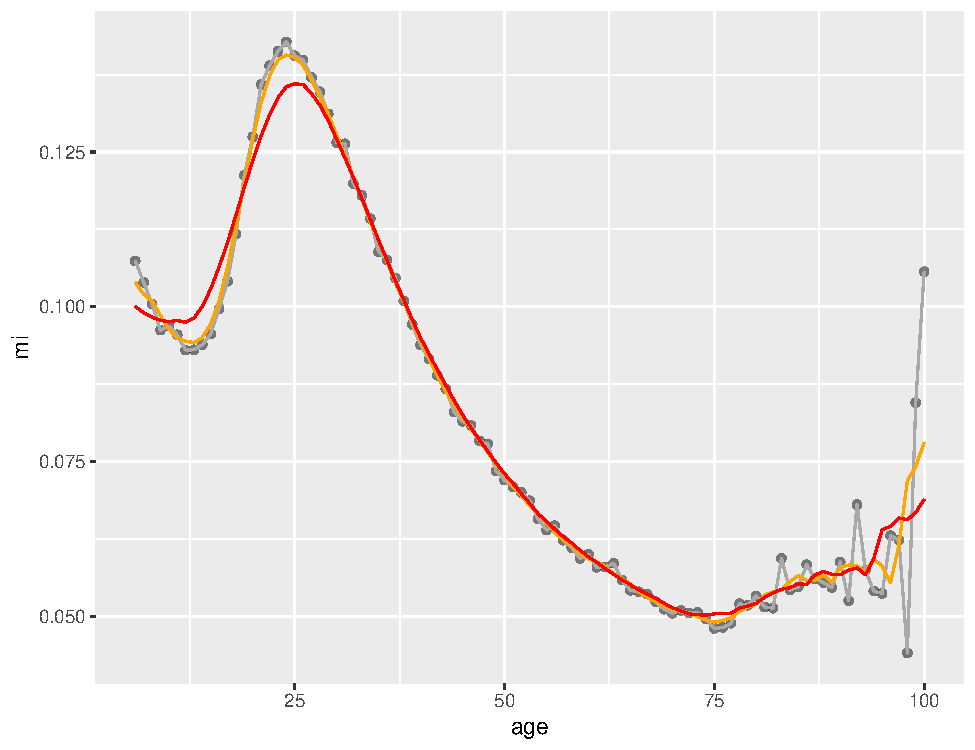
\includegraphics{_main_files/figure-latex/unnamed-chunk-100-1.pdf}

\hypertarget{loess-smoothing}{%
\subsection{Loess smoothing}\label{loess-smoothing}}

\begin{itemize}
\tightlist
\item
  The \texttt{loess.smooth} function is also unlikely to smooth a migration age schedule as the default span parameter is too small

  \begin{itemize}
  \tightlist
  \item
    Adjust the smoothing parameter using \texttt{spar} (between 0 and 1), default is \texttt{2/3}
  \item
    Use \texttt{evaluation} to set the number of predicted values
  \end{itemize}
\end{itemize}

\begin{Shaded}
\begin{Highlighting}[]
\NormalTok{b }\OtherTok{\textless{}{-}}\NormalTok{ b }\SpecialCharTok{\%\textgreater{}\%}
  \FunctionTok{mutate}\NormalTok{(}
    \AttributeTok{lo\_default =} \FunctionTok{loess.smooth}\NormalTok{(}\AttributeTok{x =}\NormalTok{ age, }\AttributeTok{y =}\NormalTok{ mi, }\AttributeTok{evaluation =} \FunctionTok{n}\NormalTok{())}\SpecialCharTok{$}\NormalTok{y,}
    \AttributeTok{lo\_sp2 =} \FunctionTok{loess.smooth}\NormalTok{(}\AttributeTok{x =}\NormalTok{ age, }\AttributeTok{y =}\NormalTok{ mi, }\AttributeTok{evaluation =} \FunctionTok{n}\NormalTok{(), }\AttributeTok{span =} \FloatTok{0.2}\NormalTok{)}\SpecialCharTok{$}\NormalTok{y,}
    \AttributeTok{lo\_sp1 =} \FunctionTok{loess.smooth}\NormalTok{(}\AttributeTok{x =}\NormalTok{ age, }\AttributeTok{y =}\NormalTok{ mi, }\AttributeTok{evaluation =} \FunctionTok{n}\NormalTok{(), }\AttributeTok{span =} \FloatTok{0.1}\NormalTok{)}\SpecialCharTok{$}\NormalTok{y,}
\NormalTok{  )}
\end{Highlighting}
\end{Shaded}

\hypertarget{loess-smoothing-1}{%
\subsection{Loess smoothing}\label{loess-smoothing-1}}

\begin{Shaded}
\begin{Highlighting}[]
\FunctionTok{ggplot}\NormalTok{(}\AttributeTok{data =}\NormalTok{ b, }
       \AttributeTok{mapping =} \FunctionTok{aes}\NormalTok{(}\AttributeTok{x =}\NormalTok{ age, }\AttributeTok{y =}\NormalTok{ mi)) }\SpecialCharTok{+}
  \FunctionTok{geom\_point}\NormalTok{(}\AttributeTok{alpha =} \FloatTok{0.5}\NormalTok{) }\SpecialCharTok{+} 
  \FunctionTok{geom\_line}\NormalTok{(}\AttributeTok{mapping =} \FunctionTok{aes}\NormalTok{(}\AttributeTok{y =}\NormalTok{ lo\_default), }\AttributeTok{col =} \StringTok{"darkgrey"}\NormalTok{) }\SpecialCharTok{+}
  \FunctionTok{geom\_line}\NormalTok{(}\AttributeTok{mapping =} \FunctionTok{aes}\NormalTok{(}\AttributeTok{y =}\NormalTok{ lo\_sp2), }\AttributeTok{col =} \StringTok{"orange"}\NormalTok{) }\SpecialCharTok{+}
  \FunctionTok{geom\_line}\NormalTok{(}\AttributeTok{mapping =} \FunctionTok{aes}\NormalTok{(}\AttributeTok{y =}\NormalTok{ lo\_sp1), }\AttributeTok{col =} \StringTok{"red"}\NormalTok{)}
\end{Highlighting}
\end{Shaded}

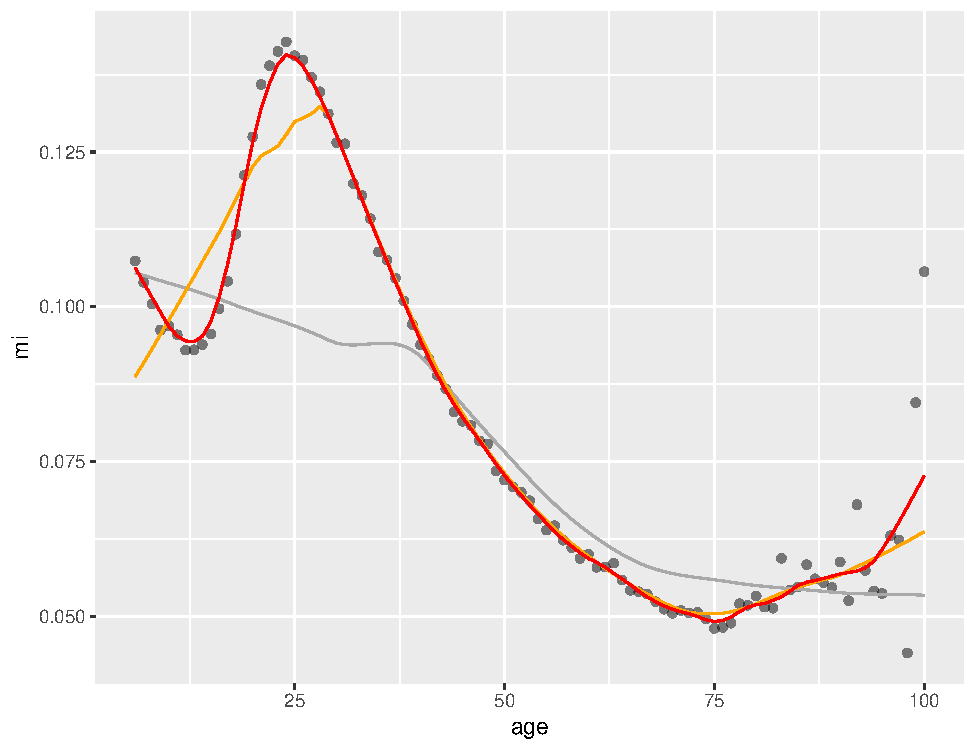
\includegraphics{_main_files/figure-latex/unnamed-chunk-102-1.pdf}

\hypertarget{cubic-spline-smoothing}{%
\subsection{Cubic spline smoothing}\label{cubic-spline-smoothing}}

\begin{itemize}
\tightlist
\item
  The \texttt{smooth.spline} function might have a nice smooth fit to migration age schedule

  \begin{itemize}
  \tightlist
  \item
    Adjust the smoothing parameter using \texttt{spar} (between 0 and 1)
  \item
    Use \texttt{n} to set the number of predicted values
  \end{itemize}
\end{itemize}

\begin{Shaded}
\begin{Highlighting}[]
\NormalTok{b }\OtherTok{\textless{}{-}}\NormalTok{ b }\SpecialCharTok{\%\textgreater{}\%}
  \FunctionTok{mutate}\NormalTok{(}
    \AttributeTok{s\_default =} \FunctionTok{smooth.spline}\NormalTok{(}\AttributeTok{x =}\NormalTok{ age, }\AttributeTok{y =}\NormalTok{ mi, }\AttributeTok{n =} \FunctionTok{n}\NormalTok{())}\SpecialCharTok{$}\NormalTok{y,}
    \AttributeTok{s\_sp6 =} \FunctionTok{smooth.spline}\NormalTok{(}\AttributeTok{x =}\NormalTok{ age, }\AttributeTok{y =}\NormalTok{ mi, }\AttributeTok{n =} \FunctionTok{n}\NormalTok{(), }\AttributeTok{spar =} \FloatTok{0.6}\NormalTok{)}\SpecialCharTok{$}\NormalTok{y,}
    \AttributeTok{s\_sp8 =} \FunctionTok{smooth.spline}\NormalTok{(}\AttributeTok{x =}\NormalTok{ age, }\AttributeTok{y =}\NormalTok{ mi, }\AttributeTok{n =} \FunctionTok{n}\NormalTok{(), }\AttributeTok{spar =} \FloatTok{0.8}\NormalTok{)}\SpecialCharTok{$}\NormalTok{y)}
\end{Highlighting}
\end{Shaded}

\hypertarget{cubic-spline-smoothing-1}{%
\subsection{Cubic spline smoothing}\label{cubic-spline-smoothing-1}}

\begin{Shaded}
\begin{Highlighting}[]
\FunctionTok{ggplot}\NormalTok{(}\AttributeTok{data =}\NormalTok{ b, }
       \AttributeTok{mapping =} \FunctionTok{aes}\NormalTok{(}\AttributeTok{x =}\NormalTok{ age, }\AttributeTok{y =}\NormalTok{ mi)) }\SpecialCharTok{+}
  \FunctionTok{geom\_point}\NormalTok{(}\AttributeTok{alpha =} \FloatTok{0.5}\NormalTok{) }\SpecialCharTok{+} 
  \FunctionTok{geom\_line}\NormalTok{(}\AttributeTok{mapping =} \FunctionTok{aes}\NormalTok{(}\AttributeTok{y =}\NormalTok{ s\_default), }\AttributeTok{col =} \StringTok{"darkgrey"}\NormalTok{) }\SpecialCharTok{+}
  \FunctionTok{geom\_line}\NormalTok{(}\AttributeTok{mapping =} \FunctionTok{aes}\NormalTok{(}\AttributeTok{y =}\NormalTok{ s\_sp6), }\AttributeTok{col =} \StringTok{"orange"}\NormalTok{) }\SpecialCharTok{+} 
  \FunctionTok{geom\_line}\NormalTok{(}\AttributeTok{mapping =} \FunctionTok{aes}\NormalTok{(}\AttributeTok{y =}\NormalTok{ s\_sp8), }\AttributeTok{col =} \StringTok{"red"}\NormalTok{)}
\end{Highlighting}
\end{Shaded}

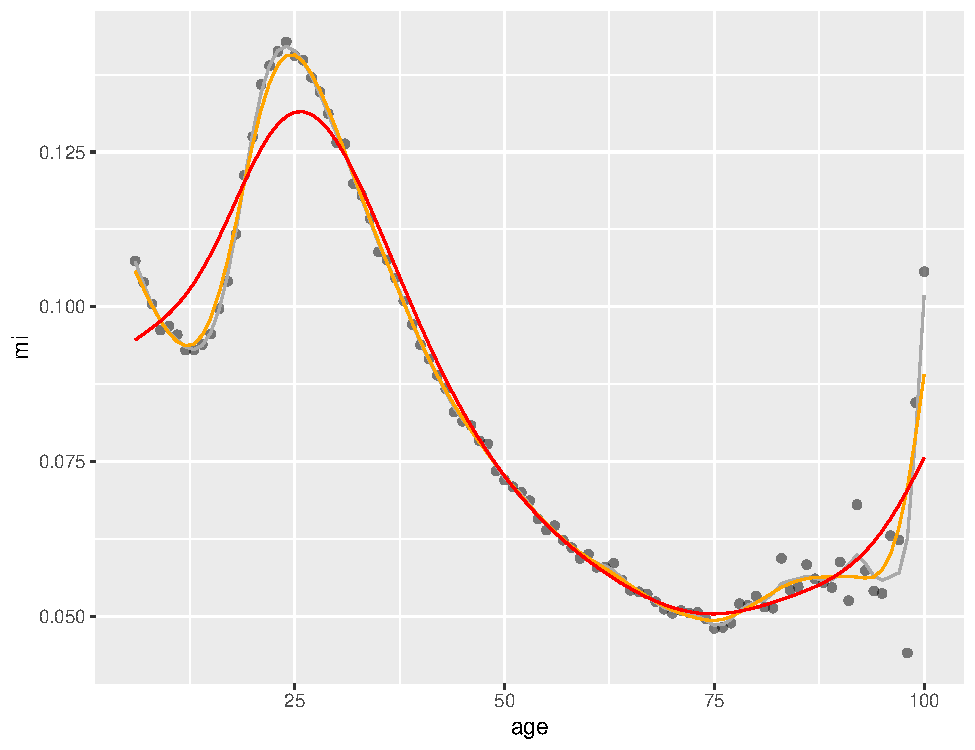
\includegraphics{_main_files/figure-latex/unnamed-chunk-104-1.pdf}

\hypertarget{graduating}{%
\section{Graduating}\label{graduating}}

\hypertarget{graduating-1}{%
\subsection{Graduating}\label{graduating-1}}

\begin{itemize}
\tightlist
\item
  If you require single year migration age data, but only have data by age groups, then graduating methods can be used to estimate migration for each age that sum to the reported age group totals.
\item
  There a multiple graduating methods available in the \texttt{graduate()} function in the DemoTools package

  \begin{itemize}
  \tightlist
  \item
    Built for interpolating population totals, but also suitable for migration flows
  \item
    See the \href{https://timriffe.github.io/DemoTools/articles/graduation_with_demotools.html}{guide} for more detail on different methods
  \end{itemize}
\item
  Requires users to provide \texttt{Value} and minimum \texttt{Age}.
\item
  Can also specify the maximum value of final open age group, if exists, for certain methods such as \texttt{pclm}.
\end{itemize}

\hypertarget{graduating-2}{%
\subsection{Graduating}\label{graduating-2}}

\begin{itemize}
\tightlist
\item
  Using the out-migration to Italian islands area in 1970
\end{itemize}

\begin{Shaded}
\begin{Highlighting}[]
\FunctionTok{head}\NormalTok{(i)}
\end{Highlighting}
\end{Shaded}

\begin{verbatim}
## # A tibble: 6 x 8
## # Groups:   age_grp [6]
##   age_grp age_min age_max region  in_mig out_mig  turn   net
##   <fct>     <int>   <int> <chr>    <dbl>   <dbl> <dbl> <dbl>
## 1 0-4           0       4 Islands   4532    7876 12408 -3344
## 2 5-9           5       9 Islands   3592    7271 10863 -3679
## 3 10-14        10      14 Islands   2228    5779  8007 -3551
## 4 15-19        15      19 Islands   3064    8526 11590 -5462
## 5 20-24        20      24 Islands   6861   15629 22490 -8768
## 6 25-29        25      29 Islands   5891   11224 17115 -5333
\end{verbatim}

\begin{Shaded}
\begin{Highlighting}[]
\NormalTok{mx }\OtherTok{\textless{}{-}} \FunctionTok{graduate}\NormalTok{(}\AttributeTok{Value =}\NormalTok{ i}\SpecialCharTok{$}\NormalTok{out\_mig, }\AttributeTok{Age =}\NormalTok{ i}\SpecialCharTok{$}\NormalTok{age\_min, }
               \AttributeTok{method =} \StringTok{"pclm"}\NormalTok{, }\AttributeTok{OAG =}  \ConstantTok{TRUE}\NormalTok{, }\AttributeTok{OAnew =} \DecValTok{100}\NormalTok{)}
\NormalTok{mx}
\end{Highlighting}
\end{Shaded}

\begin{verbatim}
##           0           1           2           3           4           5 
## 1540.822616 1563.081967 1582.487050 1594.810184 1594.859870 1576.283303 
##           6           7           8           9          10          11 
## 1534.233098 1470.025351 1388.679355 1301.771896 1221.108012 1158.023181 
##          12          13          14          15          16          17 
## 1121.942083 1119.554144 1158.435391 1247.103598 1398.284195 1623.913611 
##          18          19          20          21          22          23 
## 1935.092918 2321.755623 2741.539266 3112.329630 3324.796748 3324.915552 
##          24          25          26          27          28          29 
## 3125.320990 2812.139216 2482.216694 2189.772149 1958.656025 1781.415216 
##          30          31          32          33          34          35 
## 1641.408137 1521.553492 1407.170481 1293.744997 1182.104397 1077.109503 
##          36          37          38          39          40          41 
##  984.353885  906.668010  845.151088  798.771354  765.545510  742.411329 
##          42          43          44          45          46          47 
##  725.616964  710.186702  690.289756  660.651697  617.401802  562.289211 
##          48          49          50          51          52          53 
##  501.033932  441.541294  391.355174  354.054434  330.929904  320.470746 
##          54          55          56          57          58          59 
##  319.333087  323.280116  326.437894  324.340533  314.694694  298.140366 
##          60          61          62          63          64          65 
##  278.157544  258.006157  240.321118  226.037262  214.561457  204.846583 
##          66          67          68          69          70          71 
##  195.376275  185.304981  174.609045  163.809589  153.997862  145.822900 
##          72          73          74          75          76          77 
##  139.398446  134.182156  128.693201  121.517548  111.497757   98.816336 
##          78          79          80          81          82          83 
##   85.271323   72.734621   62.959243   56.411258   52.462550   49.962470 
##          84          85          86          87          88          89 
##   46.549791   40.446619   31.418669   21.471299   13.559411    8.503983 
##          90          91          92          93          94          95 
##    5.890223    4.961916    5.352577    7.481251   12.438906   21.715730 
##          96          97          98          99         100 
##   32.832828   36.073090   26.875823   13.368895    4.891892
\end{verbatim}

\hypertarget{graduating-3}{%
\subsection{Graduating}\label{graduating-3}}

\begin{Shaded}
\begin{Highlighting}[]
\CommentTok{\# check for close match between graduate values and out\_mig }
\CommentTok{\# 0{-}4}
\FunctionTok{sum}\NormalTok{(mx[}\DecValTok{1}\SpecialCharTok{:}\DecValTok{5}\NormalTok{])}
\end{Highlighting}
\end{Shaded}

\begin{verbatim}
## [1] 7876.062
\end{verbatim}

\begin{Shaded}
\begin{Highlighting}[]
\CommentTok{\# 5{-}9}
\FunctionTok{sum}\NormalTok{(mx[}\DecValTok{6}\SpecialCharTok{:}\DecValTok{10}\NormalTok{])}
\end{Highlighting}
\end{Shaded}

\begin{verbatim}
## [1] 7270.993
\end{verbatim}

\begin{Shaded}
\begin{Highlighting}[]
\FunctionTok{select}\NormalTok{(i, age\_grp, out\_mig)}
\end{Highlighting}
\end{Shaded}

\begin{verbatim}
## # A tibble: 20 x 2
## # Groups:   age_grp [20]
##    age_grp out_mig
##    <fct>     <dbl>
##  1 0-4        7876
##  2 5-9        7271
##  3 10-14      5779
##  4 15-19      8526
##  5 20-24     15629
##  6 25-29     11224
##  7 30-34      7046
##  8 35-39      4612
##  9 40-44      3634
## 10 45-49      2783
## 11 50-54      1716
## 12 55-59      1587
## 13 60-64      1217
## 14 65-69       924
## 15 70-74       702
## 16 75-79       490
## 17 80-84       268
## 18 85-89       116
## 19 90-94        35
## 20 95+         137
\end{verbatim}

\hypertarget{graduating-4}{%
\subsection{Graduating}\label{graduating-4}}

\begin{Shaded}
\begin{Highlighting}[]
\CommentTok{\# different scales in y{-}axis}
\FunctionTok{ggplot}\NormalTok{(}\AttributeTok{data =}\NormalTok{ i, }
       \AttributeTok{mapping =} \FunctionTok{aes}\NormalTok{(}\AttributeTok{x =}\NormalTok{ age\_min }\SpecialCharTok{+} \FloatTok{2.5}\NormalTok{, }\AttributeTok{y =}\NormalTok{ out\_mig)) }\SpecialCharTok{+}
  \FunctionTok{geom\_point}\NormalTok{()}

\FunctionTok{tibble}\NormalTok{(}\AttributeTok{age =} \DecValTok{0}\SpecialCharTok{:}\DecValTok{100}\NormalTok{, }\AttributeTok{mx =}\NormalTok{ mx) }\SpecialCharTok{\%\textgreater{}\%}
  \FunctionTok{ggplot}\NormalTok{(}\AttributeTok{mapping =} \FunctionTok{aes}\NormalTok{(}\AttributeTok{x =}\NormalTok{ age, }\AttributeTok{y =}\NormalTok{ mx)) }\SpecialCharTok{+}
  \FunctionTok{geom\_line}\NormalTok{()}
\end{Highlighting}
\end{Shaded}

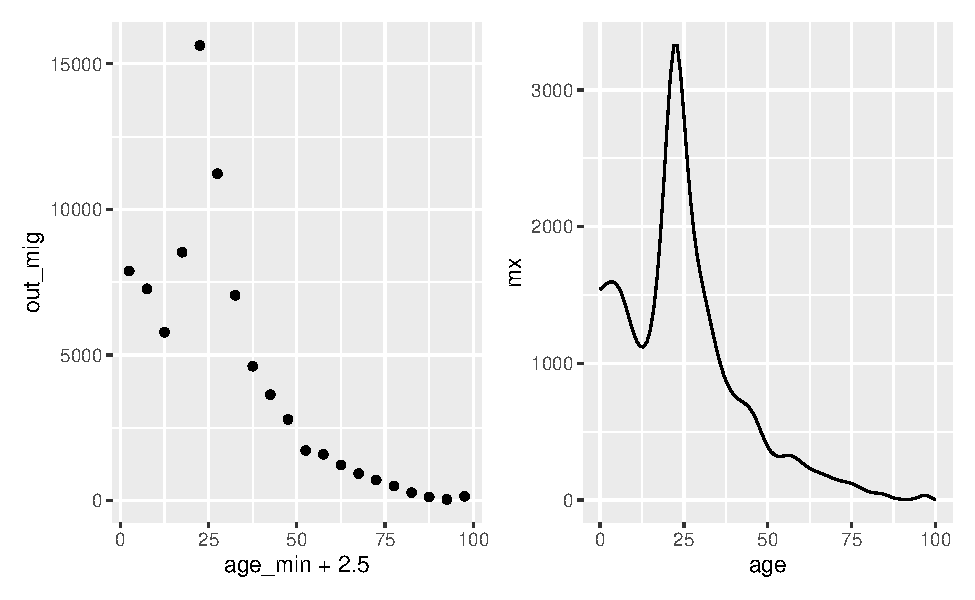
\includegraphics{_main_files/figure-latex/unnamed-chunk-108-1.pdf}

\hypertarget{exercise-5-ex5.r}{%
\subsection{Exercise 5 (ex5.R)}\label{exercise-5-ex5.r}}

\begin{Shaded}
\begin{Highlighting}[]
\CommentTok{\# 0.  a) Load the KOSTAT2021.Rproj file. }
\CommentTok{\#     Run the getwd() below. It should print the directory where the }
\CommentTok{\#     KOSTAT2021.Rproj file is located.}
\FunctionTok{getwd}\NormalTok{()}
\CommentTok{\#     b) Load the packages used in this exercise}
\FunctionTok{library}\NormalTok{(tidyverse)}
\FunctionTok{library}\NormalTok{(migest)}
\FunctionTok{library}\NormalTok{(DemoTools)}
\DocumentationTok{\#\#}
\DocumentationTok{\#\#}
\DocumentationTok{\#\#}
\CommentTok{\# 1. Run the code below to read in the population age structure data for flows}
\CommentTok{\#    from Florida to New York based on the 2015 American Community Survey}
\NormalTok{flny }\OtherTok{\textless{}{-}} \FunctionTok{read\_csv}\NormalTok{(}\StringTok{"./data/florida\_new\_york\_acs\_2015.csv"}\NormalTok{)}
\NormalTok{flny}
\CommentTok{\# 2. Run the code below to plot the age schedule for migration from New York to }
\CommentTok{\#    Florida. Note, the uneven spread of the age groups}
\FunctionTok{ggplot}\NormalTok{(}\AttributeTok{data =}\NormalTok{ x, }\AttributeTok{mapping =} \FunctionTok{aes}\NormalTok{(}\AttributeTok{x =}\NormalTok{ AGE\_label, }\AttributeTok{y =}\NormalTok{ mig\_in, }\AttributeTok{group =} \DecValTok{1}\NormalTok{)) }\SpecialCharTok{+}
  \FunctionTok{geom\_point}\NormalTok{() }\SpecialCharTok{+}
  \FunctionTok{geom\_line}\NormalTok{() }\SpecialCharTok{+}
  \FunctionTok{theme}\NormalTok{(}\AttributeTok{axis.text =} \FunctionTok{element\_text}\NormalTok{(}\AttributeTok{angle =} \DecValTok{45}\NormalTok{, }\AttributeTok{hjust =} \DecValTok{1}\NormalTok{))}
\CommentTok{\# 3. Estimate the age schedule based on single years up to 100, based on a }
\CommentTok{\#    graduation of the migration data in flny}
\NormalTok{mx }\OtherTok{\textless{}{-}} \DocumentationTok{\#\#\#\#\#(Value = flny$\#\#\#\#\#, Age = \#\#\#\#\#$age\_min, }
\NormalTok{               method }\OtherTok{=} \StringTok{"pclm"}\NormalTok{, OAG }\OtherTok{=}  \ConstantTok{TRUE}\NormalTok{, OAnew }\OtherTok{=} \DocumentationTok{\#\#\#\#\#)}
\NormalTok{mx}
\CommentTok{\# 4. Build a data frame to store the graduated data frame and a migration }
\CommentTok{\#    intensities (mx rescaled so that age specific intensities sum to one)}
\NormalTok{d }\OtherTok{\textless{}{-}} \FunctionTok{tibble}\NormalTok{(}
  \AttributeTok{age =} \DecValTok{1}\SpecialCharTok{:}\DecValTok{100}\NormalTok{, }
  \AttributeTok{mx =}\NormalTok{ mx,}
  \AttributeTok{mi =} \DocumentationTok{\#\#\#\#\#/sum(mx)}
\NormalTok{)}
\NormalTok{d}
\CommentTok{\# 5. Plot the graduated age schedule }
\NormalTok{d }\SpecialCharTok{\%\textgreater{}\%}
  \FunctionTok{ggplot}\NormalTok{(}\AttributeTok{mapping =} \FunctionTok{aes}\NormalTok{(}\AttributeTok{x =} \DocumentationTok{\#\#\#\#\#, y = \#\#\#\#\#)) +}
  \FunctionTok{geom\_line}\NormalTok{()}
\CommentTok{\# 6. Use the age and migration intensities in d to fit a 11 parameter Rogers{-}}
\CommentTok{\#    Castro age schedule (with a retirement peak, but no post retirement peak)}
\NormalTok{f }\OtherTok{\textless{}{-}} \FunctionTok{mig\_estimate\_rc}\NormalTok{(}\AttributeTok{ages =}\NormalTok{ d}\SpecialCharTok{$}\DocumentationTok{\#\#\#\#\#, mx = d$mi,}
                     \AttributeTok{pre\_working\_age =} \DocumentationTok{\#\#\#\#\#, working\_age = TRUE,}
                     \AttributeTok{retirement =} \DocumentationTok{\#\#\#\#\#, post\_retirement = FALSE)}
\CommentTok{\# 7. Run the code below to plot the fitted Rogers Casto age schedule}
\FunctionTok{ggplot}\NormalTok{(}\AttributeTok{data =}\NormalTok{ f[[}\DecValTok{2}\NormalTok{]],}
       \AttributeTok{mapping =} \FunctionTok{aes}\NormalTok{(}\AttributeTok{x =}\NormalTok{ age, }\AttributeTok{y =}\NormalTok{ data)) }\SpecialCharTok{+}
  \FunctionTok{geom\_ribbon}\NormalTok{(}\AttributeTok{mapping =} \FunctionTok{aes}\NormalTok{(}\AttributeTok{ymin =}\NormalTok{ lower, }\AttributeTok{ymax =}\NormalTok{ upper), }\AttributeTok{fill =} \StringTok{"lightblue"}\NormalTok{) }\SpecialCharTok{+}
  \FunctionTok{geom\_line}\NormalTok{(}\AttributeTok{mapping =} \FunctionTok{aes}\NormalTok{(}\AttributeTok{y =}\NormalTok{ median), }\AttributeTok{colour =} \StringTok{"blue"}\NormalTok{) }\SpecialCharTok{+}
  \FunctionTok{geom\_point}\NormalTok{()}
\CommentTok{\# 8. Calculate the indices based on the median of the parameter distributions }
\CommentTok{\#    for the Rogers Castro age schedule}
\NormalTok{f[[}\DecValTok{1}\NormalTok{]] }\SpecialCharTok{\%\textgreater{}\%}
  \FunctionTok{select}\NormalTok{(variable, median) }\SpecialCharTok{\%\textgreater{}\%}
  \DocumentationTok{\#\#\#\#\#() \%\textgreater{}\%}
  \DocumentationTok{\#\#\#\#\#()}
\end{Highlighting}
\end{Shaded}

\hypertarget{describing-bilteral-migration-data}{%
\chapter{Describing Bilteral Migration Data}\label{describing-bilteral-migration-data}}

\hypertarget{components}{%
\section{Components}\label{components}}

\hypertarget{multiplicative-component-model}{%
\subsection{Multiplicative Component Model}\label{multiplicative-component-model}}

\begin{itemize}
\tightlist
\item
  \citet{rogers2002dms} proposed dis-aggregating origin-destination flow tables into separate components to allow for an easier examination of migration flows

  \begin{itemize}
  \tightlist
  \item
    Overall component - level of migration \(\gamma\)
  \item
    Origin component - relative `pushes' from each region \(\alpha_i\)
  \item
    Destination component - relative `pulls' to each region \(\beta_j\)
  \item
    Origin--Destination interaction component - physical or social distance between places not explained by the overall and main effects. \(\delta_{ij}\)
  \end{itemize}
\item
  Simple calculations to estimate each component:
  \[
  \gamma = m_{++} \qquad \alpha_i = \dfrac{m_{i+}}{m_{++}} \qquad \beta_j = \dfrac{m_{+j}}{m_{++}} \qquad  \delta_{ij} = \dfrac{m_{ij}}{\gamma\alpha_i\beta_j}
  \]
\item
  The interaction, \(\delta_{ij}\), is the ratio of observed flow to an expected flow (for the case of no interaction).
\end{itemize}

\hypertarget{multiplicative-component-model-1}{%
\subsection{Multiplicative Component Model}\label{multiplicative-component-model-1}}

\begin{itemize}
\tightlist
\item
  The dis-aggregation of the components is multiplicative:
  \[
  m_{ij} = \gamma \alpha_i \beta_j \delta_{ij}
  \]
\item
  Equivalent to a saturated Poisson regression model (\(R^2 = 1\)) where

  \begin{itemize}
  \tightlist
  \item
    \(\gamma\) is constant term
  \item
    \(\alpha_i\) is categorical term for the origin regions
  \item
    \(\beta_j\) is categorical term for the destination regions
  \item
    \(\delta_{ij}\) is an interaction term between the \(\alpha_i\) and \(\beta_j\)
    \[
    \log m_{ij} = \gamma +  \alpha_i ORIG_i + \beta_j DEST_j +  \delta_i ORIG_i:DEST_j
    \]
  \end{itemize}
\item
  When data is in a tidy format with row \(h\) would be:
  \[
  \log y_{h} =  \beta_0 +  \beta_1 ORIG_{h} + \beta_2 DEST_{h} + \beta_3 ORIG_{h}:DEST_{h}
  \]
\item
  Poisson regression models such as these - where all the predictor variables are categorical - are also know as log-linear models
\item
  Standard functions for fitting regression models, such as \texttt{glm()} in R will provide the same fitted values, but different parameter estimates

  \begin{itemize}
  \tightlist
  \item
    Use different coding system for the constraints when estimating parameters
  \item
    Rogers' terms the parameter estimates using the equations for \(\gamma, \alpha_i, \beta_j\) and \(\delta_{ij}\) above the \emph{total reference} coding system
  \end{itemize}
\end{itemize}

\hypertarget{multiplicative-component-model-2}{%
\subsection{Multiplicative Component Model}\label{multiplicative-component-model-2}}

\begin{itemize}
\tightlist
\item
  The \emph{migest} package contains a \texttt{multi\_comp()} function to generate parameter estimates from an origin-destination flow matrix

  \begin{itemize}
  \tightlist
  \item
    Demonstrate with previous dummy data set
  \end{itemize}
\end{itemize}

\begin{Shaded}
\begin{Highlighting}[]
\NormalTok{r }\OtherTok{\textless{}{-}}\NormalTok{ LETTERS[}\DecValTok{1}\SpecialCharTok{:}\DecValTok{4}\NormalTok{]}
\NormalTok{m0 }\OtherTok{\textless{}{-}} \FunctionTok{matrix}\NormalTok{(}\AttributeTok{data =} \FunctionTok{c}\NormalTok{(}\DecValTok{0}\NormalTok{, }\DecValTok{100}\NormalTok{, }\DecValTok{30}\NormalTok{, }\DecValTok{70}\NormalTok{, }
                      \DecValTok{50}\NormalTok{, }\DecValTok{0}\NormalTok{, }\DecValTok{45}\NormalTok{, }\DecValTok{5}\NormalTok{, }
                      \DecValTok{60}\NormalTok{, }\DecValTok{35}\NormalTok{, }\DecValTok{0}\NormalTok{, }\DecValTok{40}\NormalTok{, }
                      \DecValTok{20}\NormalTok{, }\DecValTok{25}\NormalTok{, }\DecValTok{20}\NormalTok{, }\DecValTok{0}\NormalTok{), }
             \AttributeTok{nrow =} \DecValTok{4}\NormalTok{, }\AttributeTok{ncol =} \DecValTok{4}\NormalTok{, }\AttributeTok{byrow =} \ConstantTok{TRUE}\NormalTok{, }
             \AttributeTok{dimnames =} \FunctionTok{list}\NormalTok{(}\AttributeTok{orig =}\NormalTok{ r, }\AttributeTok{dest =}\NormalTok{ r))}
\FunctionTok{addmargins}\NormalTok{(m0)}
\end{Highlighting}
\end{Shaded}

\begin{verbatim}
##      dest
## orig    A   B  C   D Sum
##   A     0 100 30  70 200
##   B    50   0 45   5 100
##   C    60  35  0  40 135
##   D    20  25 20   0  65
##   Sum 130 160 95 115 500
\end{verbatim}

\hypertarget{multiplicative-component-model-3}{%
\subsection{Multiplicative Component Model}\label{multiplicative-component-model-3}}

\begin{Shaded}
\begin{Highlighting}[]
\FunctionTok{library}\NormalTok{(tidyverse)}
\FunctionTok{library}\NormalTok{(migest)}
\NormalTok{m0 }\SpecialCharTok{\%\textgreater{}\%}
  \FunctionTok{multi\_comp}\NormalTok{() }\SpecialCharTok{\%\textgreater{}\%}
  \FunctionTok{round}\NormalTok{(}\DecValTok{3}\NormalTok{)}
\end{Highlighting}
\end{Shaded}

\begin{verbatim}
##      dest
## orig        A       B       C       D     Sum
##   A     0.000   1.563   0.789   1.522   0.400
##   B     1.923   0.000   2.368   0.217   0.200
##   C     1.709   0.810   0.000   1.288   0.270
##   D     1.183   1.202   1.619   0.000   0.130
##   Sum   0.260   0.320   0.190   0.230 500.000
\end{verbatim}

\hypertarget{multiplicative-component-model-4}{%
\subsection{Multiplicative Component Model}\label{multiplicative-component-model-4}}

\begin{itemize}
\tightlist
\item
  As the model is saturated, the fitted values are the same as the observed values.
\end{itemize}

\begin{Shaded}
\begin{Highlighting}[]
\FunctionTok{multi\_comp}\NormalTok{(}\AttributeTok{m =}\NormalTok{ m0)}
\end{Highlighting}
\end{Shaded}

\begin{verbatim}
##      dest
## orig            A           B           C           D         Sum
##   A     0.0000000   1.5625000   0.7894737   1.5217391   0.4000000
##   B     1.9230769   0.0000000   2.3684211   0.2173913   0.2000000
##   C     1.7094017   0.8101852   0.0000000   1.2882448   0.2700000
##   D     1.1834320   1.2019231   1.6194332   0.0000000   0.1300000
##   Sum   0.2600000   0.3200000   0.1900000   0.2300000 500.0000000
\end{verbatim}

\begin{Shaded}
\begin{Highlighting}[]
\CommentTok{\# fitted value for A to B}
\DecValTok{500} \SpecialCharTok{*} \FloatTok{0.4} \SpecialCharTok{*} \FloatTok{0.32} \SpecialCharTok{*} \FloatTok{1.5625}
\end{Highlighting}
\end{Shaded}

\begin{verbatim}
## [1] 100
\end{verbatim}

\hypertarget{multiplicative-component-model-5}{%
\subsection{Multiplicative Component Model}\label{multiplicative-component-model-5}}

\begin{itemize}
\tightlist
\item
  The total reference coding scheme for the parameter estimates are easier to examine than parameter estimates from a Poisson model fitted using \texttt{glm()}

  \begin{itemize}
  \tightlist
  \item
    More detail on \texttt{glm()} in next section
  \end{itemize}
\end{itemize}

\begin{Shaded}
\begin{Highlighting}[]
\NormalTok{d0 }\OtherTok{\textless{}{-}} \FunctionTok{as.data.frame.table}\NormalTok{(}\AttributeTok{x =}\NormalTok{ m0, }\AttributeTok{responseName =} \StringTok{"flow"}\NormalTok{)}
\NormalTok{f0 }\OtherTok{\textless{}{-}} \FunctionTok{glm}\NormalTok{(}\AttributeTok{formula =}\NormalTok{ flow }\SpecialCharTok{\textasciitilde{}}\NormalTok{ orig }\SpecialCharTok{+}\NormalTok{ dest }\SpecialCharTok{+}\NormalTok{ orig }\SpecialCharTok{*}\NormalTok{ dest, }\AttributeTok{family =} \FunctionTok{poisson}\NormalTok{(), }
           \AttributeTok{data =}\NormalTok{ d0)}
\NormalTok{f0}
\end{Highlighting}
\end{Shaded}

\begin{verbatim}
## 
## Call:  glm(formula = flow ~ orig + dest + orig * dest, family = poisson(), 
##     data = d0)
## 
## Coefficients:
## (Intercept)        origB        origC        origD        destB        destC  
##      -24.30        28.21        28.40        27.30        28.91        27.70  
##       destD  origB:destB  origC:destB  origD:destB  origB:destC  origC:destC  
##       28.55       -57.12       -29.45       -28.68       -27.81       -56.10  
## origD:destC  origB:destD  origC:destD  origD:destD  
##      -27.70       -30.85       -28.96       -55.85  
## 
## Degrees of Freedom: 15 Total (i.e. Null);  0 Residual
## Null Deviance:       463.7 
## Residual Deviance: 2.232e-10     AIC: 96.27
\end{verbatim}

\hypertarget{multiplicative-component-model-6}{%
\subsection{Multiplicative Component Model}\label{multiplicative-component-model-6}}

\begin{Shaded}
\begin{Highlighting}[]
\CommentTok{\# fitted and observed values are the same}
\NormalTok{d0 }\SpecialCharTok{\%\textgreater{}\%} 
  \FunctionTok{as\_tibble}\NormalTok{() }\SpecialCharTok{\%\textgreater{}\%}
  \FunctionTok{mutate}\NormalTok{(}\AttributeTok{fit =} \FunctionTok{round}\NormalTok{(f0}\SpecialCharTok{$}\NormalTok{fitted.values, }\AttributeTok{digits =} \DecValTok{5}\NormalTok{))}
\end{Highlighting}
\end{Shaded}

\begin{verbatim}
## # A tibble: 16 x 4
##    orig  dest   flow   fit
##    <fct> <fct> <dbl> <dbl>
##  1 A     A         0     0
##  2 B     A        50    50
##  3 C     A        60    60
##  4 D     A        20    20
##  5 A     B       100   100
##  6 B     B         0     0
##  7 C     B        35    35
##  8 D     B        25    25
##  9 A     C        30    30
## 10 B     C        45    45
## 11 C     C         0     0
## 12 D     C        20    20
## 13 A     D        70    70
## 14 B     D         5     5
## 15 C     D        40    40
## 16 D     D         0     0
\end{verbatim}

\hypertarget{multiplicative-component-model-7}{%
\subsection{Multiplicative Component Model}\label{multiplicative-component-model-7}}

\begin{itemize}
\tightlist
\item
  Rogers' and colleagues have used the multiplicative component model to estimate migration flow tables
\item
  Expand to multiple dimensions
\item
  Rectify bumpy age schedules

  \begin{itemize}
  \tightlist
  \item
    Replace reported age parameters (proportions) in the multiplicative component model with proportions from a more regular schedule.
  \item
    Multiply the new age parameters with the existing total, origin, destination and interaction parameters to obtain new estimated flows.
  \end{itemize}
\end{itemize}

\hypertarget{multiplicative-component-model-8}{%
\subsection{Multiplicative Component Model}\label{multiplicative-component-model-8}}

\begin{itemize}
\tightlist
\item
  Italian data in \emph{migest} package
\end{itemize}

\begin{Shaded}
\begin{Highlighting}[]
\NormalTok{italy\_area}
\end{Highlighting}
\end{Shaded}

\begin{verbatim}
## # A tibble: 3,500 x 5
##    orig       dest        year age_grp  flow
##    <chr>      <chr>      <dbl> <fct>   <dbl>
##  1 North-West North-West  1970 0-4         0
##  2 North-East North-West  1970 0-4      2350
##  3 Center     North-West  1970 0-4      1687
##  4 South      North-West  1970 0-4      9697
##  5 Islands    North-West  1970 0-4      5139
##  6 North-West North-East  1970 0-4      2448
##  7 North-East North-East  1970 0-4         0
##  8 Center     North-East  1970 0-4      1063
##  9 South      North-East  1970 0-4      1560
## 10 Islands    North-East  1970 0-4       689
## # ... with 3,490 more rows
\end{verbatim}

\hypertarget{multiplicative-component-model-9}{%
\subsection{Multiplicative Component Model}\label{multiplicative-component-model-9}}

\begin{Shaded}
\begin{Highlighting}[]
\CommentTok{\# single year, multiple age groups}
\NormalTok{c0 }\OtherTok{\textless{}{-}}\NormalTok{ italy\_area }\SpecialCharTok{\%\textgreater{}\%}
  \FunctionTok{filter}\NormalTok{(year }\SpecialCharTok{==} \DecValTok{2000}\NormalTok{) }\SpecialCharTok{\%\textgreater{}\%}
  \FunctionTok{multi\_comp}\NormalTok{()}
\FunctionTok{round}\NormalTok{(c0, }\DecValTok{3}\NormalTok{)}
\end{Highlighting}
\end{Shaded}

\begin{verbatim}
## , , age_grp = 0-4
## 
##             dest
## orig             Center    Islands North-East North-West      South        Sum
##   Center          0.000      1.401      0.859      0.909      2.370      0.010
##   Islands         0.970      0.000      1.181      1.513      0.681      0.012
##   North-East      1.053      1.916      0.000      1.179      2.501      0.010
##   North-West      0.877      2.490      0.887      0.000      2.023      0.014
##   South           1.409      0.531      1.184      1.102      0.000      0.025
##   Sum             0.016      0.007      0.017      0.018      0.014      0.072
## 
## , , age_grp = 5-9
## 
##             dest
## orig             Center    Islands North-East North-West      South        Sum
##   Center          0.000      1.589      0.779      0.762      2.243      0.007
##   Islands         1.166      0.000      1.393      1.707      0.562      0.010
##   North-East      0.840      1.932      0.000      0.936      2.085      0.006
##   North-West      0.877      2.714      0.844      0.000      1.963      0.010
##   South           1.387      0.507      1.283      1.151      0.000      0.018
##   Sum             0.011      0.005      0.012      0.012      0.009      0.050
## 
## , , age_grp = 10-14
## 
##             dest
## orig             Center    Islands North-East North-West      South        Sum
##   Center          0.000      1.570      0.738      0.667      1.978      0.005
##   Islands         1.333      0.000      1.572      1.791      0.463      0.008
##   North-East      0.861      1.834      0.000      0.840      1.805      0.004
##   North-West      0.793      2.694      0.826      0.000      1.959      0.007
##   South           1.424      0.411      1.332      1.226      0.000      0.014
##   Sum             0.009      0.004      0.010      0.009      0.006      0.037
## 
## , , age_grp = 15-19
## 
##             dest
## orig             Center    Islands North-East North-West      South        Sum
##   Center          0.000      1.358      0.732      0.668      1.673      0.005
##   Islands         1.261      0.000      1.617      2.109      0.417      0.009
##   North-East      0.677      1.769      0.000      0.847      1.697      0.004
##   North-West      0.629      2.606      0.818      0.000      1.803      0.007
##   South           1.449      0.347      1.449      1.340      0.000      0.016
##   Sum             0.009      0.004      0.011      0.011      0.006      0.041
## 
## , , age_grp = 20-24
## 
##             dest
## orig             Center    Islands North-East North-West      South        Sum
##   Center          0.000      1.044      0.852      0.759      1.552      0.014
##   Islands         0.983      0.000      1.490      1.948      0.436      0.025
##   North-East      0.593      1.530      0.000      0.852      1.808      0.012
##   North-West      0.533      1.880      0.726      0.000      1.449      0.018
##   South           1.419      0.425      1.788      1.624      0.000      0.055
##   Sum             0.025      0.009      0.036      0.037      0.017      0.124
## 
## , , age_grp = 25-29
## 
##             dest
## orig             Center    Islands North-East North-West      South        Sum
##   Center          0.000      1.092      0.992      0.939      2.093      0.027
##   Islands         0.915      0.000      1.221      1.599      0.544      0.034
##   North-East      0.910      1.420      0.000      1.161      1.829      0.023
##   North-West      0.795      1.652      0.947      0.000      1.719      0.034
##   South           1.473      0.482      1.457      1.373      0.000      0.079
##   Sum             0.044      0.014      0.053      0.054      0.032      0.197
## 
## , , age_grp = 30-34
## 
##             dest
## orig             Center    Islands North-East North-West      South        Sum
##   Center          0.000      1.211      1.088      1.159      2.136      0.025
##   Islands         0.915      0.000      1.053      1.390      0.526      0.025
##   North-East      1.143      1.384      0.000      1.362      1.837      0.021
##   North-West      0.945      1.857      1.091      0.000      1.756      0.031
##   South           1.544      0.445      1.205      1.244      0.000      0.059
##   Sum             0.039      0.012      0.040      0.043      0.027      0.160
## 
## , , age_grp = 35-39
## 
##             dest
## orig             Center    Islands North-East North-West      South        Sum
##   Center          0.000      1.439      1.175      1.245      2.126      0.016
##   Islands         0.956      0.000      1.073      1.372      0.407      0.015
##   North-East      1.278      1.396      0.000      1.484      1.719      0.013
##   North-West      1.158      2.026      1.229      0.000      1.753      0.020
##   South           1.465      0.424      1.089      1.085      0.000      0.032
##   Sum             0.024      0.008      0.024      0.025      0.015      0.096
## 
## , , age_grp = 40-44
## 
##             dest
## orig             Center    Islands North-East North-West      South        Sum
##   Center          0.000      1.547      1.283      1.266      2.200      0.009
##   Islands         1.001      0.000      1.090      1.445      0.367      0.008
##   North-East      1.322      1.563      0.000      1.417      1.626      0.007
##   North-West      1.234      2.353      1.261      0.000      1.885      0.012
##   South           1.317      0.354      1.044      1.001      0.000      0.017
##   Sum             0.013      0.005      0.014      0.014      0.009      0.054
## 
## , , age_grp = 45-49
## 
##             dest
## orig             Center    Islands North-East North-West      South        Sum
##   Center          0.000      1.638      1.130      1.204      2.331      0.005
##   Islands         1.076      0.000      1.100      1.372      0.400      0.005
##   North-East      1.406      1.701      0.000      1.501      1.607      0.005
##   North-West      1.320      2.600      1.354      0.000      2.007      0.008
##   South           1.286      0.408      0.919      0.912      0.000      0.010
##   Sum             0.008      0.003      0.008      0.008      0.006      0.033
## 
## , , age_grp = 50-54
## 
##             dest
## orig             Center    Islands North-East North-West      South        Sum
##   Center          0.000      1.887      1.064      1.110      2.579      0.005
##   Islands         0.997      0.000      0.861      1.226      0.361      0.004
##   North-East      1.449      1.709      0.000      1.505      1.541      0.004
##   North-West      1.519      3.174      1.595      0.000      2.391      0.008
##   South           1.267      0.366      0.738      0.831      0.000      0.007
##   Sum             0.007      0.003      0.006      0.006      0.005      0.028
## 
## , , age_grp = 55-59
## 
##             dest
## orig             Center    Islands North-East North-West      South        Sum
##   Center          0.000      2.263      1.084      1.029      2.894      0.004
##   Islands         0.845      0.000      0.643      1.027      0.343      0.003
##   North-East      1.448      1.641      0.000      1.455      1.391      0.003
##   North-West      1.724      3.929      1.892      0.000      2.921      0.008
##   South           1.160      0.398      0.544      0.722      0.000      0.005
##   Sum             0.006      0.003      0.005      0.005      0.005      0.023
## 
## , , age_grp = 60-64
## 
##             dest
## orig             Center    Islands North-East North-West      South        Sum
##   Center          0.000      2.271      1.067      1.084      3.282      0.004
##   Islands         0.767      0.000      0.397      0.933      0.414      0.002
##   North-East      1.331      1.473      0.000      1.578      1.500      0.003
##   North-West      1.633      4.038      1.938      0.000      3.047      0.008
##   South           1.245      0.395      0.444      0.734      0.000      0.005
##   Sum             0.005      0.003      0.004      0.004      0.005      0.022
## 
## , , age_grp = 65-69
## 
##             dest
## orig             Center    Islands North-East North-West      South        Sum
##   Center          0.000      2.383      1.159      1.030      3.451      0.003
##   Islands         0.827      0.000      0.435      0.876      0.385      0.002
##   North-East      1.222      1.237      0.000      1.629      1.439      0.002
##   North-West      1.518      3.324      1.891      0.000      2.933      0.005
##   South           1.340      0.479      0.419      0.874      0.000      0.004
##   Sum             0.004      0.002      0.003      0.004      0.004      0.017
## 
## , , age_grp = 70-74
## 
##             dest
## orig             Center    Islands North-East North-West      South        Sum
##   Center          0.000      2.409      0.999      1.353      3.269      0.003
##   Islands         0.723      0.000      0.381      1.253      0.385      0.002
##   North-East      1.301      1.200      0.000      1.765      1.113      0.002
##   North-West      1.421      2.608      1.719      0.000      2.445      0.004
##   South           1.451      0.432      0.460      1.065      0.000      0.004
##   Sum             0.004      0.001      0.003      0.004      0.003      0.014
## 
## , , age_grp = 75-79
## 
##             dest
## orig             Center    Islands North-East North-West      South        Sum
##   Center          0.000      1.926      1.174      1.311      2.957      0.003
##   Islands         0.819      0.000      0.352      1.352      0.431      0.002
##   North-East      1.395      0.840      0.000      2.114      0.929      0.002
##   North-West      1.327      2.463      1.810      0.000      1.963      0.003
##   South           1.450      0.437      0.488      1.173      0.000      0.004
##   Sum             0.003      0.001      0.003      0.004      0.002      0.013
## 
## , , age_grp = 80-84
## 
##             dest
## orig             Center    Islands North-East North-West      South        Sum
##   Center          0.000      1.846      1.070      1.503      2.636      0.002
##   Islands         0.804      0.000      0.428      1.295      0.519      0.001
##   North-East      1.466      0.631      0.000      2.117      0.986      0.001
##   North-West      1.232      2.001      1.825      0.000      1.826      0.002
##   South           1.571      0.408      0.493      1.258      0.000      0.003
##   Sum             0.002      0.001      0.002      0.002      0.001      0.008
## 
## , , age_grp = 85-89
## 
##             dest
## orig             Center    Islands North-East North-West      South        Sum
##   Center          0.000      1.545      1.509      1.606      2.575      0.001
##   Islands         0.739      0.000      0.383      1.345      0.414      0.001
##   North-East      1.766      1.254      0.000      2.809      0.913      0.001
##   North-West      1.090      1.667      1.944      0.000      1.395      0.002
##   South           1.410      0.301      0.415      1.240      0.000      0.002
##   Sum             0.002      0.000      0.001      0.002      0.001      0.007
## 
## , , age_grp = 90-94
## 
##             dest
## orig             Center    Islands North-East North-West      South        Sum
##   Center          0.000      1.319      1.211      1.906      2.277      0.001
##   Islands         0.809      0.000      0.418      1.033      0.359      0.000
##   North-East      1.469      1.083      0.000      2.835      0.660      0.000
##   North-West      1.494      1.635      2.216      0.000      1.778      0.001
##   South           1.452      0.250      0.387      1.142      0.000      0.001
##   Sum             0.001      0.000      0.001      0.001      0.000      0.003
## 
## , , age_grp = 95+
## 
##             dest
## orig             Center    Islands North-East North-West      South        Sum
##   Center          0.000      0.886      1.076      1.504      2.207      0.000
##   Islands         0.847      0.000      0.521      0.835      0.523      0.000
##   North-East      1.383      1.750      0.000      2.340      0.698      0.000
##   North-West      1.707      2.593      2.149      0.000      2.263      0.000
##   South           1.394      0.485      0.523      0.965      0.000      0.000
##   Sum             0.000      0.000      0.000      0.000      0.000      0.001
## 
## , , age_grp = Sum
## 
##             dest
## orig             Center    Islands North-East North-West      South        Sum
##   Center          0.000      0.017      0.037      0.039      0.054      0.148
##   Islands         0.038      0.000      0.048      0.067      0.013      0.166
##   North-East      0.030      0.016      0.000      0.041      0.037      0.125
##   North-West      0.045      0.037      0.056      0.000      0.063      0.202
##   South           0.120      0.013      0.111      0.115      0.000      0.360
##   Sum             0.233      0.084      0.253      0.263      0.168 277436.000
\end{verbatim}

\hypertarget{multiplicative-component-model-10}{%
\subsection{Multiplicative Component Model}\label{multiplicative-component-model-10}}

\begin{Shaded}
\begin{Highlighting}[]
\CommentTok{\# origin components (shares)}
\NormalTok{c0 }\SpecialCharTok{\%\textgreater{}\%}
  \FunctionTok{as.data.frame.table}\NormalTok{(}\AttributeTok{responseName =} \StringTok{"comp"}\NormalTok{) }\SpecialCharTok{\%\textgreater{}\%}
  \FunctionTok{filter}\NormalTok{(orig }\SpecialCharTok{!=} \StringTok{"Sum"}\NormalTok{, dest }\SpecialCharTok{==} \StringTok{"Sum"}\NormalTok{, age\_grp }\SpecialCharTok{==} \StringTok{"Sum"}\NormalTok{)}
\end{Highlighting}
\end{Shaded}

\begin{verbatim}
##         orig dest age_grp      comp
## 1     Center  Sum     Sum 0.1477314
## 2    Islands  Sum     Sum 0.1663483
## 3 North-East  Sum     Sum 0.1245945
## 4 North-West  Sum     Sum 0.2017835
## 5      South  Sum     Sum 0.3595424
\end{verbatim}

\begin{Shaded}
\begin{Highlighting}[]
\CommentTok{\# destination components (shares)}
\NormalTok{c0 }\SpecialCharTok{\%\textgreater{}\%}
  \FunctionTok{as.data.frame.table}\NormalTok{(}\AttributeTok{responseName =} \StringTok{"comp"}\NormalTok{) }\SpecialCharTok{\%\textgreater{}\%}
  \FunctionTok{filter}\NormalTok{(orig }\SpecialCharTok{==} \StringTok{"Sum"}\NormalTok{, dest }\SpecialCharTok{!=} \StringTok{"Sum"}\NormalTok{, age\_grp }\SpecialCharTok{==} \StringTok{"Sum"}\NormalTok{)}
\end{Highlighting}
\end{Shaded}

\begin{verbatim}
##   orig       dest age_grp       comp
## 1  Sum     Center     Sum 0.23305555
## 2  Sum    Islands     Sum 0.08368777
## 3  Sum North-East     Sum 0.25254113
## 4  Sum North-West     Sum 0.26283900
## 5  Sum      South     Sum 0.16787656
\end{verbatim}

\hypertarget{multiplicative-component-model-11}{%
\subsection{Multiplicative Component Model}\label{multiplicative-component-model-11}}

\begin{Shaded}
\begin{Highlighting}[]
\CommentTok{\# age components}
\NormalTok{c0 }\SpecialCharTok{\%\textgreater{}\%}
  \FunctionTok{as.data.frame.table}\NormalTok{(}\AttributeTok{responseName =} \StringTok{"comp"}\NormalTok{) }\SpecialCharTok{\%\textgreater{}\%}
  \FunctionTok{filter}\NormalTok{(orig }\SpecialCharTok{==} \StringTok{"Sum"}\NormalTok{, dest }\SpecialCharTok{==} \StringTok{"Sum"}\NormalTok{, age\_grp }\SpecialCharTok{!=} \StringTok{"Sum"}\NormalTok{) }\SpecialCharTok{\%\textgreater{}\%}
  \FunctionTok{ggplot}\NormalTok{(}\AttributeTok{mapping =} \FunctionTok{aes}\NormalTok{(}\AttributeTok{x =}\NormalTok{ age\_grp, }\AttributeTok{y =}\NormalTok{ comp, }\AttributeTok{group =} \DecValTok{1}\NormalTok{)) }\SpecialCharTok{+}
  \FunctionTok{geom\_line}\NormalTok{() }\SpecialCharTok{+}
  \FunctionTok{theme}\NormalTok{(}\AttributeTok{axis.text =} \FunctionTok{element\_text}\NormalTok{(}\AttributeTok{angle =} \DecValTok{45}\NormalTok{, }\AttributeTok{hjust =} \DecValTok{1}\NormalTok{))}
\end{Highlighting}
\end{Shaded}

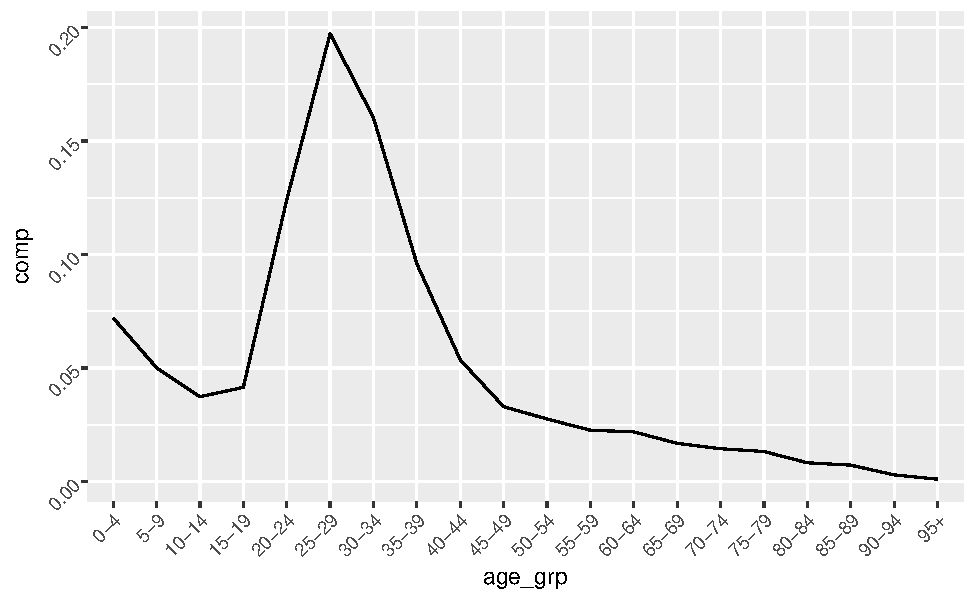
\includegraphics{_main_files/figure-latex/unnamed-chunk-118-1.pdf}

\hypertarget{log-linear-models}{%
\section{Log-Linear Models}\label{log-linear-models}}

\hypertarget{log-linear-models-1}{%
\subsection{Log-Linear Models}\label{log-linear-models-1}}

\begin{itemize}
\tightlist
\item
  Rogers' and collaborators like to shorten the multiplicative form of the log-linear model to use capital letters to represent parameters
  \[
  m_{ij} = \gamma \alpha_i \beta_j \delta_{ij} = T O_i D_j OD_{ij}
  \]
\item
  When there is multiple origin-destination tables, by different age groups, sex, education level, etc,\ldots{} the notation can be easily used to study different log-linear models
  \[
  m_{ij} = T O_i D_j A_x OD_{ij} OA_{ix}
  \]
\item
  When data is in a tidy format with row \(h\) would be:
  \[
  \begin{aligned}
  \log y_{h} =&  \beta_0 +  \beta_1 ORIG_{h} + \beta_2 DEST_{h} + \beta_3 AGE_{x} + \\
  &\beta_4 ORIG_{h}:DEST_{h} + \beta_5 ORIG_{h}:AGE_{h} 
  \end{aligned}
  \]
\end{itemize}

\hypertarget{log-linear-models-2}{%
\subsection{Log-Linear Models}\label{log-linear-models-2}}

\begin{itemize}
\tightlist
\item
  We can fit log-linear models in R using the \texttt{glm()} function (for generalised linear models)
\item
  Requires a \texttt{formula}, \texttt{data} and \texttt{family} argument
\item
  The \texttt{formula} argument is similar to that in \texttt{xtabs()}, where we use the \texttt{\textasciitilde{}} symbol to separate the the response and explanatory variables

  \begin{itemize}
  \tightlist
  \item
    For example the model in the previous slide would use \texttt{formula\ =\ flow\ \textasciitilde{}\ orig\ +\ dest\ +\ age\ +\ orig:dest\ +\ orig:age}
  \item
    Use \texttt{:} or \texttt{*} to denote interactions
  \end{itemize}
\item
  The \texttt{family} argument should be set to \texttt{poisson()} for a log-linear model
\end{itemize}

\hypertarget{log-linear-models-3}{%
\subsection{Log-Linear Models}\label{log-linear-models-3}}

\begin{itemize}
\tightlist
\item
  Example with age-specific migration flows between Italian regions in 1970
\end{itemize}

\begin{Shaded}
\begin{Highlighting}[]
\NormalTok{d1 }\OtherTok{\textless{}{-}}\NormalTok{ italy\_area }\SpecialCharTok{\%\textgreater{}\%}
  \FunctionTok{filter}\NormalTok{(orig }\SpecialCharTok{!=}\NormalTok{ dest, }
\NormalTok{         year }\SpecialCharTok{==} \DecValTok{1970}\NormalTok{) }\SpecialCharTok{\%\textgreater{}\%}
  \CommentTok{\# rename so later output fits on slide}
  \FunctionTok{rename}\NormalTok{(}\AttributeTok{age =}\NormalTok{ age\_grp)}
\NormalTok{d1}
\end{Highlighting}
\end{Shaded}

\begin{verbatim}
## # A tibble: 400 x 5
##    orig       dest        year age    flow
##    <chr>      <chr>      <dbl> <fct> <dbl>
##  1 North-East North-West  1970 0-4    2350
##  2 Center     North-West  1970 0-4    1687
##  3 South      North-West  1970 0-4    9697
##  4 Islands    North-West  1970 0-4    5139
##  5 North-West North-East  1970 0-4    2448
##  6 Center     North-East  1970 0-4    1063
##  7 South      North-East  1970 0-4    1560
##  8 Islands    North-East  1970 0-4     689
##  9 North-West Center      1970 0-4    2097
## 10 North-East Center      1970 0-4    1183
## # ... with 390 more rows
\end{verbatim}

\hypertarget{log-linear-models-4}{%
\subsection{Log-Linear Models}\label{log-linear-models-4}}

\begin{Shaded}
\begin{Highlighting}[]
\FunctionTok{glm}\NormalTok{(}\AttributeTok{formula =}\NormalTok{ flow }\SpecialCharTok{\textasciitilde{}}\NormalTok{ orig }\SpecialCharTok{+}\NormalTok{ dest, }\AttributeTok{family =} \FunctionTok{poisson}\NormalTok{(), }\AttributeTok{data =}\NormalTok{ d1)}
\end{Highlighting}
\end{Shaded}

\begin{verbatim}
## 
## Call:  glm(formula = flow ~ orig + dest, family = poisson(), data = d1)
## 
## Coefficients:
##    (Intercept)     origIslands  origNorth-East  origNorth-West       origSouth  
##        6.39791         0.17515        -0.20852         0.99427         0.98847  
##    destIslands  destNorth-East  destNorth-West       destSouth  
##       -0.76940        -0.32536         1.08367         0.02188  
## 
## Degrees of Freedom: 399 Total (i.e. Null);  391 Residual
## Null Deviance:       758100 
## Residual Deviance: 5e+05     AIC: 503100
\end{verbatim}

\hypertarget{dimensions}{%
\section{Dimensions}\label{dimensions}}

\hypertarget{log-linear-model-analysis}{%
\subsection{Log-Linear Model Analysis}\label{log-linear-model-analysis}}

\begin{itemize}
\tightlist
\item
  As we increase the number of dimensions of the data, it might become important to understand which dimensions of the data are most important
\item
  We can use log-linear models with detailled migration data to

  \begin{itemize}
  \tightlist
  \item
    Understand the dominate dimensions, for example \citet{VanImhoff1997} \citet{rogers2002dms}
  \item
    Predict origin-destination flows with partial data, for example \citet{deBeer2010} \citet{Rogers2003a} \citet{Raymer2007b}
  \item
    Project detailed origin-destination flows, for example \citet{Raymer2006}
  \end{itemize}
\item
  All the above examples involve fitting a number log-linear models based on different dimensions of the data frames

  \begin{itemize}
  \tightlist
  \item
    Use model fit statistics to judge the best model
  \end{itemize}
\end{itemize}

\hypertarget{log-linear-model-analysis-1}{%
\subsection{Log-Linear Model Analysis}\label{log-linear-model-analysis-1}}

\begin{itemize}
\tightlist
\item
  One approach to choosing the most important dimensions is to fit all possible combinations of models - known as \emph{dredging} the model space
\item
  The \texttt{dredge()} function in the \emph{MuMIn} package will fit all combinations of regression models given an upper limit, i.e.~the most complex model.

  \begin{itemize}
  \tightlist
  \item
    The number of combinations grows exponentially with the number of predictors
  \item
    Does not allow \texttt{na.action\ =\ "na.omit"} - set by default in \texttt{glm()} for handling missing values in regression models
  \end{itemize}
\end{itemize}

\hypertarget{log-linear-model-analysis-2}{%
\subsection{Log-Linear Model Analysis}\label{log-linear-model-analysis-2}}

\begin{itemize}
\tightlist
\item
  Fit the most complex model using \texttt{glm()}.

  \begin{itemize}
  \tightlist
  \item
    Set \texttt{na.action\ =\ na.fail} to exclude failed models in when using the \texttt{dredge()} function later
  \item
    Most complex model typically involves at least all two-way interactions
  \end{itemize}
\item
  The \texttt{formula} argument in \texttt{glm()} allows the use \texttt{()\^{}2} to construct all two-way interactions, i.e.~the below give the identical outputs

  \begin{itemize}
  \tightlist
  \item
    Use \texttt{()\^{}3} for all three way interactions
  \end{itemize}
\end{itemize}

\begin{Shaded}
\begin{Highlighting}[]
\NormalTok{f1 }\OtherTok{\textless{}{-}} \FunctionTok{glm}\NormalTok{(}\AttributeTok{formula =}\NormalTok{ flow }\SpecialCharTok{\textasciitilde{}}\NormalTok{ (orig }\SpecialCharTok{+}\NormalTok{ dest }\SpecialCharTok{+}\NormalTok{ age)}\SpecialCharTok{\^{}}\DecValTok{2}\NormalTok{, }
          \AttributeTok{family =} \FunctionTok{poisson}\NormalTok{(), }\AttributeTok{data =}\NormalTok{ d1, }\AttributeTok{na.action =}\NormalTok{ na.fail)}
\NormalTok{f2 }\OtherTok{\textless{}{-}} \FunctionTok{glm}\NormalTok{(}\AttributeTok{formula =}\NormalTok{ flow }\SpecialCharTok{\textasciitilde{}}\NormalTok{ orig }\SpecialCharTok{*}\NormalTok{ dest }\SpecialCharTok{+}\NormalTok{ orig }\SpecialCharTok{*}\NormalTok{ age }\SpecialCharTok{+}\NormalTok{ dest }\SpecialCharTok{*}\NormalTok{ age,}
          \AttributeTok{family =} \FunctionTok{poisson}\NormalTok{(), }\AttributeTok{data =}\NormalTok{ d1, }\AttributeTok{na.action =}\NormalTok{ na.fail)}

\CommentTok{\# check terms used in models}
\FunctionTok{attr}\NormalTok{(f1}\SpecialCharTok{$}\NormalTok{terms, }\StringTok{"term.labels"}\NormalTok{)}
\end{Highlighting}
\end{Shaded}

\begin{verbatim}
## [1] "orig"      "dest"      "age"       "orig:dest" "orig:age"  "dest:age"
\end{verbatim}

\begin{Shaded}
\begin{Highlighting}[]
\FunctionTok{attr}\NormalTok{(f2}\SpecialCharTok{$}\NormalTok{terms, }\StringTok{"term.labels"}\NormalTok{)}
\end{Highlighting}
\end{Shaded}

\begin{verbatim}
## [1] "orig"      "dest"      "age"       "orig:dest" "orig:age"  "dest:age"
\end{verbatim}

\hypertarget{log-linear-model-analysis-3}{%
\subsection{Log-Linear Model Analysis}\label{log-linear-model-analysis-3}}

\begin{itemize}
\tightlist
\item
  Models will have many estimated coefficients

  \begin{itemize}
  \tightlist
  \item
    Some will be non-determinable because no observations (e.g.~diagonal terms such as \texttt{origIslands:destIslands} below) as
  \end{itemize}
\end{itemize}

\begin{Shaded}
\begin{Highlighting}[]
\NormalTok{f1 }\SpecialCharTok{\%\textgreater{}\%} 
  \FunctionTok{coef}\NormalTok{() }\SpecialCharTok{\%\textgreater{}\%} 
  \FunctionTok{length}\NormalTok{()}
\end{Highlighting}
\end{Shaded}

\begin{verbatim}
## [1] 196
\end{verbatim}

\begin{Shaded}
\begin{Highlighting}[]
\FunctionTok{summary}\NormalTok{(f1)}
\end{Highlighting}
\end{Shaded}

\begin{verbatim}
## 
## Call:
## glm(formula = flow ~ (orig + dest + age)^2, family = poisson(), 
##     data = d1, na.action = na.fail)
## 
## Deviance Residuals: 
##      Min        1Q    Median        3Q       Max  
## -12.1125   -1.4474    0.0186    1.5870    8.3143  
## 
## Coefficients: (5 not defined because of singularities)
##                                 Estimate Std. Error z value Pr(>|z|)    
## (Intercept)                    6.812e+00  2.085e-02 326.747  < 2e-16 ***
## origIslands                    4.277e-01  2.236e-02  19.126  < 2e-16 ***
## origNorth-East                 1.709e-01  2.390e-02   7.151 8.64e-13 ***
## origNorth-West                 7.906e-01  1.789e-02  44.190  < 2e-16 ***
## origSouth                      1.381e+00  2.027e-02  68.123  < 2e-16 ***
## destIslands                   -1.548e-01  2.457e-02  -6.301 2.95e-10 ***
## destNorth-East                 8.107e-02  2.232e-02   3.632 0.000281 ***
## destNorth-West                 6.751e-01  1.856e-02  36.367  < 2e-16 ***
## destSouth                      8.315e-01  1.833e-02  45.350  < 2e-16 ***
## age5-9                        -1.073e-01  2.726e-02  -3.935 8.32e-05 ***
## age10-14                      -5.531e-01  3.071e-02 -18.012  < 2e-16 ***
## age15-19                      -6.345e-01  2.921e-02 -21.725  < 2e-16 ***
## age20-24                       5.581e-01  2.340e-02  23.850  < 2e-16 ***
## age25-29                       6.591e-01  2.378e-02  27.715  < 2e-16 ***
## age30-34                       4.155e-01  2.550e-02  16.296  < 2e-16 ***
## age35-39                       3.452e-02  2.846e-02   1.213 0.225246    
## age40-44                      -2.132e-01  3.082e-02  -6.916 4.65e-12 ***
## age45-49                      -4.331e-01  3.333e-02 -12.995  < 2e-16 ***
## age50-54                      -8.007e-01  3.911e-02 -20.475  < 2e-16 ***
## age55-59                      -7.723e-01  3.884e-02 -19.884  < 2e-16 ***
## age60-64                      -8.835e-01  4.067e-02 -21.721  < 2e-16 ***
## age65-69                      -1.017e+00  4.508e-02 -22.565  < 2e-16 ***
## age70-74                      -1.284e+00  5.087e-02 -25.242  < 2e-16 ***
## age75-79                      -1.602e+00  6.015e-02 -26.628  < 2e-16 ***
## age80-84                      -2.099e+00  7.796e-02 -26.932  < 2e-16 ***
## age85-89                      -2.798e+00  1.164e-01 -24.039  < 2e-16 ***
## age90-94                      -4.022e+00  2.183e-01 -18.422  < 2e-16 ***
## age95+                        -3.872e+00  1.344e-01 -28.816  < 2e-16 ***
## origIslands:destIslands               NA         NA      NA       NA    
## origNorth-East:destIslands    -7.535e-01  2.394e-02 -31.472  < 2e-16 ***
## origNorth-West:destIslands     4.133e-01  1.590e-02  25.998  < 2e-16 ***
## origSouth:destIslands         -1.450e+00  2.079e-02 -69.771  < 2e-16 ***
## origIslands:destNorth-East    -8.276e-01  2.016e-02 -41.062  < 2e-16 ***
## origNorth-East:destNorth-East         NA         NA      NA       NA    
## origNorth-West:destNorth-East  1.723e-01  1.388e-02  12.414  < 2e-16 ***
## origSouth:destNorth-East      -9.378e-01  1.701e-02 -55.130  < 2e-16 ***
## origIslands:destNorth-West     6.005e-01  1.622e-02  37.030  < 2e-16 ***
## origNorth-East:destNorth-West  1.862e-01  1.703e-02  10.934  < 2e-16 ***
## origNorth-West:destNorth-West         NA         NA      NA       NA    
## origSouth:destNorth-West       2.968e-01  1.460e-02  20.336  < 2e-16 ***
## origIslands:destSouth         -1.346e+00  1.700e-02 -79.141  < 2e-16 ***
## origNorth-East:destSouth      -1.000e+00  1.672e-02 -59.838  < 2e-16 ***
## origNorth-West:destSouth              NA         NA      NA       NA    
## origSouth:destSouth                   NA         NA      NA       NA    
## origIslands:age5-9             3.728e-02  2.705e-02   1.379 0.168013    
## origNorth-East:age5-9         -3.398e-02  2.976e-02  -1.142 0.253461    
## origNorth-West:age5-9         -2.097e-02  2.469e-02  -0.849 0.395888    
## origSouth:age5-9               6.147e-02  2.489e-02   2.470 0.013522 *  
## origIslands:age10-14           2.034e-01  3.009e-02   6.759 1.39e-11 ***
## origNorth-East:age10-14       -8.982e-02  3.415e-02  -2.630 0.008533 ** 
## origNorth-West:age10-14       -3.405e-02  2.853e-02  -1.193 0.232730    
## origSouth:age10-14             2.270e-01  2.788e-02   8.145 3.81e-16 ***
## origIslands:age15-19           4.832e-01  2.807e-02  17.213  < 2e-16 ***
## origNorth-East:age15-19       -1.154e-01  3.267e-02  -3.533 0.000410 ***
## origNorth-West:age15-19       -3.695e-02  2.712e-02  -1.363 0.173004    
## origSouth:age15-19             5.775e-01  2.617e-02  22.066  < 2e-16 ***
## origIslands:age20-24           6.953e-02  2.297e-02   3.027 0.002470 ** 
## origNorth-East:age20-24       -7.223e-02  2.531e-02  -2.853 0.004327 ** 
## origNorth-West:age20-24       -3.782e-01  2.141e-02 -17.664  < 2e-16 ***
## origSouth:age20-24             1.541e-01  2.112e-02   7.296 2.96e-13 ***
## origIslands:age25-29          -2.259e-01  2.368e-02  -9.536  < 2e-16 ***
## origNorth-East:age25-29       -4.052e-02  2.548e-02  -1.590 0.111742    
## origNorth-West:age25-29       -3.300e-01  2.148e-02 -15.358  < 2e-16 ***
## origSouth:age25-29            -2.484e-01  2.170e-02 -11.445  < 2e-16 ***
## origIslands:age30-34          -3.437e-01  2.586e-02 -13.293  < 2e-16 ***
## origNorth-East:age30-34       -1.532e-02  2.737e-02  -0.560 0.575692    
## origNorth-West:age30-34       -2.374e-01  2.295e-02 -10.342  < 2e-16 ***
## origSouth:age30-34            -3.716e-01  2.357e-02 -15.767  < 2e-16 ***
## origIslands:age35-39          -3.622e-01  2.905e-02 -12.467  < 2e-16 ***
## origNorth-East:age35-39       -6.987e-02  3.080e-02  -2.268 0.023322 *  
## origNorth-West:age35-39       -2.315e-01  2.580e-02  -8.975  < 2e-16 ***
## origSouth:age35-39            -3.976e-01  2.642e-02 -15.053  < 2e-16 ***
## origIslands:age40-44          -3.607e-01  3.147e-02 -11.462  < 2e-16 ***
## origNorth-East:age40-44       -9.838e-02  3.354e-02  -2.933 0.003353 ** 
## origNorth-West:age40-44       -2.872e-01  2.835e-02 -10.130  < 2e-16 ***
## origSouth:age40-44            -3.450e-01  2.847e-02 -12.120  < 2e-16 ***
## origIslands:age45-49          -4.171e-01  3.414e-02 -12.215  < 2e-16 ***
## origNorth-East:age45-49       -1.373e-01  3.628e-02  -3.784 0.000155 ***
## origNorth-West:age45-49       -3.409e-01  3.073e-02 -11.093  < 2e-16 ***
## origSouth:age45-49            -3.791e-01  3.068e-02 -12.360  < 2e-16 ***
## origIslands:age50-54          -4.729e-01  4.048e-02 -11.681  < 2e-16 ***
## origNorth-East:age50-54       -1.693e-01  4.272e-02  -3.963 7.41e-05 ***
## origNorth-West:age50-54       -4.082e-01  3.613e-02 -11.299  < 2e-16 ***
## origSouth:age50-54            -4.723e-01  3.625e-02 -13.028  < 2e-16 ***
## origIslands:age55-59          -6.000e-01  4.066e-02 -14.756  < 2e-16 ***
## origNorth-East:age55-59       -1.545e-01  4.206e-02  -3.673 0.000239 ***
## origNorth-West:age55-59       -2.769e-01  3.496e-02  -7.920 2.38e-15 ***
## origSouth:age55-59            -6.989e-01  3.652e-02 -19.140  < 2e-16 ***
## origIslands:age60-64          -7.392e-01  4.388e-02 -16.847  < 2e-16 ***
## origNorth-East:age60-64       -1.382e-01  4.412e-02  -3.133 0.001731 ** 
## origNorth-West:age60-64       -1.846e-01  3.600e-02  -5.128 2.93e-07 ***
## origSouth:age60-64            -7.990e-01  3.874e-02 -20.624  < 2e-16 ***
## origIslands:age65-69          -7.861e-01  4.896e-02 -16.054  < 2e-16 ***
## origNorth-East:age65-69       -1.845e-01  4.884e-02  -3.777 0.000158 ***
## origNorth-West:age65-69       -3.790e-01  4.019e-02  -9.430  < 2e-16 ***
## origSouth:age65-69            -8.881e-01  4.337e-02 -20.475  < 2e-16 ***
## origIslands:age70-74          -7.729e-01  5.541e-02 -13.948  < 2e-16 ***
## origNorth-East:age70-74       -1.764e-01  5.511e-02  -3.200 0.001375 ** 
## origNorth-West:age70-74       -4.427e-01  4.583e-02  -9.659  < 2e-16 ***
## origSouth:age70-74            -8.297e-01  4.879e-02 -17.006  < 2e-16 ***
## origIslands:age75-79          -7.637e-01  6.539e-02 -11.680  < 2e-16 ***
## origNorth-East:age75-79       -1.946e-01  6.473e-02  -3.006 0.002648 ** 
## origNorth-West:age75-79       -6.148e-01  5.490e-02 -11.197  < 2e-16 ***
## origSouth:age75-79            -8.376e-01  5.775e-02 -14.503  < 2e-16 ***
## origIslands:age80-84          -8.643e-01  8.598e-02 -10.052  < 2e-16 ***
## origNorth-East:age80-84       -2.304e-01  8.370e-02  -2.752 0.005924 ** 
## origNorth-West:age80-84       -6.198e-01  7.212e-02  -8.594  < 2e-16 ***
## origSouth:age80-84            -9.215e-01  7.535e-02 -12.229  < 2e-16 ***
## origIslands:age85-89          -9.459e-01  1.281e-01  -7.382 1.56e-13 ***
## origNorth-East:age85-89       -3.505e-01  1.260e-01  -2.783 0.005392 ** 
## origNorth-West:age85-89       -7.537e-01  1.086e-01  -6.941 3.91e-12 ***
## origSouth:age85-89            -1.126e+00  1.145e-01  -9.832  < 2e-16 ***
## origIslands:age90-94          -7.778e-01  2.418e-01  -3.217 0.001296 ** 
## origNorth-East:age90-94       -2.249e-01  2.404e-01  -0.935 0.349581    
## origNorth-West:age90-94       -6.822e-01  2.080e-01  -3.279 0.001041 ** 
## origSouth:age90-94            -9.923e-01  2.186e-01  -4.539 5.64e-06 ***
## origIslands:age95+            -1.078e-01  1.304e-01  -0.826 0.408661    
## origNorth-East:age95+         -1.944e-01  1.469e-01  -1.324 0.185566    
## origNorth-West:age95+         -2.803e-01  1.106e-01  -2.533 0.011308 *  
## origSouth:age95+              -2.948e-01  1.218e-01  -2.420 0.015542 *  
## destIslands:age5-9            -1.202e-01  2.898e-02  -4.149 3.33e-05 ***
## destNorth-East:age5-9          1.725e-02  2.578e-02   0.669 0.503388    
## destNorth-West:age5-9          7.266e-03  1.974e-02   0.368 0.712823    
## destSouth:age5-9              -1.636e-01  2.533e-02  -6.457 1.07e-10 ***
## destIslands:age10-14          -1.703e-01  3.301e-02  -5.159 2.48e-07 ***
## destNorth-East:age10-14        1.697e-02  2.858e-02   0.594 0.552693    
## destNorth-West:age10-14        9.830e-02  2.152e-02   4.567 4.94e-06 ***
## destSouth:age10-14            -2.812e-01  2.911e-02  -9.660  < 2e-16 ***
## destIslands:age15-19           1.533e-01  3.050e-02   5.026 5.00e-07 ***
## destNorth-East:age15-19        1.060e-01  2.717e-02   3.903 9.52e-05 ***
## destNorth-West:age15-19        3.282e-01  2.014e-02  16.292  < 2e-16 ***
## destSouth:age15-19             3.606e-02  2.733e-02   1.319 0.187003    
## destIslands:age20-24           3.125e-02  2.500e-02   1.250 0.211310    
## destNorth-East:age20-24        1.057e-01  2.238e-02   4.723 2.33e-06 ***
## destNorth-West:age20-24        9.761e-02  1.695e-02   5.757 8.55e-09 ***
## destSouth:age20-24            -1.516e-01  2.221e-02  -6.828 8.63e-12 ***
## destIslands:age25-29          -1.739e-01  2.569e-02  -6.767 1.31e-11 ***
## destNorth-East:age25-29        1.137e-02  2.299e-02   0.494 0.620982    
## destNorth-West:age25-29       -8.689e-02  1.763e-02  -4.928 8.32e-07 ***
## destSouth:age25-29            -2.597e-01  2.245e-02 -11.568  < 2e-16 ***
## destIslands:age30-34          -3.411e-01  2.782e-02 -12.263  < 2e-16 ***
## destNorth-East:age30-34       -7.689e-03  2.445e-02  -0.314 0.753161    
## destNorth-West:age30-34       -2.411e-01  1.911e-02 -12.617  < 2e-16 ***
## destSouth:age30-34            -3.476e-01  2.397e-02 -14.500  < 2e-16 ***
## destIslands:age35-39          -4.423e-01  3.165e-02 -13.973  < 2e-16 ***
## destNorth-East:age35-39       -1.997e-02  2.713e-02  -0.736 0.461614    
## destNorth-West:age35-39       -2.643e-01  2.137e-02 -12.367  < 2e-16 ***
## destSouth:age35-39            -4.538e-01  2.710e-02 -16.746  < 2e-16 ***
## destIslands:age40-44          -5.245e-01  3.517e-02 -14.913  < 2e-16 ***
## destNorth-East:age40-44       -1.014e-02  2.922e-02  -0.347 0.728693    
## destNorth-West:age40-44       -2.404e-01  2.293e-02 -10.483  < 2e-16 ***
## destSouth:age40-44            -5.495e-01  3.000e-02 -18.315  < 2e-16 ***
## destIslands:age45-49          -4.948e-01  3.830e-02 -12.919  < 2e-16 ***
## destNorth-East:age45-49        9.649e-03  3.171e-02   0.304 0.760938    
## destNorth-West:age45-49       -2.253e-01  2.498e-02  -9.021  < 2e-16 ***
## destSouth:age45-49            -5.734e-01  3.300e-02 -17.373  < 2e-16 ***
## destIslands:age50-54          -4.942e-01  4.522e-02 -10.927  < 2e-16 ***
## destNorth-East:age50-54        4.565e-06  3.725e-02   0.000 0.999902    
## destNorth-West:age50-54       -3.163e-01  2.972e-02 -10.640  < 2e-16 ***
## destSouth:age50-54            -6.328e-01  3.937e-02 -16.074  < 2e-16 ***
## destIslands:age55-59          -5.805e-01  4.541e-02 -12.783  < 2e-16 ***
## destNorth-East:age55-59        9.658e-02  3.664e-02   2.636 0.008385 ** 
## destNorth-West:age55-59       -2.985e-01  3.060e-02  -9.756  < 2e-16 ***
## destSouth:age55-59            -6.443e-01  3.864e-02 -16.674  < 2e-16 ***
## destIslands:age60-64          -6.453e-01  4.780e-02 -13.500  < 2e-16 ***
## destNorth-East:age60-64        1.870e-01  3.768e-02   4.962 6.99e-07 ***
## destNorth-West:age60-64       -3.416e-01  3.289e-02 -10.386  < 2e-16 ***
## destSouth:age60-64            -6.588e-01  4.018e-02 -16.396  < 2e-16 ***
## destIslands:age65-69          -6.577e-01  5.361e-02 -12.268  < 2e-16 ***
## destNorth-East:age65-69        8.760e-02  4.258e-02   2.057 0.039641 *  
## destNorth-West:age65-69       -4.820e-01  3.682e-02 -13.092  < 2e-16 ***
## destSouth:age65-69            -7.019e-01  4.519e-02 -15.533  < 2e-16 ***
## destIslands:age70-74          -7.064e-01  6.179e-02 -11.431  < 2e-16 ***
## destNorth-East:age70-74        5.675e-02  4.816e-02   1.178 0.238672    
## destNorth-West:age70-74       -5.134e-01  4.125e-02 -12.447  < 2e-16 ***
## destSouth:age70-74            -7.024e-01  5.130e-02 -13.692  < 2e-16 ***
## destIslands:age75-79          -6.143e-01  7.225e-02  -8.503  < 2e-16 ***
## destNorth-East:age75-79       -2.785e-02  5.832e-02  -0.477 0.633038    
## destNorth-West:age75-79       -5.902e-01  4.883e-02 -12.085  < 2e-16 ***
## destSouth:age75-79            -6.906e-01  6.135e-02 -11.257  < 2e-16 ***
## destIslands:age80-84          -7.780e-01  9.764e-02  -7.968 1.61e-15 ***
## destNorth-East:age80-84       -1.356e-01  7.696e-02  -1.762 0.078011 .  
## destNorth-West:age80-84       -5.625e-01  6.335e-02  -8.879  < 2e-16 ***
## destSouth:age80-84            -7.880e-01  8.063e-02  -9.773  < 2e-16 ***
## destIslands:age85-89          -9.642e-01  1.550e-01  -6.222 4.89e-10 ***
## destNorth-East:age85-89       -1.953e-01  1.167e-01  -1.674 0.094131 .  
## destNorth-West:age85-89       -6.426e-01  9.674e-02  -6.642 3.09e-11 ***
## destSouth:age85-89            -8.860e-01  1.227e-01  -7.220 5.20e-13 ***
## destIslands:age90-94          -1.047e+00  2.834e-01  -3.696 0.000219 ***
## destNorth-East:age90-94       -2.522e-01  2.087e-01  -1.209 0.226824    
## destNorth-West:age90-94       -8.760e-01  1.758e-01  -4.982 6.29e-07 ***
## destSouth:age90-94            -1.128e+00  2.330e-01  -4.843 1.28e-06 ***
## destIslands:age95+             2.274e-01  1.434e-01   1.586 0.112675    
## destNorth-East:age95+          4.667e-01  1.248e-01   3.740 0.000184 ***
## destNorth-West:age95+         -2.613e-01  1.108e-01  -2.359 0.018329 *  
## destSouth:age95+               2.250e-01  1.262e-01   1.783 0.074616 .  
## ---
## Signif. codes:  0 '***' 0.001 '**' 0.01 '*' 0.05 '.' 0.1 ' ' 1
## 
## (Dispersion parameter for poisson family taken to be 1)
## 
##     Null deviance: 758059.9  on 399  degrees of freedom
## Residual deviance:   2767.8  on 209  degrees of freedom
## AIC: 6272
## 
## Number of Fisher Scoring iterations: 4
\end{verbatim}

\hypertarget{log-linear-model-analysis-4}{%
\subsection{Log-Linear Model Analysis}\label{log-linear-model-analysis-4}}

\begin{itemize}
\tightlist
\item
  Pass the upper model to \texttt{dredge()}. Use \texttt{trace\ =\ TRUE} to monitor progress.
\end{itemize}

\begin{Shaded}
\begin{Highlighting}[]
\FunctionTok{library}\NormalTok{(MuMIn)}
\NormalTok{mm }\OtherTok{\textless{}{-}} \FunctionTok{dredge}\NormalTok{(}\AttributeTok{global.model =}\NormalTok{ f1, }\AttributeTok{trace =} \ConstantTok{TRUE}\NormalTok{)}
\end{Highlighting}
\end{Shaded}

\begin{verbatim}
## Fixed term is "(Intercept)"
\end{verbatim}

\begin{verbatim}
## 0 : glm(formula = flow ~ 1, family = poisson(), data = d1, na.action = na.fail)
## 1 : glm(formula = flow ~ age + 1, family = poisson(), data = d1, 
##     na.action = na.fail)
## 2 : glm(formula = flow ~ dest + 1, family = poisson(), data = d1, 
##     na.action = na.fail)
## 3 : glm(formula = flow ~ age + dest + 1, family = poisson(), data = d1, 
##     na.action = na.fail)
## 4 : glm(formula = flow ~ orig + 1, family = poisson(), data = d1, 
##     na.action = na.fail)
## 5 : glm(formula = flow ~ age + orig + 1, family = poisson(), data = d1, 
##     na.action = na.fail)
## 6 : glm(formula = flow ~ dest + orig + 1, family = poisson(), data = d1, 
##     na.action = na.fail)
## 7 : glm(formula = flow ~ age + dest + orig + 1, family = poisson(), 
##     data = d1, na.action = na.fail)
## 11 : glm(formula = flow ~ age + dest + age:dest + 1, family = poisson(), 
##     data = d1, na.action = na.fail)
## 15 : glm(formula = flow ~ age + dest + orig + age:dest + 1, family = poisson(), 
##     data = d1, na.action = na.fail)
## 21 : glm(formula = flow ~ age + orig + age:orig + 1, family = poisson(), 
##     data = d1, na.action = na.fail)
## 23 : glm(formula = flow ~ age + dest + orig + age:orig + 1, family = poisson(), 
##     data = d1, na.action = na.fail)
## 31 : glm(formula = flow ~ age + dest + orig + age:dest + age:orig + 
##     1, family = poisson(), data = d1, na.action = na.fail)
## 38 : glm(formula = flow ~ dest + orig + dest:orig + 1, family = poisson(), 
##     data = d1, na.action = na.fail)
## 39 : glm(formula = flow ~ age + dest + orig + dest:orig + 1, family = poisson(), 
##     data = d1, na.action = na.fail)
## 47 : glm(formula = flow ~ age + dest + orig + age:dest + dest:orig + 
##     1, family = poisson(), data = d1, na.action = na.fail)
## 55 : glm(formula = flow ~ age + dest + orig + age:orig + dest:orig + 
##     1, family = poisson(), data = d1, na.action = na.fail)
## 63 : glm(formula = flow ~ age + dest + orig + age:dest + age:orig + 
##     dest:orig + 1, family = poisson(), data = d1, na.action = na.fail)
\end{verbatim}

\hypertarget{log-linear-model-analysis-5}{%
\subsection{Log-Linear Model Analysis}\label{log-linear-model-analysis-5}}

\begin{Shaded}
\begin{Highlighting}[]
\NormalTok{mm}
\end{Highlighting}
\end{Shaded}

\begin{verbatim}
## Global model call: glm(formula = flow ~ (orig + dest + age)^2, family = poisson(), 
##     data = d1, na.action = na.fail)
## ---
## Model selection table 
##    (Int) age dst org age:dst age:org dst:org  df      logLik     AICc     delta
## 64 6.515   +   +   +       +       +       + 191   -2944.992   6624.6      0.00
## 56 6.616   +   +   +               +       + 115   -5286.311  10896.6   4271.97
## 48 6.619   +   +   +       +               + 115   -7617.005  15558.0   8933.35
## 40 6.691   +   +   +                       +  39  -11408.460  22903.6  16278.99
## 32 6.865   +   +   +       +       +         180  -22817.598  46292.7  39668.13
## 24 6.995   +   +   +               +         104  -25545.324  51372.7  44748.08
## 16 6.997   +   +   +       +                 104  -27876.018  56034.1  49409.47
## 8  7.070   +   +   +                          28  -31667.473  63395.3  56770.72
## 12 7.612   +   +           +                 100  -82409.496 165086.5 158461.95
## 4  7.684   +   +                              24  -86200.951 172453.1 165828.50
## 22 7.250   +       +               +         100 -114058.016 228383.6 221758.99
## 6  7.325   +       +                          24 -120180.165 240411.5 233786.93
## 2  7.734   +                                  20 -160715.461 321473.1 314848.54
## 39 6.019       +   +                       +  20 -231284.060 462610.3 455985.74
## 7  6.398       +   +                           9 -251543.073 503104.6 496480.01
## 3  7.012       +                               5 -306076.551 612163.3 605538.65
## 5  6.653           +                           5 -340055.765 680121.7 673497.08
## 1  7.062                                       1 -380591.061 761184.1 754559.53
##    weight
## 64      1
## 56      0
## 48      0
## 40      0
## 32      0
## 24      0
## 16      0
## 8       0
## 12      0
## 4       0
## 22      0
## 6       0
## 2       0
## 39      0
## 7       0
## 3       0
## 5       0
## 1       0
## Models ranked by AICc(x)
\end{verbatim}

\hypertarget{log-linear-model-analysis-6}{%
\subsection{Log-Linear Model Analysis}\label{log-linear-model-analysis-6}}

\begin{itemize}
\tightlist
\item
  Model comparison based on model statistics measuring the goodness of fit.

  \begin{itemize}
  \tightlist
  \item
    AIC measures a goodness of fit with a penalty for the number of predictor variables.
  \item
    AICc has a bias correction term for small samples
  \end{itemize}
\item
  Typically the origin-destination interaction term is very important for accurately predicting the age-specific origin-destination migration flows
\item
  The time to conduct a dredging analysis increase exponentially as the number of dimensions increases.
\end{itemize}

\hypertarget{exercise-ex6.r}{%
\subsection{Exercise (ex6.R)}\label{exercise-ex6.r}}

\begin{Shaded}
\begin{Highlighting}[]
\CommentTok{\# 0.  a) Load the KOSTAT2021.Rproj file. }
\CommentTok{\#     Run the getwd() below. It should print the directory where the }
\CommentTok{\#     KOSTAT2021.Rproj file is located.}
\FunctionTok{getwd}\NormalTok{()}
\CommentTok{\#     b) Load the packages used in this exercise}
\FunctionTok{library}\NormalTok{(tidyverse)}
\FunctionTok{library}\NormalTok{(migest)}
\FunctionTok{library}\NormalTok{(MuMIn)}
\DocumentationTok{\#\#}
\DocumentationTok{\#\#}
\DocumentationTok{\#\#}
\CommentTok{\# 1. Run the code below to read in the migration flow data for flows within the }
\CommentTok{\#    USA, decomposed by move type, from 6 censuses between 1940 and 2000. }
\NormalTok{us }\OtherTok{\textless{}{-}} \FunctionTok{read\_csv}\NormalTok{(}\StringTok{"./data/us\_area\_1940\_2000.csv"}\NormalTok{)}
\NormalTok{us}
\CommentTok{\# 2. Show the multiplicative components, rounded to 3 digits, for the flows from}
\CommentTok{\#    the 2000 census}
\NormalTok{us }\SpecialCharTok{\%\textgreater{}\%}
  \FunctionTok{filter}\NormalTok{(year }\SpecialCharTok{==} \DecValTok{2000}\NormalTok{) }\SpecialCharTok{\%\textgreater{}\%}
  \DocumentationTok{\#\#\#\#\#() \%\textgreater{}\%}
  \FunctionTok{round}\NormalTok{(}\AttributeTok{digits =} \DocumentationTok{\#\#\#\#\#)}
\CommentTok{\# 3. Fit a log{-}linear model to the entire data set using all two{-}way }
\CommentTok{\#    interactions between the four dimensions (orig, dest, period and move\_type)}
\NormalTok{f }\OtherTok{\textless{}{-}} \FunctionTok{glm}\NormalTok{(}\AttributeTok{formula =}\NormalTok{ flow }\SpecialCharTok{\textasciitilde{}}\NormalTok{ (}\DocumentationTok{\#\#\#\#\# + dest + \#\#\#\#\# + move\_type) \^{}\#\#\#\#\#,}
         \AttributeTok{family =} \DocumentationTok{\#\#\#\#\#(), data = us, na.action = na.fail)}
\CommentTok{\# 4. View a summary of the model }
\FunctionTok{summary}\NormalTok{(}\DocumentationTok{\#\#\#\#\#)}
\CommentTok{\# 5. Use dredge() to fit all simpler models than the model saved in f}
\NormalTok{mm }\OtherTok{\textless{}{-}} \DocumentationTok{\#\#\#\#\#(global.model = f, trace = TRUE)}
\CommentTok{\# 6. Use the View() function to inspect the results of the dredging of the model }
\CommentTok{\#    space and identify the most important dimensions}
\FunctionTok{View}\NormalTok{(mm)}
\end{Highlighting}
\end{Shaded}

\hypertarget{estimating-bilateral-migration}{%
\chapter{Estimating Bilateral Migration}\label{estimating-bilateral-migration}}

\hypertarget{ipfp}{%
\section{IPFP}\label{ipfp}}

\hypertarget{ipfp-1}{%
\subsection{IPFP}\label{ipfp-1}}

\begin{itemize}
\tightlist
\item
  A common problem with bilateral migration data is that it is unavailable or outdated.

  \begin{itemize}
  \tightlist
  \item
    Often collected in censuses
  \end{itemize}
\item
  In some cases there are other data sources available that provide information on the in- and out-migration totals

  \begin{itemize}
  \tightlist
  \item
    Population registers
  \end{itemize}
\end{itemize}

\emph{Origin}

\emph{Destination}

\emph{Origin}

\emph{Destination}

A

B

C

D

Sum

A

B

C

D

Sum

A

100

30

70

200

A

250

B

50

45

5

100

B

75

C

60

35

40

135

C

125

D

20

25

20

65

D

150

Sum

130

160

95

115

500

Sum

150

200

50

200

600

\hypertarget{ipfp-2}{%
\subsection{IPFP}\label{ipfp-2}}

\begin{itemize}
\tightlist
\item
  This provides a data estimation challenge, where the marginal tables totals are known but the cell values are known.
\item
  Similar data estimation challenges exist for more detailed migration flow tables, for example:

  \begin{itemize}
  \tightlist
  \item
    In- and out-migration totals by age in each region are known, but the origin-destination migration flow table for each age group is missing.
  \item
    Required by multi-regional cohort-component models
  \item
    Estimating international migration flows from stocks (see for example \citet{Abel2013} )
  \end{itemize}
\end{itemize}

\hypertarget{ipfp-3}{%
\subsection{IPFP}\label{ipfp-3}}

\begin{itemize}
\tightlist
\item
  A popular approach to estimate values in a contingency table based on known marginal tables and an initial contingency table is the Iterative Proportional Fitting Procedure (IPFP).
\item
  First described by \citet{Deming1940}, the IPFP has since been widely studied in a number of different disciplines and under a number of synonyms such as raking, matrix scaling or the RAS algorithm

  \begin{itemize}
  \tightlist
  \item
    \citet{Lovelace2015} gives a good overview of the application of IPFP in social sciences.
  \item
    \citet{Lomax2016} for another overview more specific to demography.
  \end{itemize}
\item
  Mathematical approach to iteratively adjust a \emph{seed} contingency table \(\mu_{ij}^{(0)} = m_{ij}\) to known row and column totals (\(n_{i+}\) and \(n_{+j}\))
  \[
  \mu_{ij}^{(t+1)} = \frac{\mu_{ij}^{(t)}}{\mu_{i+}^{(t)}}n_{i+} \qquad \mu_{ij}^{(t+2)} = \frac{\mu_{ij}^{(t+1)}}{\mu_{+j}^{(t+1)}}n_{+j}
  \]
\end{itemize}

\hypertarget{ipfp-4}{%
\subsection{IPFP}\label{ipfp-4}}

\emph{Origin}

\emph{Destination}

\emph{Origin}

\emph{Destination}

A

B

C

D

Sum

A

B

C

D

Sum

A

100

30

70

200

A

102.87

11.67

135.46

250

B

50

45

5

100

B

49.03

16.73

9.25

75

C

60

35

40

135

C

43.98

25.72

55.30

125

D

20

25

20

65

D

56.99

71.41

21.60

150

Sum

130

160

95

115

500

Sum

150

200

50

200

600

\hypertarget{ipfp-5}{%
\subsection{IPFP}\label{ipfp-5}}

\begin{itemize}
\tightlist
\item
  \citet{Willekens1999} calls the seed data an \emph{auxiliary} table and notes that it should be information on a variables related to migration.

  \begin{itemize}
  \tightlist
  \item
    Typically past migration flow data
  \item
    Distances or travel costs between the origin-destination pairs have been used where no past data exists
  \item
    Limited testing to see which seeds work best for estimating migration
  \end{itemize}
\item
  The marginal data is then known as \emph{primary} data.

  \begin{itemize}
  \tightlist
  \item
    Partial observations on the number of migrations
  \end{itemize}
\end{itemize}

\hypertarget{mipfp}{%
\subsection{mipfp}\label{mipfp}}

\begin{itemize}
\tightlist
\item
  The \emph{mipfp} package by \citet{Barthelemy2018} implements IPFP in R using the \texttt{Ipfp()} function
\item
  Can be used for multi-dimensional marginal constraint problems.
\item
  Three inputs

  \begin{itemize}
  \tightlist
  \item
    \texttt{seed} a matrix of auxiliary data to aid estimation
  \item
    \texttt{target.list} a list of dimensions that are being targeted (see next point)
  \item
    \texttt{target.data} a list of targets related to \texttt{target.list}
  \end{itemize}
\item
  R numbers dimension of arrays with

  \begin{itemize}
  \tightlist
  \item
    \texttt{1} row
  \item
    \texttt{2} column
  \item
    \texttt{3} table
  \item
    \ldots{}
  \end{itemize}
\item
  The \texttt{target.list} might involve

  \begin{itemize}
  \tightlist
  \item
    a single target, e.g.~column totals \texttt{target.list\ =\ list(2)}
  \item
    multiple targets, e.g.~row and column totals \texttt{target.list\ =\ list(1,\ 2)}
  \item
    sums over cells rather than margins of array, e.g.~cells summed over tables \texttt{target.list\ =\ list(c(1,\ 2))}
  \end{itemize}
\end{itemize}

\hypertarget{mipfp-1}{%
\subsection{mipfp}\label{mipfp-1}}

\begin{Shaded}
\begin{Highlighting}[]
\NormalTok{r }\OtherTok{\textless{}{-}}\NormalTok{ LETTERS[}\DecValTok{1}\SpecialCharTok{:}\DecValTok{4}\NormalTok{]}
\NormalTok{m0 }\OtherTok{\textless{}{-}} \FunctionTok{matrix}\NormalTok{(}\AttributeTok{data =} \FunctionTok{c}\NormalTok{(}\DecValTok{0}\NormalTok{, }\DecValTok{100}\NormalTok{, }\DecValTok{30}\NormalTok{, }\DecValTok{70}\NormalTok{, }
                      \DecValTok{50}\NormalTok{, }\DecValTok{0}\NormalTok{, }\DecValTok{45}\NormalTok{, }\DecValTok{5}\NormalTok{, }
                      \DecValTok{60}\NormalTok{, }\DecValTok{35}\NormalTok{, }\DecValTok{0}\NormalTok{, }\DecValTok{40}\NormalTok{, }
                      \DecValTok{20}\NormalTok{, }\DecValTok{25}\NormalTok{, }\DecValTok{20}\NormalTok{, }\DecValTok{0}\NormalTok{), }
             \AttributeTok{nrow =} \DecValTok{4}\NormalTok{, }\AttributeTok{ncol =} \DecValTok{4}\NormalTok{, }\AttributeTok{byrow =} \ConstantTok{TRUE}\NormalTok{, }
             \AttributeTok{dimnames =} \FunctionTok{list}\NormalTok{(}\AttributeTok{orig =}\NormalTok{ r, }\AttributeTok{dest =}\NormalTok{ r))}
\FunctionTok{addmargins}\NormalTok{(m0)}
\end{Highlighting}
\end{Shaded}

\begin{verbatim}
##      dest
## orig    A   B  C   D Sum
##   A     0 100 30  70 200
##   B    50   0 45   5 100
##   C    60  35  0  40 135
##   D    20  25 20   0  65
##   Sum 130 160 95 115 500
\end{verbatim}

\hypertarget{mipfp-2}{%
\subsection{mipfp}\label{mipfp-2}}

\begin{Shaded}
\begin{Highlighting}[]
\NormalTok{orig\_tot }\OtherTok{\textless{}{-}} \FunctionTok{c}\NormalTok{(}\DecValTok{250}\NormalTok{, }\DecValTok{75}\NormalTok{, }\DecValTok{125}\NormalTok{, }\DecValTok{150}\NormalTok{)}
\NormalTok{dest\_tot }\OtherTok{\textless{}{-}} \FunctionTok{c}\NormalTok{(}\DecValTok{150}\NormalTok{, }\DecValTok{200}\NormalTok{, }\DecValTok{50}\NormalTok{, }\DecValTok{200}\NormalTok{)}
\FunctionTok{names}\NormalTok{(orig\_tot ) }\OtherTok{\textless{}{-}} \FunctionTok{names}\NormalTok{(dest\_tot) }\OtherTok{\textless{}{-}}\NormalTok{ r}

\NormalTok{orig\_tot}
\end{Highlighting}
\end{Shaded}

\begin{verbatim}
##   A   B   C   D 
## 250  75 125 150
\end{verbatim}

\begin{Shaded}
\begin{Highlighting}[]
\NormalTok{dest\_tot}
\end{Highlighting}
\end{Shaded}

\begin{verbatim}
##   A   B   C   D 
## 150 200  50 200
\end{verbatim}

\begin{Shaded}
\begin{Highlighting}[]
\CommentTok{\# check sums are equal}
\FunctionTok{sum}\NormalTok{(orig\_tot)}
\end{Highlighting}
\end{Shaded}

\begin{verbatim}
## [1] 600
\end{verbatim}

\begin{Shaded}
\begin{Highlighting}[]
\FunctionTok{sum}\NormalTok{(dest\_tot)}
\end{Highlighting}
\end{Shaded}

\begin{verbatim}
## [1] 600
\end{verbatim}

\hypertarget{mipfp-3}{%
\subsection{mipfp}\label{mipfp-3}}

\begin{Shaded}
\begin{Highlighting}[]
\FunctionTok{library}\NormalTok{(mipfp)}
\FunctionTok{Ipfp}\NormalTok{(}\AttributeTok{seed =}\NormalTok{ m0, }\AttributeTok{target.list =} \FunctionTok{list}\NormalTok{(}\DecValTok{1}\NormalTok{, }\DecValTok{2}\NormalTok{), }
     \AttributeTok{target.data =} \FunctionTok{list}\NormalTok{(orig\_tot, dest\_tot))}
\end{Highlighting}
\end{Shaded}

\begin{verbatim}
## 
## Call:
## Ipfp(seed = m0, target.list = list(1, 2), target.data = list(orig_tot, 
##     dest_tot))
## 
## Method:  ipfp - convergence:  TRUE 
## 
## Estimates:
##     dest
## orig        A         B        C          D
##    A  0.00000 102.87046 11.67024 135.459297
##    B 49.02778   0.00000 16.72686   9.245364
##    C 43.98433  25.72033  0.00000  55.295339
##    D 56.98789  71.40921 21.60290   0.000000
\end{verbatim}

\hypertarget{mipfp-4}{%
\subsection{mipfp}\label{mipfp-4}}

\begin{Shaded}
\begin{Highlighting}[]
\CommentTok{\# save the result }
\NormalTok{y0 }\OtherTok{\textless{}{-}} \FunctionTok{Ipfp}\NormalTok{(}\AttributeTok{seed =}\NormalTok{ m0, }\AttributeTok{target.list =} \FunctionTok{list}\NormalTok{(}\DecValTok{1}\NormalTok{, }\DecValTok{2}\NormalTok{), }
           \AttributeTok{target.data =} \FunctionTok{list}\NormalTok{(orig\_tot, dest\_tot))}

\CommentTok{\# view with totals}
\FunctionTok{addmargins}\NormalTok{(y0}\SpecialCharTok{$}\NormalTok{x.hat)}
\end{Highlighting}
\end{Shaded}

\begin{verbatim}
##      dest
## orig          A         B        C          D Sum
##   A     0.00000 102.87046 11.67024 135.459297 250
##   B    49.02778   0.00000 16.72686   9.245364  75
##   C    43.98433  25.72033  0.00000  55.295339 125
##   D    56.98789  71.40921 21.60290   0.000000 150
##   Sum 150.00000 200.00000 50.00000 200.000000 600
\end{verbatim}

\hypertarget{three-dimensions}{%
\subsection{Three dimensions}\label{three-dimensions}}

Auxillary Data

\emph{Origin}

\emph{Destination}

\emph{Origin}

\emph{Destination}

A

B

C

D

Sum

A

B

C

D

Sum

A

80

10

55

145

A

20

20

15

55

B

30

20

0

50

B

20

25

5

50

C

50

15

10

75

C

10

20

30

60

D

5

20

10

35

D

15

5

10

30

Sum

85

115

40

65

305

Sum

45

45

55

50

195

Primary Data

\emph{Origin}

\emph{Destination}

A

B

C

D

Sum

A

250

B

75

C

125

D

150

Sum

150

200

50

200

600

\hypertarget{ipfp-more-complicated-data-situations}{%
\subsection{IPFP More Complicated Data Situations}\label{ipfp-more-complicated-data-situations}}

\begin{itemize}
\tightlist
\item
  The IPFP can be used for more complex data situations with more than two dimensions.
\item
  Key to using the \texttt{mipfp()} function is setting the inputs for \texttt{target.data}.
\end{itemize}

\begin{Shaded}
\begin{Highlighting}[]
\FunctionTok{library}\NormalTok{(tidyverse)}
\NormalTok{d }\OtherTok{\textless{}{-}} \FunctionTok{expand\_grid}\NormalTok{(}\AttributeTok{orig =}\NormalTok{ r, }\AttributeTok{dest =}\NormalTok{ r, }\AttributeTok{sex =} \FunctionTok{c}\NormalTok{(}\StringTok{"Female"}\NormalTok{, }\StringTok{"Male"}\NormalTok{)) }\SpecialCharTok{\%\textgreater{}\%}
  \FunctionTok{mutate}\NormalTok{(}\AttributeTok{flow =} \FunctionTok{c}\NormalTok{(}\DecValTok{0}\NormalTok{, }\DecValTok{0}\NormalTok{, }\DecValTok{80}\NormalTok{, }\DecValTok{20}\NormalTok{, }\DecValTok{10}\NormalTok{, }\DecValTok{20}\NormalTok{, }\DecValTok{55}\NormalTok{, }\DecValTok{15}\NormalTok{, }\DecValTok{30}\NormalTok{, }\DecValTok{20}\NormalTok{, }\DecValTok{0}\NormalTok{, }\DecValTok{0}\NormalTok{, }\DecValTok{20}\NormalTok{, }\DecValTok{25}\NormalTok{, }\DecValTok{0}\NormalTok{, }\DecValTok{5}\NormalTok{, }\DecValTok{50}\NormalTok{, }\DecValTok{10}\NormalTok{, }\DecValTok{15}\NormalTok{, }\DecValTok{20}\NormalTok{, }\DecValTok{0}\NormalTok{, }\DecValTok{0}\NormalTok{, }\DecValTok{10}\NormalTok{, }\DecValTok{30}\NormalTok{, }\DecValTok{5}\NormalTok{, }\DecValTok{15}\NormalTok{, }\DecValTok{20}\NormalTok{, }\DecValTok{5}\NormalTok{, }\DecValTok{10}\NormalTok{, }\DecValTok{10}\NormalTok{, }\DecValTok{0}\NormalTok{, }\DecValTok{0}\NormalTok{))}

\NormalTok{d}
\end{Highlighting}
\end{Shaded}

\begin{verbatim}
## # A tibble: 32 x 4
##    orig  dest  sex     flow
##    <chr> <chr> <chr>  <dbl>
##  1 A     A     Female     0
##  2 A     A     Male       0
##  3 A     B     Female    80
##  4 A     B     Male      20
##  5 A     C     Female    10
##  6 A     C     Male      20
##  7 A     D     Female    55
##  8 A     D     Male      15
##  9 B     A     Female    30
## 10 B     A     Male      20
## # ... with 22 more rows
\end{verbatim}

\hypertarget{estimating-detailed-bilateral-migration}{%
\subsection{Estimating Detailed Bilateral Migration}\label{estimating-detailed-bilateral-migration}}

\begin{Shaded}
\begin{Highlighting}[]
\NormalTok{m1 }\OtherTok{\textless{}{-}} \FunctionTok{xtabs}\NormalTok{(}\AttributeTok{formula =}\NormalTok{ flow }\SpecialCharTok{\textasciitilde{}}\NormalTok{ orig }\SpecialCharTok{+}\NormalTok{ dest }\SpecialCharTok{+}\NormalTok{ sex, }\AttributeTok{data =}\NormalTok{ d)}
\NormalTok{m1}
\end{Highlighting}
\end{Shaded}

\begin{verbatim}
## , , sex = Female
## 
##     dest
## orig  A  B  C  D
##    A  0 80 10 55
##    B 30  0 20  0
##    C 50 15  0 10
##    D  5 20 10  0
## 
## , , sex = Male
## 
##     dest
## orig  A  B  C  D
##    A  0 20 20 15
##    B 20  0 25  5
##    C 10 20  0 30
##    D 15  5 10  0
\end{verbatim}

\hypertarget{mipfp-5}{%
\subsection{mipfp}\label{mipfp-5}}

\begin{Shaded}
\begin{Highlighting}[]
\FunctionTok{addmargins}\NormalTok{(m1)}
\end{Highlighting}
\end{Shaded}

\begin{verbatim}
## , , sex = Female
## 
##      dest
## orig    A   B   C   D Sum
##   A     0  80  10  55 145
##   B    30   0  20   0  50
##   C    50  15   0  10  75
##   D     5  20  10   0  35
##   Sum  85 115  40  65 305
## 
## , , sex = Male
## 
##      dest
## orig    A   B   C   D Sum
##   A     0  20  20  15  55
##   B    20   0  25   5  50
##   C    10  20   0  30  60
##   D    15   5  10   0  30
##   Sum  45  45  55  50 195
## 
## , , sex = Sum
## 
##      dest
## orig    A   B   C   D Sum
##   A     0 100  30  70 200
##   B    50   0  45   5 100
##   C    60  35   0  40 135
##   D    20  25  20   0  65
##   Sum 130 160  95 115 500
\end{verbatim}

\hypertarget{mipfp-6}{%
\subsection{mipfp}\label{mipfp-6}}

\begin{Shaded}
\begin{Highlighting}[]
\FunctionTok{addmargins}\NormalTok{(m1)[,,sex }\OtherTok{=} \StringTok{"Sum"}\NormalTok{]}
\end{Highlighting}
\end{Shaded}

\begin{verbatim}
##      dest
## orig    A   B   C   D Sum
##   A     0 100  30  70 200
##   B    50   0  45   5 100
##   C    60  35   0  40 135
##   D    20  25  20   0  65
##   Sum 130 160  95 115 500
\end{verbatim}

\hypertarget{mipfp-7}{%
\subsection{mipfp}\label{mipfp-7}}

\begin{Shaded}
\begin{Highlighting}[]
\NormalTok{y1 }\OtherTok{\textless{}{-}} \FunctionTok{Ipfp}\NormalTok{(}\AttributeTok{seed =}\NormalTok{ m1, }\AttributeTok{target.list =} \FunctionTok{list}\NormalTok{(}\DecValTok{1}\NormalTok{, }\DecValTok{2}\NormalTok{), }
           \AttributeTok{target.data =} \FunctionTok{list}\NormalTok{(orig\_tot, dest\_tot))}
\FunctionTok{addmargins}\NormalTok{(y1}\SpecialCharTok{$}\NormalTok{x.hat)}
\end{Highlighting}
\end{Shaded}

\begin{verbatim}
## , , sex = Female
## 
##      dest
## orig           A          B          C          D        Sum
##   A     0.000000  82.296369   3.890080 106.432305 192.618755
##   B    29.416668   0.000000   7.434158   0.000000  36.850826
##   C    36.653611  11.022997   0.000000  13.823835  61.500444
##   D    14.246971  57.127369  10.801451   0.000000  82.175792
##   Sum  80.317251 150.446736  22.125690 120.256140 373.145817
## 
## , , sex = Male
## 
##      dest
## orig           A          B          C          D        Sum
##   A     0.000000  20.574092   7.780161  29.026992  57.381245
##   B    19.611112   0.000000   9.292698   9.245364  38.149174
##   C     7.330722  14.697330   0.000000  41.471504  63.499556
##   D    42.740914  14.281842  10.801451   0.000000  67.824208
##   Sum  69.682749  49.553264  27.874310  79.743860 226.854183
## 
## , , sex = Sum
## 
##      dest
## orig           A          B          C          D        Sum
##   A     0.000000 102.870462  11.670241 135.459297 250.000000
##   B    49.027781   0.000000  16.726856   9.245364  75.000000
##   C    43.984334  25.720327   0.000000  55.295339 125.000000
##   D    56.987886  71.409211  21.602903   0.000000 150.000000
##   Sum 150.000000 200.000000  50.000000 200.000000 600.000000
\end{verbatim}

\hypertarget{mipfp-8}{%
\subsection{mipfp}\label{mipfp-8}}

\begin{Shaded}
\begin{Highlighting}[]
\NormalTok{y1}\SpecialCharTok{$}\NormalTok{x.hat }\SpecialCharTok{\%\textgreater{}\%} 
  \FunctionTok{as.data.frame.table}\NormalTok{(}\AttributeTok{responseName =} \StringTok{"est"}\NormalTok{) }\SpecialCharTok{\%\textgreater{}\%}
  \FunctionTok{as\_tibble}\NormalTok{()}
\end{Highlighting}
\end{Shaded}

\begin{verbatim}
## # A tibble: 32 x 4
##    orig  dest  sex      est
##    <fct> <fct> <fct>  <dbl>
##  1 A     A     Female  0   
##  2 B     A     Female 29.4 
##  3 C     A     Female 36.7 
##  4 D     A     Female 14.2 
##  5 A     B     Female 82.3 
##  6 B     B     Female  0   
##  7 C     B     Female 11.0 
##  8 D     B     Female 57.1 
##  9 A     C     Female  3.89
## 10 B     C     Female  7.43
## # ... with 22 more rows
\end{verbatim}

\hypertarget{net-constraints}{%
\section{Net Constraints}\label{net-constraints}}

\hypertarget{net-constrained-origin-destination-flows}{%
\subsection{Net constrained origin-destination flows}\label{net-constrained-origin-destination-flows}}

\begin{itemize}
\tightlist
\item
  \citet{Plane1981} developed a proportional adjustment algorithm for estimating bilateral migration flows to match both

  \begin{itemize}
  \tightlist
  \item
    Constraints on the net migration of each region
  \item
    Total sum of the bilateral migration flows
  \end{itemize}
\item
  Requires knowledge of

  \begin{itemize}
  \tightlist
  \item
    Past bilateral migration flows
  \item
    Current (target) total migration flows (over whole
    system)
  \item
    Current (target) net migration flows
  \item
    Distance matrix to correspond
  \end{itemize}
\item
  No application of this method in R, although in \emph{migest} package the \texttt{cm\_net\_tot()} function provides a similar set of estimates

  \begin{itemize}
  \tightlist
  \item
    Unable to incorporate distance matrix
  \end{itemize}
\end{itemize}

\hypertarget{net-constrained-origin-destination-flows-1}{%
\subsection{Net constrained origin-destination flows}\label{net-constrained-origin-destination-flows-1}}

\begin{Shaded}
\begin{Highlighting}[]
\FunctionTok{addmargins}\NormalTok{(m0)}
\end{Highlighting}
\end{Shaded}

\begin{verbatim}
##      dest
## orig    A   B  C   D Sum
##   A     0 100 30  70 200
##   B    50   0 45   5 100
##   C    60  35  0  40 135
##   D    20  25 20   0  65
##   Sum 130 160 95 115 500
\end{verbatim}

\begin{Shaded}
\begin{Highlighting}[]
\CommentTok{\# observed net}
\FunctionTok{library}\NormalTok{(migest)}
\FunctionTok{sum\_turnover}\NormalTok{(m0)}
\end{Highlighting}
\end{Shaded}

\begin{verbatim}
## # A tibble: 4 x 5
##   region in_mig out_mig  turn   net
##   <chr>   <dbl>   <dbl> <dbl> <dbl>
## 1 A         130     200   330   -70
## 2 B         160     100   260    60
## 3 C          95     135   230   -40
## 4 D         115      65   180    50
\end{verbatim}

\hypertarget{net-constrained-origin-destination-flows-2}{%
\subsection{Net constrained origin-destination flows}\label{net-constrained-origin-destination-flows-2}}

\begin{itemize}
\tightlist
\item
  Estimate migration flows to match new net migration and grand total.
\end{itemize}

\begin{Shaded}
\begin{Highlighting}[]
\NormalTok{y1 }\OtherTok{\textless{}{-}} \FunctionTok{cm\_net\_tot}\NormalTok{(}\AttributeTok{net\_tot =} \FunctionTok{c}\NormalTok{(}\SpecialCharTok{{-}}\DecValTok{100}\NormalTok{, }\DecValTok{125}\NormalTok{, }\SpecialCharTok{{-}}\DecValTok{75}\NormalTok{, }\DecValTok{50}\NormalTok{), }\AttributeTok{tot =} \DecValTok{600}\NormalTok{, }
                 \AttributeTok{m =}\NormalTok{ m0, }\AttributeTok{verbose =} \ConstantTok{FALSE}\NormalTok{)}
\FunctionTok{addmargins}\NormalTok{(y1}\SpecialCharTok{$}\NormalTok{n)}
\end{Highlighting}
\end{Shaded}

\begin{verbatim}
##      dest
## orig          A         B        C          D       Sum
##   A     0.00000 136.22513 32.93756  79.068944 248.23163
##   B    49.88761   0.00000 42.28296   4.833488  97.00406
##   C    74.27815  50.62851  0.00000  47.977516 172.88418
##   D    24.06590  35.15032 22.66377   0.000000  81.87999
##   Sum 148.23166 222.00396 97.88429 131.879947 599.99986
\end{verbatim}

\begin{Shaded}
\begin{Highlighting}[]
\FunctionTok{sum\_turnover}\NormalTok{(y1}\SpecialCharTok{$}\NormalTok{n)}
\end{Highlighting}
\end{Shaded}

\begin{verbatim}
## # A tibble: 4 x 5
##   region in_mig out_mig  turn    net
##   <chr>   <dbl>   <dbl> <dbl>  <dbl>
## 1 A       148.    248.   396. -100. 
## 2 B       222.     97.0  319.  125. 
## 3 C        97.9   173.   271.  -75.0
## 4 D       132.     81.9  214.   50.0
\end{verbatim}

\hypertarget{net-constrained-origin-destination-flows-3}{%
\subsection{Net constrained origin-destination flows}\label{net-constrained-origin-destination-flows-3}}

\begin{itemize}
\tightlist
\item
  The requirement on the total sum of the bilateral flow for the algorithm is not realistic.
  -\citet{Plane1981} method not widely adpoted

  \begin{itemize}
  \tightlist
  \item
    In many countries the overall number of migrant flows, that is demographically consistent with natural population change, is typically not known.
  \item
    If the overall number of migrant flows is known, it is typically obtained from a comprehensive population register, and thus bilateral migration or total in- and out-migration flows already exist. If it is the later, can use IPFP approaches.
  \end{itemize}
\item
  In recent years I have been working on a method that constrains only to the net migration totals.

  \begin{itemize}
  \tightlist
  \item
    Unpublished, work in progress, use at own risk
  \item
    Method is available in the \texttt{cm\_net()} function in the \emph{migest} package
  \end{itemize}
\item
  Potential uses

  \begin{itemize}
  \tightlist
  \item
    Update bilateral migration flows from surveys or administrative data to match known demographic consistent net migration totals
  \item
    Estimate bilateral migration flows from known net migration totals using non-migration data as a seed (if no migration flow data available)
  \end{itemize}
\end{itemize}

\hypertarget{net-constrained-origin-destination-flows-4}{%
\subsection{Net constrained origin-destination flows}\label{net-constrained-origin-destination-flows-4}}

\begin{Shaded}
\begin{Highlighting}[]
\NormalTok{y2 }\OtherTok{\textless{}{-}} \FunctionTok{cm\_net}\NormalTok{(}\AttributeTok{net\_tot =} \FunctionTok{c}\NormalTok{(}\SpecialCharTok{{-}}\DecValTok{100}\NormalTok{, }\DecValTok{125}\NormalTok{, }\SpecialCharTok{{-}}\DecValTok{75}\NormalTok{, }\DecValTok{50}\NormalTok{), }\AttributeTok{m =}\NormalTok{ m0, }\AttributeTok{verbose =} \ConstantTok{FALSE}\NormalTok{)}
\FunctionTok{addmargins}\NormalTok{(y2}\SpecialCharTok{$}\NormalTok{n)}
\end{Highlighting}
\end{Shaded}

\begin{verbatim}
##      dest
## orig          A         B        C          D       Sum
##   A     0.00000 124.97056 27.96585  71.121910 224.05832
##   B    40.00942   0.00000 33.56693   4.065067  77.64142
##   C    64.36422  46.92119  0.00000  43.597199 154.88260
##   D    19.68451  30.74980 18.34980   0.000000  68.78412
##   Sum 124.05815 202.64155 79.88258 118.784175 525.36645
\end{verbatim}

\begin{Shaded}
\begin{Highlighting}[]
\FunctionTok{sum\_turnover}\NormalTok{(y2}\SpecialCharTok{$}\NormalTok{n)}
\end{Highlighting}
\end{Shaded}

\begin{verbatim}
## # A tibble: 4 x 5
##   region in_mig out_mig  turn    net
##   <chr>   <dbl>   <dbl> <dbl>  <dbl>
## 1 A       124.    224.   348. -100. 
## 2 B       203.     77.6  280.  125. 
## 3 C        79.9   155.   235.  -75.0
## 4 D       119.     68.8  188.   50.0
\end{verbatim}

\hypertarget{exercise-ex7.r}{%
\subsection{Exercise (ex7.R)}\label{exercise-ex7.r}}

\begin{Shaded}
\begin{Highlighting}[]
\CommentTok{\# 0.  a) Load the KOSTAT2021.Rproj file. }
\CommentTok{\#     Run the getwd() below. It should print the directory where the }
\CommentTok{\#     KOSTAT2021.Rproj file is located.}
\FunctionTok{getwd}\NormalTok{()}
\CommentTok{\#     b) Load the packages used in this exercise}
\FunctionTok{library}\NormalTok{(tidyverse)}
\FunctionTok{library}\NormalTok{(mipfp)}
\DocumentationTok{\#\#}
\DocumentationTok{\#\#}
\DocumentationTok{\#\#}
\CommentTok{\# 1. Run the code below to read in the bilateral data in uk\_census\_2011\_tidy.csv }
\CommentTok{\#    from the ONS 2011 British Census}
\NormalTok{cen11 }\OtherTok{\textless{}{-}} \FunctionTok{read\_csv}\NormalTok{(}\StringTok{"./data/uk\_census\_2011\_tidy.csv"}\NormalTok{)}
\NormalTok{cen11}
\CommentTok{\# 2. Run the code below to read in the bilateral data in }
\CommentTok{\#    uk\_nhs\_hesa\_2018.csv from the British administrative data (National}
\CommentTok{\#    Health Service patient records and Higher Education Statistics Authority)}
\NormalTok{nhs18 }\OtherTok{\textless{}{-}} \FunctionTok{read\_csv}\NormalTok{(}\StringTok{"./data/uk\_nhs\_hesa\_2018\_tidy.csv"}\NormalTok{)}
\NormalTok{nhs18}
\CommentTok{\# 3. Run the code below to create data with abbreviated region names {-} to make }
\CommentTok{\#    it easier to view the matrices for each time period}
\CommentTok{\#    Note: the census data is more detailed (orig {-} dest {-} age {-} sex) than the }
\CommentTok{\#          administrative data (orig {-} dest)}
\NormalTok{cen11 }\OtherTok{\textless{}{-}}\NormalTok{ cen11 }\SpecialCharTok{\%\textgreater{}\%}
  \FunctionTok{mutate}\NormalTok{(}\AttributeTok{orig\_full =}\NormalTok{ orig, }
         \AttributeTok{dest\_full =}\NormalTok{ dest, }
         \AttributeTok{orig =} \FunctionTok{abbreviate}\NormalTok{(orig),}
         \AttributeTok{dest =} \FunctionTok{abbreviate}\NormalTok{(dest)) }\SpecialCharTok{\%\textgreater{}\%}
  \FunctionTok{mutate\_if}\NormalTok{(is.character, fct\_inorder)}
\NormalTok{nhs18 }\OtherTok{\textless{}{-}}\NormalTok{ nhs18 }\SpecialCharTok{\%\textgreater{}\%}
  \FunctionTok{mutate}\NormalTok{(}\AttributeTok{orig\_full =}\NormalTok{ orig, }
         \AttributeTok{dest\_full =}\NormalTok{ dest, }
         \AttributeTok{orig =} \FunctionTok{abbreviate}\NormalTok{(orig),}
         \AttributeTok{dest =} \FunctionTok{abbreviate}\NormalTok{(dest)) }\SpecialCharTok{\%\textgreater{}\%}
  \FunctionTok{mutate\_if}\NormalTok{(is.character, fct\_inorder)}
\NormalTok{cen11}
\NormalTok{nhs18}
\CommentTok{\# 4. Create an origin{-}destination{-}age{-}sex array object c11 from census flow data}
\CommentTok{\#    in cen2011}
\CommentTok{\#     (Hint: use xtabs())}
\NormalTok{c11 }\OtherTok{\textless{}{-}} \FunctionTok{xtabs}\NormalTok{(}\AttributeTok{formula =} \DocumentationTok{\#\#\#\#\# \textasciitilde{} orig + dest + \#\#\#\#\# + sex, data = \#\#\#\#\#)}
\CommentTok{\# 5. Create a origin{-}destination matrix object a18 from the administrative flow }
\CommentTok{\#    data in nhs18}
\NormalTok{a18 }\OtherTok{\textless{}{-}} \DocumentationTok{\#\#\#\#\#(formula = flow \textasciitilde{} orig + \#\#\#\#\#, data = \#\#\#\#\#)}
\CommentTok{\# 6. Use the colSums() and rowSums() functions to create objects a18\_tot and }
\CommentTok{\#    a18\_out, the targets for use later on.}
\NormalTok{a18\_out }\OtherTok{\textless{}{-}} \DocumentationTok{\#\#\#\#\#(a18)}
\NormalTok{a18\_in }\OtherTok{\textless{}{-}} \DocumentationTok{\#\#\#\#\#(a18)}
\NormalTok{a18\_out}
\NormalTok{a18\_in}
\CommentTok{\# 7.  Complete the code below to estimate using IPFP the }
\CommentTok{\#     origin{-}destination{-}age{-}sex flows in 2018 based on }
\CommentTok{\#     a. seed from the 2011 census }
\CommentTok{\#     (Hint: c11)}
\CommentTok{\#     b. target list for the dimensions of the target totals (see c.)}
\CommentTok{\#     (Hint: out total are for rows and in totals are columns)}
\CommentTok{\#     c. target totals based on the a18\_out and a18\_in objects}
\NormalTok{e18 }\OtherTok{\textless{}{-}} \FunctionTok{Ipfp}\NormalTok{(}\AttributeTok{seed =} \DocumentationTok{\#\#\#\#\#, }
            \AttributeTok{target.list =} \FunctionTok{list}\NormalTok{(}\DecValTok{1}\NormalTok{, }\DocumentationTok{\#\#\#\#\#), }
            \AttributeTok{target.data =} \FunctionTok{list}\NormalTok{(}\DocumentationTok{\#\#\#\#\#, a18\_in))}
\CommentTok{\# 8. Run the code below to show the beginning of a data frame version of }
\CommentTok{\#    the 2018 origin {-} destination {-} age {-} sex estimates, combining the detailed}
\CommentTok{\#    2011 census estimates with the in and out migration totals in the 2018 }
\CommentTok{\#    administrative data}
\NormalTok{e18}\SpecialCharTok{$}\NormalTok{x.hat }\SpecialCharTok{\%\textgreater{}\%}
  \FunctionTok{as.data.frame.table}\NormalTok{(}\AttributeTok{responseName =} \StringTok{"est"}\NormalTok{) }\SpecialCharTok{\%\textgreater{}\%}
  \FunctionTok{as\_tibble}\NormalTok{()}
\CommentTok{\# 9. Run the code below to check the row and column totals of the detailed 2018}
\CommentTok{\#    estimates, summed over age and sex, matches the observed in and out totals }
\CommentTok{\#    from the administrative data}
\CommentTok{\# totals outflow from estimated array}
\FunctionTok{rowSums}\NormalTok{(e18}\SpecialCharTok{$}\NormalTok{x.hat)}
\NormalTok{a18\_out}
\CommentTok{\# totals inflow from estimated array}
\FunctionTok{colsSums}\NormalTok{(e18}\SpecialCharTok{$}\NormalTok{x.hat)}
\NormalTok{a18\_in}
\CommentTok{\# Bonus {-} run the code below and note the lack of match in estimated origin {-} }
\CommentTok{\#  destination totals and the observed administrative flows {-} did not}
\CommentTok{\#  use target.list = list(c(1, 2)) and target.data = list(a18) in Ipfp()}
\NormalTok{(}\FunctionTok{apply}\NormalTok{(}\AttributeTok{X =}\NormalTok{ e18}\SpecialCharTok{$}\NormalTok{x.hat, }\AttributeTok{MARGIN =} \FunctionTok{c}\NormalTok{(}\DecValTok{1}\NormalTok{, }\DecValTok{2}\NormalTok{), }\AttributeTok{FUN =}\NormalTok{ sum) }\SpecialCharTok{{-}}\NormalTok{ a18) }\SpecialCharTok{\%\textgreater{}\%}
  \FunctionTok{round}\NormalTok{()}
\end{Highlighting}
\end{Shaded}

\hypertarget{chord-diagrams-for-visualising-bilateral-migration}{%
\chapter{Chord Diagrams for Visualising Bilateral Migration}\label{chord-diagrams-for-visualising-bilateral-migration}}

\hypertarget{section-1}{%
\section{.}\label{section-1}}

\hypertarget{background-3}{%
\subsection{Background}\label{background-3}}

\begin{itemize}
\tightlist
\item
  Visualizing bilateral migration is not straightforward

  \begin{itemize}
  \tightlist
  \item
    Difficult to represent the geographic and temporal aspect at the same time
  \end{itemize}
\item
  Many different approaches

  \begin{itemize}
  \tightlist
  \item
    Difficult to satisfy everyone's tastes
  \end{itemize}
\item
  In this class will illustrate two non-map based approaches

  \begin{itemize}
  \tightlist
  \item
    Chord Diagrams
  \item
    Alluvial or Sankey Plots
  \end{itemize}
\item
  Non-map based approaches

  \begin{itemize}
  \tightlist
  \item
    Provide clearer visual guide for geographically small areas that can be overwhelmed on a map
  \item
    Include more bilateral connections
  \end{itemize}
\end{itemize}

\hypertarget{map-based---the-emigrants-of-the-world-minard-1858.}{%
\subsection{Map Based - The Emigrants of the World, Minard 1858.}\label{map-based---the-emigrants-of-the-world-minard-1858.}}

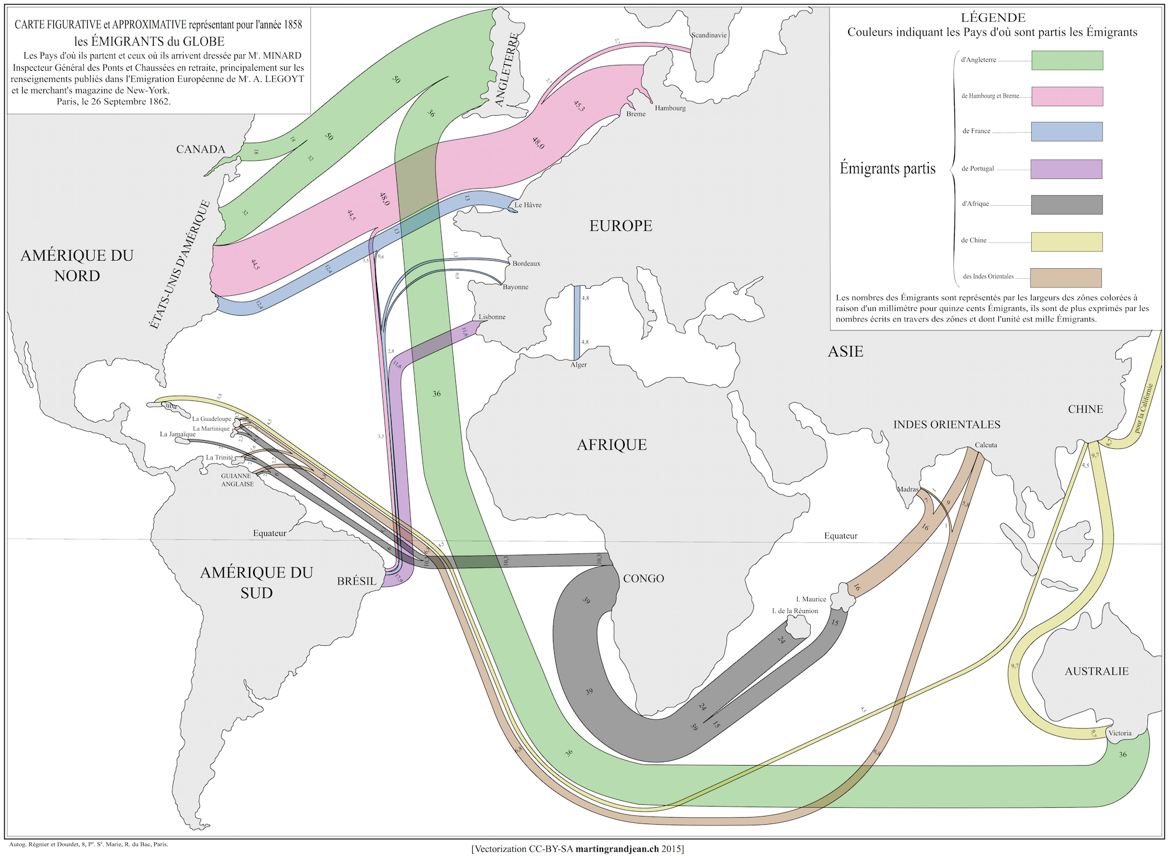
\includegraphics[width=1\linewidth]{img/minard}

\hypertarget{flowline-maps}{%
\subsection{Flowline Maps}\label{flowline-maps}}

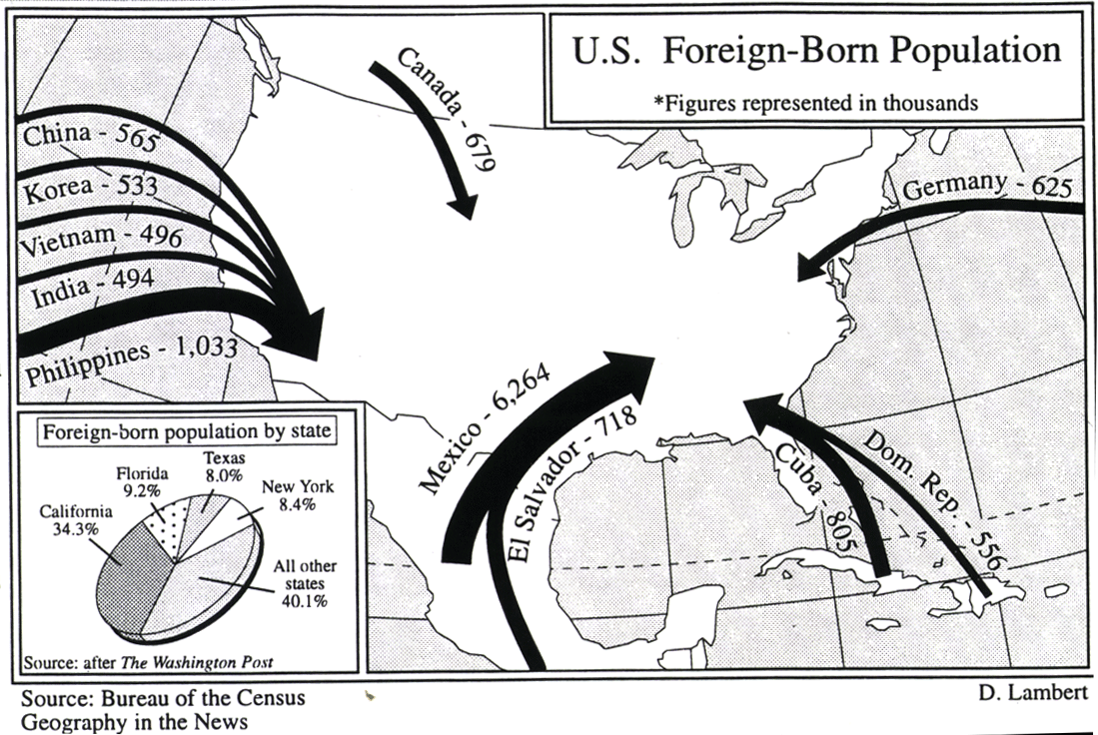
\includegraphics[width=1\linewidth]{img/lambert}

\hypertarget{criticised-new-york-times-refugee-flow-map}{%
\subsection{Criticised New York Times refugee flow map}\label{criticised-new-york-times-refugee-flow-map}}

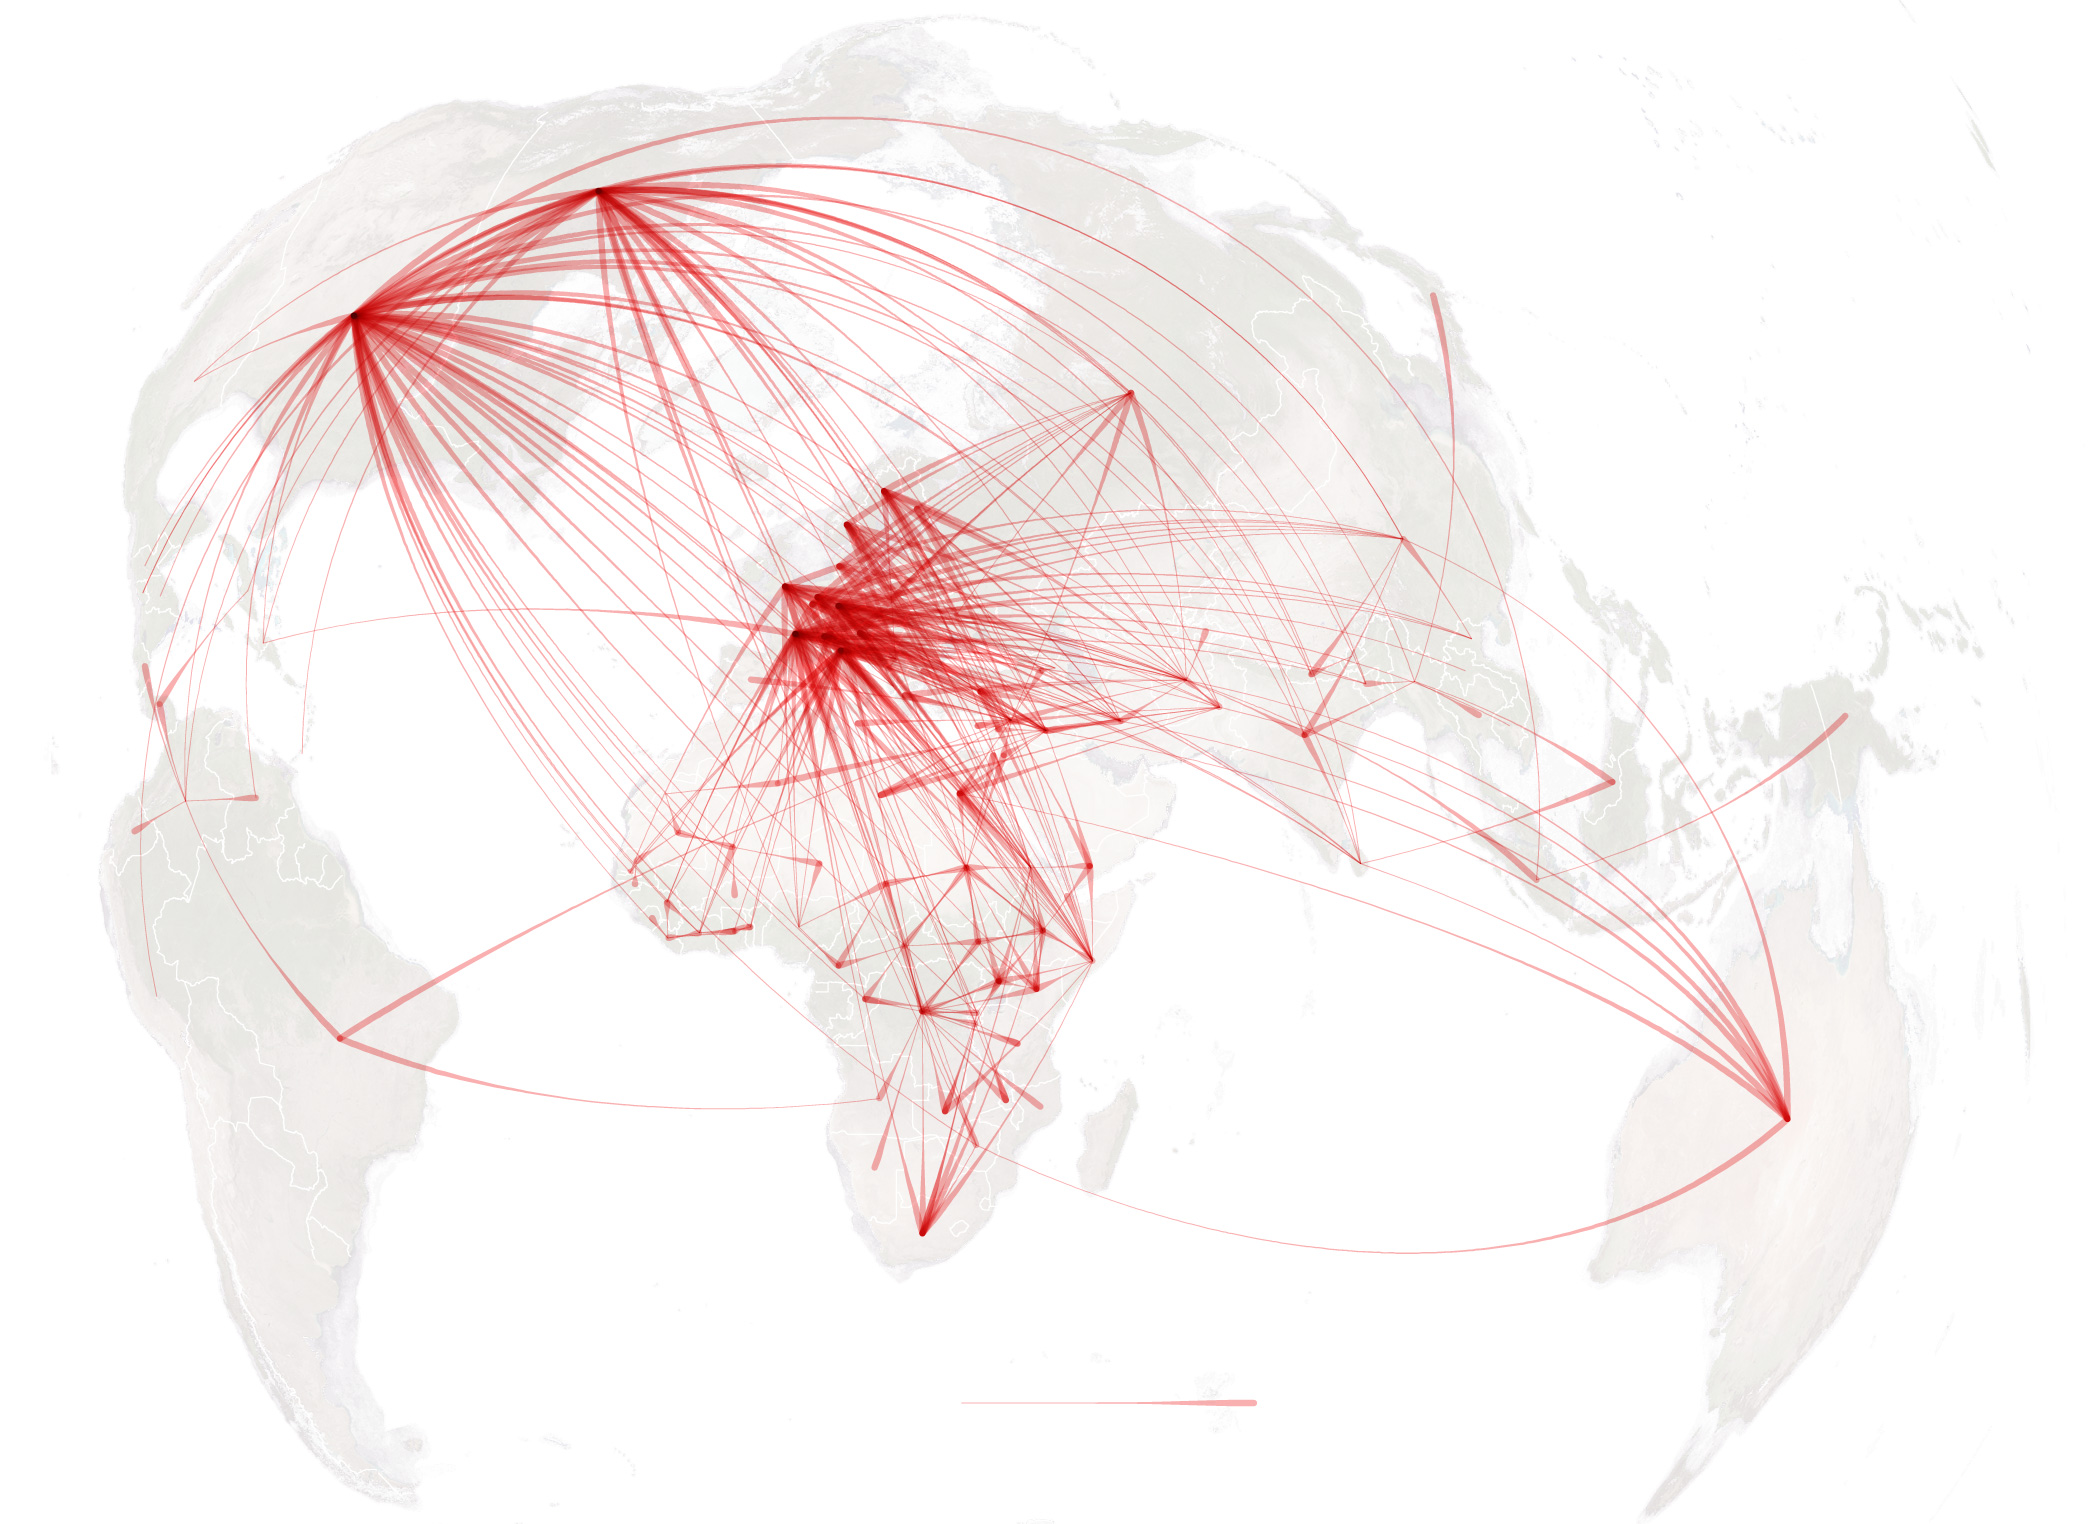
\includegraphics[width=1\linewidth]{img/refugee_flow_map-africa}

\hypertarget{martin-grandjeans-attempt-to-rectify}{%
\subsection{Martin Grandjean's attempt to rectify}\label{martin-grandjeans-attempt-to-rectify}}

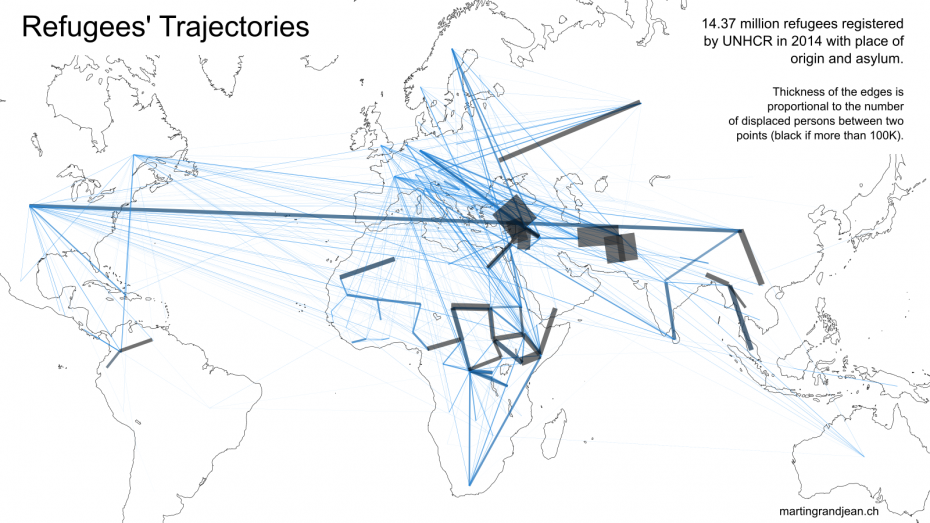
\includegraphics[width=1\linewidth]{img/Refugees-world-930x523}

\hypertarget{chord-diagram}{%
\section{Chord Diagram}\label{chord-diagram}}

\hypertarget{chord-diagrams}{%
\subsection{Chord Diagrams}\label{chord-diagrams}}

\begin{itemize}
\tightlist
\item
  First chord diagrams introduced by Martin Krzywinski in 2007.

  \begin{itemize}
  \tightlist
  \item
    \texttt{https://www.nytimes.com/imagepages/2007/01/22/science/20070123\_SCI\_ILLO.html}
  \end{itemize}
\item
  Used to facilitate the identification and analysis of similarities and differences arising from comparisons of genomes
\item
  Displays relationships between pairs of positions by the use of ribbons, which encode the position, size, and orientation of related genomic elements
\item
  Developed into Circos software in Perl by \citet{Krzywinski2009}

  \begin{itemize}
  \tightlist
  \item
    \texttt{http://circos.ca/}
  \end{itemize}
\end{itemize}

\hypertarget{new-york-times-2007}{%
\subsection{New York Times 2007}\label{new-york-times-2007}}

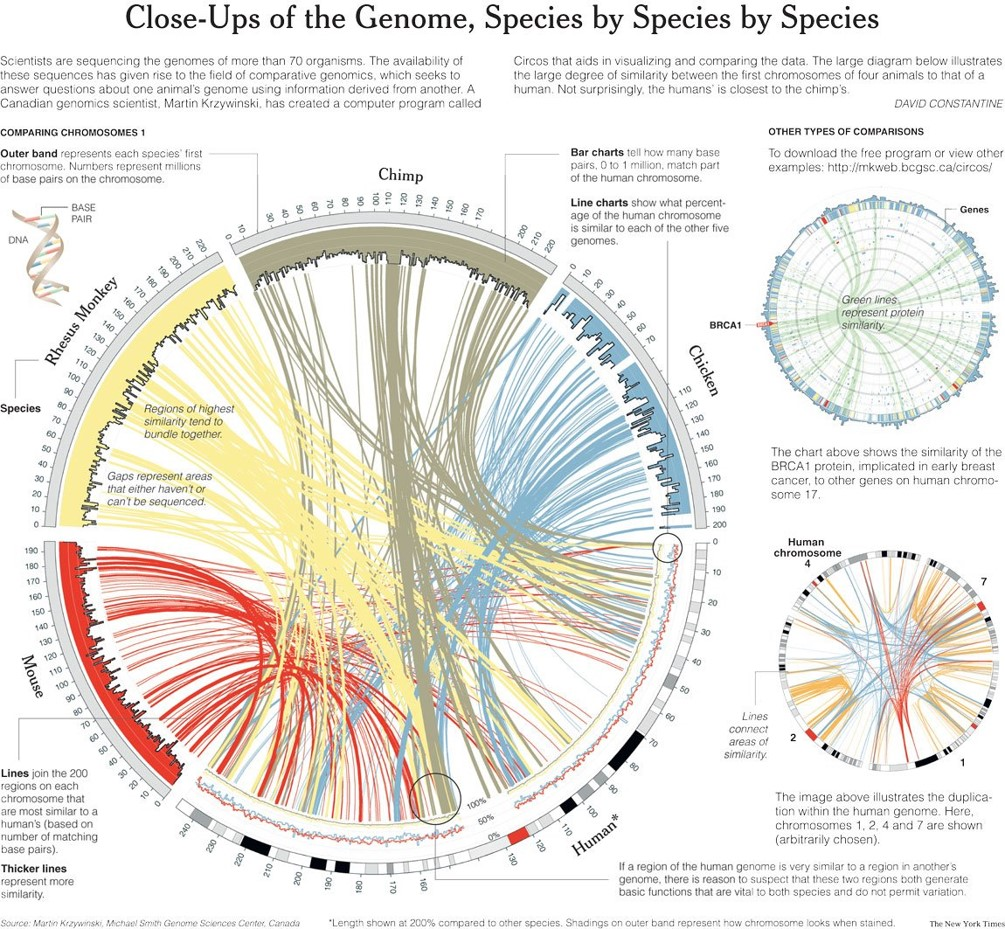
\includegraphics[width=1\linewidth]{img/nyt}

\hypertarget{chord-diagrams-with-migration-data}{%
\subsection{Chord Diagrams with Migration Data}\label{chord-diagrams-with-migration-data}}

\begin{itemize}
\tightlist
\item
  Interactive chord diagram plots introduced into rr.js library by Bostock
\item
  First used to illustrate migration patterns by data journalist Chris Walker in 2013

  \begin{itemize}
  \tightlist
  \item
    Mapping America's Restless Interstate Migration Without a Map \texttt{https://www.wired.com/2013/11/mapping-migration-without-a-map/}
  \end{itemize}
\item
  Does not show the direction of move until mouse-over.
\item
  Nikola Sander adapted Circos software to add directional indicators for flows

  \begin{itemize}
  \tightlist
  \item
    First used in \citet{Abel2014}. \emph{Quantifying Global International Migration Flows}. Science, 343 (6178).
  \item
    Interactive version at \texttt{http://download.gsb.bund.de/BIB/global\_flow/}
  \end{itemize}
\end{itemize}

\hypertarget{chord-diagrams-with-migration-data-1}{%
\subsection{Chord Diagrams with Migration Data}\label{chord-diagrams-with-migration-data-1}}

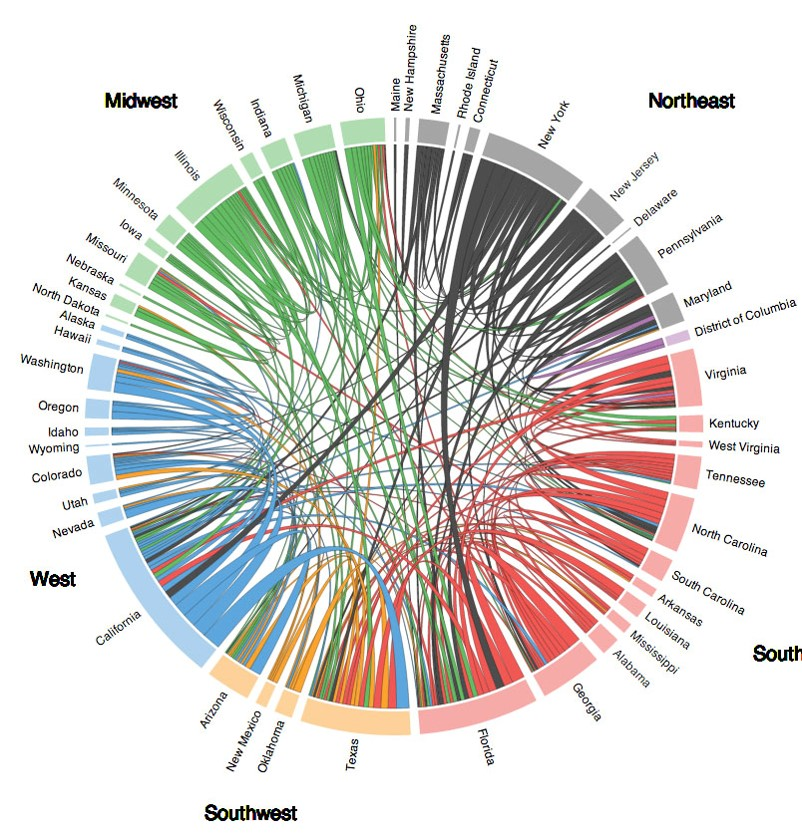
\includegraphics[width=1\linewidth]{img/walker}

\hypertarget{chord-diagrams-with-migration-data-2}{%
\subsection{Chord Diagrams with Migration Data}\label{chord-diagrams-with-migration-data-2}}

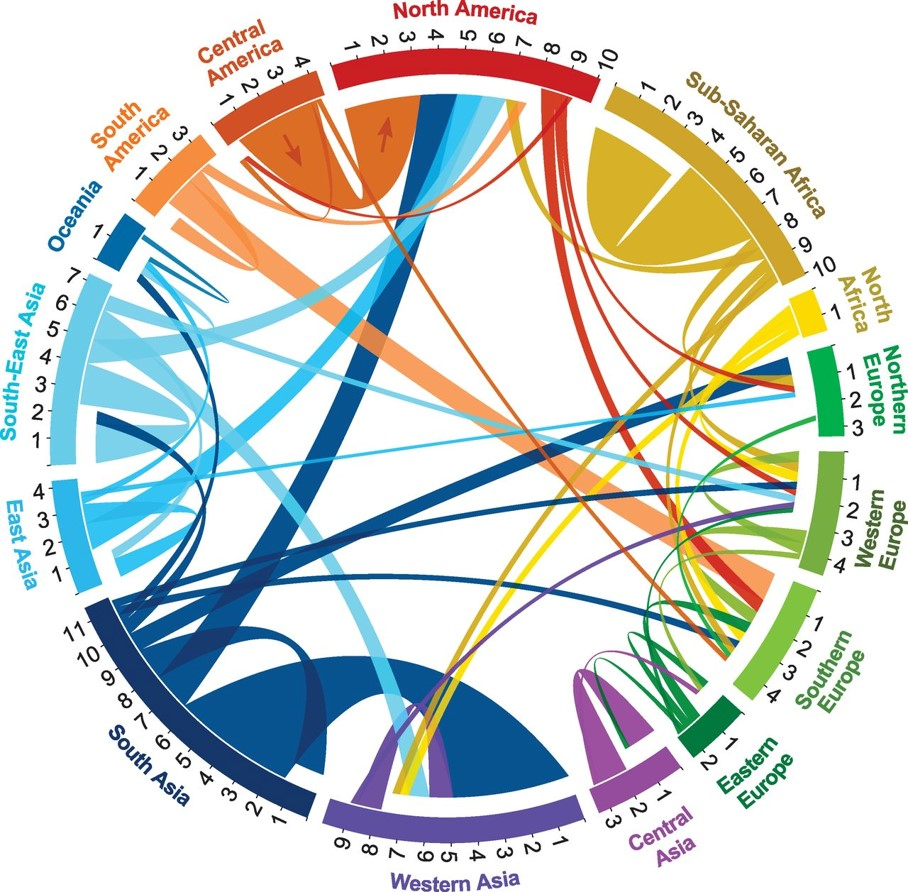
\includegraphics[width=1\linewidth]{img/sander}

\hypertarget{circlize}{%
\section{circlize}\label{circlize}}

\hypertarget{chord-diagrams-in-r}{%
\subsection{Chord Diagrams in R}\label{chord-diagrams-in-r}}

\begin{itemize}
\tightlist
\item
  Some drawbacks to the Circos based plots

  \begin{itemize}
  \tightlist
  \item
    Inflows plotted first on each sector
  \item
    Chords for smaller flows overlap larger flows
  \item
    Hides smallest flows
  \item
    Not easy to detect direction of flows
  \item
    Addition of direction arrows usually require some further touch using a second piece of software, e.g.~Photoshop or Illustrator

    \begin{itemize}
    \tightlist
    \item
      Problematic for replicability
    \end{itemize}
  \end{itemize}
\item
  In recent years a number of R packages that implement similar plots as the Circos software have appeared on CRAN
\item
  The \emph{circlize} R package by \citet{Gu2014} is perhaps the most complete and accessible for non-genomic data

  \begin{itemize}
  \tightlist
  \item
    Built on base R graphics package
  \end{itemize}
\item
  Includes a \texttt{chordDiagram()} function

  \begin{itemize}
  \tightlist
  \item
    Extensive documentation of the \texttt{chordDiagram()} function in \href{https://jokergoo.github.io/circlize_book/book/the-chorddiagram-function.html}{Chapters 13-15} of the circlize book.
  \end{itemize}
\end{itemize}

\hypertarget{un-international-migrant-stock-data-2020}{%
\subsection{UN international migrant stock data 2020}\label{un-international-migrant-stock-data-2020}}

\begin{Shaded}
\begin{Highlighting}[]
\FunctionTok{library}\NormalTok{(tidyverse)}
\NormalTok{un }\OtherTok{\textless{}{-}} \FunctionTok{read\_csv}\NormalTok{(}\AttributeTok{file =} \StringTok{"data/un\_desa\_ims\_tidy.csv"}\NormalTok{)}
\NormalTok{un}
\end{Highlighting}
\end{Shaded}

\begin{verbatim}
## # A tibble: 259,357 x 6
##     year     stock por_name por_code pob_name           pob_code
##    <dbl>     <dbl> <chr>       <dbl> <chr>                 <dbl>
##  1  1990 152986157 WORLD         900 WORLD                   900
##  2  1995 161289976 WORLD         900 WORLD                   900
##  3  2000 173230585 WORLD         900 WORLD                   900
##  4  2005 191446828 WORLD         900 WORLD                   900
##  5  2010 220983187 WORLD         900 WORLD                   900
##  6  2015 247958644 WORLD         900 WORLD                   900
##  7  2020 280598105 WORLD         900 WORLD                   900
##  8  1990  15334807 WORLD         900 Sub-Saharan Africa      947
##  9  1995  16488973 WORLD         900 Sub-Saharan Africa      947
## 10  2000  15638014 WORLD         900 Sub-Saharan Africa      947
## # ... with 259,347 more rows
\end{verbatim}

\hypertarget{un-international-migrant-stock-data-2020-1}{%
\subsection{UN international migrant stock data 2020}\label{un-international-migrant-stock-data-2020-1}}

\begin{itemize}
\tightlist
\item
  Use continent to continent flows in 2020
\end{itemize}

\begin{Shaded}
\begin{Highlighting}[]
\CommentTok{\# codes for contents}
\NormalTok{cc }\OtherTok{\textless{}{-}} \FunctionTok{c}\NormalTok{(}\DecValTok{903}\NormalTok{, }\DecValTok{935}\NormalTok{, }\DecValTok{908}\NormalTok{, }\DecValTok{904}\NormalTok{, }\DecValTok{905}\NormalTok{, }\DecValTok{909}\NormalTok{)}
\NormalTok{d }\OtherTok{\textless{}{-}}\NormalTok{ un }\SpecialCharTok{\%\textgreater{}\%}
  \FunctionTok{filter}\NormalTok{(por\_code }\SpecialCharTok{\%in\%}\NormalTok{ cc, }
\NormalTok{         pob\_code }\SpecialCharTok{\%in\%}\NormalTok{ cc,}
\NormalTok{         year }\SpecialCharTok{==} \DecValTok{2020}\NormalTok{)}
\NormalTok{d}
\end{Highlighting}
\end{Shaded}

\begin{verbatim}
## # A tibble: 36 x 6
##     year    stock por_name por_code pob_name                        pob_code
##    <dbl>    <dbl> <chr>       <dbl> <chr>                              <dbl>
##  1  2020 20917565 AFRICA        903 AFRICA                               903
##  2  2020  1207631 AFRICA        903 ASIA                                 935
##  3  2020   648455 AFRICA        903 EUROPE                               908
##  4  2020    32524 AFRICA        903 LATIN AMERICA AND THE CARIBBEAN      904
##  5  2020    53563 AFRICA        903 NORTHERN AMERICA                     905
##  6  2020    14483 AFRICA        903 OCEANIA                              909
##  7  2020  4720103 ASIA          935 AFRICA                               903
##  8  2020 68497762 ASIA          935 ASIA                                 935
##  9  2020  7169630 ASIA          935 EUROPE                               908
## 10  2020   414658 ASIA          935 LATIN AMERICA AND THE CARIBBEAN      904
## # ... with 26 more rows
\end{verbatim}

\hypertarget{un-international-migrant-stock-data-2020-2}{%
\subsection{UN international migrant stock data 2020}\label{un-international-migrant-stock-data-2020-2}}

\begin{itemize}
\tightlist
\item
  Remove within continent stocks (will dominate the plot) and focus on inter-continent migrants
\end{itemize}

\begin{Shaded}
\begin{Highlighting}[]
\NormalTok{d }\OtherTok{\textless{}{-}}\NormalTok{ d }\SpecialCharTok{\%\textgreater{}\%}
  \FunctionTok{rename}\NormalTok{(}\AttributeTok{orig =}\NormalTok{ pob\_name,}
         \AttributeTok{dest =}\NormalTok{ por\_name) }\SpecialCharTok{\%\textgreater{}\%}
  \FunctionTok{filter}\NormalTok{(orig }\SpecialCharTok{!=}\NormalTok{ dest) }\SpecialCharTok{\%\textgreater{}\%}
  \FunctionTok{select}\NormalTok{(}\SpecialCharTok{{-}}\FunctionTok{contains}\NormalTok{(}\StringTok{"code"}\NormalTok{))}
\NormalTok{d}
\end{Highlighting}
\end{Shaded}

\begin{verbatim}
## # A tibble: 30 x 4
##     year   stock dest   orig                           
##    <dbl>   <dbl> <chr>  <chr>                          
##  1  2020 1207631 AFRICA ASIA                           
##  2  2020  648455 AFRICA EUROPE                         
##  3  2020   32524 AFRICA LATIN AMERICA AND THE CARIBBEAN
##  4  2020   53563 AFRICA NORTHERN AMERICA               
##  5  2020   14483 AFRICA OCEANIA                        
##  6  2020 4720103 ASIA   AFRICA                         
##  7  2020 7169630 ASIA   EUROPE                         
##  8  2020  414658 ASIA   LATIN AMERICA AND THE CARIBBEAN
##  9  2020  538199 ASIA   NORTHERN AMERICA               
## 10  2020  101725 ASIA   OCEANIA                        
## # ... with 20 more rows
\end{verbatim}

\hypertarget{default-chorddiagram}{%
\subsection{\texorpdfstring{Default \texttt{chordDiagram()}}{Default chordDiagram()}}\label{default-chorddiagram}}

\begin{itemize}
\tightlist
\item
  The \texttt{chordDiagram()} function can take either a \texttt{matrix} or \texttt{data.frame} object as first argument \texttt{x} for the data.
\item
  I prefer the latter as they are much easier to create and manipulate (using \emph{dplyr} and other \emph{tidyverse} packages).

  \begin{itemize}
  \tightlist
  \item
    When using a \texttt{data.frame}, the first three columns should correspond to the origin, destination and size of connection.
  \item
    Columns can take any name, but must be in that order.
  \item
    Will also work with \texttt{tbl\_df} (tibble)
  \end{itemize}
\item
  Many options in \texttt{chordDiagram()}, that by default are not ideal for displaying migration data
\end{itemize}

\begin{Shaded}
\begin{Highlighting}[]
\FunctionTok{library}\NormalTok{(circlize)}
\CommentTok{\# first three columns not origin, destination, connection (in that order)}
\FunctionTok{chordDiagram}\NormalTok{(}\AttributeTok{x =}\NormalTok{ d)}
\end{Highlighting}
\end{Shaded}

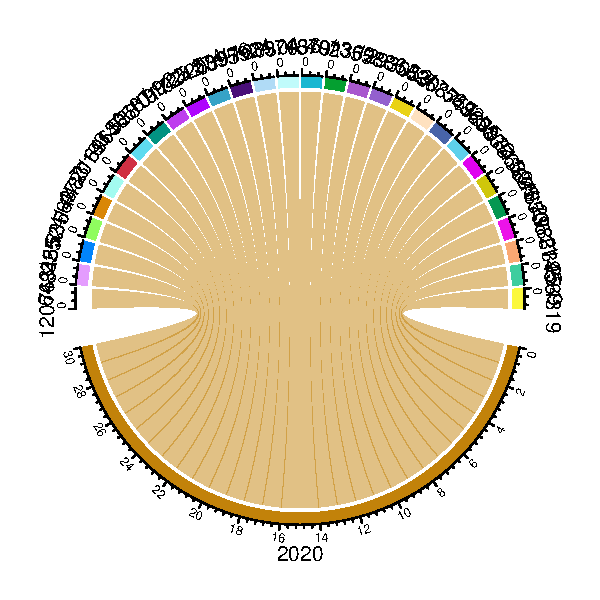
\includegraphics{_main_files/figure-latex/cd-default-1.pdf}

\hypertarget{default-chorddiagram-1}{%
\subsection{\texorpdfstring{Default \texttt{chordDiagram()}}{Default chordDiagram()}}\label{default-chorddiagram-1}}

\begin{itemize}
\tightlist
\item
  Move the \texttt{orig}, \texttt{dest} and \texttt{stock} columns to the left of the data frame using the \texttt{relocate()} function in the \emph{dplyr} package
\end{itemize}

\begin{Shaded}
\begin{Highlighting}[]
\NormalTok{d }\OtherTok{\textless{}{-}} \FunctionTok{relocate}\NormalTok{(d, orig, dest, stock)}
\NormalTok{d}
\end{Highlighting}
\end{Shaded}

\begin{verbatim}
## # A tibble: 30 x 4
##    orig                            dest     stock  year
##    <chr>                           <chr>    <dbl> <dbl>
##  1 ASIA                            AFRICA 1207631  2020
##  2 EUROPE                          AFRICA  648455  2020
##  3 LATIN AMERICA AND THE CARIBBEAN AFRICA   32524  2020
##  4 NORTHERN AMERICA                AFRICA   53563  2020
##  5 OCEANIA                         AFRICA   14483  2020
##  6 AFRICA                          ASIA   4720103  2020
##  7 EUROPE                          ASIA   7169630  2020
##  8 LATIN AMERICA AND THE CARIBBEAN ASIA    414658  2020
##  9 NORTHERN AMERICA                ASIA    538199  2020
## 10 OCEANIA                         ASIA    101725  2020
## # ... with 20 more rows
\end{verbatim}

\begin{Shaded}
\begin{Highlighting}[]
\FunctionTok{chordDiagram}\NormalTok{(}\AttributeTok{x =}\NormalTok{ d)}
\end{Highlighting}
\end{Shaded}

\begin{verbatim}
## There are more than one numeric columns in the data frame. Take the
## first two numeric columns and draw the link ends with unequal width.
## 
## Type `circos.par$message = FALSE` to suppress the message.
\end{verbatim}

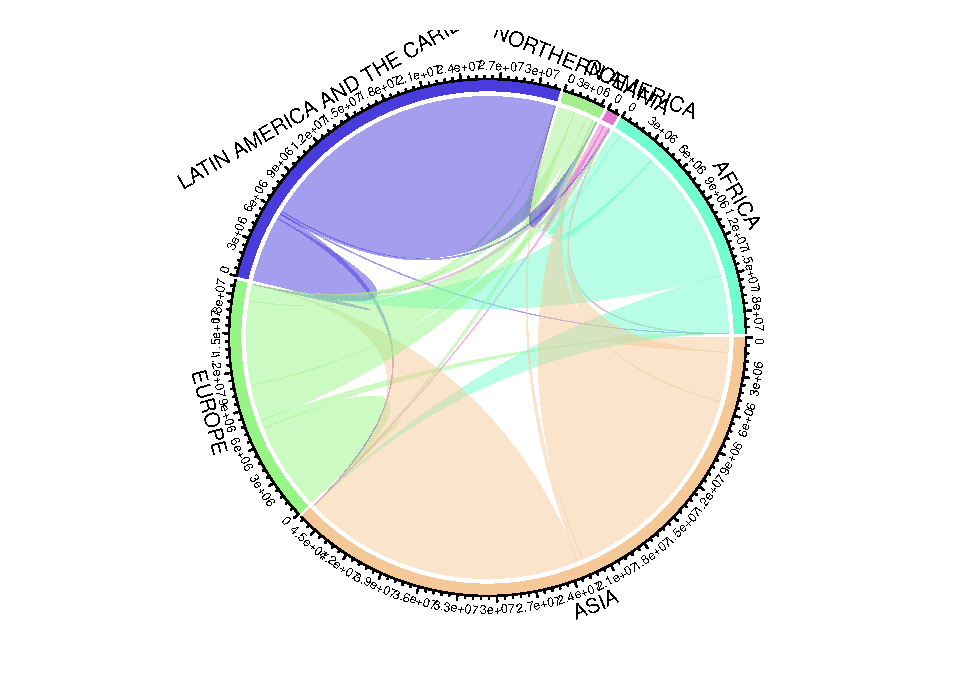
\includegraphics{_main_files/figure-latex/cd-col-order-1.pdf}

\hypertarget{default-chorddiagram-2}{%
\subsection{\texorpdfstring{Default \texttt{chordDiagram()}}{Default chordDiagram()}}\label{default-chorddiagram-2}}

\begin{itemize}
\tightlist
\item
  Avoid chord link ends with unequal widths at each base by using only one numeric column in \texttt{d}
\end{itemize}

\begin{Shaded}
\begin{Highlighting}[]
\NormalTok{d }\OtherTok{\textless{}{-}} \FunctionTok{select}\NormalTok{(d, orig, dest, stock)}
\NormalTok{d}
\end{Highlighting}
\end{Shaded}

\begin{verbatim}
## # A tibble: 30 x 3
##    orig                            dest     stock
##    <chr>                           <chr>    <dbl>
##  1 ASIA                            AFRICA 1207631
##  2 EUROPE                          AFRICA  648455
##  3 LATIN AMERICA AND THE CARIBBEAN AFRICA   32524
##  4 NORTHERN AMERICA                AFRICA   53563
##  5 OCEANIA                         AFRICA   14483
##  6 AFRICA                          ASIA   4720103
##  7 EUROPE                          ASIA   7169630
##  8 LATIN AMERICA AND THE CARIBBEAN ASIA    414658
##  9 NORTHERN AMERICA                ASIA    538199
## 10 OCEANIA                         ASIA    101725
## # ... with 20 more rows
\end{verbatim}

\begin{Shaded}
\begin{Highlighting}[]
\FunctionTok{chordDiagram}\NormalTok{(}\AttributeTok{x =}\NormalTok{ d)}
\end{Highlighting}
\end{Shaded}

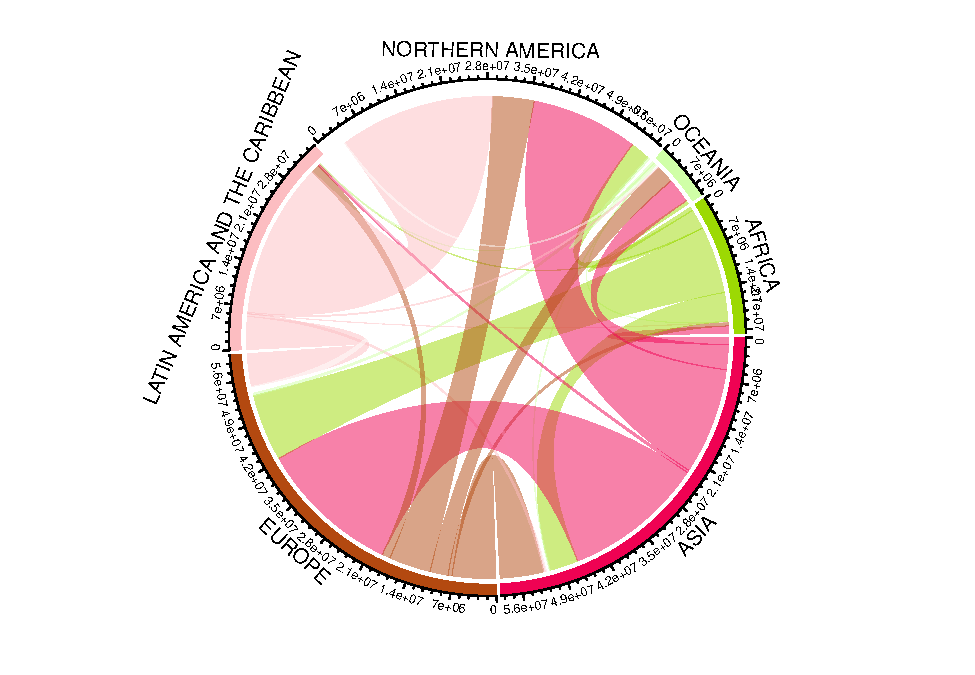
\includegraphics{_main_files/figure-latex/cd-column3-1.pdf}

\hypertarget{sectors}{%
\section{Sectors}\label{sectors}}

\hypertarget{sector-axis}{%
\subsection{Sector Axis}\label{sector-axis}}

\begin{itemize}
\tightlist
\item
  Edit the bilateral counts to a sensible scale to ensure the axis labels are legible.
\end{itemize}

\begin{Shaded}
\begin{Highlighting}[]
\NormalTok{d }\OtherTok{\textless{}{-}} \FunctionTok{mutate}\NormalTok{(d, }\AttributeTok{stock =}\NormalTok{ stock}\SpecialCharTok{/}\FloatTok{1e6}\NormalTok{)}
\NormalTok{d}
\end{Highlighting}
\end{Shaded}

\begin{verbatim}
## # A tibble: 30 x 3
##    orig                            dest    stock
##    <chr>                           <chr>   <dbl>
##  1 ASIA                            AFRICA 1.21  
##  2 EUROPE                          AFRICA 0.648 
##  3 LATIN AMERICA AND THE CARIBBEAN AFRICA 0.0325
##  4 NORTHERN AMERICA                AFRICA 0.0536
##  5 OCEANIA                         AFRICA 0.0145
##  6 AFRICA                          ASIA   4.72  
##  7 EUROPE                          ASIA   7.17  
##  8 LATIN AMERICA AND THE CARIBBEAN ASIA   0.415 
##  9 NORTHERN AMERICA                ASIA   0.538 
## 10 OCEANIA                         ASIA   0.102 
## # ... with 20 more rows
\end{verbatim}

\begin{Shaded}
\begin{Highlighting}[]
\FunctionTok{chordDiagram}\NormalTok{(}\AttributeTok{x =}\NormalTok{ d)}
\end{Highlighting}
\end{Shaded}

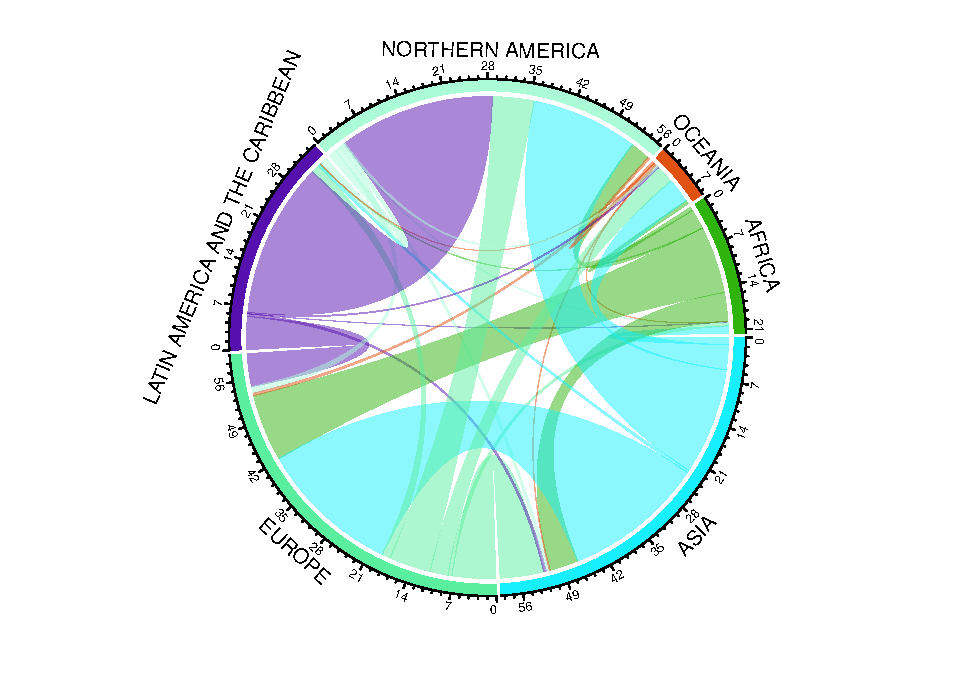
\includegraphics{_main_files/figure-latex/cd-axis-1.pdf}

\hypertarget{sector-ordering}{%
\subsection{Sector ordering}\label{sector-ordering}}

\begin{itemize}
\tightlist
\item
  Sector ordering is alphabetical by default
\item
  Can specify order using \texttt{order} argument and pass a vector
\item
  Try to order so that neighboring regions are next each other
\end{itemize}

\begin{Shaded}
\begin{Highlighting}[]
\NormalTok{r }\OtherTok{\textless{}{-}} \FunctionTok{tibble}\NormalTok{(}\AttributeTok{reg =} \FunctionTok{union}\NormalTok{(d}\SpecialCharTok{$}\NormalTok{orig, d}\SpecialCharTok{$}\NormalTok{dest))}
\NormalTok{r}
\end{Highlighting}
\end{Shaded}

\begin{verbatim}
## # A tibble: 6 x 1
##   reg                            
##   <chr>                          
## 1 ASIA                           
## 2 EUROPE                         
## 3 LATIN AMERICA AND THE CARIBBEAN
## 4 NORTHERN AMERICA               
## 5 OCEANIA                        
## 6 AFRICA
\end{verbatim}

\hypertarget{sector-ordering-1}{%
\subsection{Sector ordering}\label{sector-ordering-1}}

\begin{Shaded}
\begin{Highlighting}[]
\NormalTok{r }\OtherTok{\textless{}{-}}\NormalTok{ r }\SpecialCharTok{\%\textgreater{}\%}
  \FunctionTok{mutate}\NormalTok{(}\AttributeTok{reg\_order =} \FunctionTok{c}\NormalTok{(}\DecValTok{4}\NormalTok{, }\DecValTok{3}\NormalTok{, }\DecValTok{6}\NormalTok{, }\DecValTok{1}\NormalTok{, }\DecValTok{5}\NormalTok{, }\DecValTok{2}\NormalTok{)) }\SpecialCharTok{\%\textgreater{}\%}
  \FunctionTok{arrange}\NormalTok{(reg\_order)}
\NormalTok{r}
\end{Highlighting}
\end{Shaded}

\begin{verbatim}
## # A tibble: 6 x 2
##   reg                             reg_order
##   <chr>                               <dbl>
## 1 NORTHERN AMERICA                        1
## 2 AFRICA                                  2
## 3 EUROPE                                  3
## 4 ASIA                                    4
## 5 OCEANIA                                 5
## 6 LATIN AMERICA AND THE CARIBBEAN         6
\end{verbatim}

\begin{Shaded}
\begin{Highlighting}[]
\CommentTok{\# order sectors}
\FunctionTok{chordDiagram}\NormalTok{(}\AttributeTok{x =}\NormalTok{ d, }\AttributeTok{order =}\NormalTok{ r}\SpecialCharTok{$}\NormalTok{reg)}
\end{Highlighting}
\end{Shaded}

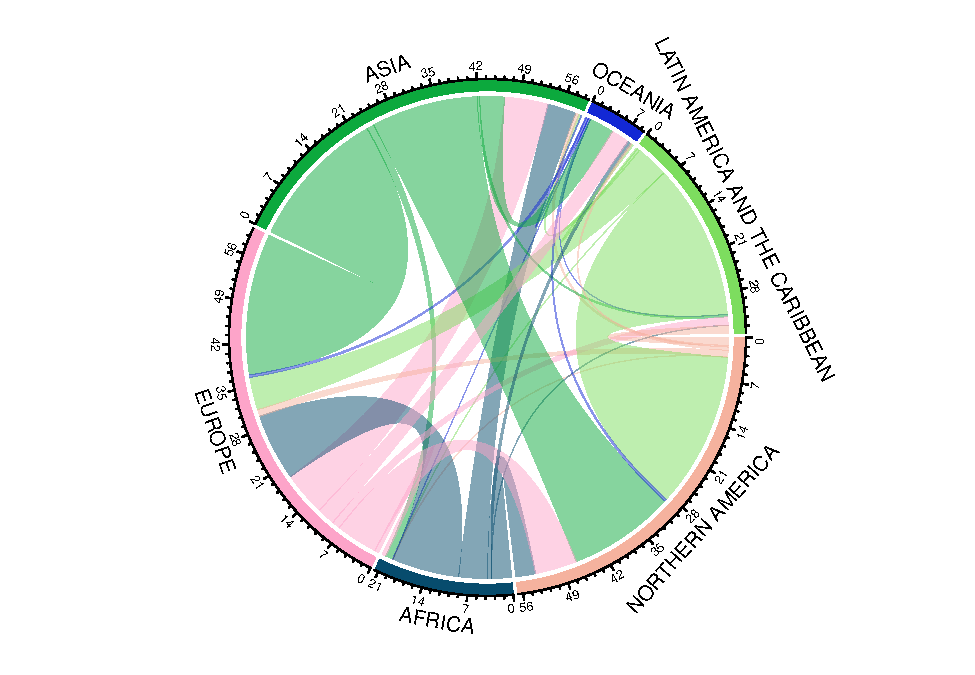
\includegraphics{_main_files/figure-latex/cd-sector-1.pdf}

\hypertarget{orientation-and-gaps}{%
\subsection{Orientation and gaps}\label{orientation-and-gaps}}

\begin{itemize}
\tightlist
\item
  The \texttt{circos.par()} function controls the overall layout parameters of the graphic display
\item
  Use \texttt{circos.par()} to set

  \begin{itemize}
  \tightlist
  \item
    \texttt{gap.degree} the degree of gaps between sectors are set - default \texttt{gap.degree\ =\ 1}
  \item
    \texttt{start.degree} the degree from three o'clock where the first sector appears - default \texttt{start.degree\ =\ 0}
  \end{itemize}
\item
  Anything set via \texttt{circos.par()} will be fixed for all remaining pots
\item
  Reset to default graphic parameters using \texttt{circos.clear()} or overwrite with new \texttt{circos.par()}
\end{itemize}

\begin{Shaded}
\begin{Highlighting}[]
\CommentTok{\# increase gaps}
\FunctionTok{circos.par}\NormalTok{(}\AttributeTok{gap.degree =} \DecValTok{5}\NormalTok{)}
\FunctionTok{chordDiagram}\NormalTok{(}\AttributeTok{x =}\NormalTok{ d, }\AttributeTok{order =}\NormalTok{ r}\SpecialCharTok{$}\NormalTok{reg)}
\end{Highlighting}
\end{Shaded}

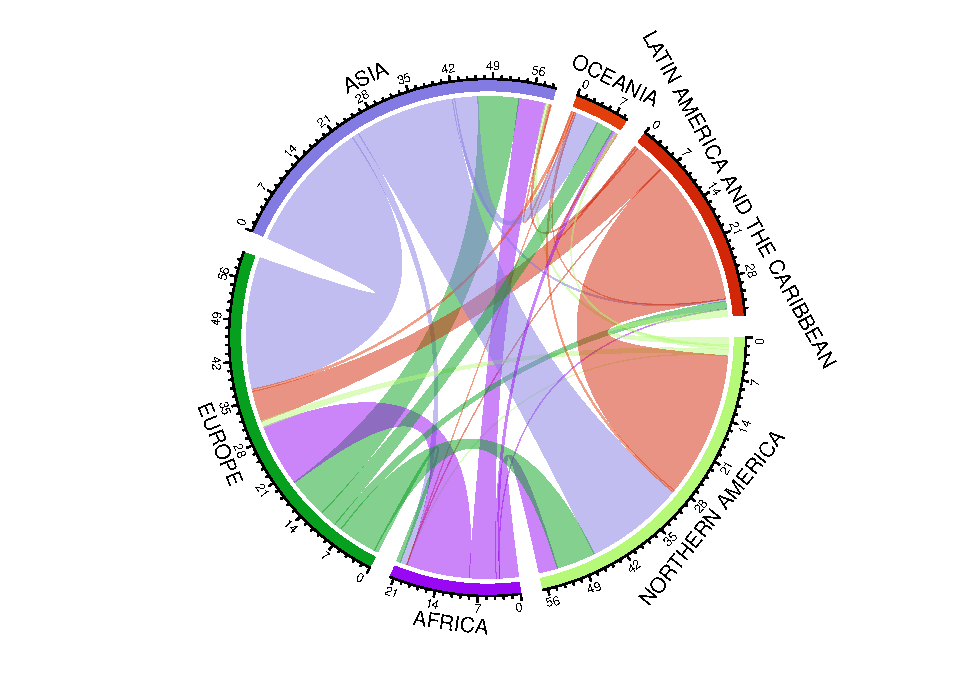
\includegraphics{_main_files/figure-latex/cd-gap-1.pdf}

\begin{Shaded}
\begin{Highlighting}[]
\CommentTok{\# rotate}
\FunctionTok{circos.par}\NormalTok{(}\AttributeTok{start.degree =} \DecValTok{90}\NormalTok{)}
\FunctionTok{chordDiagram}\NormalTok{(}\AttributeTok{x =}\NormalTok{ d, }\AttributeTok{order =}\NormalTok{ r}\SpecialCharTok{$}\NormalTok{reg)}
\end{Highlighting}
\end{Shaded}

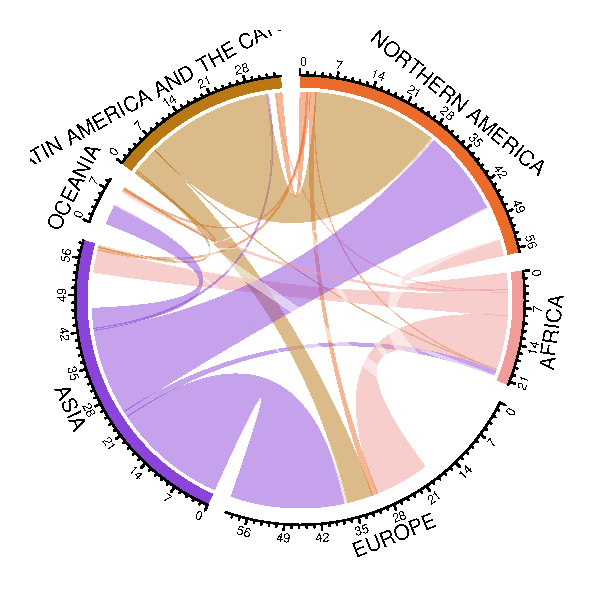
\includegraphics{_main_files/figure-latex/cd-gap-2.pdf}

\hypertarget{colour}{%
\section{Colour}\label{colour}}

\hypertarget{sector-colours}{%
\subsection{Sector colours}\label{sector-colours}}

\begin{itemize}
\tightlist
\item
  Colours are randomly generated (will change every time you plot)
\item
  Can set to a choice using either:

  \begin{itemize}
  \tightlist
  \item
    \texttt{grid.col} corresponding to sectors (regions/countries/areas)
  \item
    \texttt{transparency} set by default to 0.5
  \end{itemize}
\end{itemize}

\begin{Shaded}
\begin{Highlighting}[]
\NormalTok{r }\OtherTok{\textless{}{-}}\NormalTok{ r }\SpecialCharTok{\%\textgreater{}\%}
  \FunctionTok{mutate}\NormalTok{(}\AttributeTok{col1 =} \FunctionTok{c}\NormalTok{(}\StringTok{"black"}\NormalTok{, }\StringTok{"gold"}\NormalTok{, }\StringTok{"orange"}\NormalTok{, }\StringTok{"blue"}\NormalTok{, }\StringTok{"purple"}\NormalTok{, }\StringTok{"red"}\NormalTok{))}
\NormalTok{r}
\end{Highlighting}
\end{Shaded}

\begin{verbatim}
## # A tibble: 6 x 3
##   reg                             reg_order col1  
##   <chr>                               <dbl> <chr> 
## 1 NORTHERN AMERICA                        1 black 
## 2 AFRICA                                  2 gold  
## 3 EUROPE                                  3 orange
## 4 ASIA                                    4 blue  
## 5 OCEANIA                                 5 purple
## 6 LATIN AMERICA AND THE CARIBBEAN         6 red
\end{verbatim}

\begin{Shaded}
\begin{Highlighting}[]
\FunctionTok{chordDiagram}\NormalTok{(}\AttributeTok{x =}\NormalTok{ d, }\AttributeTok{order =}\NormalTok{ r}\SpecialCharTok{$}\NormalTok{reg, }\AttributeTok{grid.col =}\NormalTok{ r}\SpecialCharTok{$}\NormalTok{col1)}
\end{Highlighting}
\end{Shaded}

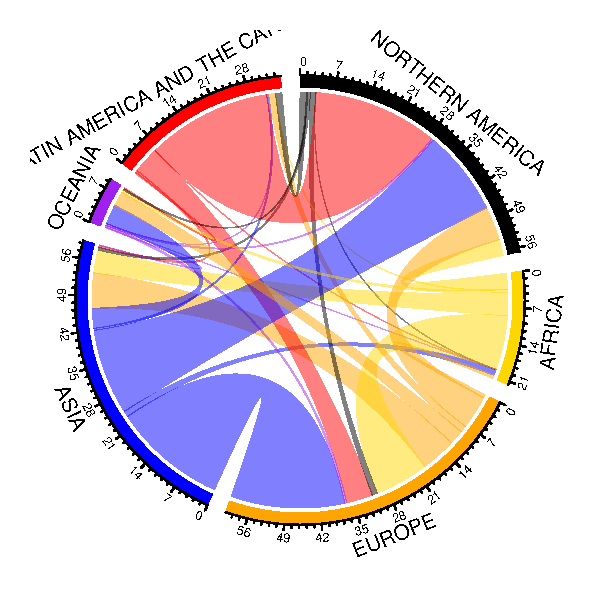
\includegraphics{_main_files/figure-latex/cd-col1-1.pdf}

\hypertarget{sector-colour}{%
\subsection{Sector colour}\label{sector-colour}}

\begin{itemize}
\tightlist
\item
  Can use the \emph{RColourBrewer} package to generate palettes (maximum of 9 colours)

  \begin{itemize}
  \tightlist
  \item
    Based on \texttt{https://colorbrewer2.org/}
  \end{itemize}
\end{itemize}

\begin{Shaded}
\begin{Highlighting}[]
\FunctionTok{library}\NormalTok{(RColorBrewer)}
\NormalTok{r }\OtherTok{\textless{}{-}}\NormalTok{ r }\SpecialCharTok{\%\textgreater{}\%}
  \FunctionTok{mutate}\NormalTok{(}\AttributeTok{col2 =} \FunctionTok{brewer.pal}\NormalTok{(}\AttributeTok{n =} \DecValTok{6}\NormalTok{, }\AttributeTok{name =} \StringTok{"Set1"}\NormalTok{),}
         \AttributeTok{col3 =} \FunctionTok{c}\NormalTok{(}\StringTok{"Red"}\NormalTok{, }\FunctionTok{rep}\NormalTok{(}\StringTok{"Grey"}\NormalTok{, }\AttributeTok{times =} \DecValTok{5}\NormalTok{)))}
\NormalTok{r}
\end{Highlighting}
\end{Shaded}

\begin{verbatim}
## # A tibble: 6 x 5
##   reg                             reg_order col1   col2    col3 
##   <chr>                               <dbl> <chr>  <chr>   <chr>
## 1 NORTHERN AMERICA                        1 black  #E41A1C Red  
## 2 AFRICA                                  2 gold   #377EB8 Grey 
## 3 EUROPE                                  3 orange #4DAF4A Grey 
## 4 ASIA                                    4 blue   #984EA3 Grey 
## 5 OCEANIA                                 5 purple #FF7F00 Grey 
## 6 LATIN AMERICA AND THE CARIBBEAN         6 red    #FFFF33 Grey
\end{verbatim}

\begin{Shaded}
\begin{Highlighting}[]
\FunctionTok{chordDiagram}\NormalTok{(}\AttributeTok{x =}\NormalTok{ d, }\AttributeTok{order =}\NormalTok{ r}\SpecialCharTok{$}\NormalTok{reg, }\AttributeTok{grid.col =}\NormalTok{ r}\SpecialCharTok{$}\NormalTok{col2)}
\end{Highlighting}
\end{Shaded}

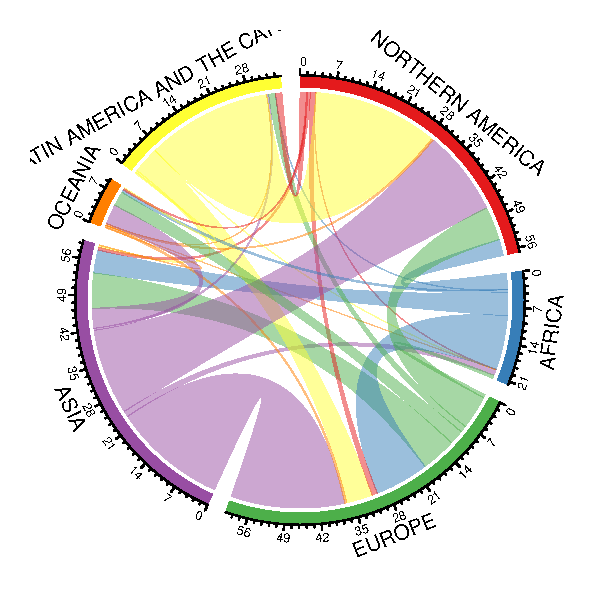
\includegraphics{_main_files/figure-latex/cd-col2-1.pdf}

\begin{Shaded}
\begin{Highlighting}[]
\FunctionTok{chordDiagram}\NormalTok{(}\AttributeTok{x =}\NormalTok{ d, }\AttributeTok{order =}\NormalTok{ r}\SpecialCharTok{$}\NormalTok{reg, }\AttributeTok{grid.col =}\NormalTok{ r}\SpecialCharTok{$}\NormalTok{col2, }\AttributeTok{transparency =} \FloatTok{0.25}\NormalTok{)}
\end{Highlighting}
\end{Shaded}

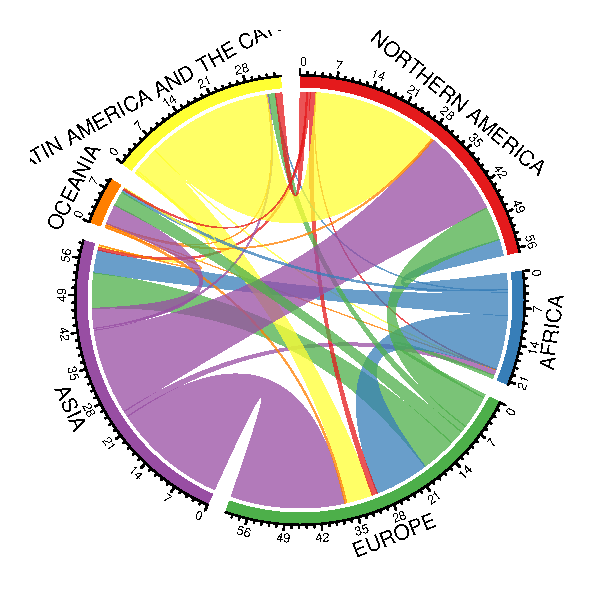
\includegraphics{_main_files/figure-latex/cd-col2-2.pdf}

\begin{Shaded}
\begin{Highlighting}[]
\FunctionTok{chordDiagram}\NormalTok{(}\AttributeTok{x =}\NormalTok{ d, }\AttributeTok{order =}\NormalTok{ r}\SpecialCharTok{$}\NormalTok{reg, }\AttributeTok{grid.col =}\NormalTok{ r}\SpecialCharTok{$}\NormalTok{col3)}
\end{Highlighting}
\end{Shaded}

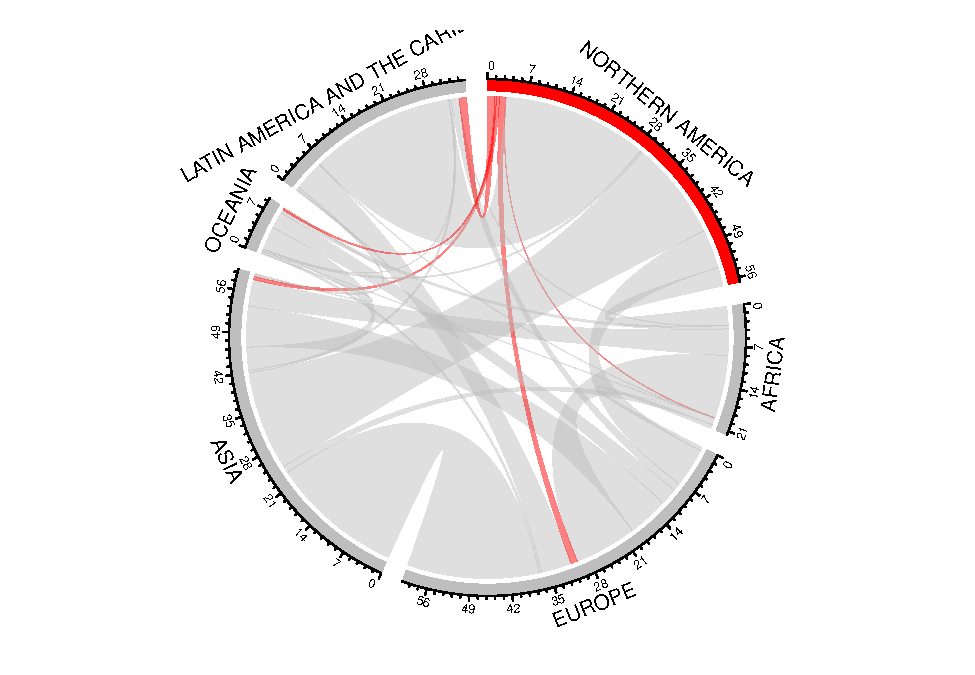
\includegraphics{_main_files/figure-latex/cd-col2-3.pdf}

\hypertarget{chord-colours}{%
\subsection{Chord colours}\label{chord-colours}}

\begin{itemize}
\tightlist
\item
  Chord colours follow the origin sector. We can specify different colours using

  \begin{itemize}
  \tightlist
  \item
    \texttt{col} corresponding to links (bilateral migration data)
  \item
    \texttt{link.visible} will hide particular chords
  \end{itemize}
\end{itemize}

\begin{Shaded}
\begin{Highlighting}[]
\NormalTok{d }\OtherTok{\textless{}{-}}\NormalTok{ d }\SpecialCharTok{\%\textgreater{}\%}
  \CommentTok{\# highlight Asia to Europe flows}
  \FunctionTok{mutate}\NormalTok{(}\AttributeTok{link\_col1 =} \FunctionTok{ifelse}\NormalTok{(}\AttributeTok{test =}\NormalTok{ orig }\SpecialCharTok{==} \StringTok{"ASIA"} \SpecialCharTok{\&}\NormalTok{ dest }\SpecialCharTok{==} \StringTok{"EUROPE"}\NormalTok{,}
                            \AttributeTok{yes =} \StringTok{"black"}\NormalTok{, }\AttributeTok{no =} \StringTok{"grey"}\NormalTok{),}
         \CommentTok{\# show only flows out or into Asia}
         \AttributeTok{show\_link =}\NormalTok{ orig }\SpecialCharTok{==} \StringTok{"ASIA"} \SpecialCharTok{|}\NormalTok{ dest }\SpecialCharTok{==} \StringTok{"ASIA"}\NormalTok{)}
\NormalTok{d}
\end{Highlighting}
\end{Shaded}

\begin{verbatim}
## # A tibble: 30 x 5
##    orig                            dest    stock link_col1 show_link
##    <chr>                           <chr>   <dbl> <chr>     <lgl>    
##  1 ASIA                            AFRICA 1.21   grey      TRUE     
##  2 EUROPE                          AFRICA 0.648  grey      FALSE    
##  3 LATIN AMERICA AND THE CARIBBEAN AFRICA 0.0325 grey      FALSE    
##  4 NORTHERN AMERICA                AFRICA 0.0536 grey      FALSE    
##  5 OCEANIA                         AFRICA 0.0145 grey      FALSE    
##  6 AFRICA                          ASIA   4.72   grey      TRUE     
##  7 EUROPE                          ASIA   7.17   grey      TRUE     
##  8 LATIN AMERICA AND THE CARIBBEAN ASIA   0.415  grey      TRUE     
##  9 NORTHERN AMERICA                ASIA   0.538  grey      TRUE     
## 10 OCEANIA                         ASIA   0.102  grey      TRUE     
## # ... with 20 more rows
\end{verbatim}

\hypertarget{chord-colours-1}{%
\subsection{Chord colours}\label{chord-colours-1}}

\begin{itemize}
\tightlist
\item
  Pass the chord specific settings to \texttt{chordDiagram()}
\end{itemize}

\begin{Shaded}
\begin{Highlighting}[]
\FunctionTok{chordDiagram}\NormalTok{(}\AttributeTok{x =}\NormalTok{ d, }\AttributeTok{order =}\NormalTok{ r}\SpecialCharTok{$}\NormalTok{reg,}
             \AttributeTok{grid.col =}\NormalTok{ r}\SpecialCharTok{$}\NormalTok{col2, }\AttributeTok{col =}\NormalTok{ d}\SpecialCharTok{$}\NormalTok{link\_col1)}
\end{Highlighting}
\end{Shaded}

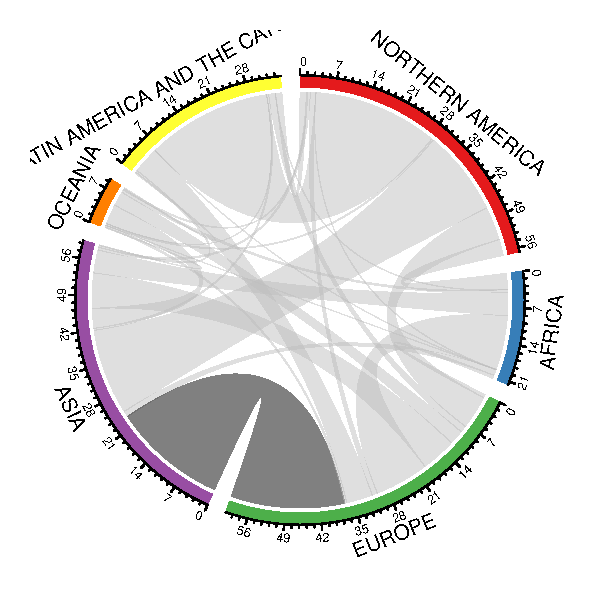
\includegraphics{_main_files/figure-latex/cd-col3-1.pdf}

\begin{Shaded}
\begin{Highlighting}[]
\FunctionTok{chordDiagram}\NormalTok{(}\AttributeTok{x =}\NormalTok{ d, }\AttributeTok{order =}\NormalTok{ r}\SpecialCharTok{$}\NormalTok{reg,}
             \AttributeTok{grid.col =}\NormalTok{ r}\SpecialCharTok{$}\NormalTok{col2, }\AttributeTok{link.visible =}\NormalTok{ d}\SpecialCharTok{$}\NormalTok{show\_link)}
\end{Highlighting}
\end{Shaded}

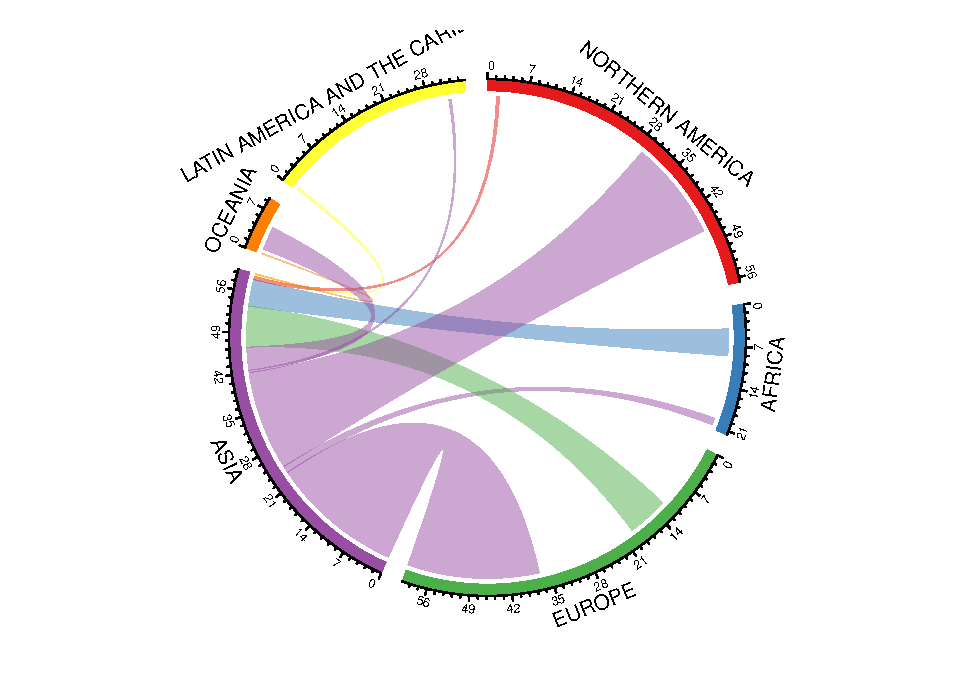
\includegraphics{_main_files/figure-latex/cd-col3-2.pdf}

\hypertarget{chords}{%
\section{Chords}\label{chords}}

\hypertarget{direction}{%
\subsection{Direction}\label{direction}}

\begin{itemize}
\tightlist
\item
  Distinguish direction of bilateral link using

  \begin{itemize}
  \tightlist
  \item
    Different heights at the start and end of the chord links
  \item
    Arrows
  \item
    Combination of both
  \end{itemize}
\item
  Set in \texttt{chordDiagram()} using

  \begin{itemize}
  \tightlist
  \item
    \texttt{directional\ =\ 1} (from link goes from first to second column)
  \item
    \texttt{direction.type} arguments
  \end{itemize}
\end{itemize}

\begin{Shaded}
\begin{Highlighting}[]
\CommentTok{\# drop link\_col column}
\NormalTok{d}\SpecialCharTok{$}\NormalTok{link\_col1 }\OtherTok{\textless{}{-}} \ConstantTok{NULL}

\CommentTok{\# as used by Sander, default of direction.type = "diffHeight"}
\FunctionTok{chordDiagram}\NormalTok{(}\AttributeTok{x =}\NormalTok{ d, }\AttributeTok{order =}\NormalTok{ r}\SpecialCharTok{$}\NormalTok{reg, }\AttributeTok{grid.col =}\NormalTok{ r}\SpecialCharTok{$}\NormalTok{col2, }\AttributeTok{transparency =} \FloatTok{0.25}\NormalTok{,}
             \AttributeTok{directional =} \DecValTok{1}\NormalTok{)}
\end{Highlighting}
\end{Shaded}

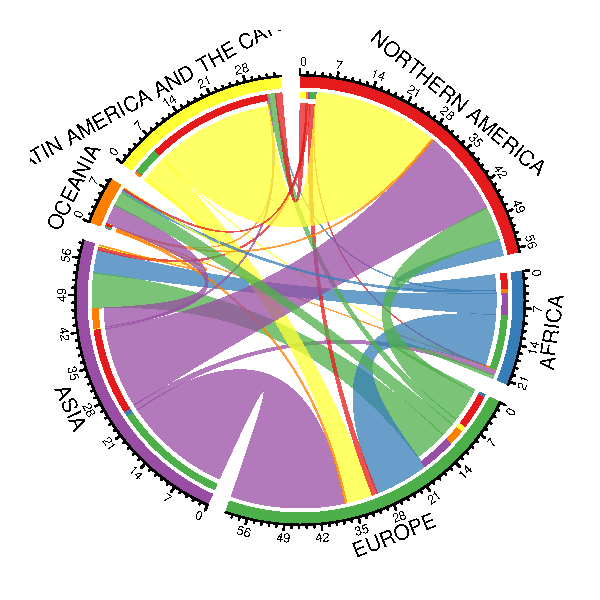
\includegraphics{_main_files/figure-latex/cd-direction1-1.pdf}

\begin{Shaded}
\begin{Highlighting}[]
\CommentTok{\# default arrows are too much}
\FunctionTok{chordDiagram}\NormalTok{(}\AttributeTok{x =}\NormalTok{ d, }\AttributeTok{order =}\NormalTok{ r}\SpecialCharTok{$}\NormalTok{reg, }\AttributeTok{grid.col =}\NormalTok{ r}\SpecialCharTok{$}\NormalTok{col2, }\AttributeTok{transparency =} \FloatTok{0.25}\NormalTok{,}
             \AttributeTok{directional =} \DecValTok{1}\NormalTok{, }\AttributeTok{direction.type =} \FunctionTok{c}\NormalTok{(}\StringTok{"diffHeight"}\NormalTok{, }\StringTok{"arrows"}\NormalTok{))}
\end{Highlighting}
\end{Shaded}

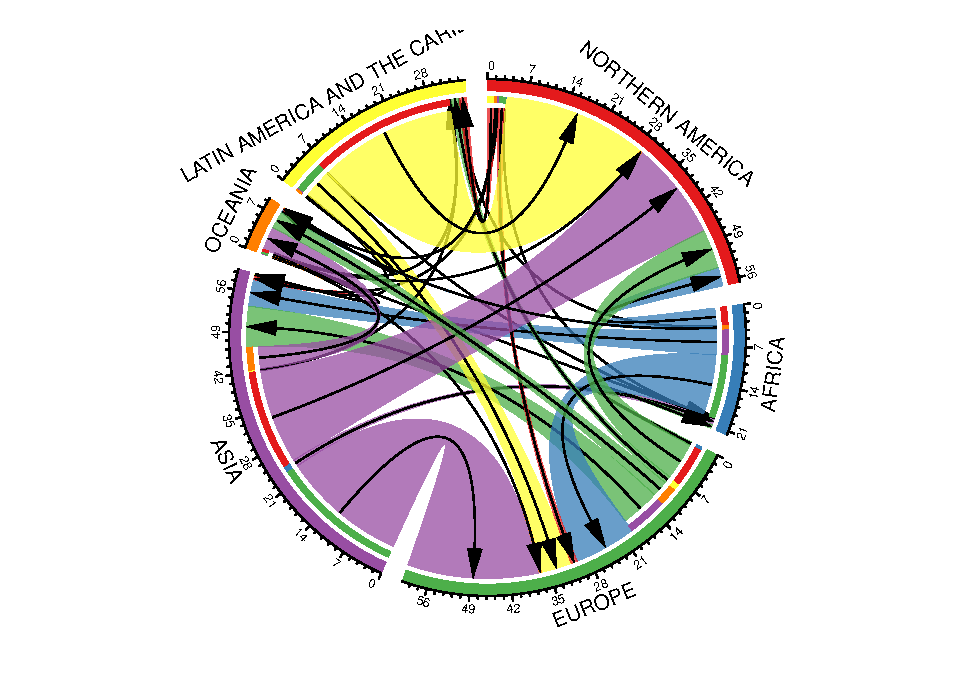
\includegraphics{_main_files/figure-latex/cd-direction1-2.pdf}

\begin{Shaded}
\begin{Highlighting}[]
\CommentTok{\# getting there...}
\FunctionTok{chordDiagram}\NormalTok{(}\AttributeTok{x =}\NormalTok{ d, }\AttributeTok{order =}\NormalTok{ r}\SpecialCharTok{$}\NormalTok{reg, }\AttributeTok{grid.col =}\NormalTok{ r}\SpecialCharTok{$}\NormalTok{col2, }\AttributeTok{transparency =} \FloatTok{0.25}\NormalTok{,}
             \AttributeTok{directional =} \DecValTok{1}\NormalTok{, }\AttributeTok{direction.type =} \FunctionTok{c}\NormalTok{(}\StringTok{"diffHeight"}\NormalTok{, }\StringTok{"arrows"}\NormalTok{),}
             \AttributeTok{link.arr.type =} \StringTok{"big.arrow"}\NormalTok{)}
\end{Highlighting}
\end{Shaded}

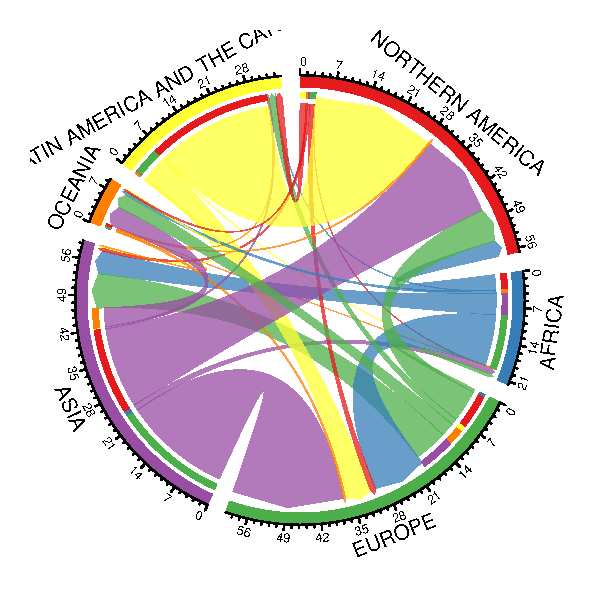
\includegraphics{_main_files/figure-latex/cd-direction1-3.pdf}

\hypertarget{direction-1}{%
\section{Direction}\label{direction-1}}

\begin{itemize}
\tightlist
\item
  Connect the base of the link to the sector through combination of

  \begin{itemize}
  \tightlist
  \item
    Adjusting the difference in height between the beginning and end of chords
  \item
    Removing padding between the axis and the grid (the inner circle where the chords are)
  \end{itemize}
\item
  Set the \texttt{diffHeight} argument to a negative number so that the start of the chord is longer than then end.

  \begin{itemize}
  \tightlist
  \item
    Removes the destination sector bars (chart junk IMO).
  \end{itemize}
\end{itemize}

\begin{Shaded}
\begin{Highlighting}[]
\CommentTok{\# extreme height difference}
\FunctionTok{chordDiagram}\NormalTok{(}\AttributeTok{x =}\NormalTok{ d, }\AttributeTok{order =}\NormalTok{ r}\SpecialCharTok{$}\NormalTok{reg, }\AttributeTok{grid.col =}\NormalTok{ r}\SpecialCharTok{$}\NormalTok{col2, }\AttributeTok{transparency =} \FloatTok{0.25}\NormalTok{,}
             \AttributeTok{directional =} \DecValTok{1}\NormalTok{, }\AttributeTok{direction.type =} \FunctionTok{c}\NormalTok{(}\StringTok{"diffHeight"}\NormalTok{, }\StringTok{"arrows"}\NormalTok{),}
             \AttributeTok{link.arr.type =} \StringTok{"big.arrow"}\NormalTok{, }\AttributeTok{diffHeight  =} \SpecialCharTok{{-}}\FloatTok{0.2}\NormalTok{)}
\end{Highlighting}
\end{Shaded}

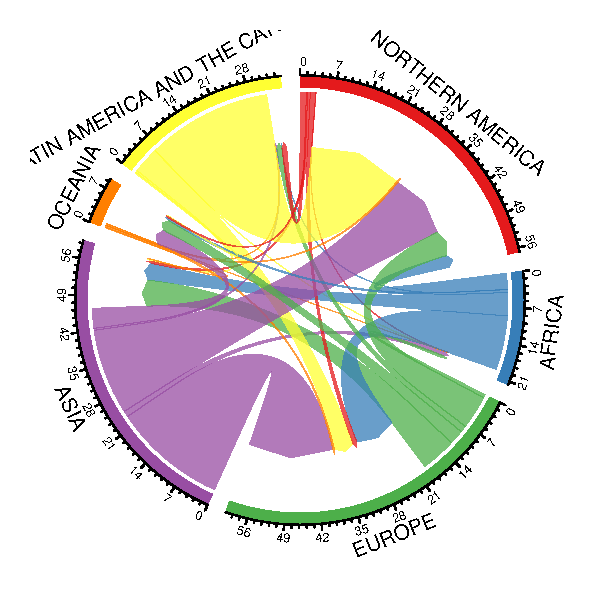
\includegraphics{_main_files/figure-latex/cd-direction2-1.pdf}

\begin{Shaded}
\begin{Highlighting}[]
\CommentTok{\# height difference looks good}
\FunctionTok{chordDiagram}\NormalTok{(}\AttributeTok{x =}\NormalTok{ d, }\AttributeTok{order =}\NormalTok{ r}\SpecialCharTok{$}\NormalTok{reg, }\AttributeTok{grid.col =}\NormalTok{ r}\SpecialCharTok{$}\NormalTok{col2, }\AttributeTok{transparency =} \FloatTok{0.25}\NormalTok{,}
             \AttributeTok{directional =} \DecValTok{1}\NormalTok{, }\AttributeTok{direction.type =} \FunctionTok{c}\NormalTok{(}\StringTok{"diffHeight"}\NormalTok{, }\StringTok{"arrows"}\NormalTok{),}
             \AttributeTok{link.arr.type =} \StringTok{"big.arrow"}\NormalTok{, }\AttributeTok{diffHeight  =} \SpecialCharTok{{-}}\FloatTok{0.05}\NormalTok{)}
\end{Highlighting}
\end{Shaded}

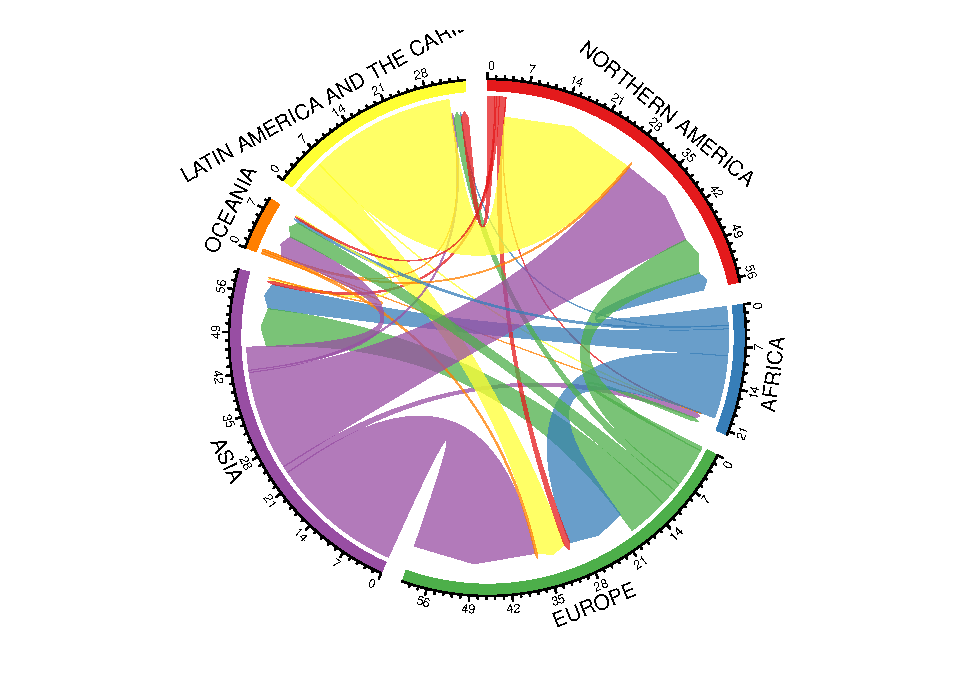
\includegraphics{_main_files/figure-latex/cd-direction2-2.pdf}

\hypertarget{direction-2}{%
\subsection{Direction}\label{direction-2}}

\begin{itemize}
\tightlist
\item
  Set in the \texttt{track.margin} option of \texttt{circos.par()} to remove the padding

  \begin{itemize}
  \tightlist
  \item
    Default of \texttt{track.margin\ =\ c(0.01,\ 0.01)} for chord diagrams - one percent between label names and the axis, and one percent between the axis and the grid (the chords)
  \end{itemize}
\end{itemize}

\begin{Shaded}
\begin{Highlighting}[]
\CommentTok{\# set second margin to zero}
\FunctionTok{circos.par}\NormalTok{(}\AttributeTok{track.margin =} \FunctionTok{c}\NormalTok{(}\FloatTok{0.01}\NormalTok{, }\DecValTok{0}\NormalTok{))}
\FunctionTok{chordDiagram}\NormalTok{(}\AttributeTok{x =}\NormalTok{ d, }\AttributeTok{order =}\NormalTok{ r}\SpecialCharTok{$}\NormalTok{reg, }\AttributeTok{grid.col =}\NormalTok{ r}\SpecialCharTok{$}\NormalTok{col2, }\AttributeTok{transparency =} \FloatTok{0.25}\NormalTok{,}
             \AttributeTok{directional =} \DecValTok{1}\NormalTok{, }\AttributeTok{direction.type =} \FunctionTok{c}\NormalTok{(}\StringTok{"diffHeight"}\NormalTok{, }\StringTok{"arrows"}\NormalTok{),}
             \AttributeTok{link.arr.type =} \StringTok{"big.arrow"}\NormalTok{, }\AttributeTok{diffHeight =} \SpecialCharTok{{-}}\FloatTok{0.05}\NormalTok{)}
\end{Highlighting}
\end{Shaded}

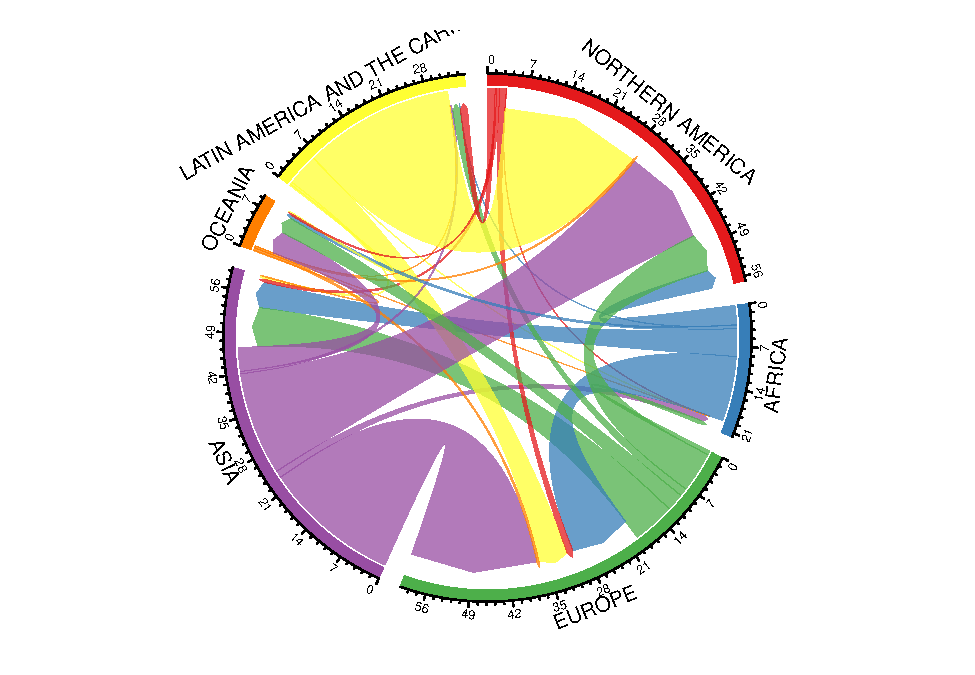
\includegraphics{_main_files/figure-latex/cd-direction3-1.pdf}

\begin{Shaded}
\begin{Highlighting}[]
\CommentTok{\# set second margin to {-}0.01 to get seamless overlap}
\FunctionTok{circos.par}\NormalTok{(}\AttributeTok{track.margin =} \FunctionTok{c}\NormalTok{(}\FloatTok{0.01}\NormalTok{, }\SpecialCharTok{{-}}\FloatTok{0.01}\NormalTok{))}
\FunctionTok{chordDiagram}\NormalTok{(}\AttributeTok{x =}\NormalTok{ d, }\AttributeTok{order =}\NormalTok{ r}\SpecialCharTok{$}\NormalTok{reg, }\AttributeTok{grid.col =}\NormalTok{ r}\SpecialCharTok{$}\NormalTok{col2, }\AttributeTok{transparency =} \FloatTok{0.25}\NormalTok{,}
             \AttributeTok{directional =} \DecValTok{1}\NormalTok{, }\AttributeTok{direction.type =} \FunctionTok{c}\NormalTok{(}\StringTok{"diffHeight"}\NormalTok{, }\StringTok{"arrows"}\NormalTok{),}
             \AttributeTok{link.arr.type =} \StringTok{"big.arrow"}\NormalTok{, }\AttributeTok{diffHeight =} \SpecialCharTok{{-}}\FloatTok{0.05}\NormalTok{)}
\end{Highlighting}
\end{Shaded}

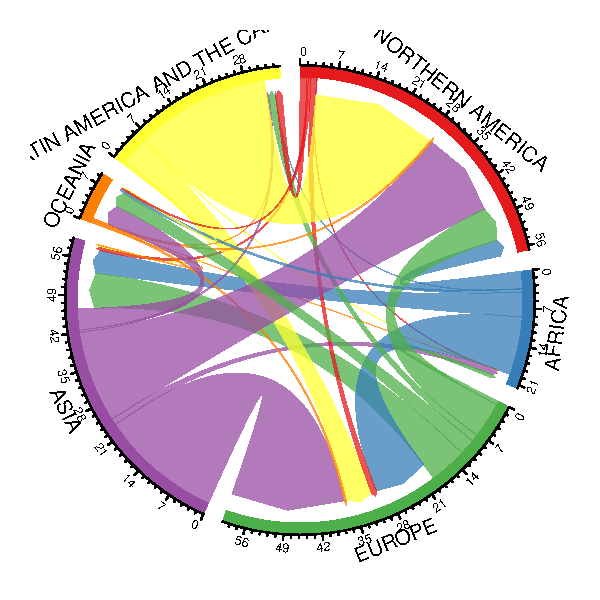
\includegraphics{_main_files/figure-latex/cd-direction3-2.pdf}

\hypertarget{chord-ordering}{%
\subsection{Chord ordering}\label{chord-ordering}}

\begin{itemize}
\tightlist
\item
  Number of options in \texttt{chordDiagram()} to control the chord link order

  \begin{itemize}
  \tightlist
  \item
    \texttt{link.sort} sort the order the links from largest to smaller as the enter and exit the plot, by default \texttt{FALSE}
  \item
    \texttt{link.largest.ontop} sort the order of the plotting of the links so that the smallest are given less prominence. By default \texttt{FALSE}, so plots the links in the last sector last and they appear more predominant
  \end{itemize}
\end{itemize}

\begin{Shaded}
\begin{Highlighting}[]
\CommentTok{\# sort links on sectors}
\FunctionTok{chordDiagram}\NormalTok{(}\AttributeTok{x =}\NormalTok{ d, }\AttributeTok{order =}\NormalTok{ r}\SpecialCharTok{$}\NormalTok{reg, }\AttributeTok{grid.col =}\NormalTok{ r}\SpecialCharTok{$}\NormalTok{col2, }\AttributeTok{transparency =} \FloatTok{0.25}\NormalTok{,}
             \AttributeTok{directional =} \DecValTok{1}\NormalTok{, }\AttributeTok{direction.type =} \FunctionTok{c}\NormalTok{(}\StringTok{"diffHeight"}\NormalTok{, }\StringTok{"arrows"}\NormalTok{),}
             \AttributeTok{link.arr.type =} \StringTok{"big.arrow"}\NormalTok{, }\AttributeTok{diffHeight =} \SpecialCharTok{{-}}\FloatTok{0.05}\NormalTok{,}
             \AttributeTok{link.sort =} \ConstantTok{TRUE}\NormalTok{)}
\end{Highlighting}
\end{Shaded}

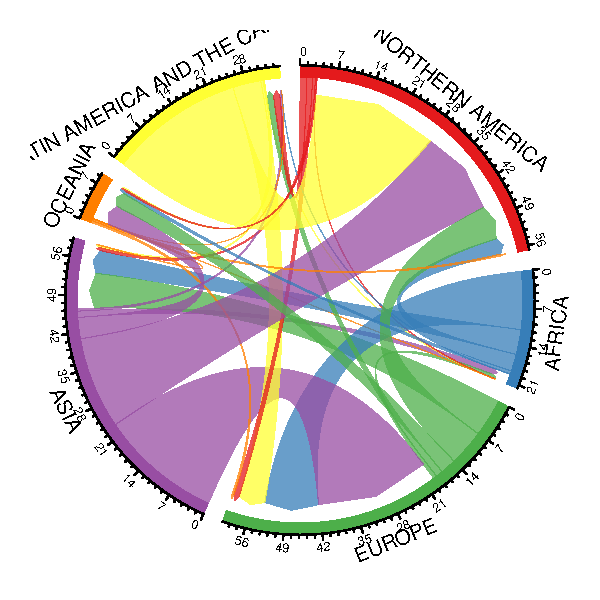
\includegraphics{_main_files/figure-latex/cd-order-1.pdf}

\begin{Shaded}
\begin{Highlighting}[]
\CommentTok{\# sort link plotting order}
\FunctionTok{chordDiagram}\NormalTok{(}\AttributeTok{x =}\NormalTok{ d, }\AttributeTok{order =}\NormalTok{ r}\SpecialCharTok{$}\NormalTok{reg, }\AttributeTok{grid.col =}\NormalTok{ r}\SpecialCharTok{$}\NormalTok{col2, }\AttributeTok{transparency =} \FloatTok{0.25}\NormalTok{,}
             \AttributeTok{directional =} \DecValTok{1}\NormalTok{, }\AttributeTok{direction.type =} \FunctionTok{c}\NormalTok{(}\StringTok{"diffHeight"}\NormalTok{, }\StringTok{"arrows"}\NormalTok{),}
             \AttributeTok{link.arr.type =} \StringTok{"big.arrow"}\NormalTok{, }\AttributeTok{diffHeight =} \SpecialCharTok{{-}}\FloatTok{0.05}\NormalTok{,}
             \AttributeTok{link.sort =} \ConstantTok{TRUE}\NormalTok{, }\AttributeTok{link.largest.ontop =} \ConstantTok{TRUE}\NormalTok{)}
\end{Highlighting}
\end{Shaded}

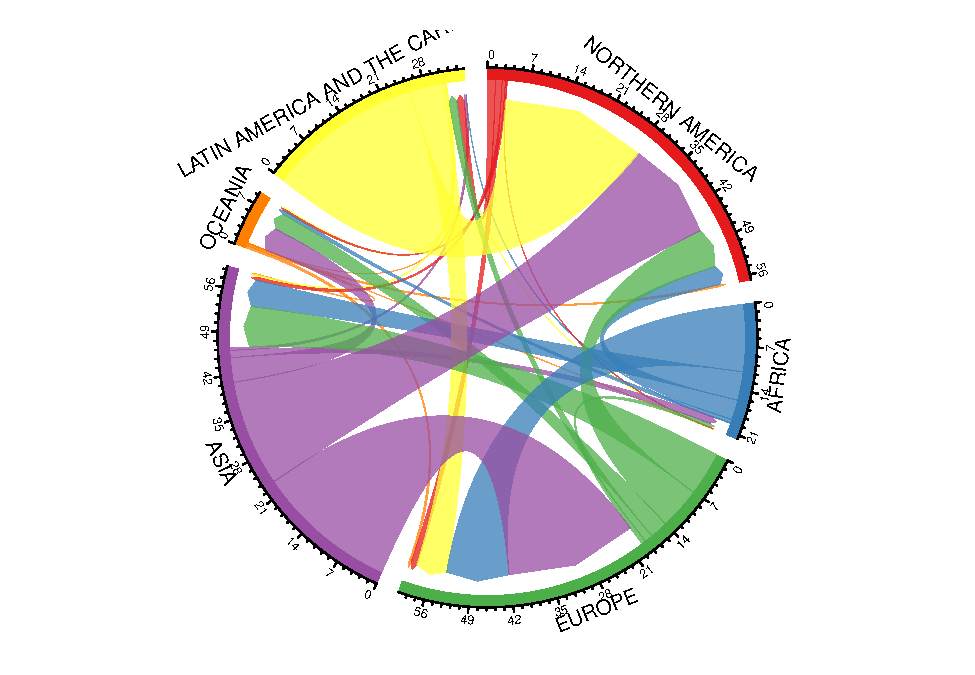
\includegraphics{_main_files/figure-latex/cd-order-2.pdf}

\hypertarget{labels}{%
\section{Labels}\label{labels}}

\hypertarget{labels-1}{%
\subsection{Labels}\label{labels-1}}

\begin{itemize}
\tightlist
\item
  Multiple options for the orientation of labels, set via

  \begin{itemize}
  \tightlist
  \item
    \texttt{inside}, \texttt{outside}, \texttt{clockwise}, \texttt{reverse.clockwise}, \texttt{downward}, \texttt{bending.inside} and \texttt{bending.outside}
  \item
    Cannot pass to \texttt{chordDiagram()} so we have to first use \texttt{annotationTrack} option to only plot the \texttt{grid} (the chords) and \texttt{axis} (default for \texttt{annotationTrack\ =\ c("name",\ "grid",\ "axis")})
  \end{itemize}
\item
  To add the labels we use the \texttt{panel.fun} argument in \texttt{circos.track()}.

  \begin{itemize}
  \tightlist
  \item
    Works like a for loop, cycling through each sector of the track (the circle)
  \item
    For each sector we use \texttt{circos.text()} to add labels at a specified \texttt{x} and \texttt{y} location
  \item
    Can also set the \texttt{facing} orientation of the labels as well as other options such as text size (\texttt{cex}) and colour (\texttt{col})
  \end{itemize}
\end{itemize}

\begin{Shaded}
\begin{Highlighting}[]
\CommentTok{\# drop the name labels}
\FunctionTok{chordDiagram}\NormalTok{(}\AttributeTok{x =}\NormalTok{ d, }\AttributeTok{order =}\NormalTok{ r}\SpecialCharTok{$}\NormalTok{reg, }\AttributeTok{grid.col =}\NormalTok{ r}\SpecialCharTok{$}\NormalTok{col2, }\AttributeTok{transparency =} \FloatTok{0.25}\NormalTok{,}
             \AttributeTok{directional =} \DecValTok{1}\NormalTok{, }\AttributeTok{direction.type =} \FunctionTok{c}\NormalTok{(}\StringTok{"diffHeight"}\NormalTok{, }\StringTok{"arrows"}\NormalTok{),}
             \AttributeTok{link.arr.type =} \StringTok{"big.arrow"}\NormalTok{, }\AttributeTok{diffHeight =} \SpecialCharTok{{-}}\FloatTok{0.05}\NormalTok{,}
             \AttributeTok{link.sort =} \ConstantTok{TRUE}\NormalTok{, }\AttributeTok{link.largest.ontop =} \ConstantTok{TRUE}\NormalTok{,}
             \AttributeTok{annotationTrack =} \FunctionTok{c}\NormalTok{(}\StringTok{"grid"}\NormalTok{, }\StringTok{"axis"}\NormalTok{))}
\end{Highlighting}
\end{Shaded}

\includegraphics{_main_files/figure-latex/cd-label1-1.pdf}

\hypertarget{labels-2}{%
\subsection{Labels}\label{labels-2}}

\begin{itemize}
\tightlist
\item
  No room for labels. We can create this using the \texttt{preAllocateTracks} argument.

  \begin{itemize}
  \tightlist
  \item
    Requires a list of graphical parameters
  \item
    Set \texttt{track.height} as a percentage of plot area.
  \end{itemize}
\end{itemize}

\begin{Shaded}
\begin{Highlighting}[]
\FunctionTok{chordDiagram}\NormalTok{(}\AttributeTok{x =}\NormalTok{ d, }\AttributeTok{order =}\NormalTok{ r}\SpecialCharTok{$}\NormalTok{reg, }\AttributeTok{grid.col =}\NormalTok{ r}\SpecialCharTok{$}\NormalTok{col2, }\AttributeTok{transparency =} \FloatTok{0.25}\NormalTok{,}
             \AttributeTok{directional =} \DecValTok{1}\NormalTok{, }\AttributeTok{direction.type =} \FunctionTok{c}\NormalTok{(}\StringTok{"diffHeight"}\NormalTok{, }\StringTok{"arrows"}\NormalTok{),}
             \AttributeTok{link.arr.type =} \StringTok{"big.arrow"}\NormalTok{, }\AttributeTok{diffHeight =} \SpecialCharTok{{-}}\FloatTok{0.05}\NormalTok{,}
             \AttributeTok{link.sort =} \ConstantTok{TRUE}\NormalTok{, }\AttributeTok{link.largest.ontop =} \ConstantTok{TRUE}\NormalTok{,}
             \AttributeTok{annotationTrack =} \FunctionTok{c}\NormalTok{(}\StringTok{"grid"}\NormalTok{, }\StringTok{"axis"}\NormalTok{),}
             \AttributeTok{preAllocateTracks =} \FunctionTok{list}\NormalTok{(}\AttributeTok{track.height =} \FloatTok{0.1}\NormalTok{))}

\CommentTok{\# add labels}
\FunctionTok{circos.track}\NormalTok{(}\AttributeTok{track.index =} \DecValTok{1}\NormalTok{, }\AttributeTok{bg.border =} \ConstantTok{NA}\NormalTok{, }\AttributeTok{panel.fun =} \ControlFlowTok{function}\NormalTok{(x, y) \{}
  \CommentTok{\# create temporary objects for the sector name and x{-}limits}
\NormalTok{  reg\_lab }\OtherTok{\textless{}{-}} \FunctionTok{get.cell.meta.data}\NormalTok{(}\StringTok{"sector.index"}\NormalTok{)}
\NormalTok{  xx }\OtherTok{\textless{}{-}} \FunctionTok{get.cell.meta.data}\NormalTok{(}\StringTok{"xlim"}\NormalTok{)}
  \CommentTok{\# use the temporary objects to add text in each sector of the track}
  \FunctionTok{circos.text}\NormalTok{(}\AttributeTok{x =} \FunctionTok{mean}\NormalTok{(xx), }\AttributeTok{y =} \DecValTok{1}\NormalTok{, }\AttributeTok{labels =}\NormalTok{ reg\_lab, }\AttributeTok{facing =} \StringTok{"bending"}\NormalTok{)}
\NormalTok{\})}
\end{Highlighting}
\end{Shaded}

\includegraphics{_main_files/figure-latex/cd-label2-1.pdf}

\hypertarget{labels-3}{%
\subsection{Labels}\label{labels-3}}

\begin{itemize}
\tightlist
\item
  Still not enough room for longer labels.

  \begin{itemize}
  \tightlist
  \item
    Increase the \texttt{track.height}
  \item
    Create two labels for some regions
  \item
    Reduce the font size using \texttt{cex} in \texttt{circos.text()} - default is \texttt{cex\ =\ 1}
  \end{itemize}
\end{itemize}

\begin{Shaded}
\begin{Highlighting}[]
\FunctionTok{str\_wrap}\NormalTok{(}\AttributeTok{string =}\NormalTok{ r}\SpecialCharTok{$}\NormalTok{reg, }\AttributeTok{width =} \DecValTok{14}\NormalTok{)}
\end{Highlighting}
\end{Shaded}

\begin{verbatim}
## [1] "NORTHERN\nAMERICA"                 "AFRICA"                           
## [3] "EUROPE"                            "ASIA"                             
## [5] "OCEANIA"                           "LATIN AMERICA\nAND THE\nCARIBBEAN"
\end{verbatim}

\begin{Shaded}
\begin{Highlighting}[]
\NormalTok{r }\OtherTok{\textless{}{-}}\NormalTok{ r }\SpecialCharTok{\%\textgreater{}\%}
  \CommentTok{\# title case for labels}
  \FunctionTok{mutate}\NormalTok{(}\AttributeTok{lab =} \FunctionTok{str\_to\_title}\NormalTok{(}\AttributeTok{string =}\NormalTok{ reg),}
         \AttributeTok{lab =} \FunctionTok{str\_replace}\NormalTok{(}\AttributeTok{string =}\NormalTok{ lab, }\AttributeTok{pattern =} \StringTok{"And The"}\NormalTok{, }\AttributeTok{replacement =} \StringTok{"\&"}\NormalTok{),}
  \CommentTok{\# use str\_wrap to split longer labels into two}
         \AttributeTok{lab =} \FunctionTok{str\_wrap}\NormalTok{(}\AttributeTok{string =}\NormalTok{ lab, }\AttributeTok{width =} \DecValTok{14}\NormalTok{)) }\SpecialCharTok{\%\textgreater{}\%}
  \CommentTok{\# separate based on \textbackslash{}n}
  \FunctionTok{separate}\NormalTok{(}\AttributeTok{col =}\NormalTok{ lab, }\AttributeTok{into =} \FunctionTok{c}\NormalTok{(}\StringTok{"lab1"}\NormalTok{, }\StringTok{"lab2"}\NormalTok{), }\AttributeTok{sep =} \StringTok{"}\SpecialCharTok{\textbackslash{}n}\StringTok{"}\NormalTok{, }\AttributeTok{fill =} \StringTok{"right"}\NormalTok{) }\SpecialCharTok{\%\textgreater{}\%}
  \CommentTok{\# positioning for first lab1, needs to be further out if lab2 exists}
  \FunctionTok{mutate}\NormalTok{(}\AttributeTok{y =} \FunctionTok{ifelse}\NormalTok{(}\AttributeTok{test =} \SpecialCharTok{!}\FunctionTok{is.na}\NormalTok{(lab2), }\AttributeTok{yes =} \DecValTok{1}\NormalTok{, }\AttributeTok{no =} \FloatTok{0.8}\NormalTok{))}
\end{Highlighting}
\end{Shaded}

\hypertarget{labels-4}{%
\subsection{Labels}\label{labels-4}}

\begin{itemize}
\tightlist
\item
  Still not enough room for longer labels.

  \begin{itemize}
  \tightlist
  \item
    Increase the \texttt{track.height}
  \item
    Create two labels for some regions
  \item
    Reduce the font size using \texttt{cex} in \texttt{circos.text()} - default is \texttt{cex\ =\ 1}
  \end{itemize}
\end{itemize}

\begin{Shaded}
\begin{Highlighting}[]
\NormalTok{r}
\end{Highlighting}
\end{Shaded}

\begin{verbatim}
## # A tibble: 6 x 8
##   reg                             reg_order col1   col2  col3  lab1  lab2      y
##   <chr>                               <dbl> <chr>  <chr> <chr> <chr> <chr> <dbl>
## 1 NORTHERN AMERICA                        1 black  #E41~ Red   Nort~ Amer~   1  
## 2 AFRICA                                  2 gold   #377~ Grey  Afri~ <NA>    0.8
## 3 EUROPE                                  3 orange #4DA~ Grey  Euro~ <NA>    0.8
## 4 ASIA                                    4 blue   #984~ Grey  Asia  <NA>    0.8
## 5 OCEANIA                                 5 purple #FF7~ Grey  Ocea~ <NA>    0.8
## 6 LATIN AMERICA AND THE CARIBBEAN         6 red    #FFF~ Grey  Lati~ & Ca~   1
\end{verbatim}

\hypertarget{labels-5}{%
\subsection{Labels}\label{labels-5}}

\begin{Shaded}
\begin{Highlighting}[]
\FunctionTok{chordDiagram}\NormalTok{(}\AttributeTok{x =}\NormalTok{ d, }\AttributeTok{order =}\NormalTok{ r}\SpecialCharTok{$}\NormalTok{reg, }\AttributeTok{grid.col =}\NormalTok{ r}\SpecialCharTok{$}\NormalTok{col2, }\AttributeTok{transparency =} \FloatTok{0.25}\NormalTok{,}
             \AttributeTok{directional =} \DecValTok{1}\NormalTok{, }\AttributeTok{direction.type =} \FunctionTok{c}\NormalTok{(}\StringTok{"diffHeight"}\NormalTok{, }\StringTok{"arrows"}\NormalTok{),}
             \AttributeTok{link.arr.type =} \StringTok{"big.arrow"}\NormalTok{, }\AttributeTok{diffHeight =} \SpecialCharTok{{-}}\FloatTok{0.05}\NormalTok{,}
             \AttributeTok{link.sort =} \ConstantTok{TRUE}\NormalTok{, }\AttributeTok{link.largest.ontop =} \ConstantTok{TRUE}\NormalTok{,}
             \AttributeTok{annotationTrack =} \FunctionTok{c}\NormalTok{(}\StringTok{"grid"}\NormalTok{, }\StringTok{"axis"}\NormalTok{),}
             \CommentTok{\# increase to 0.2 to fit two lines of labels}
             \AttributeTok{preAllocateTracks =} \FunctionTok{list}\NormalTok{(}\AttributeTok{track.height =} \FloatTok{0.2}\NormalTok{))}

\FunctionTok{circos.track}\NormalTok{(}\AttributeTok{track.index =} \DecValTok{1}\NormalTok{, }\AttributeTok{bg.border =} \ConstantTok{NA}\NormalTok{, }\AttributeTok{panel.fun =} \ControlFlowTok{function}\NormalTok{(x, y) \{}
\NormalTok{  s }\OtherTok{\textless{}{-}} \FunctionTok{get.cell.meta.data}\NormalTok{(}\StringTok{"sector.index"}\NormalTok{)}
  \CommentTok{\# filter to row of r for the sector\textquotesingle{}s region to create a temporary rr}
\NormalTok{  rr }\OtherTok{\textless{}{-}} \FunctionTok{filter}\NormalTok{(r, reg }\SpecialCharTok{==}\NormalTok{ s)}
\NormalTok{  xx }\OtherTok{\textless{}{-}} \FunctionTok{get.cell.meta.data}\NormalTok{(}\StringTok{"xlim"}\NormalTok{)}
  \CommentTok{\# use temporary rr to add text}
  \FunctionTok{circos.text}\NormalTok{(}\AttributeTok{x =} \FunctionTok{mean}\NormalTok{(xx), }\AttributeTok{y =}\NormalTok{ rr}\SpecialCharTok{$}\NormalTok{y, }\AttributeTok{labels =}\NormalTok{ rr}\SpecialCharTok{$}\NormalTok{lab1, }\AttributeTok{facing =} \StringTok{"bending"}\NormalTok{,}
              \AttributeTok{cex =} \FloatTok{0.8}\NormalTok{)}
  \FunctionTok{circos.text}\NormalTok{(}\AttributeTok{x =} \FunctionTok{mean}\NormalTok{(xx), }\AttributeTok{y =} \FloatTok{0.6}\NormalTok{,  }\AttributeTok{labels =}\NormalTok{ rr}\SpecialCharTok{$}\NormalTok{lab2, }\AttributeTok{facing =} \StringTok{"bending"}\NormalTok{,}
              \AttributeTok{cex =} \FloatTok{0.8}\NormalTok{)}
\NormalTok{\})}
\end{Highlighting}
\end{Shaded}

\includegraphics{_main_files/figure-latex/cd-label4-1.pdf}

\hypertarget{saving}{%
\subsection{Saving}\label{saving}}

\begin{itemize}
\tightlist
\item
  Always save as PDF to give scalable image

  \begin{itemize}
  \tightlist
  \item
    We can zoom in very closely and we will still see the chords
  \item
    If we save a vector graphic, e.g.~PNG these details will disappear.
  \end{itemize}
\item
  Use the \texttt{pdf()} function before the plot to open a PDF
\item
  Use \texttt{dev.off()} after the plot code to close the PDF
\end{itemize}

\begin{Shaded}
\begin{Highlighting}[]
\FunctionTok{pdf}\NormalTok{(}\AttributeTok{file =} \StringTok{"./plot/un\_stock\_2019.pdf"}\NormalTok{, }\AttributeTok{width =} \DecValTok{4}\NormalTok{, }\AttributeTok{height =} \DecValTok{4}\NormalTok{)}

\FunctionTok{circos.par}\NormalTok{(}\AttributeTok{track.margin =} \FunctionTok{c}\NormalTok{(}\FloatTok{0.01}\NormalTok{, }\SpecialCharTok{{-}}\FloatTok{0.01}\NormalTok{), }\AttributeTok{gap.degree =} \DecValTok{5}\NormalTok{, }\AttributeTok{start.degree =} \DecValTok{90}\NormalTok{)}
\FunctionTok{chordDiagram}\NormalTok{(}\AttributeTok{x =}\NormalTok{ d, }\AttributeTok{order =}\NormalTok{ r}\SpecialCharTok{$}\NormalTok{reg, }\AttributeTok{grid.col =}\NormalTok{ r}\SpecialCharTok{$}\NormalTok{col2, }\AttributeTok{transparency =} \FloatTok{0.25}\NormalTok{,}
             \AttributeTok{directional =} \DecValTok{1}\NormalTok{, }\AttributeTok{direction.type =} \FunctionTok{c}\NormalTok{(}\StringTok{"diffHeight"}\NormalTok{, }\StringTok{"arrows"}\NormalTok{),}
             \AttributeTok{link.arr.type =} \StringTok{"big.arrow"}\NormalTok{, }\AttributeTok{diffHeight =} \SpecialCharTok{{-}}\FloatTok{0.05}\NormalTok{,}
             \AttributeTok{link.sort =} \ConstantTok{TRUE}\NormalTok{, }\AttributeTok{link.largest.ontop =} \ConstantTok{TRUE}\NormalTok{,}
             \AttributeTok{annotationTrack =} \FunctionTok{c}\NormalTok{(}\StringTok{"grid"}\NormalTok{, }\StringTok{"axis"}\NormalTok{),}
             \AttributeTok{preAllocateTracks =} \FunctionTok{list}\NormalTok{(}\AttributeTok{track.height =} \FloatTok{0.2}\NormalTok{))}
\FunctionTok{circos.track}\NormalTok{(}\AttributeTok{track.index =} \DecValTok{1}\NormalTok{, }\AttributeTok{bg.border =} \ConstantTok{NA}\NormalTok{, }\AttributeTok{panel.fun =} \ControlFlowTok{function}\NormalTok{(x, y) \{}
\NormalTok{  s }\OtherTok{\textless{}{-}} \FunctionTok{get.cell.meta.data}\NormalTok{(}\StringTok{"sector.index"}\NormalTok{)}
\NormalTok{  rr }\OtherTok{\textless{}{-}} \FunctionTok{filter}\NormalTok{(r, reg }\SpecialCharTok{==}\NormalTok{ s)}
\NormalTok{  xx }\OtherTok{\textless{}{-}} \FunctionTok{get.cell.meta.data}\NormalTok{(}\StringTok{"xlim"}\NormalTok{)}
  \FunctionTok{circos.text}\NormalTok{(}\AttributeTok{x =} \FunctionTok{mean}\NormalTok{(xx), }\AttributeTok{y =}\NormalTok{ rr}\SpecialCharTok{$}\NormalTok{y, }\AttributeTok{labels =}\NormalTok{ rr}\SpecialCharTok{$}\NormalTok{lab1, }\AttributeTok{facing =} \StringTok{"bending"}\NormalTok{, }\AttributeTok{cex =} \FloatTok{0.8}\NormalTok{)}
  \FunctionTok{circos.text}\NormalTok{(}\AttributeTok{x =} \FunctionTok{mean}\NormalTok{(xx), }\AttributeTok{y =} \FloatTok{0.6}\NormalTok{,  }\AttributeTok{labels =}\NormalTok{ rr}\SpecialCharTok{$}\NormalTok{lab2, }\AttributeTok{facing =} \StringTok{"bending"}\NormalTok{, }\AttributeTok{cex =} \FloatTok{0.8}\NormalTok{)}
\NormalTok{\})}

\FunctionTok{dev.off}\NormalTok{()}
\end{Highlighting}
\end{Shaded}

\hypertarget{saving-1}{%
\subsection{Saving}\label{saving-1}}

\begin{itemize}
\tightlist
\item
  Left: PNG with \texttt{width\ =\ 4,\ height\ =\ 4}
\item
  Right: PDF with \texttt{width\ =\ 4,\ height\ =\ 4}
\end{itemize}

\includegraphics[width=0.45\linewidth]{plot/un_stock_2019}
\includegraphics[width=0.45\linewidth]{plot/un_stock_2019}

\begin{itemize}
\tightlist
\item
  Could increase resolution of PNG with larger dimensions but at the cost of very large file sizes
\end{itemize}

\hypertarget{exercise-ex8.r}{%
\subsection{Exercise (ex8.R)}\label{exercise-ex8.r}}

\begin{Shaded}
\begin{Highlighting}[]
\CommentTok{\# 0.  a) Load the KOSTAT2021.Rproj file. }
\CommentTok{\#     Run the getwd() below. It should print the directory where the }
\CommentTok{\#     KOSTAT2021.Rproj file is located.}
\FunctionTok{getwd}\NormalTok{()}
\CommentTok{\#     b) Load the packages used in this exercise}
\FunctionTok{library}\NormalTok{(tidyverse)}
\FunctionTok{library}\NormalTok{(migest)}
\FunctionTok{library}\NormalTok{(circlize)}
\DocumentationTok{\#\#}
\DocumentationTok{\#\#}
\DocumentationTok{\#\#}
\CommentTok{\# 1. Run the code below to read in the label data in korea\_cd\_labels.csv taken}
\CommentTok{\#    from https://www.tandfonline.com/doi/full/10.1080/21681376.2018.1431149 }
\NormalTok{r }\OtherTok{\textless{}{-}} \FunctionTok{read\_csv}\NormalTok{(}\StringTok{"./data/korea\_cd\_labels.csv"}\NormalTok{) }
\FunctionTok{View}\NormalTok{(r)}
\CommentTok{\# 2. Run the code below to select the 2020 Korean internal migration data, }
\CommentTok{\#    for plotting, excluding within region movements}
\NormalTok{d }\OtherTok{\textless{}{-}}\NormalTok{ korea\_reg }\SpecialCharTok{\%\textgreater{}\%}
  \FunctionTok{filter}\NormalTok{(year }\SpecialCharTok{==} \DecValTok{2020}\NormalTok{, }
\NormalTok{         orig }\SpecialCharTok{!=}\NormalTok{ dest)}
\NormalTok{d}
\CommentTok{\# 3. Run the code below to check that all the regions in the object r are in the }
\CommentTok{\#    migration data frame d}
\FunctionTok{setdiff}\NormalTok{(}\AttributeTok{x =} \FunctionTok{union}\NormalTok{(d}\SpecialCharTok{$}\NormalTok{orig, d}\SpecialCharTok{$}\NormalTok{dest), }\AttributeTok{y =}\NormalTok{ r}\SpecialCharTok{$}\NormalTok{region)}
\CommentTok{\# 4. Modify d to enable a more sensible plot}
\CommentTok{\#    1) divide flow column by a thousand}
\CommentTok{\#    2) adjust the data frame to the three relevant columns for chordDiagram()}
\NormalTok{d }\OtherTok{\textless{}{-}}\NormalTok{ d }\SpecialCharTok{\%\textgreater{}\%}
  \FunctionTok{select}\NormalTok{(}\SpecialCharTok{{-}}\DocumentationTok{\#\#\#\#\#) \%\textgreater{}\%}
  \FunctionTok{mutate}\NormalTok{(}\AttributeTok{flow =}\NormalTok{ flow}\SpecialCharTok{/}\DocumentationTok{\#\#\#\#\#)}
\CommentTok{\# 5. Check the data is in the correct by format by plotting a chord diagram }
\CommentTok{\#    using the default settings}
\FunctionTok{chordDiagram}\NormalTok{(}\AttributeTok{x =} \DocumentationTok{\#\#\#\#\#)}
\CommentTok{\# 6. Plot a chord diagram using }
\CommentTok{\#    a. the order of provinces from r}
\CommentTok{\#    b. colours from the col column in r}
\CommentTok{\#    c. transparency set to 0.25}
\FunctionTok{chordDiagram}\NormalTok{(}\AttributeTok{x =}\NormalTok{ d, }\AttributeTok{order =} \DocumentationTok{\#\#\#\#\#$region, grid.col = r$\#\#\#\#\#, \#\#\#\#\# = 0.25)}
\CommentTok{\# 7. Edit the code below to }
\CommentTok{\#    a. add directional arrows }
\CommentTok{\#    b. change the height at the start and end of the chords to {-}0.04 }
\FunctionTok{chordDiagram}\NormalTok{(}\AttributeTok{x =}\NormalTok{ d, }\AttributeTok{order =}\NormalTok{ r}\SpecialCharTok{$}\DocumentationTok{\#\#\#\#\#, grid.col = r$col, transparency = 0.25,}
             \AttributeTok{directional =} \DocumentationTok{\#\#\#\#\#, direction.type = c(\#\#\#\#\#, "arrows"),}
             \DocumentationTok{\#\#\#\#\# = "big.arrow", diffHeight = \#\#\#\#\#)}
\CommentTok{\# 8. Use the circos.par function to set}
\CommentTok{\#    a. track margins to c(0.01, {-}0.01)}
\CommentTok{\#    d. start degree to 90}
\CommentTok{\#    c. gap degree to a the gap column in object r}
\CommentTok{\#    d. plot a chord diagram with these setting based based on the code in the }
\CommentTok{\#       answer above}
\FunctionTok{circos.par}\NormalTok{(}\AttributeTok{track.margin =} \FunctionTok{c}\NormalTok{(}\DocumentationTok{\#\#\#\#\#, {-}0.01), \#\#\#\#\# = 90, gap.degree = r$\#\#\#\#\#)}
\FunctionTok{chordDiagram}\NormalTok{(}\AttributeTok{x =}\NormalTok{ d, }\AttributeTok{order =}\NormalTok{ r}\SpecialCharTok{$}\NormalTok{region, }\AttributeTok{grid.col =}\NormalTok{ r}\SpecialCharTok{$}\NormalTok{col, }\AttributeTok{transparency =} \FloatTok{0.25}\NormalTok{,}
             \AttributeTok{directional =} \DecValTok{1}\NormalTok{, }\AttributeTok{direction.type =} \FunctionTok{c}\NormalTok{(}\StringTok{"diffHeight"}\NormalTok{, }\StringTok{"arrows"}\NormalTok{),}
             \AttributeTok{link.arr.type =} \StringTok{"big.arrow"}\NormalTok{, }\AttributeTok{diffHeight =} \SpecialCharTok{{-}}\FloatTok{0.04}\NormalTok{)}
\CommentTok{\# 9. Edit below to sort the chord links }
\CommentTok{\#    a. into and out of each section}
\CommentTok{\#    b. largest links on top}
\FunctionTok{chordDiagram}\NormalTok{(}\AttributeTok{x =}\NormalTok{ d, }\AttributeTok{order =}\NormalTok{ r}\SpecialCharTok{$}\NormalTok{region, }\AttributeTok{grid.col =}\NormalTok{ r}\SpecialCharTok{$}\NormalTok{col, }\AttributeTok{transparency =} \FloatTok{0.25}\NormalTok{,}
             \AttributeTok{directional =} \DecValTok{1}\NormalTok{, }\AttributeTok{direction.type =} \FunctionTok{c}\NormalTok{(}\StringTok{"diffHeight"}\NormalTok{, }\StringTok{"arrows"}\NormalTok{),}
             \AttributeTok{link.arr.type =} \StringTok{"big.arrow"}\NormalTok{, }\AttributeTok{diffHeight =} \SpecialCharTok{{-}}\FloatTok{0.04}\NormalTok{, }
             \AttributeTok{link.sort =} \DocumentationTok{\#\#\#\#\#, link.largest.ontop = \#\#\#\#\#)}
\CommentTok{\# 10. Edit the code below to}
\CommentTok{\#     a. plot only the grid and the axis}
\CommentTok{\#     b. set the track height of the label area to 0.1}
\FunctionTok{chordDiagram}\NormalTok{(}\AttributeTok{x =}\NormalTok{ d, }\AttributeTok{order =}\NormalTok{ r}\SpecialCharTok{$}\NormalTok{region, }\AttributeTok{grid.col =}\NormalTok{ r}\SpecialCharTok{$}\NormalTok{col, }\AttributeTok{transparency =} \FloatTok{0.25}\NormalTok{,}
             \AttributeTok{directional =} \DecValTok{1}\NormalTok{, }\AttributeTok{direction.type =} \FunctionTok{c}\NormalTok{(}\StringTok{"diffHeight"}\NormalTok{, }\StringTok{"arrows"}\NormalTok{),}
             \AttributeTok{link.arr.type =} \StringTok{"big.arrow"}\NormalTok{, }\AttributeTok{diffHeight =} \SpecialCharTok{{-}}\FloatTok{0.04}\NormalTok{, }
             \AttributeTok{link.sort =} \ConstantTok{TRUE}\NormalTok{, }\AttributeTok{link.largest.ontop =} \ConstantTok{TRUE}\NormalTok{, }
             \DocumentationTok{\#\#\#\#\# = c("grid", \#\#\#\#\#),}
             \AttributeTok{preAllocateTracks =} \FunctionTok{list}\NormalTok{(}\AttributeTok{track.height =} \DocumentationTok{\#\#\#\#\#))}
\CommentTok{\# 11. Add the labels in the track by}
\CommentTok{\#     a. setting y position of label to 1}
\CommentTok{\#     b. setting text facing to bending}
\CommentTok{\#     c. setting the font size to 0.7}
\FunctionTok{circos.track}\NormalTok{(}\AttributeTok{track.index =} \DecValTok{1}\NormalTok{, }\AttributeTok{bg.border =} \ConstantTok{NA}\NormalTok{, }\AttributeTok{panel.fun =} \ControlFlowTok{function}\NormalTok{(x, y) \{}
\NormalTok{  s }\OtherTok{=} \FunctionTok{get.cell.meta.data}\NormalTok{(}\StringTok{"sector.index"}\NormalTok{)}
\NormalTok{  xx }\OtherTok{=} \FunctionTok{get.cell.meta.data}\NormalTok{(}\StringTok{"xlim"}\NormalTok{)}
\NormalTok{  rr }\OtherTok{=} \FunctionTok{filter}\NormalTok{(}\DocumentationTok{\#\#\#\#\#, region == s)}
  \FunctionTok{circos.text}\NormalTok{(}\AttributeTok{x =} \FunctionTok{mean}\NormalTok{(xx), }\AttributeTok{y =} \DocumentationTok{\#\#\#\#\#, labels = rr$label\_en, }
              \AttributeTok{facing =} \DocumentationTok{\#\#\#\#\#, \#\#\#\#\# = 0.7)}
\ErrorTok{\}}\NormalTok{)}
\CommentTok{\# 12. Use the code in question 10 and 11 to create the PDF version of the plot }
\FunctionTok{pdf}\NormalTok{(}\AttributeTok{file =} \StringTok{"./exercise/korea2020\_en.pdf"}\NormalTok{, }\AttributeTok{width =} \DecValTok{5}\NormalTok{, }\AttributeTok{height =} \DecValTok{5}\NormalTok{)}





\DocumentationTok{\#\#\#\#\# paste in here ...}







\FunctionTok{dev.off}\NormalTok{()}
\CommentTok{\# 13. Run the code below to check the PDF (might not work on Mac {-} if so, }
\CommentTok{\#     manually open PDF file to view)}
\FunctionTok{file.show}\NormalTok{(}\StringTok{"./exercise/korea2020\_en.pdf"}\NormalTok{)}
\CommentTok{\# 14. Complete the code below to add a second set of Korean labels.}
\CommentTok{\#     Note: East Asian characters require a non{-}standard font families {-} see }
\CommentTok{\#           ?pdfFonts for options. Might not require to set family depending on}
\CommentTok{\#           settings in your computer and/or RStudio}
\FunctionTok{pdf}\NormalTok{(}\AttributeTok{file =} \StringTok{"./exercise/korea2020.pdf"}\NormalTok{, }\AttributeTok{width =} \DecValTok{5}\NormalTok{, }\AttributeTok{height =} \DecValTok{5}\NormalTok{, }\AttributeTok{family =} \StringTok{"Korea1"}\NormalTok{)}
\FunctionTok{chordDiagram}\NormalTok{(}\AttributeTok{x =}\NormalTok{ d, }\AttributeTok{order =}\NormalTok{ r}\SpecialCharTok{$}\NormalTok{region, }\AttributeTok{grid.col =}\NormalTok{ r}\SpecialCharTok{$}\NormalTok{col, }\AttributeTok{transparency =} \FloatTok{0.25}\NormalTok{,}
             \AttributeTok{directional =} \DecValTok{1}\NormalTok{, }\AttributeTok{direction.type =} \FunctionTok{c}\NormalTok{(}\StringTok{"diffHeight"}\NormalTok{, }\StringTok{"arrows"}\NormalTok{),}
             \AttributeTok{link.arr.type =} \StringTok{"big.arrow"}\NormalTok{, }\AttributeTok{diffHeight =} \SpecialCharTok{{-}}\FloatTok{0.04}\NormalTok{, }
             \AttributeTok{link.sort =} \ConstantTok{TRUE}\NormalTok{, }\AttributeTok{link.largest.ontop =} \ConstantTok{TRUE}\NormalTok{, }
             \AttributeTok{annotationTrack =} \FunctionTok{c}\NormalTok{(}\StringTok{"grid"}\NormalTok{, }\StringTok{"axis"}\NormalTok{),}
             \AttributeTok{preAllocateTracks =} \FunctionTok{list}\NormalTok{(}\AttributeTok{track.height =} \FloatTok{0.1}\NormalTok{))}
\FunctionTok{circos.track}\NormalTok{(}\AttributeTok{track.index =} \DecValTok{1}\NormalTok{, }\AttributeTok{bg.border =} \ConstantTok{NA}\NormalTok{, }\AttributeTok{panel.fun =} \ControlFlowTok{function}\NormalTok{(x, y) \{}
\NormalTok{  s }\OtherTok{=} \FunctionTok{get.cell.meta.data}\NormalTok{(}\StringTok{"sector.index"}\NormalTok{)}
  \DocumentationTok{\#\#\#\#\# \textless{}{-} filter(r, region == s)}
\NormalTok{  xx }\OtherTok{=} \FunctionTok{get.cell.meta.data}\NormalTok{(}\StringTok{"xlim"}\NormalTok{)}
  \FunctionTok{circos.text}\NormalTok{(}\AttributeTok{x =} \FunctionTok{mean}\NormalTok{(xx), }\AttributeTok{y =} \FloatTok{1.5}\NormalTok{, }\AttributeTok{labels =}\NormalTok{ rr}\SpecialCharTok{$}\NormalTok{label\_en, }
              \AttributeTok{facing =} \StringTok{"bending"}\NormalTok{, }\AttributeTok{cex =} \FloatTok{0.7}\NormalTok{)}
  \FunctionTok{circos.text}\NormalTok{(}\AttributeTok{x =} \FunctionTok{mean}\NormalTok{(xx), }\AttributeTok{y =} \FloatTok{0.9}\NormalTok{, }\AttributeTok{labels =}\NormalTok{ rr}\SpecialCharTok{$}\DocumentationTok{\#\#\#\#\#, }
              \AttributeTok{facing =} \StringTok{"bending"}\NormalTok{, }\AttributeTok{cex =} \FloatTok{0.7}\NormalTok{)}
\NormalTok{\})}
\FunctionTok{dev.off}\NormalTok{()}
\FunctionTok{file.show}\NormalTok{(}\StringTok{"./exercise/korea2020.pdf"}\NormalTok{)}
\CommentTok{\# 15. Run the code below to check the PDF (might not work on Mac {-} if so, }
\CommentTok{\#     manually open PDF file to view)}
\FunctionTok{file.show}\NormalTok{(}\StringTok{"./exercise/korea2020.pdf"}\NormalTok{)}
\end{Highlighting}
\end{Shaded}

\hypertarget{sankey-plots-for-visualising-bilateral-migration}{%
\chapter{Sankey Plots for Visualising Bilateral Migration}\label{sankey-plots-for-visualising-bilateral-migration}}

\hypertarget{background-4}{%
\section{Background}\label{background-4}}

\hypertarget{background-5}{%
\subsection{Background}\label{background-5}}

\begin{itemize}
\tightlist
\item
  An alternative approach to visualize bilateral migration are Sankey or alluvial plots.
\item
  Sankey plots feature arrows with width proportional to the flow quantity.
\item
  Named after Irish Captain Sankey, who used to show the energy efficiency of a steam engine in 1898.
\item
  Minard's plot of Napoleon's Russian Campaign of 1812 was made in 1869 - before Sankey
\item
  Alluvial plots are a form of Sankey plot

  \begin{itemize}
  \tightlist
  \item
    Contain blocks at nodes (e.g.~origin and destination of migraiton flows)
  \item
    No space between blocks, implying a meaningful axis, unlike Sankey plots that do have spaces
  \end{itemize}
\end{itemize}

\hypertarget{men-in-napoleons-1812-russian-campaign}{%
\subsection{Men in Napoleon's 1812 Russian Campaign}\label{men-in-napoleons-1812-russian-campaign}}

\includegraphics[width=27.82in]{img/Minard-napolean}

\hypertarget{sankey-plot-of-migration-in-nature-by-butler2017}{%
\subsection{\texorpdfstring{Sankey plot of migration in Nature by \citet{Butler2017}}{Sankey plot of migration in Nature by @Butler2017}}\label{sankey-plot-of-migration-in-nature-by-butler2017}}

\includegraphics{img/Migration_Graphic.pdf}

\hypertarget{sankey-plots-in-r}{%
\subsection{Sankey plots in R}\label{sankey-plots-in-r}}

\begin{itemize}
\tightlist
\item
  As the number of regions or countries increases the plot become more cumbersome

  \begin{itemize}
  \tightlist
  \item
    Labels for the smaller areas get too small and the plotting area becomes a very long rectangle making it awkward to fit on paper or view on the screen.
  \item
    In such cases I prefer chord diagrams
  \end{itemize}
\item
  There are a few packages in R that have functions for Sankey plots, such as \emph{sankey}, \emph{PantaRhei}, \emph{networkD3}, \emph{sankeywheel}, \emph{plotly}, \emph{ggsankey}.

  \begin{itemize}
  \tightlist
  \item
    Also \emph{ggalluvial} which produces an allivual plot, but without any spaces between each sectors.
  \end{itemize}
\item
  I am going to use \emph{ggforce} which I think is the most flexible

  \begin{itemize}
  \tightlist
  \item
    At the cost of a new layout for the data set
  \item
    Good labels need a some work - as in \emph{circlize} -
    because Sankey plots tend to have many set axis
  \item
    Migration data tend to have only two set axis (origin and destinations)
  \end{itemize}
\end{itemize}

\hypertarget{sankey-plots-in-r-1}{%
\subsection{Sankey plots in R}\label{sankey-plots-in-r-1}}

\begin{itemize}
\tightlist
\item
  For Sankey plots with \emph{ggforce} the \texttt{gather\_set\_data()} function formats the data so that every migration corridor has two rows for the size of the migration at the origin and destination
\item
  Can then use standard \texttt{ggplot()} function to set up the plot format. The mapping argument includes

  \begin{itemize}
  \tightlist
  \item
    \texttt{id} the id of the ribbons
  \item
    \texttt{value} the size of the ribbons
  \item
    \texttt{split} categories for splitting of the ribbons
  \end{itemize}
\item
  Add on layers for the ribbons themselves using \texttt{geom\_parallel\_sets()}
\item
  Add blocks at the end of the ribbons to allow for clear identification of origin and destinations using \texttt{geom\_parallel\_sets\_axes()}
\item
  Add labels at the start and end of the ribbons using \texttt{geom\_parallel\_sets\_axes()}
\end{itemize}

\hypertarget{data-format}{%
\section{Data Format}\label{data-format}}

\hypertarget{un-international-migrant-stock-data-2020-3}{%
\subsection{UN international migrant stock data 2020}\label{un-international-migrant-stock-data-2020-3}}

\begin{itemize}
\tightlist
\item
  \citet{UNPD2020} stock data as before
\end{itemize}

\begin{Shaded}
\begin{Highlighting}[]
\FunctionTok{library}\NormalTok{(tidyverse)}
\NormalTok{un }\OtherTok{\textless{}{-}} \FunctionTok{read\_csv}\NormalTok{(}\AttributeTok{file =} \StringTok{"data/un\_desa\_ims\_tidy.csv"}\NormalTok{)}
\NormalTok{un}
\end{Highlighting}
\end{Shaded}

\begin{verbatim}
## # A tibble: 259,357 x 6
##     year     stock por_name por_code pob_name           pob_code
##    <dbl>     <dbl> <chr>       <dbl> <chr>                 <dbl>
##  1  1990 152986157 WORLD         900 WORLD                   900
##  2  1995 161289976 WORLD         900 WORLD                   900
##  3  2000 173230585 WORLD         900 WORLD                   900
##  4  2005 191446828 WORLD         900 WORLD                   900
##  5  2010 220983187 WORLD         900 WORLD                   900
##  6  2015 247958644 WORLD         900 WORLD                   900
##  7  2020 280598105 WORLD         900 WORLD                   900
##  8  1990  15334807 WORLD         900 Sub-Saharan Africa      947
##  9  1995  16488973 WORLD         900 Sub-Saharan Africa      947
## 10  2000  15638014 WORLD         900 Sub-Saharan Africa      947
## # ... with 259,347 more rows
\end{verbatim}

\hypertarget{un-international-migrant-stock-data-2020-4}{%
\subsection{UN international migrant stock data 2020}\label{un-international-migrant-stock-data-2020-4}}

\begin{itemize}
\tightlist
\item
  Plot between World Bank income groups
\end{itemize}

\begin{Shaded}
\begin{Highlighting}[]
\CommentTok{\# codes for income groups}
\NormalTok{cc }\OtherTok{\textless{}{-}} \FunctionTok{c}\NormalTok{(}\DecValTok{1503}\SpecialCharTok{:}\DecValTok{1500}\NormalTok{, }\DecValTok{2003}\NormalTok{)}
\NormalTok{d }\OtherTok{\textless{}{-}}\NormalTok{ un }\SpecialCharTok{\%\textgreater{}\%}
  \FunctionTok{filter}\NormalTok{(por\_code }\SpecialCharTok{\%in\%}\NormalTok{ cc, }
\NormalTok{         pob\_code }\SpecialCharTok{\%in\%}\NormalTok{ cc,}
\NormalTok{         year }\SpecialCharTok{==} \DecValTok{2020}\NormalTok{) }\SpecialCharTok{\%\textgreater{}\%}
  \FunctionTok{rename}\NormalTok{(}\AttributeTok{orig =}\NormalTok{ pob\_name, }
         \AttributeTok{dest =}\NormalTok{ por\_name) }\SpecialCharTok{\%\textgreater{}\%}
  \FunctionTok{mutate}\NormalTok{(}\AttributeTok{stock =}\NormalTok{ stock}\SpecialCharTok{/}\FloatTok{1e6}\NormalTok{)}
\NormalTok{d}
\end{Highlighting}
\end{Shaded}

\begin{verbatim}
## # A tibble: 16 x 6
##     year  stock dest                          por_code orig             pob_code
##    <dbl>  <dbl> <chr>                            <dbl> <chr>               <dbl>
##  1  2020 45.8   High-income countries             1503 High-income cou~     1503
##  2  2020 59.9   High-income countries             1503 Upper-middle-in~     1502
##  3  2020 58.0   High-income countries             1503 Lower-middle-in~     1501
##  4  2020 10.5   High-income countries             1503 Low-income coun~     1500
##  5  2020  5.66  Upper-middle-income countries     1502 High-income cou~     1503
##  6  2020 20.6   Upper-middle-income countries     1502 Upper-middle-in~     1502
##  7  2020 18.3   Upper-middle-income countries     1502 Lower-middle-in~     1501
##  8  2020 10.8   Upper-middle-income countries     1502 Low-income coun~     1500
##  9  2020  0.961 Lower-middle-income countries     1501 High-income cou~     1503
## 10  2020  6.45  Lower-middle-income countries     1501 Upper-middle-in~     1502
## 11  2020 10.5   Lower-middle-income countries     1501 Lower-middle-in~     1501
## 12  2020  7.93  Lower-middle-income countries     1501 Low-income coun~     1500
## 13  2020  0.102 Low-income countries              1500 High-income cou~     1503
## 14  2020  0.579 Low-income countries              1500 Upper-middle-in~     1502
## 15  2020  2.90  Low-income countries              1500 Lower-middle-in~     1501
## 16  2020  8.12  Low-income countries              1500 Low-income coun~     1500
\end{verbatim}

\hypertarget{data-format-1}{%
\subsection{Data format}\label{data-format-1}}

\begin{itemize}
\tightlist
\item
  Format data for Sankey plot using \texttt{gather\_set\_data()} function in \emph{ggforce}
\end{itemize}

\begin{Shaded}
\begin{Highlighting}[]
\FunctionTok{library}\NormalTok{(ggforce)}

\NormalTok{s }\OtherTok{\textless{}{-}}\NormalTok{ d }\SpecialCharTok{\%\textgreater{}\%}
  \FunctionTok{select}\NormalTok{(orig, dest, stock) }\SpecialCharTok{\%\textgreater{}\%}
  \FunctionTok{gather\_set\_data}\NormalTok{(}\AttributeTok{x =} \DecValTok{1}\SpecialCharTok{:}\DecValTok{2}\NormalTok{)}
\NormalTok{s}
\end{Highlighting}
\end{Shaded}

\begin{verbatim}
## # A tibble: 32 x 6
##    orig                          dest            stock    id x     y            
##    <chr>                         <chr>           <dbl> <int> <chr> <chr>        
##  1 High-income countries         High-income c~ 45.8       1 orig  High-income ~
##  2 Upper-middle-income countries High-income c~ 59.9       2 orig  Upper-middle~
##  3 Lower-middle-income countries High-income c~ 58.0       3 orig  Lower-middle~
##  4 Low-income countries          High-income c~ 10.5       4 orig  Low-income c~
##  5 High-income countries         Upper-middle-~  5.66      5 orig  High-income ~
##  6 Upper-middle-income countries Upper-middle-~ 20.6       6 orig  Upper-middle~
##  7 Lower-middle-income countries Upper-middle-~ 18.3       7 orig  Lower-middle~
##  8 Low-income countries          Upper-middle-~ 10.8       8 orig  Low-income c~
##  9 High-income countries         Lower-middle-~  0.961     9 orig  High-income ~
## 10 Upper-middle-income countries Lower-middle-~  6.45     10 orig  Upper-middle~
## # ... with 22 more rows
\end{verbatim}

\hypertarget{data-format-2}{%
\subsection{Data format}\label{data-format-2}}

\begin{Shaded}
\begin{Highlighting}[]
\FunctionTok{tail}\NormalTok{(s)}
\end{Highlighting}
\end{Shaded}

\begin{verbatim}
## # A tibble: 6 x 6
##   orig                          dest            stock    id x     y             
##   <chr>                         <chr>           <dbl> <int> <chr> <chr>         
## 1 Lower-middle-income countries Lower-middle-~ 10.5      11 dest  Lower-middle-~
## 2 Low-income countries          Lower-middle-~  7.93     12 dest  Lower-middle-~
## 3 High-income countries         Low-income co~  0.102    13 dest  Low-income co~
## 4 Upper-middle-income countries Low-income co~  0.579    14 dest  Low-income co~
## 5 Lower-middle-income countries Low-income co~  2.90     15 dest  Low-income co~
## 6 Low-income countries          Low-income co~  8.12     16 dest  Low-income co~
\end{verbatim}

\hypertarget{parrellel-sets}{%
\section{Parrellel Sets}\label{parrellel-sets}}

\hypertarget{default-plot}{%
\subsection{Default Plot}\label{default-plot}}

\begin{itemize}
\tightlist
\item
  Pass the different columns to \texttt{ggplot()} mappings
\item
  The \texttt{geom\_parallel\_sets()} plots the ribbons
\end{itemize}

\begin{Shaded}
\begin{Highlighting}[]
\FunctionTok{ggplot}\NormalTok{(}\AttributeTok{data =}\NormalTok{ s,}
       \AttributeTok{mapping =} \FunctionTok{aes}\NormalTok{(}\AttributeTok{x =}\NormalTok{ x, }\AttributeTok{id =}\NormalTok{ id, }\AttributeTok{value =}\NormalTok{ stock, }\AttributeTok{split =}\NormalTok{ y)) }\SpecialCharTok{+}
  \FunctionTok{geom\_parallel\_sets}\NormalTok{()}
\end{Highlighting}
\end{Shaded}

\includegraphics{_main_files/figure-latex/sankey-default-1.pdf}

\hypertarget{default-plot-1}{%
\subsection{Default Plot}\label{default-plot-1}}

\begin{itemize}
\tightlist
\item
  By default the x-axis goes in alphabetical order

  \begin{itemize}
  \tightlist
  \item
    Use factors to set ordering of categorical variable
  \end{itemize}
\end{itemize}

\begin{Shaded}
\begin{Highlighting}[]
\FunctionTok{levels}\NormalTok{(s}\SpecialCharTok{$}\NormalTok{x)}
\end{Highlighting}
\end{Shaded}

\begin{verbatim}
## NULL
\end{verbatim}

\begin{Shaded}
\begin{Highlighting}[]
\NormalTok{s }\OtherTok{\textless{}{-}} \FunctionTok{mutate}\NormalTok{(s, }\AttributeTok{x =} \FunctionTok{fct\_rev}\NormalTok{(x))}
\FunctionTok{levels}\NormalTok{(s}\SpecialCharTok{$}\NormalTok{x)}
\end{Highlighting}
\end{Shaded}

\begin{verbatim}
## [1] "orig" "dest"
\end{verbatim}

\begin{Shaded}
\begin{Highlighting}[]
\FunctionTok{ggplot}\NormalTok{(}\AttributeTok{data =}\NormalTok{ s,}
       \AttributeTok{mapping =} \FunctionTok{aes}\NormalTok{(}\AttributeTok{x =}\NormalTok{ x, }\AttributeTok{id =}\NormalTok{ id, }\AttributeTok{value =}\NormalTok{ stock, }\AttributeTok{split =}\NormalTok{ y)) }\SpecialCharTok{+}
  \FunctionTok{geom\_parallel\_sets}\NormalTok{()}
\end{Highlighting}
\end{Shaded}

\includegraphics{_main_files/figure-latex/sankey-x-axis-1.pdf}

\hypertarget{set-axes}{%
\section{Set Axes}\label{set-axes}}

\hypertarget{set-axes-1}{%
\subsection{Set Axes}\label{set-axes-1}}

\begin{itemize}
\tightlist
\item
  The \texttt{geom\_parallel\_sets\_axes()} function adds blocks besides the start and end of the ribbons

  \begin{itemize}
  \tightlist
  \item
    Set the width (as a proportion) using \texttt{axis.width}
  \end{itemize}
\end{itemize}

\begin{Shaded}
\begin{Highlighting}[]
\CommentTok{\# default axis.width}
\FunctionTok{ggplot}\NormalTok{(}\AttributeTok{data =}\NormalTok{ s,}
       \AttributeTok{mapping =} \FunctionTok{aes}\NormalTok{(}\AttributeTok{x =}\NormalTok{ x, }\AttributeTok{id =}\NormalTok{ id, }\AttributeTok{value =}\NormalTok{ stock, }\AttributeTok{split =}\NormalTok{ y)) }\SpecialCharTok{+}
  \FunctionTok{geom\_parallel\_sets}\NormalTok{() }\SpecialCharTok{+}
  \FunctionTok{geom\_parallel\_sets\_axes}\NormalTok{()}
\end{Highlighting}
\end{Shaded}

\includegraphics{_main_files/figure-latex/sankey-set-axis-1.pdf}

\begin{Shaded}
\begin{Highlighting}[]
\CommentTok{\# wider axis.width}
\FunctionTok{ggplot}\NormalTok{(}\AttributeTok{data =}\NormalTok{ s,}
      \AttributeTok{mapping =} \FunctionTok{aes}\NormalTok{(}\AttributeTok{x =}\NormalTok{ x, }\AttributeTok{id =}\NormalTok{ id, }\AttributeTok{value =}\NormalTok{ stock, }\AttributeTok{split =}\NormalTok{ y)) }\SpecialCharTok{+}
  \FunctionTok{geom\_parallel\_sets}\NormalTok{() }\SpecialCharTok{+}
  \FunctionTok{geom\_parallel\_sets\_axes}\NormalTok{(}\AttributeTok{axis.width =} \FloatTok{0.1}\NormalTok{)}
\end{Highlighting}
\end{Shaded}

\includegraphics{_main_files/figure-latex/sankey-set-axis-2.pdf}

\hypertarget{colour-1}{%
\section{Colour}\label{colour-1}}

\hypertarget{colour-2}{%
\subsection{Colour}\label{colour-2}}

\begin{itemize}
\tightlist
\item
  Use \texttt{mapping} in \texttt{geom\_parallel\_sets()} to set the colours

  \begin{itemize}
  \tightlist
  \item
    Fill the colours following the origin regions, as was the case in the chord diagrams
  \end{itemize}
\item
  The \texttt{geom\_parallel\_sets\_axes()} cannot take a fill colour from the data frame
\end{itemize}

\begin{Shaded}
\begin{Highlighting}[]
\CommentTok{\# geom\_parallel\_sets\_axes cannot take fill colours from data}
\FunctionTok{ggplot}\NormalTok{(}\AttributeTok{data =}\NormalTok{ s, }\AttributeTok{mapping =} \FunctionTok{aes}\NormalTok{(}\AttributeTok{x =}\NormalTok{ x, }\AttributeTok{id =}\NormalTok{ id, }\AttributeTok{value =}\NormalTok{ stock, }\AttributeTok{split =}\NormalTok{ y, }\AttributeTok{fill =}\NormalTok{ orig)) }\SpecialCharTok{+}
  \FunctionTok{geom\_parallel\_sets}\NormalTok{() }\SpecialCharTok{+}
  \FunctionTok{geom\_parallel\_sets\_axes}\NormalTok{()}
\end{Highlighting}
\end{Shaded}

\begin{verbatim}
## Warning: Computation failed in `stat_parallel_sets_axes()`:
## Axis aesthetics must be constant in each split
\end{verbatim}

\includegraphics{_main_files/figure-latex/sankey-col-1.pdf}

\begin{Shaded}
\begin{Highlighting}[]
\CommentTok{\# set fill colour for parallel\_sets only}
\FunctionTok{ggplot}\NormalTok{(}\AttributeTok{data =}\NormalTok{ s, }\AttributeTok{mapping =} \FunctionTok{aes}\NormalTok{(}\AttributeTok{x =}\NormalTok{ x, }\AttributeTok{id =}\NormalTok{ id, }\AttributeTok{value =}\NormalTok{ stock, }\AttributeTok{split =}\NormalTok{ y)) }\SpecialCharTok{+}
  \FunctionTok{geom\_parallel\_sets}\NormalTok{(}\AttributeTok{mapping =} \FunctionTok{aes}\NormalTok{(}\AttributeTok{fill =}\NormalTok{ orig)) }\SpecialCharTok{+}
  \FunctionTok{geom\_parallel\_sets\_axes}\NormalTok{()}
\end{Highlighting}
\end{Shaded}

\includegraphics{_main_files/figure-latex/sankey-col-2.pdf}

\hypertarget{ribbon-colour---failed-axis-colour}{%
\subsection{Ribbon colour - failed axis colour}\label{ribbon-colour---failed-axis-colour}}

\hypertarget{ribbon-transparency}{%
\subsection{Ribbon transparency}\label{ribbon-transparency}}

\begin{itemize}
\tightlist
\item
  Add some transparency in the ribbons using the \texttt{alpha} argument in \texttt{geom\_parallel\_sets()}
\end{itemize}

\begin{Shaded}
\begin{Highlighting}[]
\CommentTok{\# transparency of 0.8}
\FunctionTok{ggplot}\NormalTok{(}\AttributeTok{data =}\NormalTok{ s, }\AttributeTok{mapping =} \FunctionTok{aes}\NormalTok{(}\AttributeTok{x =}\NormalTok{ x, }\AttributeTok{id =}\NormalTok{ id, }\AttributeTok{value =}\NormalTok{ stock, }\AttributeTok{split =}\NormalTok{ y)) }\SpecialCharTok{+}
  \FunctionTok{geom\_parallel\_sets}\NormalTok{(}\AttributeTok{mapping =} \FunctionTok{aes}\NormalTok{(}\AttributeTok{fill =}\NormalTok{ orig), }\AttributeTok{alpha =} \FloatTok{0.8}\NormalTok{) }\SpecialCharTok{+}
  \FunctionTok{geom\_parallel\_sets\_axes}\NormalTok{()}
\end{Highlighting}
\end{Shaded}

\includegraphics{_main_files/figure-latex/sankey-col-tran-1.pdf}

\begin{Shaded}
\begin{Highlighting}[]
\CommentTok{\# transparency of 0.2}
\FunctionTok{ggplot}\NormalTok{(}\AttributeTok{data =}\NormalTok{ s, }\AttributeTok{mapping =} \FunctionTok{aes}\NormalTok{(}\AttributeTok{x =}\NormalTok{ x, }\AttributeTok{id =}\NormalTok{ id, }\AttributeTok{value =}\NormalTok{ stock, }\AttributeTok{split =}\NormalTok{ y)) }\SpecialCharTok{+}
  \FunctionTok{geom\_parallel\_sets}\NormalTok{(}\AttributeTok{mapping =} \FunctionTok{aes}\NormalTok{(}\AttributeTok{fill =}\NormalTok{ orig), }\AttributeTok{alpha =} \FloatTok{0.2}\NormalTok{) }\SpecialCharTok{+}
  \FunctionTok{geom\_parallel\_sets\_axes}\NormalTok{()}
\end{Highlighting}
\end{Shaded}

\includegraphics{_main_files/figure-latex/sankey-col-tran-2.pdf}

\hypertarget{axis-colour}{%
\subsection{Axis colour}\label{axis-colour}}

\begin{itemize}
\tightlist
\item
  To see the set axis colours we can draw an outline using the \texttt{colour} argument.

  \begin{itemize}
  \tightlist
  \item
    Also set \texttt{fill\ =\ "transparent"} in order to view the underlying ribbons
  \end{itemize}
\end{itemize}

\begin{Shaded}
\begin{Highlighting}[]
\CommentTok{\# geom\_parallel\_sets\_axes is an axis, can provide outline colour only}
\FunctionTok{ggplot}\NormalTok{(}\AttributeTok{data =}\NormalTok{ s, }\AttributeTok{mapping =} \FunctionTok{aes}\NormalTok{(}\AttributeTok{x =}\NormalTok{ x, }\AttributeTok{id =}\NormalTok{ id, }\AttributeTok{value =}\NormalTok{ stock, }\AttributeTok{split =}\NormalTok{ y)) }\SpecialCharTok{+}
  \FunctionTok{geom\_parallel\_sets}\NormalTok{(}\AttributeTok{mapping =} \FunctionTok{aes}\NormalTok{(}\AttributeTok{fill =}\NormalTok{ orig), }\AttributeTok{alpha =} \FloatTok{0.8}\NormalTok{) }\SpecialCharTok{+}
  \FunctionTok{geom\_parallel\_sets\_axes}\NormalTok{(}\AttributeTok{colour =} \StringTok{"black"}\NormalTok{)}
\end{Highlighting}
\end{Shaded}

\includegraphics{_main_files/figure-latex/sankey-axis-col-1.pdf}

\begin{Shaded}
\begin{Highlighting}[]
\CommentTok{\# geom\_parallel\_sets\_axes is an axis, can provide outline colour only}
\FunctionTok{ggplot}\NormalTok{(}\AttributeTok{data =}\NormalTok{ s, }\AttributeTok{mapping =} \FunctionTok{aes}\NormalTok{(}\AttributeTok{x =}\NormalTok{ x, }\AttributeTok{id =}\NormalTok{ id, }\AttributeTok{value =}\NormalTok{ stock, }\AttributeTok{split =}\NormalTok{ y)) }\SpecialCharTok{+}
  \FunctionTok{geom\_parallel\_sets}\NormalTok{(}\AttributeTok{mapping =} \FunctionTok{aes}\NormalTok{(}\AttributeTok{fill =}\NormalTok{ orig)) }\SpecialCharTok{+}
  \FunctionTok{geom\_parallel\_sets\_axes}\NormalTok{(}\AttributeTok{fill =} \StringTok{"transparent"}\NormalTok{, }\AttributeTok{colour =} \StringTok{"black"}\NormalTok{, }
                            \AttributeTok{axis.width =} \FloatTok{0.1}\NormalTok{)}
\end{Highlighting}
\end{Shaded}

\includegraphics{_main_files/figure-latex/sankey-axis-col-2.pdf}

\hypertarget{axis-colour-1}{%
\subsection{Axis colour}\label{axis-colour-1}}

\begin{itemize}
\tightlist
\item
  Tweak the width in \texttt{geom\_parallel\_sets()} so that it fills into the axis box

  \begin{itemize}
  \tightlist
  \item
    Need to set \texttt{fill\ =\ "transparent"}
  \end{itemize}
\end{itemize}

\begin{Shaded}
\begin{Highlighting}[]
\FunctionTok{ggplot}\NormalTok{(}\AttributeTok{data =}\NormalTok{ s, }\AttributeTok{mapping =} \FunctionTok{aes}\NormalTok{(}\AttributeTok{x =}\NormalTok{ x, }\AttributeTok{id =}\NormalTok{ id, }\AttributeTok{value =}\NormalTok{ stock, }\AttributeTok{split =}\NormalTok{ y)) }\SpecialCharTok{+}
  \FunctionTok{geom\_parallel\_sets}\NormalTok{(}\AttributeTok{mapping =} \FunctionTok{aes}\NormalTok{(}\AttributeTok{fill =}\NormalTok{ orig), }\AttributeTok{alpha =} \FloatTok{0.8}\NormalTok{, }\AttributeTok{axis.width =} \SpecialCharTok{{-}}\FloatTok{0.1}\NormalTok{) }\SpecialCharTok{+}
  \FunctionTok{geom\_parallel\_sets\_axes}\NormalTok{(}\AttributeTok{fill =} \StringTok{"transparent"}\NormalTok{, }\AttributeTok{colour =} \StringTok{"black"}\NormalTok{, }
                          \AttributeTok{axis.width =} \FloatTok{0.1}\NormalTok{)}
\end{Highlighting}
\end{Shaded}

\includegraphics{_main_files/figure-latex/sankey-axis-fill-1.pdf}

\begin{Shaded}
\begin{Highlighting}[]
\CommentTok{\# narrower set axes}
\FunctionTok{ggplot}\NormalTok{(}\AttributeTok{data =}\NormalTok{ s,}\AttributeTok{mapping =} \FunctionTok{aes}\NormalTok{(}\AttributeTok{x =}\NormalTok{ x, }\AttributeTok{id =}\NormalTok{ id, }\AttributeTok{value =}\NormalTok{ stock, }\AttributeTok{split =}\NormalTok{ y)) }\SpecialCharTok{+}
  \FunctionTok{geom\_parallel\_sets}\NormalTok{(}\AttributeTok{mapping =} \FunctionTok{aes}\NormalTok{(}\AttributeTok{fill =}\NormalTok{ orig), }\AttributeTok{alpha =} \FloatTok{0.8}\NormalTok{, }\AttributeTok{axis.width =} \SpecialCharTok{{-}}\FloatTok{0.05}\NormalTok{) }\SpecialCharTok{+}
  \FunctionTok{geom\_parallel\_sets\_axes}\NormalTok{(}\AttributeTok{fill =} \StringTok{"transparent"}\NormalTok{, }\AttributeTok{colour =} \StringTok{"black"}\NormalTok{, }
                          \AttributeTok{axis.width =} \FloatTok{0.05}\NormalTok{)}
\end{Highlighting}
\end{Shaded}

\includegraphics{_main_files/figure-latex/sankey-axis-fill-2.pdf}

\hypertarget{labels-6}{%
\section{Labels}\label{labels-6}}

\hypertarget{labels-7}{%
\subsection{Labels}\label{labels-7}}

\begin{itemize}
\tightlist
\item
  Add labels on the x-axis using \texttt{scale\_x\_discrete()} from \emph{ggplot2}
\item
  Add labels to the sets using \texttt{geom\_parallel\_sets\_labels()} from \emph{ggforce}

  \begin{itemize}
  \tightlist
  \item
    Terrible default positions and angles if labels are not very short.
  \end{itemize}
\end{itemize}

\begin{Shaded}
\begin{Highlighting}[]
\FunctionTok{ggplot}\NormalTok{(}\AttributeTok{data =}\NormalTok{ s, }\AttributeTok{mapping =} \FunctionTok{aes}\NormalTok{(}\AttributeTok{x =}\NormalTok{ x, }\AttributeTok{id =}\NormalTok{ id, }\AttributeTok{value =}\NormalTok{ stock, }\AttributeTok{split =}\NormalTok{ y)) }\SpecialCharTok{+}
  \FunctionTok{geom\_parallel\_sets}\NormalTok{(}\AttributeTok{mapping =} \FunctionTok{aes}\NormalTok{(}\AttributeTok{fill =}\NormalTok{ orig), }\AttributeTok{alpha =} \FloatTok{0.8}\NormalTok{, }\AttributeTok{axis.width =} \SpecialCharTok{{-}}\FloatTok{0.05}\NormalTok{) }\SpecialCharTok{+}
  \FunctionTok{geom\_parallel\_sets\_axes}\NormalTok{(}\AttributeTok{fill =} \StringTok{"transparent"}\NormalTok{, }\AttributeTok{colour =} \StringTok{"black"}\NormalTok{, }
                          \AttributeTok{axis.width =} \FloatTok{0.05}\NormalTok{) }\SpecialCharTok{+}
  \FunctionTok{guides}\NormalTok{(}\AttributeTok{fill =} \StringTok{"none"}\NormalTok{) }\SpecialCharTok{+}
  \FunctionTok{geom\_parallel\_sets\_labels}\NormalTok{() }\SpecialCharTok{+}
  \FunctionTok{scale\_x\_discrete}\NormalTok{(}\AttributeTok{labels =} \FunctionTok{c}\NormalTok{(}\AttributeTok{orig =} \StringTok{"Place of Birth"}\NormalTok{, }
                              \AttributeTok{dest =} \StringTok{"Place of Residence"}\NormalTok{))}
\end{Highlighting}
\end{Shaded}

\includegraphics{_main_files/figure-latex/sankey-default-lab-1.pdf}

\begin{Shaded}
\begin{Highlighting}[]
\FunctionTok{ggplot}\NormalTok{(}\AttributeTok{data =}\NormalTok{ s, }\AttributeTok{mapping =} \FunctionTok{aes}\NormalTok{(}\AttributeTok{x =}\NormalTok{ x, }\AttributeTok{id =}\NormalTok{ id, }\AttributeTok{value =}\NormalTok{ stock, }\AttributeTok{split =}\NormalTok{ y)) }\SpecialCharTok{+}
  \FunctionTok{geom\_parallel\_sets}\NormalTok{(}\AttributeTok{mapping =} \FunctionTok{aes}\NormalTok{(}\AttributeTok{fill =}\NormalTok{ orig), }\AttributeTok{alpha =} \FloatTok{0.8}\NormalTok{, }\AttributeTok{axis.width =} \SpecialCharTok{{-}}\FloatTok{0.05}\NormalTok{) }\SpecialCharTok{+}
  \FunctionTok{geom\_parallel\_sets\_axes}\NormalTok{(}\AttributeTok{fill =} \StringTok{"transparent"}\NormalTok{, }\AttributeTok{colour =} \StringTok{"black"}\NormalTok{, }
                          \AttributeTok{axis.width =} \FloatTok{0.05}\NormalTok{) }\SpecialCharTok{+}
  \FunctionTok{guides}\NormalTok{(}\AttributeTok{fill =} \StringTok{"none"}\NormalTok{) }\SpecialCharTok{+}
  \FunctionTok{geom\_parallel\_sets\_labels}\NormalTok{(}\AttributeTok{angle =} \DecValTok{0}\NormalTok{) }\SpecialCharTok{+}
  \FunctionTok{scale\_x\_discrete}\NormalTok{(}\AttributeTok{labels =} \FunctionTok{c}\NormalTok{(}\AttributeTok{orig =} \StringTok{"Place of Birth"}\NormalTok{, }
                              \AttributeTok{dest =} \StringTok{"Place of Residence"}\NormalTok{))}
\end{Highlighting}
\end{Shaded}

\includegraphics{_main_files/figure-latex/sankey-default-lab-2.pdf}

\hypertarget{labels-8}{%
\subsection{Labels}\label{labels-8}}

\begin{itemize}
\tightlist
\item
  Change order of origin and destinations by modifying the levels of the factors

  \begin{itemize}
  \tightlist
  \item
    Set levels to order they appear in the \texttt{y} column using \texttt{fct\_inorder()} in the \emph{forcats} package
  \item
    Remove unnecessary parts in the label
  \end{itemize}
\end{itemize}

\begin{Shaded}
\begin{Highlighting}[]
\FunctionTok{levels}\NormalTok{(s}\SpecialCharTok{$}\NormalTok{y)}
\end{Highlighting}
\end{Shaded}

\begin{verbatim}
## NULL
\end{verbatim}

\begin{Shaded}
\begin{Highlighting}[]
\NormalTok{s }\OtherTok{\textless{}{-}}\NormalTok{ s }\SpecialCharTok{\%\textgreater{}\%}
  \FunctionTok{mutate}\NormalTok{(}\AttributeTok{y =} \FunctionTok{str\_remove}\NormalTok{(}\AttributeTok{string =}\NormalTok{ y, }\AttributeTok{pattern =} \StringTok{"{-}income countries"}\NormalTok{),}
         \AttributeTok{y =} \FunctionTok{fct\_inorder}\NormalTok{(y))}
\FunctionTok{levels}\NormalTok{(s}\SpecialCharTok{$}\NormalTok{y)}
\end{Highlighting}
\end{Shaded}

\begin{verbatim}
## [1] "High"         "Upper-middle" "Lower-middle" "Low"
\end{verbatim}

\begin{Shaded}
\begin{Highlighting}[]
\NormalTok{s}
\end{Highlighting}
\end{Shaded}

\begin{verbatim}
## # A tibble: 32 x 6
##    orig                          dest                 stock    id x     y       
##    <chr>                         <chr>                <dbl> <int> <fct> <fct>   
##  1 High-income countries         High-income countr~ 45.8       1 orig  High    
##  2 Upper-middle-income countries High-income countr~ 59.9       2 orig  Upper-m~
##  3 Lower-middle-income countries High-income countr~ 58.0       3 orig  Lower-m~
##  4 Low-income countries          High-income countr~ 10.5       4 orig  Low     
##  5 High-income countries         Upper-middle-incom~  5.66      5 orig  High    
##  6 Upper-middle-income countries Upper-middle-incom~ 20.6       6 orig  Upper-m~
##  7 Lower-middle-income countries Upper-middle-incom~ 18.3       7 orig  Lower-m~
##  8 Low-income countries          Upper-middle-incom~ 10.8       8 orig  Low     
##  9 High-income countries         Lower-middle-incom~  0.961     9 orig  High    
## 10 Upper-middle-income countries Lower-middle-incom~  6.45     10 orig  Upper-m~
## # ... with 22 more rows
\end{verbatim}

\hypertarget{labels-9}{%
\subsection{Labels}\label{labels-9}}

\begin{itemize}
\tightlist
\item
  Run same code as before, with updates \texttt{s},\ldots{}
\end{itemize}

\begin{Shaded}
\begin{Highlighting}[]
\FunctionTok{ggplot}\NormalTok{(}\AttributeTok{data =}\NormalTok{ s,}
       \AttributeTok{mapping =} \FunctionTok{aes}\NormalTok{(}\AttributeTok{x =}\NormalTok{ x, }\AttributeTok{id =}\NormalTok{ id, }\AttributeTok{value =}\NormalTok{ stock, }\AttributeTok{split =}\NormalTok{ y)) }\SpecialCharTok{+}
  \FunctionTok{geom\_parallel\_sets}\NormalTok{(}\AttributeTok{mapping =} \FunctionTok{aes}\NormalTok{(}\AttributeTok{fill =}\NormalTok{ orig), }\AttributeTok{alpha =} \FloatTok{0.8}\NormalTok{, }\AttributeTok{axis.width =} \SpecialCharTok{{-}}\FloatTok{0.05}\NormalTok{) }\SpecialCharTok{+}
  \FunctionTok{geom\_parallel\_sets\_axes}\NormalTok{(}\AttributeTok{fill =} \StringTok{"transparent"}\NormalTok{, }\AttributeTok{colour =} \StringTok{"black"}\NormalTok{, }
                          \AttributeTok{axis.width =} \FloatTok{0.05}\NormalTok{) }\SpecialCharTok{+}
  \FunctionTok{guides}\NormalTok{(}\AttributeTok{fill =} \StringTok{"none"}\NormalTok{) }\SpecialCharTok{+}
  \FunctionTok{geom\_parallel\_sets\_labels}\NormalTok{(}\AttributeTok{angle =} \DecValTok{0}\NormalTok{) }\SpecialCharTok{+}
  \FunctionTok{scale\_x\_discrete}\NormalTok{(}\AttributeTok{labels =} \FunctionTok{c}\NormalTok{(}\AttributeTok{orig =} \StringTok{"Place of Birth"}\NormalTok{, }
                              \AttributeTok{dest =} \StringTok{"Place of Residence"}\NormalTok{))}
\end{Highlighting}
\end{Shaded}

\includegraphics{_main_files/figure-latex/sankey-fct-1.pdf}

\hypertarget{labels-10}{%
\subsection{Labels}\label{labels-10}}

\begin{itemize}
\tightlist
\item
  Set up a label data frame to adjust position and alignment
\end{itemize}

\begin{Shaded}
\begin{Highlighting}[]
\NormalTok{p }\OtherTok{\textless{}{-}}\NormalTok{ s }\SpecialCharTok{\%\textgreater{}\%}
  \FunctionTok{distinct}\NormalTok{(x, y) }\SpecialCharTok{\%\textgreater{}\%}
  \FunctionTok{mutate}\NormalTok{(}\AttributeTok{h =} \FunctionTok{as.numeric}\NormalTok{(x }\SpecialCharTok{==} \StringTok{"orig"}\NormalTok{), }
         \AttributeTok{n =}\NormalTok{ h }\SpecialCharTok{*} \SpecialCharTok{{-}}\FloatTok{0.1} \SpecialCharTok{+} \FloatTok{0.05}\NormalTok{)}
\NormalTok{p}
\end{Highlighting}
\end{Shaded}

\begin{verbatim}
## # A tibble: 8 x 4
##   x     y                h     n
##   <fct> <fct>        <dbl> <dbl>
## 1 orig  High             1 -0.05
## 2 orig  Upper-middle     1 -0.05
## 3 orig  Lower-middle     1 -0.05
## 4 orig  Low              1 -0.05
## 5 dest  High             0  0.05
## 6 dest  Upper-middle     0  0.05
## 7 dest  Lower-middle     0  0.05
## 8 dest  Low              0  0.05
\end{verbatim}

\hypertarget{labels-11}{%
\subsection{Labels}\label{labels-11}}

\begin{itemize}
\tightlist
\item
  Pass the position coordinates to the ggplot code
\end{itemize}

\begin{Shaded}
\begin{Highlighting}[]
\FunctionTok{ggplot}\NormalTok{(}\AttributeTok{data =}\NormalTok{ s,}
       \AttributeTok{mapping =} \FunctionTok{aes}\NormalTok{(}\AttributeTok{x =}\NormalTok{ x, }\AttributeTok{id =}\NormalTok{ id, }\AttributeTok{value =}\NormalTok{ stock, }\AttributeTok{split =}\NormalTok{ y)) }\SpecialCharTok{+}
  \FunctionTok{geom\_parallel\_sets}\NormalTok{(}\AttributeTok{mapping =} \FunctionTok{aes}\NormalTok{(}\AttributeTok{fill =}\NormalTok{ orig), }\AttributeTok{alpha =} \FloatTok{0.8}\NormalTok{, }
                     \AttributeTok{axis.width =} \SpecialCharTok{{-}}\FloatTok{0.05}\NormalTok{) }\SpecialCharTok{+}
  \FunctionTok{geom\_parallel\_sets\_axes}\NormalTok{(}\AttributeTok{fill =} \StringTok{"transparent"}\NormalTok{, }\AttributeTok{colour =} \StringTok{"black"}\NormalTok{, }
                          \AttributeTok{axis.width =} \FloatTok{0.05}\NormalTok{) }\SpecialCharTok{+}
  \FunctionTok{guides}\NormalTok{(}\AttributeTok{fill =} \StringTok{"none"}\NormalTok{) }\SpecialCharTok{+}
  \FunctionTok{geom\_parallel\_sets\_labels}\NormalTok{(}\AttributeTok{angle =} \DecValTok{0}\NormalTok{, }\AttributeTok{hjust =}\NormalTok{ p}\SpecialCharTok{$}\NormalTok{h, }
                            \AttributeTok{position =} \FunctionTok{position\_nudge}\NormalTok{(}\AttributeTok{x =}\NormalTok{ p}\SpecialCharTok{$}\NormalTok{n)) }\SpecialCharTok{+}
  \FunctionTok{scale\_x\_discrete}\NormalTok{(}\AttributeTok{labels =} \FunctionTok{c}\NormalTok{(}\AttributeTok{orig =} \StringTok{"Place of Birth"}\NormalTok{, }
                              \AttributeTok{dest =} \StringTok{"Place of Residence"}\NormalTok{))}
\end{Highlighting}
\end{Shaded}

\includegraphics{_main_files/figure-latex/sankey-lab-1.pdf}

\hypertarget{spacing}{%
\section{Spacing}\label{spacing}}

\hypertarget{spacing-1}{%
\subsection{Spacing}\label{spacing-1}}

\begin{itemize}
\tightlist
\item
  We convert the Sankey plot to an alluvial plot by reducing the space separating the parallel sets to zero via the \texttt{sep} argument

  \begin{itemize}
  \tightlist
  \item
    Need to set \texttt{sep} in all the geom functions for alignment.
  \item
    Default is \texttt{sep\ =\ 0.05} (5\%)
  \item
    Might need to reduce when have many regions
  \end{itemize}
\item
  In alluvial plots the y-axis are more meaningful

  \begin{itemize}
  \tightlist
  \item
    Add y-axis labels via \texttt{labs()} function
  \end{itemize}
\item
  Set background to white using \texttt{theme\_bw()} function
\end{itemize}

\begin{Shaded}
\begin{Highlighting}[]
\FunctionTok{ggplot}\NormalTok{(}\AttributeTok{data =}\NormalTok{ s,}
       \AttributeTok{mapping =} \FunctionTok{aes}\NormalTok{(}\AttributeTok{x =}\NormalTok{ x, }\AttributeTok{id =}\NormalTok{ id, }\AttributeTok{value =}\NormalTok{ stock, }\AttributeTok{split =}\NormalTok{ y)) }\SpecialCharTok{+}
  \FunctionTok{geom\_parallel\_sets}\NormalTok{(}\AttributeTok{mapping =} \FunctionTok{aes}\NormalTok{(}\AttributeTok{fill =}\NormalTok{ orig), }\AttributeTok{alpha =} \FloatTok{0.8}\NormalTok{, }
                     \AttributeTok{axis.width =} \SpecialCharTok{{-}}\FloatTok{0.05}\NormalTok{, }\AttributeTok{sep =} \DecValTok{0}\NormalTok{) }\SpecialCharTok{+}
  \FunctionTok{geom\_parallel\_sets\_axes}\NormalTok{(}\AttributeTok{fill =} \StringTok{"transparent"}\NormalTok{, }\AttributeTok{colour =} \StringTok{"black"}\NormalTok{, }
                          \AttributeTok{axis.width =} \FloatTok{0.05}\NormalTok{, }\AttributeTok{sep =} \DecValTok{0}\NormalTok{) }\SpecialCharTok{+}
  \FunctionTok{guides}\NormalTok{(}\AttributeTok{fill =} \StringTok{"none"}\NormalTok{) }\SpecialCharTok{+}
  \FunctionTok{geom\_parallel\_sets\_labels}\NormalTok{(}\AttributeTok{angle =} \DecValTok{0}\NormalTok{, }\AttributeTok{hjust =}\NormalTok{ p}\SpecialCharTok{$}\NormalTok{h, }
                            \AttributeTok{position =} \FunctionTok{position\_nudge}\NormalTok{(}\AttributeTok{x =}\NormalTok{ p}\SpecialCharTok{$}\NormalTok{n, ), }\AttributeTok{sep =} \DecValTok{0}\NormalTok{) }\SpecialCharTok{+}
  \FunctionTok{scale\_x\_discrete}\NormalTok{(}\AttributeTok{labels =} \FunctionTok{c}\NormalTok{(}\AttributeTok{orig =} \StringTok{"Place of Birth"}\NormalTok{, }
                              \AttributeTok{dest =} \StringTok{"Place of Residence"}\NormalTok{)) }\SpecialCharTok{+}
  \FunctionTok{labs}\NormalTok{(}\AttributeTok{y =} \StringTok{"Migrants (millions)"}\NormalTok{, }\AttributeTok{x =} \StringTok{""}\NormalTok{) }\SpecialCharTok{+}
  \FunctionTok{theme\_bw}\NormalTok{()}
\end{Highlighting}
\end{Shaded}

\includegraphics{_main_files/figure-latex/sankey-spacing-1.pdf}

\hypertarget{exercise-ex9.r}{%
\subsection{Exercise (ex9.R)}\label{exercise-ex9.r}}

\begin{Shaded}
\begin{Highlighting}[]
\CommentTok{\# 0.  a) Load the KOSTAT2021.Rproj file. }
\CommentTok{\#     Run the getwd() below. It should print the directory where the }
\CommentTok{\#     KOSTAT2021.Rproj file is located.}
\FunctionTok{getwd}\NormalTok{()}
\CommentTok{\#     b) Load the packages used in this exercise}
\FunctionTok{library}\NormalTok{(tidyverse)}
\FunctionTok{library}\NormalTok{(ggforce)}
\DocumentationTok{\#\#}
\DocumentationTok{\#\#}
\DocumentationTok{\#\#}
\DocumentationTok{\#\#}
\CommentTok{\# 1. Run the code below to read in the migrant stock data from Gabon taken}
\CommentTok{\#    from Table 21{-}6 in Shryock \& Siegel (1979)}
\NormalTok{ga }\OtherTok{\textless{}{-}} \FunctionTok{read\_csv}\NormalTok{(}\StringTok{"./data/gabon\_1961\_tidy.csv"}\NormalTok{) }
\NormalTok{ga}
\CommentTok{\# 2. Run the code below to remove the totals groups and migrants from abroad}
\NormalTok{d }\OtherTok{\textless{}{-}}\NormalTok{ ga }\SpecialCharTok{\%\textgreater{}\%}
  \FunctionTok{rename}\NormalTok{(}\AttributeTok{orig =}\NormalTok{ place\_of\_birth, }
         \AttributeTok{dest =}\NormalTok{ place\_of\_enumeration) }\SpecialCharTok{\%\textgreater{}\%}
  \FunctionTok{filter}\NormalTok{(sex }\SpecialCharTok{==} \StringTok{"total"}\NormalTok{, }
         \SpecialCharTok{!}\NormalTok{orig }\SpecialCharTok{\%in\%} \FunctionTok{c}\NormalTok{(}\StringTok{"Grand total"}\NormalTok{, }\StringTok{"Abroad"}\NormalTok{, }\StringTok{"Total Gabon"}\NormalTok{), }
\NormalTok{         dest }\SpecialCharTok{!=} \StringTok{"Total"}\NormalTok{) }\SpecialCharTok{\%\textgreater{}\%}
  \FunctionTok{select}\NormalTok{(}\SpecialCharTok{{-}}\NormalTok{sex)}
\NormalTok{d}
\CommentTok{\# 3. Create a data frame s1 using the gather\_set\_data() function to organise the}
\CommentTok{\#    Gabon data in d ready for a Sankey plot using geom\_parallel\_sets}
\NormalTok{s1 }\OtherTok{\textless{}{-}}\NormalTok{ d }\SpecialCharTok{\%\textgreater{}\%}
  \FunctionTok{select}\NormalTok{(orig, dest, }\DocumentationTok{\#\#\#\#\#) \%\textgreater{}\%}
  \DocumentationTok{\#\#\#\#\#(x = 1:\#\#\#\#\#)}
\NormalTok{s1}
\CommentTok{\# 4. Run an initial plot on s1 to inspect for potential changes required to the}
\CommentTok{\#    the data frame}
\FunctionTok{ggplot}\NormalTok{(}\AttributeTok{data =}\NormalTok{ s1,}
       \AttributeTok{mapping =} \FunctionTok{aes}\NormalTok{(}\AttributeTok{x =}\NormalTok{ x, }\AttributeTok{id =}\NormalTok{ id, }\AttributeTok{value =}\NormalTok{ migrants, }\AttributeTok{split =}\NormalTok{ y)) }\SpecialCharTok{+}
  \FunctionTok{geom\_parallel\_sets}\NormalTok{(}\AttributeTok{mapping =} \FunctionTok{aes}\NormalTok{(}\AttributeTok{fill =}\NormalTok{ orig)) }
\CommentTok{\# 5. Create a new data s2, based on d, that }
\CommentTok{\#    a. Sets migrant counts to zero for the migrant corridors for native born}
\CommentTok{\#       persons, where the place of enumeration is the same as the place of }
\CommentTok{\#       birth (orig == dest)}
\CommentTok{\#    b. Divide the migrant counts by one thousand}
\CommentTok{\#    c. Re{-}organises the data using the gather\_set\_data() function}
\CommentTok{\#    d. Sets both x and y to factors based on order of appearance using the }
\CommentTok{\#       fct\_inorder() function (which broadly follows a north to south order)}
\NormalTok{s2 }\OtherTok{\textless{}{-}}\NormalTok{  d }\SpecialCharTok{\%\textgreater{}\%}
  \FunctionTok{mutate}\NormalTok{(}\AttributeTok{migrants =} \FunctionTok{ifelse}\NormalTok{(}\AttributeTok{test =}\NormalTok{ orig }\SpecialCharTok{==} \DocumentationTok{\#\#\#\#\#, yes = \#\#\#\#\#, no = migrants),}
         \AttributeTok{migrants =}\NormalTok{ migrants}\SpecialCharTok{/}\DocumentationTok{\#\#\#\#\#) \%\textgreater{}\%}
  \FunctionTok{select}\NormalTok{(orig, dest, migrants) }\SpecialCharTok{\%\textgreater{}\%}
  \DocumentationTok{\#\#\#\#\#(x = 1:2) \%\textgreater{}\%}
  \FunctionTok{mutate}\NormalTok{(}\AttributeTok{x =} \FunctionTok{fct\_inorder}\NormalTok{(x),}
         \AttributeTok{y =} \DocumentationTok{\#\#\#\#\#(y))}
\NormalTok{s2}
\FunctionTok{levels}\NormalTok{(s2}\SpecialCharTok{$}\NormalTok{y)}
\CommentTok{\# 6. Create an object p that sets the horizontal positioning and nudge amount}
\CommentTok{\#    for each origin and destination label}
\NormalTok{p }\OtherTok{\textless{}{-}}\NormalTok{ s2 }\SpecialCharTok{\%\textgreater{}\%}
  \DocumentationTok{\#\#\#\#\#(x, y) \%\textgreater{}\%}
  \FunctionTok{mutate}\NormalTok{(}\AttributeTok{h =} \FunctionTok{as.numeric}\NormalTok{(x }\SpecialCharTok{==} \StringTok{"orig"}\NormalTok{),}
         \AttributeTok{n =}\NormalTok{ h }\SpecialCharTok{*} \SpecialCharTok{{-}}\FloatTok{0.1} \SpecialCharTok{+} \FloatTok{0.05}\NormalTok{)}
\NormalTok{p}
\CommentTok{\# 7. Complete the code below for a plot of the intra{-}regional migrant }
\CommentTok{\#    distributions for Gabon}
\FunctionTok{ggplot}\NormalTok{(}\AttributeTok{data =}\NormalTok{ s2,}
       \AttributeTok{mapping =} \FunctionTok{aes}\NormalTok{(}\AttributeTok{x =}\NormalTok{ x, }\AttributeTok{id =}\NormalTok{ id, }\AttributeTok{value =} \DocumentationTok{\#\#\#\#\#, split = y)) +}
  \FunctionTok{geom\_parallel\_sets}\NormalTok{(}\AttributeTok{mapping =} \FunctionTok{aes}\NormalTok{(}\AttributeTok{fill =}\NormalTok{ orig), }\AttributeTok{alpha =} \FloatTok{0.8}\NormalTok{, }
                     \AttributeTok{axis.width =} \SpecialCharTok{{-}}\FloatTok{0.05}\NormalTok{) }\SpecialCharTok{+}
  \FunctionTok{geom\_parallel\_sets\_axes}\NormalTok{(}\AttributeTok{fill =} \StringTok{"transparent"}\NormalTok{, }\AttributeTok{colour =} \StringTok{"black"}\NormalTok{, }
                          \AttributeTok{axis.width =} \DocumentationTok{\#\#\#\#\#) +}
  \FunctionTok{guides}\NormalTok{(}\AttributeTok{fill =} \DocumentationTok{\#\#\#\#\#) +}
  \FunctionTok{geom\_parallel\_sets\_labels}\NormalTok{(}\AttributeTok{angle =} \DocumentationTok{\#\#\#\#\#, hjust = p$h, }
                            \AttributeTok{position =} \FunctionTok{position\_nudge}\NormalTok{(}\AttributeTok{x =}\NormalTok{ p}\SpecialCharTok{$}\NormalTok{n, )) }\SpecialCharTok{+}
  \FunctionTok{scale\_x\_discrete}\NormalTok{(}\AttributeTok{labels =} \FunctionTok{c}\NormalTok{(}\AttributeTok{orig =} \StringTok{"Place of Birth"}\NormalTok{, }
                              \AttributeTok{dest =} \StringTok{"Place of Residence"}\NormalTok{)) }\SpecialCharTok{+}
  \FunctionTok{labs}\NormalTok{(}\AttributeTok{y =} \StringTok{"Migrants (thousands)"}\NormalTok{, }\AttributeTok{x =} \StringTok{""}\NormalTok{) }\SpecialCharTok{+}
  \FunctionTok{theme\_bw}\NormalTok{()}
\CommentTok{\# 9. Run the code below to check the PDF (might not work on Mac {-} if so, }
\CommentTok{\#    manually open PDF file to view)}
\FunctionTok{ggsave}\NormalTok{(}\AttributeTok{filename =} \StringTok{"./exercise/gabon1961.pdf"}\NormalTok{, }\AttributeTok{height =} \DecValTok{8}\NormalTok{, }\AttributeTok{width =} \DecValTok{8}\NormalTok{)}
\FunctionTok{file.show}\NormalTok{(}\StringTok{"./exercise/gabon1961.pdf"}\NormalTok{)}
\end{Highlighting}
\end{Shaded}


  \bibliography{book.bib,packages.bib,library.bib}

\end{document}
